% Options for packages loaded elsewhere
\PassOptionsToPackage{unicode}{hyperref}
\PassOptionsToPackage{hyphens}{url}
\PassOptionsToPackage{dvipsnames,svgnames,x11names}{xcolor}
%
\documentclass[
  11pt,
]{book}
\usepackage{amsmath,amssymb}
\usepackage{lmodern}
\usepackage{iftex}
\ifPDFTeX
  \usepackage[T1]{fontenc}
  \usepackage[utf8]{inputenc}
  \usepackage{textcomp} % provide euro and other symbols
\else % if luatex or xetex
  \usepackage{unicode-math}
  \defaultfontfeatures{Scale=MatchLowercase}
  \defaultfontfeatures[\rmfamily]{Ligatures=TeX,Scale=1}
\fi
% Use upquote if available, for straight quotes in verbatim environments
\IfFileExists{upquote.sty}{\usepackage{upquote}}{}
\IfFileExists{microtype.sty}{% use microtype if available
  \usepackage[]{microtype}
  \UseMicrotypeSet[protrusion]{basicmath} % disable protrusion for tt fonts
}{}
\makeatletter
\@ifundefined{KOMAClassName}{% if non-KOMA class
  \IfFileExists{parskip.sty}{%
    \usepackage{parskip}
  }{% else
    \setlength{\parindent}{0pt}
    \setlength{\parskip}{6pt plus 2pt minus 1pt}}
}{% if KOMA class
  \KOMAoptions{parskip=half}}
\makeatother
\usepackage{xcolor}
\IfFileExists{xurl.sty}{\usepackage{xurl}}{} % add URL line breaks if available
\IfFileExists{bookmark.sty}{\usepackage{bookmark}}{\usepackage{hyperref}}
\hypersetup{
  pdftitle={ReCentering Psych Stats: Analysis of Variance},
  pdfauthor={Lynette H. Bikos, PhD, ABPP},
  colorlinks=true,
  linkcolor={Maroon},
  filecolor={Maroon},
  citecolor={Blue},
  urlcolor={blue},
  pdfcreator={LaTeX via pandoc}}
\urlstyle{same} % disable monospaced font for URLs
\usepackage[margin=1in]{geometry}
\usepackage{color}
\usepackage{fancyvrb}
\newcommand{\VerbBar}{|}
\newcommand{\VERB}{\Verb[commandchars=\\\{\}]}
\DefineVerbatimEnvironment{Highlighting}{Verbatim}{commandchars=\\\{\}}
% Add ',fontsize=\small' for more characters per line
\usepackage{framed}
\definecolor{shadecolor}{RGB}{248,248,248}
\newenvironment{Shaded}{\begin{snugshade}}{\end{snugshade}}
\newcommand{\AlertTok}[1]{\textcolor[rgb]{0.94,0.16,0.16}{#1}}
\newcommand{\AnnotationTok}[1]{\textcolor[rgb]{0.56,0.35,0.01}{\textbf{\textit{#1}}}}
\newcommand{\AttributeTok}[1]{\textcolor[rgb]{0.77,0.63,0.00}{#1}}
\newcommand{\BaseNTok}[1]{\textcolor[rgb]{0.00,0.00,0.81}{#1}}
\newcommand{\BuiltInTok}[1]{#1}
\newcommand{\CharTok}[1]{\textcolor[rgb]{0.31,0.60,0.02}{#1}}
\newcommand{\CommentTok}[1]{\textcolor[rgb]{0.56,0.35,0.01}{\textit{#1}}}
\newcommand{\CommentVarTok}[1]{\textcolor[rgb]{0.56,0.35,0.01}{\textbf{\textit{#1}}}}
\newcommand{\ConstantTok}[1]{\textcolor[rgb]{0.00,0.00,0.00}{#1}}
\newcommand{\ControlFlowTok}[1]{\textcolor[rgb]{0.13,0.29,0.53}{\textbf{#1}}}
\newcommand{\DataTypeTok}[1]{\textcolor[rgb]{0.13,0.29,0.53}{#1}}
\newcommand{\DecValTok}[1]{\textcolor[rgb]{0.00,0.00,0.81}{#1}}
\newcommand{\DocumentationTok}[1]{\textcolor[rgb]{0.56,0.35,0.01}{\textbf{\textit{#1}}}}
\newcommand{\ErrorTok}[1]{\textcolor[rgb]{0.64,0.00,0.00}{\textbf{#1}}}
\newcommand{\ExtensionTok}[1]{#1}
\newcommand{\FloatTok}[1]{\textcolor[rgb]{0.00,0.00,0.81}{#1}}
\newcommand{\FunctionTok}[1]{\textcolor[rgb]{0.00,0.00,0.00}{#1}}
\newcommand{\ImportTok}[1]{#1}
\newcommand{\InformationTok}[1]{\textcolor[rgb]{0.56,0.35,0.01}{\textbf{\textit{#1}}}}
\newcommand{\KeywordTok}[1]{\textcolor[rgb]{0.13,0.29,0.53}{\textbf{#1}}}
\newcommand{\NormalTok}[1]{#1}
\newcommand{\OperatorTok}[1]{\textcolor[rgb]{0.81,0.36,0.00}{\textbf{#1}}}
\newcommand{\OtherTok}[1]{\textcolor[rgb]{0.56,0.35,0.01}{#1}}
\newcommand{\PreprocessorTok}[1]{\textcolor[rgb]{0.56,0.35,0.01}{\textit{#1}}}
\newcommand{\RegionMarkerTok}[1]{#1}
\newcommand{\SpecialCharTok}[1]{\textcolor[rgb]{0.00,0.00,0.00}{#1}}
\newcommand{\SpecialStringTok}[1]{\textcolor[rgb]{0.31,0.60,0.02}{#1}}
\newcommand{\StringTok}[1]{\textcolor[rgb]{0.31,0.60,0.02}{#1}}
\newcommand{\VariableTok}[1]{\textcolor[rgb]{0.00,0.00,0.00}{#1}}
\newcommand{\VerbatimStringTok}[1]{\textcolor[rgb]{0.31,0.60,0.02}{#1}}
\newcommand{\WarningTok}[1]{\textcolor[rgb]{0.56,0.35,0.01}{\textbf{\textit{#1}}}}
\usepackage{longtable,booktabs,array}
\usepackage{calc} % for calculating minipage widths
% Correct order of tables after \paragraph or \subparagraph
\usepackage{etoolbox}
\makeatletter
\patchcmd\longtable{\par}{\if@noskipsec\mbox{}\fi\par}{}{}
\makeatother
% Allow footnotes in longtable head/foot
\IfFileExists{footnotehyper.sty}{\usepackage{footnotehyper}}{\usepackage{footnote}}
\makesavenoteenv{longtable}
\usepackage{graphicx}
\makeatletter
\def\maxwidth{\ifdim\Gin@nat@width>\linewidth\linewidth\else\Gin@nat@width\fi}
\def\maxheight{\ifdim\Gin@nat@height>\textheight\textheight\else\Gin@nat@height\fi}
\makeatother
% Scale images if necessary, so that they will not overflow the page
% margins by default, and it is still possible to overwrite the defaults
% using explicit options in \includegraphics[width, height, ...]{}
\setkeys{Gin}{width=\maxwidth,height=\maxheight,keepaspectratio}
% Set default figure placement to htbp
\makeatletter
\def\fps@figure{htbp}
\makeatother
\setlength{\emergencystretch}{3em} % prevent overfull lines
\providecommand{\tightlist}{%
  \setlength{\itemsep}{0pt}\setlength{\parskip}{0pt}}
\setcounter{secnumdepth}{5}
\usepackage{booktabs}


\ifLuaTeX
  \usepackage{selnolig}  % disable illegal ligatures
\fi
\usepackage[]{natbib}
\bibliographystyle{plainnat}

\title{ReCentering Psych Stats: Analysis of Variance}
\author{Lynette H. Bikos, PhD, ABPP}
\date{14 Jul 2022}

\begin{document}
\maketitle

{
\hypersetup{linkcolor=}
\setcounter{tocdepth}{3}
\tableofcontents
}
\hypertarget{book-cover}{%
\chapter*{BOOK COVER}\label{book-cover}}
\addcontentsline{toc}{chapter}{BOOK COVER}

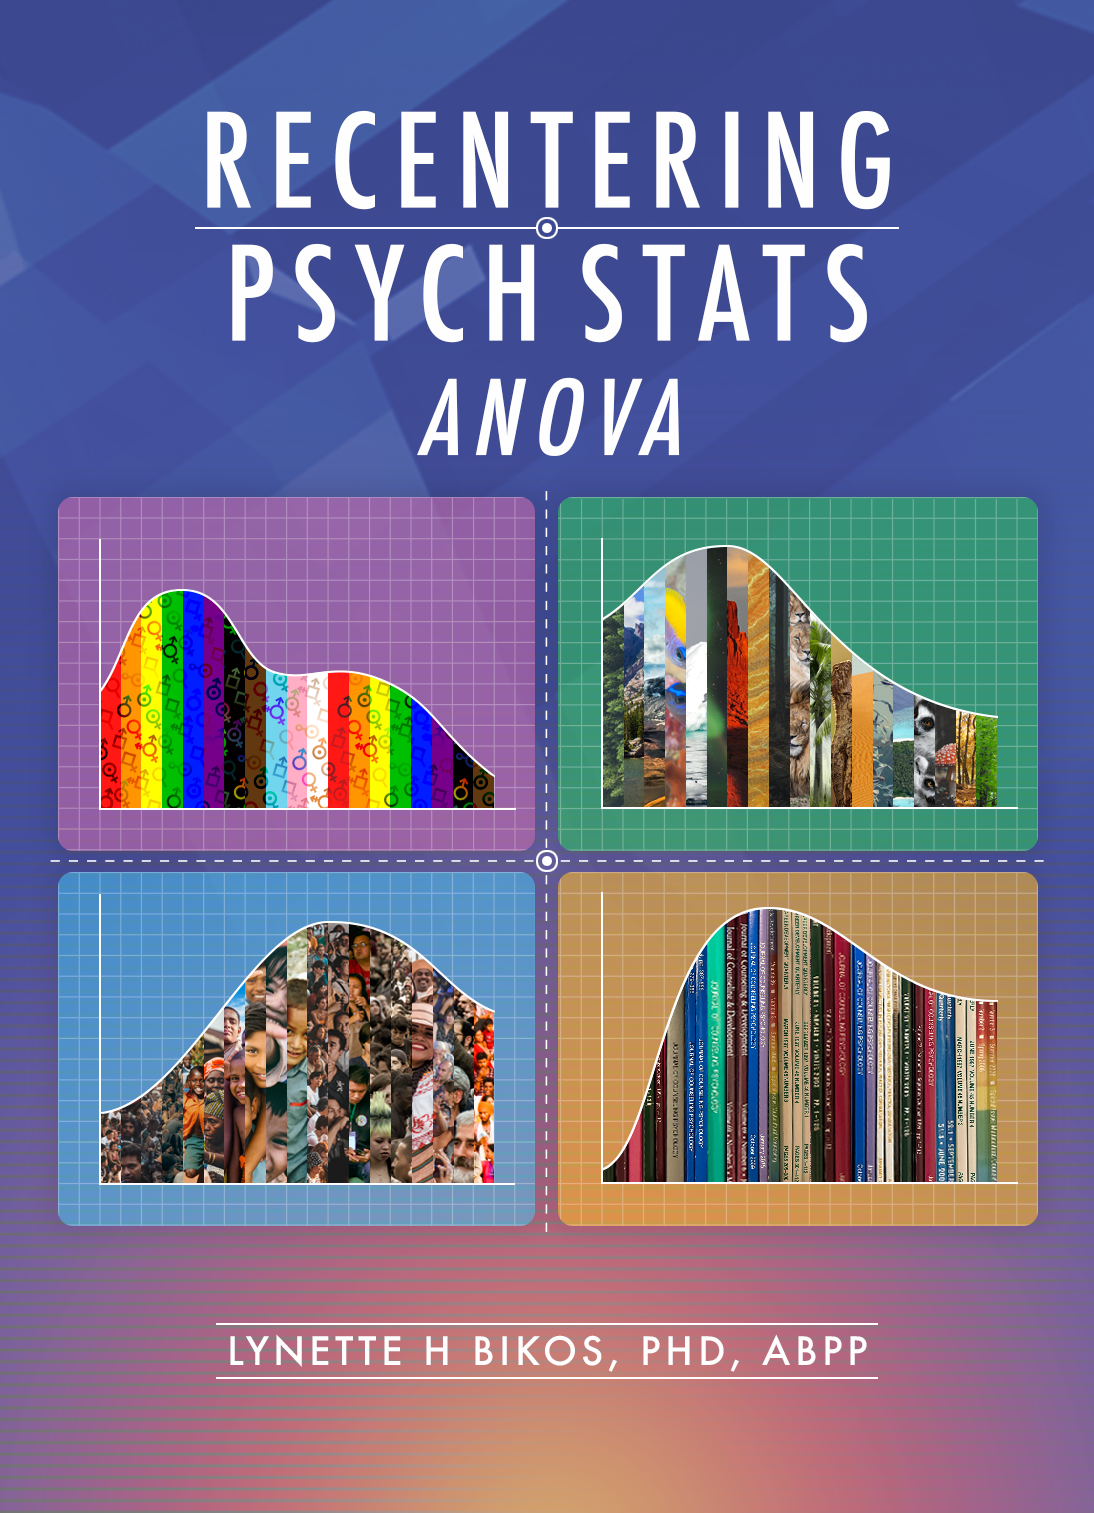
\includegraphics{images/ReC_ANOVA_bookcover.png}
This open education resource is available in three formats:

\begin{itemize}
\tightlist
\item
  Formatted as an \href{https://lhbikos.github.io/ReCenterPsychStats/}{html book} via GitHub Pages
\item
  As a \href{https://github.com/lhbikos/ReCenterPsychStats/blob/main/docs/ReCenterPsychStats.pdf}{PDF} available in the \href{https://github.com/lhbikos/ReCenterPsychStats/tree/main/docs}{docs} folder at the GitHub repository
\item
  As an \href{https://github.com/lhbikos/ReCenterPsychStats/blob/main/docs/ReCenterPsychStats.epub}{ebook} available in the \href{https://github.com/lhbikos/ReCenterPsychStats/tree/main/docs}{docs} folder at the GitHub repository
\end{itemize}

All materials used in creating this OER are available at its \href{https://github.com/lhbikos/ReCenterPsychStats}{GitHub repo}.

As a perpetually-in-progress, open education resource, feedback is always welcome. This IRB-approved (SPU IRB \#202102010R, no expiration) \href{https://spupsych.az1.qualtrics.com/jfe/form/SV_0OnBLfut3VIOIS2}{Qualtrics-hosted survey} includes formal rating scales, open-ended text boxes, and a portal for uploading attachments (e.g., marked up PDFs). You are welcome to complete only the portions that are relevant to you.

\hypertarget{preface}{%
\chapter*{PREFACE}\label{preface}}
\addcontentsline{toc}{chapter}{PREFACE}

\textbf{If you are viewing this document, you should know that this is a book-in-progress. Early drafts are released for the purpose teaching my classes and gaining formative feedback from a host of stakeholders. The document was last updated on 14 Jul 2022}. Emerging volumes on other statistics are posted on the \href{https://lhbikos.github.io/BikosRVT/ReCenter.html}{ReCentering Psych Stats} page at my research team's website.

\href{https://spu.hosted.panopto.com/Panopto/Pages/Viewer.aspx?id=c932455e-ef06-444a-bdca-acf7012d759a}{Screencasted Lecture Link}

To \emph{center} a variable in regression means to set its value at zero and interpret all other values in relation to this reference point. Regarding race and gender, researchers often center male and White at zero. Further, it is typical that research vignettes in statistics textbooks are similarly seated in a White, Western (frequently U.S.), heteronormative, framework. The purpose of this project is to create a set of open educational resources (OER) appropriate for doctoral and post-doctoral training that contribute to a socially responsive pedagogy -- that is, it contributes to justice, equity, diversity, and inclusion.

Statistics training in doctoral programs are frequently taught with fee-for-use programs (e.g., SPSS/AMOS, SAS, MPlus) that may not be readily available to the post-doctoral professional. In recent years, there has been an increase and improvement in R packages (e.g., \emph{psych}, \emph{lavaan}) used for analyses common to psychological research. Correspondingly, many graduate programs are transitioning to statistics training in R (free and open source). This is a challenge for post-doctoral psychologists who were trained with other software. This OER will offer statistics training with R and be freely available (specifically in a GitHub repository and posted through GitHub Pages) under a Creative Commons Attribution - Non Commercial - Share Alike license {[}CC BY-NC-SA 4.0{]}.

Training models for doctoral programs in health service psychology are commonly scholar-practitioner, scientist-practitioner, or clinical-scientist. An emerging model, the \emph{scientist-practitioner-advocacy} training model, incorporates social justice advocacy so that graduates are equipped to recognize and address the sociocultural context of oppression and unjust distribution of resources and opportunities \citep{mallinckrodt_scientist-practitioner-advocate_2014}. In statistics textbooks, the use of research vignettes engages the learner around a tangible scenario for identifying independent variables, dependent variables, covariates, and potential mechanisms of change. Many students recall examples in Field's \citeyearpar{field_discovering_2012} popular statistics text: Viagra to teach one-way ANOVA, beer goggles for two-way ANOVA, and bushtucker for repeated measures. What if the research vignettes were more socially responsive?

In this OER, research vignettes will be from recently published articles where:

\begin{itemize}
\tightlist
\item
  the author's identity is from a group where scholarship is historically marginalized (e.g., BIPOC, LGBTQ+, LMIC{[}low-middle income countries{]}),
\item
  the research is responsive to issues of justice, equity, inclusion, diversity,
\item
  the lesson's statistic is used in the article, and
\item
  there is sufficient information in the article to simulate the data for the chapter example(s) and practice problem(s); or it is publicly available.
\end{itemize}

In training for multicultural competence, the saying, ``A fish doesn't know that it's wet'' is often used to convey the notion that we are often unaware of our own cultural characteristics. In recent months and years, there has been an increased awakening to institutional and systemic factors that contribute to discrimination as a function of race, gender, nationality, class, and so forth. Queuing from the water metaphor, I am hopeful that a text that is recentered in the ways I have described can contribute to \emph{changing the water} in higher education and in the profession of psychology.

\hypertarget{copyright-with-open-access}{%
\section*{Copyright with Open Access}\label{copyright-with-open-access}}
\addcontentsline{toc}{section}{Copyright with Open Access}

This book is published under a a Creative Commons Attribution-NonCommercial-ShareAlike 4.0 International License. This means that this book can be reused, remixed, retained, revised and redistributed (including commercially) as long as appropriate credit is given to the authors. If you remix, or modify the original version of this open textbook, you must redistribute all versions of this open textbook under the same license: CC BY-SA 4.0.

A \href{https://github.com/lhbikos/ReCenterPsychStats}{GitHub open-source repository} contains all of the text and source code for the book, including data and images.

\hypertarget{acknowledgements}{%
\chapter*{ACKNOWLEDGEMENTS}\label{acknowledgements}}
\addcontentsline{toc}{chapter}{ACKNOWLEDGEMENTS}

As a doctoral student at the University of Kansas (1992-1996), I learned that ``a foreign language'' was a graduation requirement. \emph{Please note that as one who studies the intersections of global, vocational, and sustainable psychology, I regret that I do not have language skills beyond English.} This could have been met with credit from high school, but my rural, mid-Missouri high school did not offer such classes. This requirement would have typically been met with courses taken during an undergraduate program -- but my non-teaching degree in the University of Missouri's School of Education was exempt from this. The requirement could have also been met with a computer language (FORTRAN, C++) -- but I did not have any of those either. There was a tiny footnote on my doctoral degree plan that indicated that a 2-credit course, ``SPSS for Windows'' would substitute for the language requirement. Given that it was taught by my one of my favorite professors, I readily signed up. As it turns out, Samuel B. Green, PhD, was using the course to draft chapters in the textbook \citep{green_using_2014} that has been so helpful for so many. Unfortunately, Drs. Green (1947 - 2018) and Salkind (1947 - 2017) are no longer with us. I have worn out numerous versions of their text. Another favorite text of mine has been Dr.~Barbara Byrne's \citeyearpar{byrne_structural_2016}, ``Structural Equation Modeling with AMOS.'' I loved the way she worked through each problem and paired it with a published journal article, so that the user could see how the statistical evaluation fit within the larger project/article. I took my tea-stained text with me to a workshop she taught at APA and was proud of the signature she added to it. Dr.~Byrne created SEM texts for a number of statistical programs (e.g., LISREL, EQS, MPlus). As I was learning R, I wrote Dr.~Byrne, asking if she had an edition teaching SEM/CFA with R. She promptly wrote back, saying that she did not have the bandwidth to learn a new statistics package. We lost Dr.~Byrne in December 2020. I am so grateful to these role models for their contributions to my statistical training. I am also grateful for the doctoral students who have taken my courses and are continuing to provide input for how to improve the materials.

The inspiration for training materials that re*center statistics and research methods came from the \href{https://www.academics4blacklives.com/}{Academics for Black Survival and Wellness Initiative}. This project, co-founded by Della V. Mosley, Ph.D., and Pearis L. Bellamy, M.S., made clear the necessity and urgency for change in higher education and the profession of psychology.

At very practical levels, I am indebted to SPU's Library, and more specifically, SPU's Education, Technology, and Media Department. Assistant Dean for Instructional Design and Emerging Technologies, R. John Robertson, MSc, MCS, has offered unlimited consultation, support, and connection. Senior Instructional Designer in Graphics \& Illustrations, Dominic Wilkinson, designed the logo and bookcover. Psychology and Scholarly Communications Librarian, Kristin Hoffman, MLIS, has provided consultation on topics ranging from OERS to citations. I am alo indebted to Associate Vice President, Teaching and Learning at Kwantlen Polytechnic University, Rajiv Jhangiani, PhD. Dr.~Jhangiani's text \citeyearpar{jhangiani_research_2019} was the first OER I ever used and I was grateful for his encouraging conversation.

Financial support for this project has been provided the following:

\begin{itemize}
\tightlist
\item
  \emph{Call to Action on Equity, Inclusion, Diversity, Justice, and Social Responsivity Request for Proposals} grant from the Association of Psychology Postdoctoral and Internship Centers (2021-2022).
\item
  \emph{Diversity Seed Grant}, Office of Inclusive Excellence and Advisory Council for Diversity and Reconciliation (ACDR), Seattle Pacific University.
\item
  \emph{ETM Open Textbook \& OER Development Funding}, Office of Education, Technology, \& Media, Seattle Pacific University.
\end{itemize}

\hypertarget{ReCintro}{%
\chapter{Introduction}\label{ReCintro}}

\href{https://spu.hosted.panopto.com/Panopto/Pages/Viewer.aspx?pid=cc9b7c0d-e5c3-4e4e-a469-acf7013ee761}{Screencasted Lecture Link}

\hypertarget{what-to-expect-in-each-chapter}{%
\section{What to expect in each chapter}\label{what-to-expect-in-each-chapter}}

This textbook is intended as \emph{applied,} in that a primary goal is to help the scientist-practitioner-advocate use a variety of statistics in research problems and \emph{writing them up} for a program evaluation, dissertation, or journal article. In support of that goal, I try to provide just enough conceptual information so that the researcher can select the appropriate statistic (i.e., distinguishing between when ANOVA is appropriate and when regression is appropriate) and assign variables to their proper role (e.g., covariate, moderator, mediator).

This conceptual approach does include occasional, step-by-step, \emph{hand-calculations} (using R to do the math for us) to provide a \emph{visceral feeling} of what is happening within the statistical algorithm that may be invisible to the researcher. Additionally, the conceptual review includes a review of the assumptions about the characteristics of the data and research design that are required for the statistic.

Statistics can be daunting, so I have worked hard to establish a \emph{workflow} through each analysis. When possible, I include a flowchart that is referenced frequently in each chapter and assists the researcher keep track of their place in the many steps and choices that accompany even the simplest of analyses.

As with many statistics texts, each chapter includes a \emph{research vignette.} Somewhat unique to this resource is that the vignettes are selected from recently published articles. Each vignette is chosen with the intent to meet as many of the following criteria as possible:

\begin{itemize}
\tightlist
\item
  the statistic that is the focus of the chapter was properly used in the article,
\item
  the author's identity is from a group where scholarship is historically marginalized (e.g., BIPOC, LGBTQ+, LMIC {[}low middle income countries{]}),
\item
  the research has a justice, equity, inclusion, diversity, and social responsivity focus and will contribute positively to a social justice pedagogy, and
\item
  there is sufficient information in the article to simulate the data for the chapter example(s) and practice problem(s); or the data is available in a repository.
\end{itemize}

In each chapter we employ \emph{R} packages that will efficiently calculate the statistic and the dashboard of metrics (e.g., effect sizes, confidence intervals) that are typically reported in psychological science.

\hypertarget{strategies-for-accessing-and-using-this-oer}{%
\section{Strategies for Accessing and Using this OER}\label{strategies-for-accessing-and-using-this-oer}}

There are a number of ways you can access this resource. You may wish to try several strategies and then select which works best for you. I demonstrate these in the screencast that accompanies this chapter.

\begin{enumerate}
\def\labelenumi{\arabic{enumi}.}
\item
  Simply follow along in your preferred format of the book (html, PDF, or ebook) and then

  \begin{itemize}
  \tightlist
  \item
    open a fresh .rmd file of your own, copying (or retyping) the script and running it
  \end{itemize}
\item
  Locate the original documents at the \href{https://github.com/lhbikos/ReCenterPsychStats}{GitHub repository}. You can

  \begin{itemize}
  \tightlist
  \item
    open them to simply take note of the ``behind the scenes'' script
  \item
    copy/download individual documents that are of interest to you
  \item
    clone a copy of the entire project to your own GitHub site and further download it (in its entirety) to your personal workspace. The \href{https://desktop.github.com/}{GitHub Desktop app} makes this easy!
  \end{itemize}
\item
  Listen to the accompanying lectures (I think sound best when the speed is 1.75). The lectures are being recorded in Panopto and should include the closed captioning.
\item
  Each time the book is updated, new ebook and PDF versions are also pushed out. You can access these in the ``docs'' folder at the \href{https://github.com/lhbikos/ReCenterPsychStats}{GitHub repository}.
\item
  Provide feedback to me! If you fork a copy to your own GitHub repository, you can

  \begin{itemize}
  \tightlist
  \item
    open up an editing tool and mark up the document with your edits,
  \item
    start a discussion by leaving comments/questions, and then
  \item
    sending them back to me by committing and saving. I get an e-mail notiying me of this action. I can then review (accepting or rejecting) them and, if a discussion is appropriate, reply back to you.
  \item
    I am also seeking peer-review feedback at this \href{https://spupsych.az1.qualtrics.com/jfe/form/SV_0OnBLfut3VIOIS2}{Qualtrics-hosted survey}. You are welcome to complete only the portions that are relevant to you.
  \end{itemize}
\end{enumerate}

\hypertarget{if-you-are-new-to-r}{%
\section{If You are New to R}\label{if-you-are-new-to-r}}

R can be oveRwhelming. Jumping right into advanced statistics might not be the easiest way to start. The \href{https://lhbikos.github.io/ReCenterPsychStats/Ready.html}{Ready\_Set\_R}lesson of this volume provides an introduction and the \href{https://lhbikos.github.io/ReCenterPsychStats/waRmups.html}{waRming up}lesson walks through simple data preparation and descriptive statistics.

In the remaining lessons, I have attempted to provide complete code for every step of the process, starting with uploading the data. To help explain what R script is doing, I sometimes write it in the chapter text; sometimes leave hashtagged-comments in the chunks; and, particularly in the accompanying screencasted lectures, try to take time to narrate what the R script is doing.

I've found that, somewhere on the internet, there's almost always a solution to what I'm trying to do. I am frequently stuck and stumped and have spent hours searching the internet for even the tiniest of tasks. When you watch my videos, you may notice that in my R studio, there is a ``scRiptuRe'' file. I take notes on the solutions and scripts here -- using keywords that are meaningful to me so that when I need to repeat the task, I can hopefully search my own prior solutions and find a fix or a hint. You may also find it useful to create a working document of your own tips and tricks.

\hypertarget{Ready}{%
\chapter{Ready\_Set\_R}\label{Ready}}

\href{https://spu.hosted.panopto.com/Panopto/Pages/Viewer.aspx?pid=6b27a60c-edcb-4565-aaf1-ad890174586e}{Screencasted Lecture Link}

With the goal of creating a common, system-wide approach to using the platform, this lesson was originally created for Clinical and Industrial-Organizational doctoral students who are entering the ``stats sequence.'' I hope it will be useful for others (e.g., faculty, post-doctoral researchers, and practitioners) who are also making the transition to R.

\hypertarget{navigating-this-lesson}{%
\section{Navigating this Lesson}\label{navigating-this-lesson}}

There is about 45 minutes of lecture.

While the majority of R objects and data you will need are created within the R script that sources the chapter, occasionally there are some that cannot be created from within the R framework. Additionally, sometimes links fail. All original materials are provided at the \href{https://github.com/lhbikos/ReCenterPsychStats}{Github site} that hosts the book. More detailed guidelines for ways to access all these materials are provided in the OER's \protect\hyperlink{ReCintro}{introduction}

\hypertarget{learning-objectives}{%
\subsection{Learning Objectives}\label{learning-objectives}}

Learning objectives from this lecture include the following:

\begin{itemize}
\tightlist
\item
  Downloading/installing R's parts and pieces.
\item
  Using R-Markdown as the interface for running R analyses and saving the script.
\item
  Recognizing and adopting best practices for ``R hygiene.''
\item
  Identifying effective strategies for troubleshooting R hiccups.
\end{itemize}

\hypertarget{downloading-and-installing-r}{%
\section{downloading and installing R}\label{downloading-and-installing-r}}

\hypertarget{so-many-parts-and-pieces}{%
\subsection{So many paRts and pieces}\label{so-many-parts-and-pieces}}

Before we download R, it may be helpful to review some of R's many parts and pieces.

The base software is free and is available \href{https://www.r-project.org/}{here}

Because R is already on my machine (and because the instructions are sufficient), I will not walk through the demo, but I will point out a few things.

\begin{itemize}
\tightlist
\item
  The ``cran'' (I think ``cranium'') is the \emph{Comprehensive R Archive Network.} In order for R to run on your computer, you have to choose a location -- and it should be geographically ``close to you.''

  \begin{itemize}
  \tightlist
  \item
    Follow the instructions for your operating system (Mac, Windows, Linux)
  \item
    You will see the results of this download on your desktop (or elsewhere if you chose to not have it appear there) but you won't ever use R through this platform.
  \end{itemize}
\item
  \href{https://www.rstudio.com/products/RStudio/}{R Studio} is the way in which we operate R. It's a separate download. Choose the free, desktop, option that is appropriate for your operating system:\\
\item
  \emph{R Markdown} is the way that many analysts write \emph{script}, conduct analyses, and even write up results. These are saved as .rmd files.

  \begin{itemize}
  \tightlist
  \item
    In R Studio, open an R Markdown document through File/New File/R Markdown
  \item
    Specify the details of your document (title, author, desired ouput)
  \item
    In a separate step, SAVE this document (File/Save{]} into a NEW FILE FOLDER that will contain anything else you need for your project (e.g., the data).
  \item
    \emph{Packages} are at the heart of working in R. Installing and activating packages require writing script.
  \end{itemize}
\end{itemize}

\textbf{Note} If you have an enterprise-owned machine (e.g,. in my specific context, if you are a faculty/staff or have a lab with institution-issued laptops) there can be complications caused by how documents are stored. In recent years we have found that letting the computer choose where to load base R, R Studio, and the packages generally works. The trick, though, is to save R projects (i.e., folder with .rmd files and data) into the OneDrive folder that syncs to your computer. If you have difficulty knitting that is unrelated to code (verified by getting a classmates or colleague to successfully knit it), it is likely because you have saved the files to the local hard drive and not OneDrive. If you continue to have problems I recommend consulting with your computer and technology support office.

\hypertarget{orienting-to-r-studio-focusing-only-on-the-things-we-will-be-using-first-and-most-often}{%
\subsection{oRienting to R Studio (focusing only on the things we will be using first and most often)}\label{orienting-to-r-studio-focusing-only-on-the-things-we-will-be-using-first-and-most-often}}

R Studio is organized around four panes. These can be sized and rearranged to suit your personal preferences.

\begin{itemize}
\tightlist
\item
  Upper right window

  \begin{itemize}
  \tightlist
  \item
    Environment: lists the \emph{objects} that are available to you (e.g., dataframes)
  \end{itemize}
\item
  Lower right window
\item
  \emph{Files}: Displays the file structure in your computer's environment. Make it a practice to (a) organize your work in small folders and (b) navigating to that small folder that is holding your project when you are working on it.
\item
  \emph{Packages}: Lists the packages that have been installed. If you navigate to it, you can see if it is ``on.'' You can also access information about the package (e.g., available functions, examples of script used with the package) in this menu. This information opens in the Help window.
\item
  The \emph{Viewer} and \emph{Plots} tabs will be useful, later, in some advanced statistics when we can simultaneously examine output and script in windows that are side-by-side.
\item
  Upper left window

  \begin{itemize}
  \tightlist
  \item
    If you are using R Markdown, that file lives here and is composed of open space and chunks.
  \end{itemize}
\item
  Lower left window

  \begin{itemize}
  \tightlist
  \item
    R Studio runs in the Console (the background). Very occasionally, I can find useful troubleshooting information here.
  \item
    More commonly, I open my R Markdown document so that it takes the whole screen.
  \end{itemize}
\end{itemize}

\hypertarget{best-practices}{%
\section{best pRactices}\label{best-practices}}

Many initial problems in R can be solved with good R hygiene. Here are some suggestions for basic practices. It can be tempting to ``skip this.'' However, in the first few weeks of class, these are the solutions I am presenting (and repeating, ad nauseum) to my students.

\hypertarget{everything-is-documented-in-the-.rmd-file}{%
\subsection{Everything is documented in the .rmd file}\label{everything-is-documented-in-the-.rmd-file}}

Although others do it differently, I put everything is in my .rmd file. That is, for uploading data I write the code in my .rmd file. For opening packages, I include the package in my script. I also use the .rmd file to make notes about what I was thinking and why I made the choices I did. I also keep a ``bug log'' -- noting what worked and what did not work. I will also begin my APA style results section directly in the .rmd file.

Why do I do all this? Because when I return to my project hours or years later, I have a permanent record of very critical things like (a) where my data is located, (b) what version I was using, and (c) what package was associated with the functions.

\hypertarget{setting-up-the-file}{%
\subsection{Setting up the file}\label{setting-up-the-file}}

File organization is a critical key to success:

\begin{itemize}
\tightlist
\item
  Create a project file folder.
\item
  Put the data file in it.
\item
  Open an R Markdown file.
\item
  Save it in the same file folder.
\item
  When your data and .rmd files are in the same folder (not your desktop, but a shared folder) the data can be pulled into the .rmd file without creating a working directory.
\end{itemize}

\hypertarget{script-in-chunks-and-everything-else-in-the-inline-text-sections}{%
\subsection{Script in chunks and everything else in the ``inline text'' sections}\label{script-in-chunks-and-everything-else-in-the-inline-text-sections}}

The R Markdown document is an incredible tool for integrating text, tables, and analyses. This entire OER is written in R Markdown. A central feature of this is ``chunks.''

The only thing in the chunks should be script for running R. You can also hashtag-out comments so they won't run.

You can put almost anything you want in the ``inline text with simple formatting.'' Syntax for simple formatting in the text areas (e.g., using italics, making headings, bold) is found here: \url{https://rmarkdown.rstudio.com/authoring_basics.html}

``Chunks'' start and end with with three tic marks and will show up in a shaded box. Chunks have three symbols in their upper right. Those controls will disappear and your script will not run) if you have replaced them with double or single quotation marks or one or more of the tics are missing.

The easiest way to insert a chunk is to use the INSERT/R command at the top of this editor box. You can also insert a chunk with the keyboard shortcut: CTRL/ALT/i

\begin{Shaded}
\begin{Highlighting}[]
\CommentTok{\#hashtags let me write comments to remind myself what I did}
\CommentTok{\#here I am simply demonstrating arithmetic (but I would normally be running code)}
\DecValTok{2021} \SpecialCharTok{{-}} \DecValTok{1966}
\end{Highlighting}
\end{Shaded}

\begin{verbatim}
[1] 55
\end{verbatim}

\hypertarget{managing-packages}{%
\subsection{Managing packages}\label{managing-packages}}

As scientist-practitioners (and not coders), we will rely on \emph{packages} to do much of the work. At first you may feel overwhelmed about the large number of packages that are available. Soon, though, you will become accustomed to the ones most applicable to our work (e.g., psych, tidyverse, lavaan, apaTables).

Researchers treat packages differently. In these lectures, I list all the packages we will use in an opening chunk at the beginning of the lecture. When the hashtags are removed, the script will ask R to check to see if the package is installed. If it is, installation is skipped. If it is not, R installs it. Simply remove the hashtag to run the code the first time, then hashtag them back out so R is not always re-checking.

\begin{Shaded}
\begin{Highlighting}[]
\CommentTok{\# will install the package if not already installed}
\CommentTok{\# if(!require(psych))\{install.packages(\textquotesingle{}psych\textquotesingle{})\}}
\end{Highlighting}
\end{Shaded}

To make a package operable, you need to open it. There are two primary ways to do this. The first is to use the library function.

\begin{Shaded}
\begin{Highlighting}[]
\CommentTok{\#install.packages ("psych")}
\FunctionTok{library}\NormalTok{ (psych)}
\end{Highlighting}
\end{Shaded}

The second way is to place a double colon between the package and function. This second method has become my preferred practice because it helps me remember what package goes with each function. It can also prevent R hiccups when there are identical function names and R does not know which package to use. Below is an example where I might ask for descriptives from the psych package. Because I have not yet uploaded data, I have hashtagged it out, making the command inoperable.

\begin{Shaded}
\begin{Highlighting}[]
\CommentTok{\#psych::describe(mydata)}
\end{Highlighting}
\end{Shaded}

There are exceptions. One is the \emph{tidyverse} package. Some of my script uses pipes (\%\textgreater\%) and they require tidyverse to be activated this is why you will often see me call the tidyverse package with the \emph{library()} function (as demonstrated above.)

\hypertarget{upload-the-data}{%
\subsection{Upload the data}\label{upload-the-data}}

When imported (or simulated) properly, data will appear as an object in the global environment.

In the context of this OER, I will be simulating data right in each lesson for use in the lesson. This makes the web-based platform more \emph{portable.} This means that when working the problems in the chapter we do not (a) write the data to a file and (b) import data from files. Because these are essential skills, I will demonstrate this process here -- starting with simulating data.

At this point, simulating data is beyond the learning goals I have established for the chapter. I do need to include the code so that we get some data. The data I am simulating is used in the \protect\hyperlink{oneway}{one-way ANOVA lesson}. The data is from the Tran and Lee \citeyearpar{tran_you_2014} random clinical trial.

In this simulation, I am simply creating an ID number, a condition (High, Low, Control), and a score on the dependent variable, ``Accurate.'' More information about this study is included in the \protect\hyperlink{oneway}{one-way ANOVA chapter}.

\begin{Shaded}
\begin{Highlighting}[]
\CommentTok{\# Note, this simulation results in a different datset than is in the}
\CommentTok{\# OnewayANOVA lesson sets a random seed so that we get the same}
\CommentTok{\# results each time}
\FunctionTok{set.seed}\NormalTok{(}\DecValTok{2021}\NormalTok{)}
\CommentTok{\# sample size, M and SD for each group}
\NormalTok{Accurate }\OtherTok{\textless{}{-}} \FunctionTok{c}\NormalTok{(}\FunctionTok{rnorm}\NormalTok{(}\DecValTok{30}\NormalTok{, }\AttributeTok{mean =} \FloatTok{1.18}\NormalTok{, }\AttributeTok{sd =} \FloatTok{0.8}\NormalTok{), }\FunctionTok{rnorm}\NormalTok{(}\DecValTok{30}\NormalTok{, }\AttributeTok{mean =} \FloatTok{1.83}\NormalTok{,}
    \AttributeTok{sd =} \FloatTok{0.58}\NormalTok{), }\FunctionTok{rnorm}\NormalTok{(}\DecValTok{30}\NormalTok{, }\AttributeTok{mean =} \FloatTok{1.76}\NormalTok{, }\AttributeTok{sd =} \FloatTok{0.56}\NormalTok{))}
\CommentTok{\# set upper bound for DV}
\NormalTok{Accurate[Accurate }\SpecialCharTok{\textgreater{}} \DecValTok{3}\NormalTok{] }\OtherTok{\textless{}{-}} \DecValTok{3}
\CommentTok{\# set lower bound for DV}
\NormalTok{Accurate[Accurate }\SpecialCharTok{\textless{}} \DecValTok{0}\NormalTok{] }\OtherTok{\textless{}{-}} \DecValTok{0}
\CommentTok{\# IDs for participants}
\NormalTok{ID }\OtherTok{\textless{}{-}} \FunctionTok{factor}\NormalTok{(}\FunctionTok{seq}\NormalTok{(}\DecValTok{1}\NormalTok{, }\DecValTok{90}\NormalTok{))}
\CommentTok{\# name factors and identify how many in each group; should be in same}
\CommentTok{\# order as first row of script}
\NormalTok{COND }\OtherTok{\textless{}{-}} \FunctionTok{c}\NormalTok{(}\FunctionTok{rep}\NormalTok{(}\StringTok{"High"}\NormalTok{, }\DecValTok{30}\NormalTok{), }\FunctionTok{rep}\NormalTok{(}\StringTok{"Low"}\NormalTok{, }\DecValTok{30}\NormalTok{), }\FunctionTok{rep}\NormalTok{(}\StringTok{"Control"}\NormalTok{, }\DecValTok{30}\NormalTok{))}
\CommentTok{\# groups the 3 variables into a single df: ID, DV, condition}
\NormalTok{Acc\_sim30 }\OtherTok{\textless{}{-}} \FunctionTok{data.frame}\NormalTok{(ID, COND, Accurate)}
\end{Highlighting}
\end{Shaded}

At this point, this data lives only in this .rmd file after the above code is run. Although there are numerous ways to export and import data, I have a preference for two.

\hypertarget{to-and-from-.csv-files}{%
\subsubsection{To and from .csv files}\label{to-and-from-.csv-files}}

The first is to write the data to a .csv file. In your computer's environment (outside of R), these files are easily manipulated in Excel. I think of them as being ``Excel lite'' because although Excel can operate them, they lack some of the more advanced features of an Excel spreadsheet.

In the code below, I identify the R object ``Acc\_sim30'' and give it a file name, ``to\_CSV.csv''. This file name must have the .csv extension. I also indicate that it should preserve the column names (but ignore row names; since we don't have row names).

This file will save in the same folder as wherever you are using this .rmd file.

\begin{Shaded}
\begin{Highlighting}[]
\CommentTok{\# to write it to an outfile as a .csv}
\FunctionTok{write.table}\NormalTok{(Acc\_sim30, }\AttributeTok{file =} \StringTok{"to\_CSV.csv"}\NormalTok{, }\AttributeTok{sep =} \StringTok{","}\NormalTok{, }\AttributeTok{col.names =} \ConstantTok{TRUE}\NormalTok{,}
    \AttributeTok{row.names =} \ConstantTok{FALSE}\NormalTok{)}
\end{Highlighting}
\end{Shaded}

Importing this object back into the R environment can be accomplished with some simple code. For the sake of demonstration,

\begin{Shaded}
\begin{Highlighting}[]
\CommentTok{\# to save the df as an .csv (think \textquotesingle{}Excel lite\textquotesingle{}) file on your}
\CommentTok{\# computer; it should save in the same file as the .rmd file you are}
\CommentTok{\# working with}
\NormalTok{from\_CSV }\OtherTok{\textless{}{-}} \FunctionTok{read.csv}\NormalTok{(}\StringTok{"to\_CSV.csv"}\NormalTok{, }\AttributeTok{header =} \ConstantTok{TRUE}\NormalTok{)}
\end{Highlighting}
\end{Shaded}

The advantage of working with .csv files is that it is then easy to inspect and manipulate them outside of the R environment. The disadvantage of .csv files is that each time they are imported they lose any formatting you may have meticulously assigned to them.

\hypertarget{to-and-from-.rds-files}{%
\subsubsection{To and from .rds files}\label{to-and-from-.rds-files}}

While it is easy enough to rerun the code (or copy it from data prep .rmd and paste it into an .rmd you are using for advanced analysis), there is a better way! Saving the data as an R object preserves all of its characteristics.

\begin{Shaded}
\begin{Highlighting}[]
\CommentTok{\# to save the df as an .rds file on your computer; it should save in}
\CommentTok{\# the same file as the .rmd file you are working with}
\FunctionTok{saveRDS}\NormalTok{(Acc\_sim30, }\StringTok{"to\_Robject.rds"}\NormalTok{)}
\end{Highlighting}
\end{Shaded}

This file will save to your computer (and you can send it to colleagues). However, it is not easy to ``just open it'' in Excel. To open an .rds file and use it (whether you created it or it is sent to you by a colleague), use the following code:

\begin{Shaded}
\begin{Highlighting}[]
\NormalTok{from\_rds }\OtherTok{\textless{}{-}} \FunctionTok{readRDS}\NormalTok{(}\StringTok{"to\_Robject.rds"}\NormalTok{)}
\end{Highlighting}
\end{Shaded}

If you are the recipient of an R object, but want to view it as a .csv, simply import the .rds then use the above code to export it as a .csv.

\hypertarget{from-spss-files}{%
\subsubsection{From SPSS files}\label{from-spss-files}}

Your data may come to you in a variety of ways. One of the most common is SPSS. The \emph{foreign} package is popular for importing SPSS data. Below is code which would import an SPSS file \emph{if I had created one}. You'll see that this script is hashtagged out because I rarely use SPSS and do not have a handy file to demo.

\begin{Shaded}
\begin{Highlighting}[]
\CommentTok{\# opening an SPSS file requires the foreign package which I opened}
\CommentTok{\# earlier from\_SPSS \textless{}{-} foreign::read.spss (\textquotesingle{}SPSSdata.sav\textquotesingle{},}
\CommentTok{\# use.value.labels = TRUE, to.data.frame = TRUE)}
\end{Highlighting}
\end{Shaded}

\hypertarget{quick-demonstration}{%
\section{quick demonstRation}\label{quick-demonstration}}

Let's run some simple descriptives. In the script below, I am using the \emph{psych} package. Descriptive statistics will appear for all the data in the dataframe and the output will be rounded to three spaces. Note that rather than opening the psych package with the library function, I have used the double colon convention.

\begin{Shaded}
\begin{Highlighting}[]
\FunctionTok{round}\NormalTok{(psych}\SpecialCharTok{::}\FunctionTok{describe}\NormalTok{(Acc\_sim30), }\DecValTok{3}\NormalTok{)}
\end{Highlighting}
\end{Shaded}

\begin{verbatim}
         vars  n  mean    sd median trimmed   mad min max range  skew kurtosis
ID*         1 90 45.50 26.12  45.50   45.50 33.36   1  90    89  0.00    -1.24
COND*       2 90  2.00  0.82   2.00    2.00  1.48   1   3     2  0.00    -1.53
Accurate    3 90  1.52  0.68   1.55    1.54  0.70   0   3     3 -0.19    -0.34
           se
ID*      2.75
COND*    0.09
Accurate 0.07
\end{verbatim}

Because ``ID'' is the case ID and COND is the factor (high, low, control), the only variable for which this data is sensible is ``Accurate.'' Nonetheless, this provides an example of how to apply a package's function to a dataset. As we progress through the text we will learn how to manage the data so that we get the specific output we are seeking.

\hypertarget{the-knitted-file}{%
\section{the knitted file}\label{the-knitted-file}}

One of the coolest things about R Markdown is its capacity to \emph{knit} to HTML, PPT, or WORD.

\begin{itemize}
\tightlist
\item
  In this OER, I am writing the lessons in R markdown (.rmd files), with the package \emph{bookdown} as a helper, and knitting the files to the .html format. In prior years, I knitted these documents to .doc formats. There are numerous possibilities!
\item
  The package \emph{papaja} is designed to prepare APA manuscripts where the writing, statistics, and references are all accomplished in a single file. This process contributes to replicability and reproducibility.
\item
  If you are using the PDF or ebook version of this OER you will realize that it is also possible to render to these formats. Albeit slighy more complicated, this is possible, too! More detailed instructions for this are provided in the \href{https://lhbikos.github.io/extRas/}{extRas} mini-volume of \href{https://lhbikos.github.io/BikosRVT/ReCenter.html}{ReCentering Psych Stats}.
\end{itemize}

\hypertarget{troubleshooting-in-r-markdown}{%
\section{tRoubleshooting in R maRkdown}\label{troubleshooting-in-r-markdown}}

Hiccups are normal. Here are some ideas that I have found useful in getting unstuck.

\begin{itemize}
\tightlist
\item
  In a given set of operations, you must run/execute each piece of code in order: every, single, time. That is, all the packages have to be in your library and activated.

  \begin{itemize}
  \tightlist
  \item
    If you open an .rmd file, you cannot just scroll down to make a boxplot. You need to run any \emph{prerequisite} script (like loading files, putting the data in the global environment, etc.)
  \item
    Lost? Clear your global environment (broom icon in the upper right) and start over. Fresh starts are good.
  \end{itemize}
\item
  Your .rmd file and your data need to be stored in the same file folder. Make unique folders for each project (even if each contains only a few files).
\item
  If you have tried what seems apparent to you and cannot solve your challenge, do not wait long before typing warnings into a search engine. Odds are, you'll get some useful hints in a manner of seconds. Especially at first, these are common errors:

  \begin{itemize}
  \tightlist
  \item
    The package isn't loaded.
  \item
    The .rmd file hasn't been saved yet, or isn't saved in the same folder as the data.
  \item
    There are errors in punctuation or spelling.
  \end{itemize}
\item
  Restart R (it's quick -- not like restarting your computer). I like to restart and clear my output and environment so that I can better track my order of operations.
\item
  If you receive an error indicating that a function isn't working or recognized, and you have loaded the package, type the name of the package in front of the function with two colons (e.g., psych::describe(df)). If multiple packages are loaded with functions that have the same name, R can get confused.
\end{itemize}

\hypertarget{just-why-have-we-transitioned-to-r}{%
\section{\texorpdfstring{just \emph{why} have we tRansitioned to R?}{just why have we tRansitioned to R?}}\label{just-why-have-we-transitioned-to-r}}

\begin{itemize}
\tightlist
\item
  It (or at least it appears to be) is the futuRe.
\item
  SPSS site (and individual) licenses are increasingly expensive and limited (e.g., we need Mplus, AMOS, HLM, or R). As package development for R is exploding, we have tools to ``do just about anything.''
\item
  Most graduate psychology programs are scientist/practitioner in nature and include training in ``high end'' statistics. Yet, many of your employing organizations will not have SPSS. R is a free, universally accessible program, that our graduates can use anywhere.
\end{itemize}

\hypertarget{strategies-for-success}{%
\section{stRategies for success}\label{strategies-for-success}}

\begin{itemize}
\tightlist
\item
  Engage with R, but don't let it overwhelm you.

  \begin{itemize}
  \tightlist
  \item
    The \emph{mechanical is also the conceptual}. Especially while it's \emph{simpler}, do try to retype the script into your own .rmd file and run it. Track down the errors you are making and fix them.
  \item
    If this stresses you out, move to simply copying the code into the .rmd file and running it. If you continue to have errors, you may have violated one of the best practices above (ask, ``Is the package activated?'' ``Are the data and .rmd files in the same place?'' ``Is all the prerequisite script run?'').
  \item
    Still overwhelmed? Keep moving forward by (retrieving the original.rmd file from the GitHub repository) opening a copy of the .rmd file and just ``run it along'' with the lecture. Spend your mental power trying to understand what each piece does so you can translate it for any homework assignments. My suggestions for practice aspire to be parallel to the lecture with no sneaky trix.
  \end{itemize}
\item
  Copy script that works elsewhere and replace it with your datafile, variables, and so forth.
\item
  The leaRning curve is steep, but not impossible. Gladwell \citeyearpar{gladwell_outliers_2008} taught us that it takes about 10,000 hours to get great at something (2,000 to get reasonably competent). Practice. Practice. Practice.
\item
  Updates to R, R Studio, and the packages are necessary, but can also be problematic. Sometimes updates cause programs/script to fail (e.g., ``X has been deprecated for version X.XX''). My personal practice is to update R, R Studio, and the packages a week or two before each academic term. I expect that prior scripts may need to be updated or revised with package updates and incongruencies between base R, R Studio, and the packages.
\item
  Embrace your downward dog. And square breathing. Also, walk away, then come back.
\end{itemize}

\hypertarget{resources-for-getting-started}{%
\section{Resources for getting staRted}\label{resources-for-getting-started}}

R for Data Science: \url{https://r4ds.had.co.nz/}

R Cookbook: \url{http://shop.oreilly.com/product/9780596809164.do}

R Markdown homepage with tutorials: \url{https://rmarkdown.rstudio.com/index.html}

R has cheatsheets for everything, here's the one for R Markdown: \url{https://www.rstudio.com/wp-content/uploads/2015/02/rmarkdown-cheatsheet.pdf}

R Markdown Reference guide: \url{https://www.rstudio.com/wp-content/uploads/2015/03/rmarkdown-reference.pdf}

Using R Markdown for writing reproducible scientific papers: \url{https://libscie.github.io/rmarkdown-workshop/handout.html}

Script for all of Field's text: \url{https://studysites.uk.sagepub.com/dsur/study/scriptfi.htm}

LaTeX equation editor: \url{https://www.codecogs.com/latex/eqneditor.php}

\hypertarget{waRmups}{%
\chapter{waRming up}\label{waRmups}}

\href{https://spu.hosted.panopto.com/Panopto/Pages/Viewer.aspx?pid=45cedbad-3504-439b-a9b2-ad89017fcc5a}{Screencasted Lecture Link}

The beginning of any data analysis means familiarizing yourself with the data, that is, its distributional characteristics as well as its relations.

\hypertarget{navigating-this-lesson-1}{%
\section{Navigating this Lesson}\label{navigating-this-lesson-1}}

There is about 25 minutes of lecture.

While the majority of R objects and data you will need are created within the R script that sources the chapter, occasionally there are some that cannot be created from within the R framework. Additionally, sometimes links fail. All original materials are provided at the \href{https://github.com/lhbikos/ReCenterPsychStats}{Github site} that hosts the book. More detailed guidelines for ways to access all these materials are provided in the OER's \protect\hyperlink{ReCintro}{introduction}

\hypertarget{learning-objectives-1}{%
\subsection{Learning Objectives}\label{learning-objectives-1}}

Learning objectives from this lecture include the following:

\begin{itemize}
\tightlist
\item
  Produce descriptive statistics (means, standard deviations, skew, kurtosis), and correlation matrix, with the \emph{psych} package
\item
  Produce plots of data
\item
  Interpret skew, kurtosis, correlations
\item
  Create an APA Style table and results section that includes means, standard deviations, and correlations
\end{itemize}

\hypertarget{planning-for-practice}{%
\subsection{Planning for Practice}\label{planning-for-practice}}

This is designed as a ``get (or `get back') into it'' assignment. You will essentially work through this very same lecture, using the same dataframe -- just a different set of continuous variables.

\hypertarget{readings-resources}{%
\subsection{Readings \& Resources}\label{readings-resources}}

In preparing this chapter, I drew heavily from the following resource(s). Other resources are cited (when possible, linked) in the text with complete citations in the reference list.

\begin{itemize}
\tightlist
\item
  Revelle, W. (2021). An introduction to the psych package: Part I: data entry and data description. 60.

  \begin{itemize}
  \tightlist
  \item
    Revelle is the author/creator of the \emph{psych} package. His tutorial provides both technical and interpretive information. Read pages 1-17.
  \end{itemize}
\item
  Lui, P. P. (2020). Racial microaggression, overt discrimination, and distress: (In)Direct associations with psychological adjustment. \emph{The Counseling Psychologist, 32}.

  \begin{itemize}
  \tightlist
  \item
    This is the research vignette from which I simulate data that we can use in the lesson and practice problem.
  \end{itemize}
\end{itemize}

\hypertarget{research-vignette}{%
\section{Research Vignette}\label{research-vignette}}

We will use simulated data from Lui \citeyearpar{lui_racial_2020} for simple data screening. Controlling for overt discrimination, and neuroticism, Lui examined the degree to which racial microaggressions contributed to negative affect, alcohol consumption, and drinking problems in African American, Asian American, and Latinx American college students (\emph{N} = 713).

Using the means, standard deviations, correlation matrix, and group sizes (\emph{n}) I simulated the data. While the process of simulation is beyond the learning goals of this lesson (you can skip that part), I include it here so that it is easy to work the rest of the script.

\begin{Shaded}
\begin{Highlighting}[]
\FunctionTok{set.seed}\NormalTok{(}\DecValTok{210807}\NormalTok{)  }\CommentTok{\#sets the random seed so that we consistently get the same results}
\CommentTok{\# for practice, you could change (or remove) the random seed and try}
\CommentTok{\# to interpret the results (they should be quite similar) There are}
\CommentTok{\# probably more efficient ways to simulate data. Given the}
\CommentTok{\# information available in the manuscript, my approach was to first}
\CommentTok{\# create the datasets for each of the racial ethnic groups that were}
\CommentTok{\# provided and then binding them together.}

\CommentTok{\# First, the data for the students who identified as Asian American}
\NormalTok{Asian\_mu }\OtherTok{\textless{}{-}} \FunctionTok{c}\NormalTok{(}\FloatTok{1.52}\NormalTok{, }\FloatTok{1.72}\NormalTok{, }\FloatTok{2.69}\NormalTok{, }\FloatTok{1.71}\NormalTok{, }\FloatTok{2.14}\NormalTok{, }\FloatTok{2.35}\NormalTok{, }\FloatTok{2.42}\NormalTok{)}
\NormalTok{Asian\_stddev }\OtherTok{\textless{}{-}} \FunctionTok{c}\NormalTok{(}\FloatTok{2.52}\NormalTok{, }\FloatTok{2.04}\NormalTok{, }\FloatTok{0.47}\NormalTok{, }\FloatTok{0.7}\NormalTok{, }\FloatTok{0.8}\NormalTok{, }\FloatTok{2.41}\NormalTok{, }\FloatTok{3.36}\NormalTok{)}
\NormalTok{Asian\_corMat }\OtherTok{\textless{}{-}} \FunctionTok{matrix}\NormalTok{(}\FunctionTok{c}\NormalTok{(}\DecValTok{1}\NormalTok{, }\FloatTok{0.69}\NormalTok{, }\FloatTok{0.19}\NormalTok{, }\FloatTok{0.28}\NormalTok{, }\FloatTok{0.32}\NormalTok{, }\FloatTok{0.08}\NormalTok{, }\FloatTok{0.23}\NormalTok{, }\FloatTok{0.69}\NormalTok{, }\DecValTok{1}\NormalTok{,}
    \FloatTok{0.2}\NormalTok{, }\FloatTok{0.29}\NormalTok{, }\FloatTok{0.33}\NormalTok{, }\FloatTok{0.13}\NormalTok{, }\FloatTok{0.25}\NormalTok{, }\FloatTok{0.19}\NormalTok{, }\FloatTok{0.2}\NormalTok{, }\DecValTok{1}\NormalTok{, }\FloatTok{0.5}\NormalTok{, }\FloatTok{0.5}\NormalTok{, }\SpecialCharTok{{-}}\FloatTok{0.04}\NormalTok{, }\FloatTok{0.09}\NormalTok{, }\FloatTok{0.28}\NormalTok{,}
    \FloatTok{0.29}\NormalTok{, }\FloatTok{0.5}\NormalTok{, }\DecValTok{1}\NormalTok{, }\FloatTok{0.76}\NormalTok{, }\FloatTok{0.04}\NormalTok{, }\FloatTok{0.18}\NormalTok{, }\FloatTok{0.32}\NormalTok{, }\FloatTok{0.33}\NormalTok{, }\FloatTok{0.5}\NormalTok{, }\FloatTok{0.76}\NormalTok{, }\DecValTok{1}\NormalTok{, }\FloatTok{0.1}\NormalTok{, }\FloatTok{0.21}\NormalTok{,}
    \FloatTok{0.08}\NormalTok{, }\FloatTok{0.13}\NormalTok{, }\SpecialCharTok{{-}}\FloatTok{0.04}\NormalTok{, }\FloatTok{0.04}\NormalTok{, }\FloatTok{0.1}\NormalTok{, }\DecValTok{1}\NormalTok{, }\FloatTok{0.42}\NormalTok{, }\FloatTok{0.23}\NormalTok{, }\FloatTok{0.25}\NormalTok{, }\FloatTok{0.09}\NormalTok{, }\FloatTok{0.18}\NormalTok{, }\FloatTok{0.21}\NormalTok{,}
    \FloatTok{0.42}\NormalTok{, }\DecValTok{1}\NormalTok{), }\AttributeTok{ncol =} \DecValTok{7}\NormalTok{)}
\NormalTok{Asian\_covMat }\OtherTok{\textless{}{-}}\NormalTok{ Asian\_stddev }\SpecialCharTok{\%*\%} \FunctionTok{t}\NormalTok{(Asian\_stddev) }\SpecialCharTok{*}\NormalTok{ Asian\_corMat}

\NormalTok{Asian\_dat }\OtherTok{\textless{}{-}}\NormalTok{ MASS}\SpecialCharTok{::}\FunctionTok{mvrnorm}\NormalTok{(}\AttributeTok{n =} \DecValTok{398}\NormalTok{, }\AttributeTok{mu =}\NormalTok{ Asian\_mu, }\AttributeTok{Sigma =}\NormalTok{ Asian\_covMat,}
    \AttributeTok{empirical =} \ConstantTok{TRUE}\NormalTok{)}
\NormalTok{Asian\_df }\OtherTok{\textless{}{-}} \FunctionTok{as.data.frame}\NormalTok{(Asian\_dat)}

\FunctionTok{library}\NormalTok{(tidyverse)}
\NormalTok{Asian\_df }\OtherTok{\textless{}{-}} \FunctionTok{rename}\NormalTok{(Asian\_df, }\AttributeTok{OvDisc =}\NormalTok{ V1, }\AttributeTok{mAggr =}\NormalTok{ V2, }\AttributeTok{Neuro =}\NormalTok{ V3, }\AttributeTok{nAff =}\NormalTok{ V4,}
    \AttributeTok{psyDist =}\NormalTok{ V5, }\AttributeTok{Alcohol =}\NormalTok{ V6, }\AttributeTok{drProb =}\NormalTok{ V7)}
\NormalTok{Asian\_df}\SpecialCharTok{$}\NormalTok{RacEth }\OtherTok{\textless{}{-}} \StringTok{"Asian"}

\CommentTok{\# Second, the data for the students who identified as Black/African}
\CommentTok{\# American}
\NormalTok{Black\_mu }\OtherTok{\textless{}{-}} \FunctionTok{c}\NormalTok{(}\FloatTok{4.45}\NormalTok{, }\FloatTok{3.84}\NormalTok{, }\FloatTok{2.6}\NormalTok{, }\FloatTok{1.84}\NormalTok{, }\FloatTok{2.1}\NormalTok{, }\FloatTok{2.81}\NormalTok{, }\FloatTok{2.14}\NormalTok{)}
\NormalTok{Black\_stddev }\OtherTok{\textless{}{-}} \FunctionTok{c}\NormalTok{(}\FloatTok{4.22}\NormalTok{, }\FloatTok{3.08}\NormalTok{, }\FloatTok{0.89}\NormalTok{, }\FloatTok{0.8}\NormalTok{, }\FloatTok{0.81}\NormalTok{, }\FloatTok{2.49}\NormalTok{, }\FloatTok{3.24}\NormalTok{)}
\NormalTok{Black\_corMat }\OtherTok{\textless{}{-}} \FunctionTok{matrix}\NormalTok{(}\FunctionTok{c}\NormalTok{(}\DecValTok{1}\NormalTok{, }\FloatTok{0.81}\NormalTok{, }\FloatTok{0.17}\NormalTok{, }\FloatTok{0.15}\NormalTok{, }\FloatTok{0.09}\NormalTok{, }\FloatTok{0.05}\NormalTok{, }\SpecialCharTok{{-}}\FloatTok{0.16}\NormalTok{, }\FloatTok{0.81}\NormalTok{,}
    \DecValTok{1}\NormalTok{, }\FloatTok{0.17}\NormalTok{, }\FloatTok{0.21}\NormalTok{, }\FloatTok{0.11}\NormalTok{, }\FloatTok{0.09}\NormalTok{, }\SpecialCharTok{{-}}\FloatTok{0.01}\NormalTok{, }\FloatTok{0.17}\NormalTok{, }\FloatTok{0.17}\NormalTok{, }\DecValTok{1}\NormalTok{, }\FloatTok{0.59}\NormalTok{, }\FloatTok{0.54}\NormalTok{, }\FloatTok{0.05}\NormalTok{,}
    \FloatTok{0.24}\NormalTok{, }\FloatTok{0.15}\NormalTok{, }\FloatTok{0.21}\NormalTok{, }\FloatTok{0.59}\NormalTok{, }\DecValTok{1}\NormalTok{, }\FloatTok{0.72}\NormalTok{, }\FloatTok{0.12}\NormalTok{, }\FloatTok{0.22}\NormalTok{, }\FloatTok{0.09}\NormalTok{, }\FloatTok{0.11}\NormalTok{, }\FloatTok{0.54}\NormalTok{, }\FloatTok{0.72}\NormalTok{,}
    \DecValTok{1}\NormalTok{, }\FloatTok{0.21}\NormalTok{, }\FloatTok{0.4}\NormalTok{, }\FloatTok{0.05}\NormalTok{, }\FloatTok{0.09}\NormalTok{, }\FloatTok{0.05}\NormalTok{, }\FloatTok{0.12}\NormalTok{, }\FloatTok{0.21}\NormalTok{, }\DecValTok{1}\NormalTok{, }\FloatTok{0.65}\NormalTok{, }\SpecialCharTok{{-}}\FloatTok{0.16}\NormalTok{, }\SpecialCharTok{{-}}\FloatTok{0.01}\NormalTok{,}
    \FloatTok{0.24}\NormalTok{, }\FloatTok{0.22}\NormalTok{, }\FloatTok{0.4}\NormalTok{, }\FloatTok{0.65}\NormalTok{, }\DecValTok{1}\NormalTok{), }\AttributeTok{ncol =} \DecValTok{7}\NormalTok{)}
\NormalTok{Black\_covMat }\OtherTok{\textless{}{-}}\NormalTok{ Black\_stddev }\SpecialCharTok{\%*\%} \FunctionTok{t}\NormalTok{(Black\_stddev) }\SpecialCharTok{*}\NormalTok{ Black\_corMat}
\NormalTok{Black\_dat }\OtherTok{\textless{}{-}}\NormalTok{ MASS}\SpecialCharTok{::}\FunctionTok{mvrnorm}\NormalTok{(}\AttributeTok{n =} \DecValTok{133}\NormalTok{, }\AttributeTok{mu =}\NormalTok{ Black\_mu, }\AttributeTok{Sigma =}\NormalTok{ Black\_covMat,}
    \AttributeTok{empirical =} \ConstantTok{TRUE}\NormalTok{)}
\NormalTok{Black\_df }\OtherTok{\textless{}{-}} \FunctionTok{as.data.frame}\NormalTok{(Black\_dat)}
\NormalTok{Black\_df }\OtherTok{\textless{}{-}} \FunctionTok{rename}\NormalTok{(Black\_df, }\AttributeTok{OvDisc =}\NormalTok{ V1, }\AttributeTok{mAggr =}\NormalTok{ V2, }\AttributeTok{Neuro =}\NormalTok{ V3, }\AttributeTok{nAff =}\NormalTok{ V4,}
    \AttributeTok{psyDist =}\NormalTok{ V5, }\AttributeTok{Alcohol =}\NormalTok{ V6, }\AttributeTok{drProb =}\NormalTok{ V7)}
\NormalTok{Black\_df}\SpecialCharTok{$}\NormalTok{RacEth }\OtherTok{\textless{}{-}} \StringTok{"Black"}

\CommentTok{\# Third, the data for the students who identified as Latinx American}
\NormalTok{Latinx\_mu }\OtherTok{\textless{}{-}} \FunctionTok{c}\NormalTok{(}\FloatTok{1.56}\NormalTok{, }\FloatTok{2.34}\NormalTok{, }\FloatTok{2.69}\NormalTok{, }\FloatTok{1.81}\NormalTok{, }\FloatTok{2.17}\NormalTok{, }\FloatTok{3.47}\NormalTok{, }\FloatTok{2.69}\NormalTok{)}
\NormalTok{Latinx\_stddev }\OtherTok{\textless{}{-}} \FunctionTok{c}\NormalTok{(}\FloatTok{2.46}\NormalTok{, }\FloatTok{2.49}\NormalTok{, }\FloatTok{0.86}\NormalTok{, }\FloatTok{0.71}\NormalTok{, }\FloatTok{0.78}\NormalTok{, }\FloatTok{2.59}\NormalTok{, }\FloatTok{3.76}\NormalTok{)}
\NormalTok{Latinx\_corMat }\OtherTok{\textless{}{-}} \FunctionTok{matrix}\NormalTok{(}\FunctionTok{c}\NormalTok{(}\DecValTok{1}\NormalTok{, }\FloatTok{0.78}\NormalTok{, }\FloatTok{0.27}\NormalTok{, }\FloatTok{0.36}\NormalTok{, }\FloatTok{0.42}\NormalTok{, }\SpecialCharTok{{-}}\FloatTok{0.06}\NormalTok{, }\FloatTok{0.08}\NormalTok{, }\FloatTok{0.78}\NormalTok{,}
    \DecValTok{1}\NormalTok{, }\FloatTok{0.33}\NormalTok{, }\FloatTok{0.26}\NormalTok{, }\FloatTok{0.35}\NormalTok{, }\SpecialCharTok{{-}}\FloatTok{0.11}\NormalTok{, }\SpecialCharTok{{-}}\FloatTok{0.02}\NormalTok{, }\FloatTok{0.27}\NormalTok{, }\FloatTok{0.33}\NormalTok{, }\DecValTok{1}\NormalTok{, }\FloatTok{0.62}\NormalTok{, }\FloatTok{0.64}\NormalTok{, }\SpecialCharTok{{-}}\FloatTok{0.04}\NormalTok{,}
    \FloatTok{0.15}\NormalTok{, }\FloatTok{0.36}\NormalTok{, }\FloatTok{0.26}\NormalTok{, }\FloatTok{0.62}\NormalTok{, }\DecValTok{1}\NormalTok{, }\FloatTok{0.81}\NormalTok{, }\SpecialCharTok{{-}}\FloatTok{0.08}\NormalTok{, }\FloatTok{0.17}\NormalTok{, }\FloatTok{0.42}\NormalTok{, }\FloatTok{0.35}\NormalTok{, }\FloatTok{0.64}\NormalTok{, }\FloatTok{0.81}\NormalTok{,}
    \DecValTok{1}\NormalTok{, }\SpecialCharTok{{-}}\FloatTok{0.06}\NormalTok{, }\FloatTok{0.15}\NormalTok{, }\SpecialCharTok{{-}}\FloatTok{0.06}\NormalTok{, }\SpecialCharTok{{-}}\FloatTok{0.11}\NormalTok{, }\SpecialCharTok{{-}}\FloatTok{0.04}\NormalTok{, }\SpecialCharTok{{-}}\FloatTok{0.08}\NormalTok{, }\SpecialCharTok{{-}}\FloatTok{0.06}\NormalTok{, }\DecValTok{1}\NormalTok{, }\FloatTok{0.6}\NormalTok{, }\FloatTok{0.08}\NormalTok{, }\SpecialCharTok{{-}}\FloatTok{0.02}\NormalTok{,}
    \FloatTok{0.15}\NormalTok{, }\FloatTok{0.17}\NormalTok{, }\FloatTok{0.15}\NormalTok{, }\FloatTok{0.6}\NormalTok{, }\DecValTok{1}\NormalTok{), }\AttributeTok{ncol =} \DecValTok{7}\NormalTok{)}
\NormalTok{Latinx\_covMat }\OtherTok{\textless{}{-}}\NormalTok{ Latinx\_stddev }\SpecialCharTok{\%*\%} \FunctionTok{t}\NormalTok{(Latinx\_stddev) }\SpecialCharTok{*}\NormalTok{ Latinx\_corMat}
\NormalTok{Latinx\_dat }\OtherTok{\textless{}{-}}\NormalTok{ MASS}\SpecialCharTok{::}\FunctionTok{mvrnorm}\NormalTok{(}\AttributeTok{n =} \DecValTok{182}\NormalTok{, }\AttributeTok{mu =}\NormalTok{ Latinx\_mu, }\AttributeTok{Sigma =}\NormalTok{ Latinx\_covMat,}
    \AttributeTok{empirical =} \ConstantTok{TRUE}\NormalTok{)}
\NormalTok{Latinx\_df }\OtherTok{\textless{}{-}} \FunctionTok{as.data.frame}\NormalTok{(Latinx\_dat)}
\NormalTok{Latinx\_df }\OtherTok{\textless{}{-}} \FunctionTok{rename}\NormalTok{(Latinx\_df, }\AttributeTok{OvDisc =}\NormalTok{ V1, }\AttributeTok{mAggr =}\NormalTok{ V2, }\AttributeTok{Neuro =}\NormalTok{ V3, }\AttributeTok{nAff =}\NormalTok{ V4,}
    \AttributeTok{psyDist =}\NormalTok{ V5, }\AttributeTok{Alcohol =}\NormalTok{ V6, }\AttributeTok{drProb =}\NormalTok{ V7)}
\NormalTok{Latinx\_df}\SpecialCharTok{$}\NormalTok{RacEth }\OtherTok{\textless{}{-}} \StringTok{"Latinx"}

\NormalTok{Lui\_sim\_df }\OtherTok{\textless{}{-}} \FunctionTok{bind\_rows}\NormalTok{(Asian\_df, Black\_df, Latinx\_df)}
\end{Highlighting}
\end{Shaded}

If you have simulated the data, you can continue using the the ``Lui\_sim\_df'' object that we created. In your own research you may wish to save data as a file. Although I will hashtag it out (making it inoperable until the hashtags are removed), here is code to save the simulated data both .csv (think ``Excel lite'') and .rds (it retains all the properties we assigned to it in R) files and then bring/import them back into R. For more complete instructions see the \protect\hyperlink{Ready}{Ready\_Set\_R} lesson.

\begin{Shaded}
\begin{Highlighting}[]
\CommentTok{\# write the simulated data as a .csv write.table(Lui\_sim\_df,}
\CommentTok{\# file=\textquotesingle{}Lui\_CSV.csv\textquotesingle{}, sep=\textquotesingle{},\textquotesingle{}, col.names=TRUE, row.names=FALSE) bring}
\CommentTok{\# back the simulated dat from a .csv file df \textless{}{-} read.csv}
\CommentTok{\# (\textquotesingle{}Lui\_CSV.csv\textquotesingle{}, header = TRUE)}
\end{Highlighting}
\end{Shaded}

\begin{Shaded}
\begin{Highlighting}[]
\CommentTok{\# to save the df as an .rds (think \textquotesingle{}R object\textquotesingle{}) file on your computer;}
\CommentTok{\# it should save in the same file as the .rmd file you are working}
\CommentTok{\# with saveRDS(Lui\_sim\_df, \textquotesingle{}Lui\_RDS.rds\textquotesingle{}) bring back the simulated}
\CommentTok{\# dat from an .rds file df \textless{}{-} readRDS(\textquotesingle{}Lui\_RDS.rds\textquotesingle{})}
\end{Highlighting}
\end{Shaded}

You may have noticed a couple of things in each of these operations

\begin{itemize}
\tightlist
\item
  First, I named the data object to include a ``df'' (i.e., dataframe).

  \begin{itemize}
  \tightlist
  \item
    It is a common (but not required) practice for researchers to simply use ``df'' or ``dat'' for their R script, no matter the type or source of the data. This practice has advantages (such as making the reuse of code quite easy) and disadvantages (it is easy to get confused about what data is what).
  \end{itemize}
\item
  Second, if you run the code, the updating \emph{replaces} the prior code.

  \begin{itemize}
  \tightlist
  \item
    While this is irrelevant today (we are saving the same data in different ways), it points out the importance of creating a sensible and systematic \emph{order of operations} in your .rmd files and then knowing where you are in the process.
  \end{itemize}
\end{itemize}

Because the data is simulated, I can simply use the data I created in the simulation, however, I will go ahead and use the convention of renaming it, ``df.''

\begin{Shaded}
\begin{Highlighting}[]
\NormalTok{df }\OtherTok{\textless{}{-}}\NormalTok{ Lui\_sim\_df}
\end{Highlighting}
\end{Shaded}

Is this R session reading our variables correctly? Check it with the ``structure'' command.

\begin{Shaded}
\begin{Highlighting}[]
\FunctionTok{str}\NormalTok{(df)}
\end{Highlighting}
\end{Shaded}

\begin{verbatim}
'data.frame':   713 obs. of  8 variables:
 $ OvDisc : num  1.45 4.9 0.45 2.85 2.09 ...
 $ mAggr  : num  0.682 4.383 0.225 2.235 1.977 ...
 $ Neuro  : num  3.11 3.69 3.5 2.68 2.08 ...
 $ nAff   : num  2.32 2.59 2.27 2.28 2.01 ...
 $ psyDist: num  1.83 3.41 2.75 2.11 3.12 ...
 $ Alcohol: num  3.125 4.388 0.999 0.137 -0.575 ...
 $ drProb : num  2.499 -3.23 3.035 -0.858 -1.467 ...
 $ RacEth : chr  "Asian" "Asian" "Asian" "Asian" ...
\end{verbatim}

Looking back at the Lui \citeyearpar{lui_racial_2020} article we can presume the following variables (variable/variable name) to have the following structure (scaling/R scaling):

\begin{itemize}
\tightlist
\item
  Discrimination/OvDis: interval/num

  \begin{itemize}
  \tightlist
  \item
    theoretically someone could experience no discrimination, but it would still score as 1.0 if the scale is averaged and the respondent marked 1 (\emph{never} or \emph{not at all}) for all the options.
  \end{itemize}
\item
  Microaggressions/mAggr: interval/num

  \begin{itemize}
  \tightlist
  \item
    theoretically someone could experience no microaggressions, but it would still score as 1.0 if the scale is averaged and the respondent marked 1 (\emph{never}; and then \emph{not at all} {[}stressful{]}) for all the options.
  \end{itemize}
\item
  Neuroticism/Neuro: interval/num
\item
  Negative affect/nAff: interval/num
\item
  Psychological distress/psyDist :interval/num
\item
  Hazardous alcohol use/Alcohol: interval/num
\item
  Drinking problems/drProb: interval/num
\item
  Race Ethnicity/RacEth: nominal/chr
\end{itemize}

Only the Race Ethnicity needs to be transformed from a character (``chr) variable to a factor. I will use the \emph{mutate()} function in the \emph{dplyr} package to convert the RacEth variable to be a factor with three levels.

\begin{Shaded}
\begin{Highlighting}[]
\CommentTok{\# A .csv file is uninformed {-}{-} it just holds data (and R guesses what}
\CommentTok{\# it is); respecifying the type of variable will likely need to be}
\CommentTok{\# completed each time the file is used.}

\NormalTok{df }\OtherTok{\textless{}{-}}\NormalTok{ df }\SpecialCharTok{\%\textgreater{}\%}
\NormalTok{    dplyr}\SpecialCharTok{::}\FunctionTok{mutate}\NormalTok{(}\AttributeTok{RacEth =} \FunctionTok{as.factor}\NormalTok{(RacEth))}
\end{Highlighting}
\end{Shaded}

\begin{Shaded}
\begin{Highlighting}[]
\CommentTok{\# checking the structure of the data}
\FunctionTok{str}\NormalTok{(df)}
\end{Highlighting}
\end{Shaded}

\begin{verbatim}
'data.frame':   713 obs. of  8 variables:
 $ OvDisc : num  1.45 4.9 0.45 2.85 2.09 ...
 $ mAggr  : num  0.682 4.383 0.225 2.235 1.977 ...
 $ Neuro  : num  3.11 3.69 3.5 2.68 2.08 ...
 $ nAff   : num  2.32 2.59 2.27 2.28 2.01 ...
 $ psyDist: num  1.83 3.41 2.75 2.11 3.12 ...
 $ Alcohol: num  3.125 4.388 0.999 0.137 -0.575 ...
 $ drProb : num  2.499 -3.23 3.035 -0.858 -1.467 ...
 $ RacEth : Factor w/ 3 levels "Asian","Black",..: 1 1 1 1 1 1 1 1 1 1 ...
\end{verbatim}

It is possible to work with this data without restructuring them into a ``tiny df.'' However, this function is often one of the first skills we want to use so I will demonstrate it here.

Manipulating the data is an important skill. I can use the \emph{select()} function to retain three variables that are continuous and then obtain descriptive statistics about them.

\begin{Shaded}
\begin{Highlighting}[]
\CommentTok{\# I often \textquotesingle{}open\textquotesingle{} the package by placing it (and two colons) in front}
\CommentTok{\# of its function. However, opening tidyverse via the library command}
\CommentTok{\# allows me to use the pipe: \%\textgreater{}\%}
\FunctionTok{library}\NormalTok{(tidyverse)}
\NormalTok{tiny\_df }\OtherTok{\textless{}{-}}\NormalTok{ df }\SpecialCharTok{\%\textgreater{}\%}
\NormalTok{    dplyr}\SpecialCharTok{::}\FunctionTok{select}\NormalTok{(mAggr, nAff, psyDist)}
\end{Highlighting}
\end{Shaded}

We can start with simple descriptives. Revelle's \citep{revelle_introduction_2021} \emph{psych} package was made specifically for much of the type of work we do.

\begin{Shaded}
\begin{Highlighting}[]
\NormalTok{psych}\SpecialCharTok{::}\FunctionTok{describe}\NormalTok{(tiny\_df)}
\end{Highlighting}
\end{Shaded}

\begin{verbatim}
        vars   n mean   sd median trimmed  mad   min   max range skew kurtosis
mAggr      1 713 2.27 2.51   2.17    2.19 2.42 -4.42 10.42 14.85 0.35     0.32
nAff       2 713 1.76 0.72   1.75    1.76 0.71 -0.56  4.19  4.75 0.01     0.15
psyDist    3 713 2.14 0.80   2.11    2.13 0.79 -0.10  4.73  4.84 0.12     0.08
          se
mAggr   0.09
nAff    0.03
psyDist 0.03
\end{verbatim}

One of the easiest way to get ``counts'' of categorical variables is to use them in the \emph{psych} package's \emph{describeBy()} function. In the script below, I am asking for descriptives of the entire df, but disaggregated by RacEth. I have added the ``mat=TRUE'' command so that the results are presented in one complete table. This is optional and so omitting the statement or writing ``mat=FALSE'' can be something you might like to try.

\begin{Shaded}
\begin{Highlighting}[]
\NormalTok{psych}\SpecialCharTok{::}\FunctionTok{describeBy}\NormalTok{(df, df}\SpecialCharTok{$}\NormalTok{RacEth, }\AttributeTok{mat =} \ConstantTok{TRUE}\NormalTok{)}
\end{Highlighting}
\end{Shaded}

\begin{verbatim}
         item group1 vars   n mean   sd   median  trimmed       mad
OvDisc1     1  Asian    1 398 1.52 2.52 1.671877 1.536984 2.5083543
OvDisc2     2  Black    1 133 4.45 4.22 4.101902 4.459685 3.7911955
OvDisc3     3 Latinx    1 182 1.56 2.46 1.622515 1.592317 2.1839022
mAggr1      4  Asian    2 398 1.72 2.04 1.629094 1.712366 2.0479218
mAggr2      5  Black    2 133 3.84 3.08 3.560519 3.844107 2.8031478
mAggr3      6 Latinx    2 182 2.34 2.49 2.366613 2.343589 2.5832009
Neuro1      7  Asian    3 398 2.69 0.47 2.664432 2.688114 0.4913231
Neuro2      8  Black    3 133 2.60 0.89 2.691292 2.616584 0.8381441
Neuro3      9 Latinx    3 182 2.69 0.86 2.719094 2.697182 0.8817373
nAff1      10  Asian    4 398 1.71 0.70 1.724998 1.709749 0.6808739
nAff2      11  Black    4 133 1.84 0.80 1.779947 1.837073 0.8226934
nAff3      12 Latinx    4 182 1.81 0.71 1.799092 1.811002 0.6725811
psyDist1   13  Asian    5 398 2.14 0.80 2.117524 2.136579 0.8011511
psyDist2   14  Black    5 133 2.10 0.81 2.001099 2.084985 0.8371713
psyDist3   15 Latinx    5 182 2.17 0.78 2.142896 2.159840 0.7579508
Alcohol1   16  Asian    6 398 2.35 2.41 2.299663 2.324671 2.4620921
Alcohol2   17  Black    6 133 2.81 2.49 2.760749 2.822602 2.1592551
Alcohol3   18 Latinx    6 182 3.47 2.59 3.353811 3.479536 2.7406457
drProb1    19  Asian    7 398 2.42 3.36 2.409912 2.418404 3.5040063
drProb2    20  Black    7 133 2.14 3.24 2.254354 2.158361 3.5583579
drProb3    21 Latinx    7 182 2.69 3.76 2.528477 2.658522 3.5799107
RacEth*1   22  Asian    8 398 1.00 0.00 1.000000 1.000000 0.0000000
RacEth*2   23  Black    8 133 2.00 0.00 2.000000 2.000000 0.0000000
RacEth*3   24 Latinx    8 182 3.00 0.00 3.000000 3.000000 0.0000000
                  min       max     range         skew    kurtosis         se
OvDisc1   -5.83902804  8.421599 14.260627 -0.078189651 -0.13080404 0.12631619
OvDisc2  -10.31638613 16.388836 26.705222 -0.125879064  0.57600168 0.36592041
OvDisc3   -6.57126805  7.625248 14.196516 -0.142542665  0.35807531 0.18234733
mAggr1    -3.63155800  8.682565 12.314123  0.091336696 -0.18297749 0.10225596
mAggr2    -4.09305401 10.424468 14.517522 -0.017884129 -0.31873937 0.26706987
mAggr3    -4.42196168  9.237781 13.659743 -0.025230120 -0.03996127 0.18457108
Neuro1     1.45287258  3.988193  2.535321  0.070330835 -0.35836361 0.02355897
Neuro2    -0.28319065  4.738701  5.021892 -0.259085030  0.08300312 0.07717279
Neuro3     0.01432133  5.263965  5.249644 -0.102274817  0.54931296 0.06374744
nAff1     -0.29889116  3.613959  3.912850 -0.039998756 -0.12116003 0.03508783
nAff2     -0.29056580  4.042763  4.333328  0.034482279 -0.25309219 0.06936880
nAff3     -0.56044730  4.186554  4.747001  0.002283094  0.92439559 0.05262870
psyDist1  -0.08596817  4.514520  4.600488  0.071251904 -0.12020053 0.04010038
psyDist2  -0.10126503  4.402106  4.503371  0.151367949 -0.01156587 0.07023591
psyDist3  -0.07657607  4.734104  4.810680  0.205329737  0.54580657 0.05781745
Alcohol1  -3.07666900  9.204501 12.281170  0.143207169 -0.37141988 0.12080238
Alcohol2  -5.55081496  9.730453 15.281268 -0.169805727  0.69454596 0.21591038
Alcohol3  -3.64260294 10.765453 14.408056 -0.014397205 -0.23205639 0.19198357
drProb1   -7.97853725 11.688962 19.667499 -0.006618251 -0.07367148 0.16842158
drProb2   -5.64470469  9.939996 15.584701 -0.063644276 -0.38485480 0.28094363
drProb3   -7.28910040 10.657865 17.946965  0.028417092 -0.36766984 0.27870974
RacEth*1   1.00000000  1.000000  0.000000          NaN         NaN 0.00000000
RacEth*2   2.00000000  2.000000  0.000000          NaN         NaN 0.00000000
RacEth*3   3.00000000  3.000000  0.000000          NaN         NaN 0.00000000
\end{verbatim}

\hypertarget{determining-skew-and-kurtosis}{%
\subsection{Determining Skew and Kurtosis}\label{determining-skew-and-kurtosis}}

To understand whether our data is normally distributed, we can look at skew and kurtosis. The skew and kurtosis indices in the \emph{psych} package are reported as \emph{z} scores. Regarding skew, values \textgreater{} 3.0 are generally considered ``severely skewed.'' Regarding kurtosis, ``severely kurtotic'' is argued anywhere \textgreater{} 8 to 20 \citep{kline_principles_2016}.

\hypertarget{splom}{%
\subsection{SPLOM}\label{splom}}

SPLOM (scatterplot matrix) is a graphical tool that uses multiple scatterplots to determine the correlation (if any) between a set of variables. These plots are organized into a matrix, making it easy to see them all at once.

In the \emph{psych} package, the \emph{pairs.panels()} produces these.

\textbf{On the diagonal} we see:

\begin{itemize}
\tightlist
\item
  histogram of each variable
\item
  superimposed with a normal curve
\end{itemize}

\textbf{Below the diagonal} we see:

\begin{itemize}
\tightlist
\item
  xy scatter plot (not useful for our categorical RacEth row)
\item
  the \emph{lowess} locally fit regression line
\item
  the X axis represents the column variable; the Y axis, the row variable
\end{itemize}

\textbf{Above the diagonal} we see:

\begin{itemize}
\tightlist
\item
  Pearson correlation
\end{itemize}

\begin{Shaded}
\begin{Highlighting}[]
\CommentTok{\# the pch = \textquotesingle{}.\textquotesingle{} command produces a cleaner graphic it is especially}
\CommentTok{\# useful when there are lots of variables}
\NormalTok{psych}\SpecialCharTok{::}\FunctionTok{pairs.panels}\NormalTok{(tiny\_df, }\AttributeTok{pch =} \StringTok{"."}\NormalTok{)}
\end{Highlighting}
\end{Shaded}

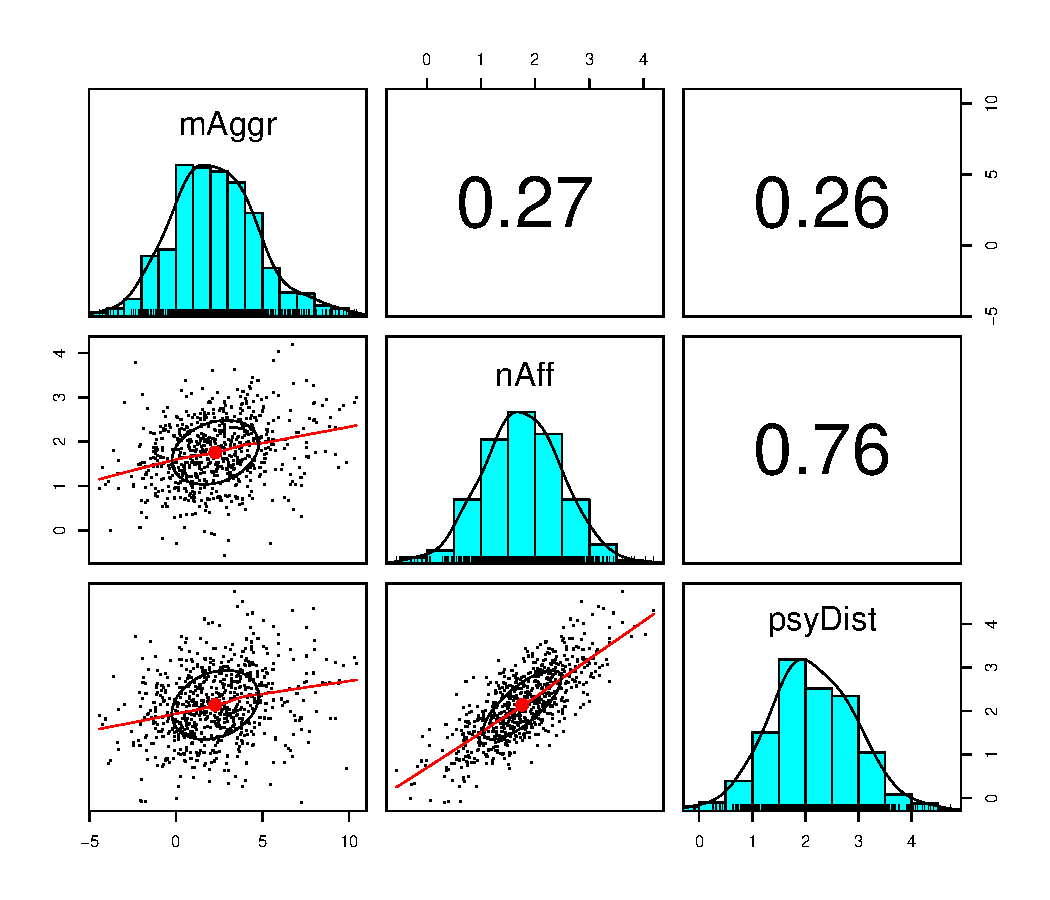
\includegraphics{ReCenterPsychStats_files/figure-latex/unnamed-chunk-27-1.pdf}

What do we observe?

\begin{itemize}
\tightlist
\item
  All 3 variables look normally distributed
\item
  The relationship between mAggr with nAff and psyDist is quite comparable
\item
  The relationship between nAff and psyDist is very strong
\item
  Are these correlations significant? Revelle \citeyearpar{revelle_introduction_2021} is not a fan of the associated \emph{p} value, but we can get it several ways (hang tight).
\end{itemize}

Writing up an APA style results section frequently involves tables. A helpful package for doing this is \emph{apaTables}. An instructional article notes the contributions of tools like this contributing to the \emph{reproducibility} of science by reducing errors made when the author or analyst retypes or copies text from output to the manuscript. When the R script is shared through an open science framework, reproducibility is further enhanced \citep{stanley_reproducible_2018}.

We pass our tiny df to the \emph{apa.cor.table()} function of the \emph{apaTables} package. Commands allow us to specify what is included in the table and whether it should be displayed in the console or saved as a document to the project's folder.

\begin{Shaded}
\begin{Highlighting}[]
\CommentTok{\# unlike the psych package, this function removes any categorical}
\CommentTok{\# variables}
\NormalTok{Table1\_Cor }\OtherTok{\textless{}{-}}\NormalTok{ apaTables}\SpecialCharTok{::}\FunctionTok{apa.cor.table}\NormalTok{(tiny\_df, }\AttributeTok{filename =} \StringTok{"Table1\_Cor.doc"}\NormalTok{,}
    \AttributeTok{table.number =} \DecValTok{1}\NormalTok{, }\AttributeTok{show.conf.interval =} \ConstantTok{FALSE}\NormalTok{, }\AttributeTok{landscape =} \ConstantTok{TRUE}\NormalTok{)}
\end{Highlighting}
\end{Shaded}

\begin{verbatim}
The ability to suppress reporting of reporting confidence intervals has been deprecated in this version.
The function argument show.conf.interval will be removed in a later version.
\end{verbatim}

\begin{Shaded}
\begin{Highlighting}[]
\CommentTok{\# swap in this command to see it in the console}
\FunctionTok{print}\NormalTok{(Table1\_Cor)}
\end{Highlighting}
\end{Shaded}

\begin{verbatim}

Table 1 

Means, standard deviations, and correlations with confidence intervals
 

  Variable   M    SD   1          2         
  1. mAggr   2.27 2.51                      
                                            
  2. nAff    1.76 0.72 .27**                
                       [.20, .33]           
                                            
  3. psyDist 2.14 0.80 .26**      .76**     
                       [.19, .32] [.73, .79]
                                            

Note. M and SD are used to represent mean and standard deviation, respectively.
Values in square brackets indicate the 95% confidence interval.
The confidence interval is a plausible range of population correlations 
that could have caused the sample correlation (Cumming, 2014).
 * indicates p < .05. ** indicates p < .01.
 
\end{verbatim}

These types of statistics are often presented in the preliminary results portion of an empirical manuscript. Here is how I might write them up.

\hypertarget{results}{%
\section{Results}\label{results}}

Our sample included Asian American (\emph{n} = 398), Latinx (\emph{n} = 182), and Black (\emph{n} = 133) participants. Visual inspection of the three variables of interest (negative affect, psychological distress, microaggressions) combined with formal evaluation of skewness and kurtosis suggested univariate normality. Correlations between negative affect and psychological distress were quite strong; correlations with each of these variables and microaggressions were moderate. Results are presented in Table 1.

\hypertarget{practice-problems}{%
\section{Practice Problems}\label{practice-problems}}

The three exercises described below are designed to ``meet you where you are'' and allow you to challenge your skills depending on your comfort with statistics and R.

Regardless which you choose, you should:

\begin{itemize}
\tightlist
\item
  Create a tiny\_df from a larger df
\item
  Calculate and interpret descriptives for the continuously scaled variables
\item
  Create the SPLOM (pairs.panels) of the continuously scaled variables
\item
  Use the \emph{apaTables} package to make an APA style table with means, standard deviations, and correlations
\item
  Write up a mini-results section (APA style)
\end{itemize}

\hypertarget{problem-1-change-the-random-seed}{%
\subsection{Problem \#1: Change the Random Seed}\label{problem-1-change-the-random-seed}}

If this topic feels a bit overwhelming, simply change the random seed in the data simulation (at the very top), then rework the lesson exactly as written. This should provide minor changes to the data (maybe in the second or third decimal point), but the results will likely be very similar.

\hypertarget{problem-2-swap-variables-in-the-simulation}{%
\subsection{Problem \#2: Swap Variables in the Simulation}\label{problem-2-swap-variables-in-the-simulation}}

Use the simulated data from the Lui \citeyearpar{lui_racial_2020} study. However, select three continuous variables (2 must be different from mine) and then conduct the analyses.

\hypertarget{problem-3-use-or-simulate-your-own-data}{%
\subsection{Problem \#3: Use (or Simulate) Your Own Data}\label{problem-3-use-or-simulate-your-own-data}}

Use data for which you have permission and access. This could be IRB approved data you have collected or from your lab; data you simulate from a published article; data from an open science repository; or data from other chapters in this OER.

\hypertarget{grading-rubric}{%
\subsection{Grading Rubric}\label{grading-rubric}}

Regardless which option(s) you chose, use the elements in the grading rubric to guide you through the practice.

\begin{longtable}[]{@{}
  >{\raggedright\arraybackslash}p{(\columnwidth - 4\tabcolsep) * \real{0.5775}}
  >{\centering\arraybackslash}p{(\columnwidth - 4\tabcolsep) * \real{0.2113}}
  >{\raggedright\arraybackslash}p{(\columnwidth - 4\tabcolsep) * \real{0.2113}}@{}}
\toprule
\begin{minipage}[b]{\linewidth}\raggedright
Element
\end{minipage} & \begin{minipage}[b]{\linewidth}\centering
Points Poss
\end{minipage} & \begin{minipage}[b]{\linewidth}\raggedright
Points Earned
\end{minipage} \\
\midrule
\endhead
1. Create the tiny\_df & 3 & \\
2. Descriptives of tiny\_df & 3 & \\
3. SPLOM/pairs.panels & 3 & \\
4. apaTables matrix & 3 & \\
5. Mini-results & 5 & \\
6. Explanation/discussion with a grader & 5 & \\
**Totals & 22 & \\
\bottomrule
\end{longtable}

\hypertarget{oneway}{%
\chapter{One-way ANOVA}\label{oneway}}

\href{https://spu.hosted.panopto.com/Panopto/Pages/Viewer.aspx?pid=c88f8492-0599-462d-a471-ad8a01702156}{Screencasted Lecture Link}

One-way ANOVA allows the researcher to analyze mean differences between two or more groups on a between-subjects factor. For the one-way ANOVA, each case (i.e., individual, participant) must have scores on two variables: a factor and a dependent variable.

The factor must be categorical in nature, dividing the cases into two or more groups or levels. These levels could be ordered (e.g., placebo, low dose, high dose) or unordered (e.g., cognitive-behavioral, existential, psychodynamic). The dependent variable must be assessed on a quantitative, continuous dimension. The ANOVA \emph{F} test evaluates whether population means on the dependent variable differ across the levels of the factor.

One-way ANOVA can be used in experimental, quasi-experimental, and field studies. As we work through the chapter, we will examine some some of the requirements (assumptions) of the statistic in greater detail.

\hypertarget{navigating-this-lesson-2}{%
\section{Navigating this Lesson}\label{navigating-this-lesson-2}}

There is about 2 hours of lecture. If you work through the materials with me, plan for another two hours of study.

\hypertarget{learning-objectives-2}{%
\subsection{Learning Objectives}\label{learning-objectives-2}}

Learning objectives from this lecture include the following:

\begin{itemize}
\tightlist
\item
  Evaluate the statistical assumptions associated with one-way analysis of variance (ANOVA).
\item
  Describe the relationship between model/between-subjects and residual/within-subjects variance.
\item
  Narrate the steps in conducting a formal one-way ANOVA beginning with testing the statistical assumptions through writing up an APA style results section.
\item
  Conduct a one-way ANOVA in R (including calculation of effect sizes and follow-up to the omnibus).
\item
  Conduct a power analysis for a one-way ANOVA.
\item
  Produce an APA style results section.
\end{itemize}

\hypertarget{planning-for-practice-1}{%
\subsection{Planning for Practice}\label{planning-for-practice-1}}

In each of these lessons I provide suggestions for practice that allow you to select one or more problems that are graded in difficulty. The least complex is to change the random seed and rework the problem demonstrated in the lesson. The results \emph{should} map onto the ones obtained in the lecture.

The second option comes from the research vignette. The Tran et al. \citeyearpar{tran_you_2014} vignette has two variables where the authors have conducted one-way ANOVAs. I will demonstrate one (\emph{Accurate}) in this lecture; the second is available as one of the homework options.

As a third option, you are welcome to use data to which you have access and is suitable for two-way ANOVA. In either case the practice options suggest that you:

\begin{itemize}
\tightlist
\item
  test the statistical assumptions
\item
  conduct a one-way ANOVA, including

  \begin{itemize}
  \tightlist
  \item
    omnibus test and effect size
  \item
    follow-up (pairwise, planned comparisons, polynomial trends)
  \end{itemize}
\item
  write a results section to include a figure and tables
\end{itemize}

\hypertarget{readings-resources-1}{%
\subsection{Readings \& Resources}\label{readings-resources-1}}

In preparing this chapter, I drew heavily from the following resource(s) that are freely available on the internet. Other resources are cited (when possible, linked) in the text with complete citations in the reference list.

\begin{itemize}
\tightlist
\item
  Navarro, D. (2020). Chapter 14: Comparing Several Means (one-Way ANOVA). In \href{https://learningstatisticswithr.com/}{Learning Statistics with R - A tutorial for Psychology Students and other Beginners}. Retrieved from \url{https://stats.libretexts.org/Bookshelves/Applied_Statistics/Book\%3A_Learning_Statistics_with_R_-_A_tutorial_for_Psychology_Students_and_other_Beginners_(Navarro)}

  \begin{itemize}
  \tightlist
  \item
    Navarro's OER includes a good mix of conceptual information about one-way ANOVA as well as R code. My code/approach is a mix of Green and Salkind's \citeyearpar{green_using_2014}, Field's \citeyearpar{field_discovering_2012}, Navarro's \citeyearpar{navarro_chapter_2020}, and other techniques I have found on the internet and learned from my students.
  \end{itemize}
\item
  Crump, M. J. C. (2018). Chapter 5.5.2, Simulating data for one-way between subjects design with 3 levels. In \href{https://crumplab.github.io/programmingforpsych/simulating-and-analyzing-data-in-r.html\#single-factor-anovas-data-simulation-and-analysis}{Programming for Psychologists: Data Creation and Analysis}. Retrieved from \url{https://crumplab.github.io/programmingforpsych/simulating-and-analyzing-data-in-r.html\#single-factor-anovas-data-simulation-and-analysis}

  \begin{itemize}
  \tightlist
  \item
    Although this reference is on simulating data, the process of simulation can provide another perspective on one-way ANOVA.
  \end{itemize}
\item
  Tran, A. G. T. T., \& Lee, R. M. (2014). You speak English well! Asian Americans' reactions to an exceptionalizing stereotype. \emph{Journal of Counseling Psychology, 61}(3), 484--490. \url{https://doi.org/10.1037/cou0000034}

  \begin{itemize}
  \tightlist
  \item
    The source of our research vignette.
  \end{itemize}
\end{itemize}

\hypertarget{packages}{%
\subsection{Packages}\label{packages}}

The packages used in this lesson are embedded in this code. When the hashtags are removed, the script below will (a) check to see if the following packages are installed on your computer and, if not (b) install them.

\begin{Shaded}
\begin{Highlighting}[]
\CommentTok{\# will install the package if not already installed easy plotting for}
\CommentTok{\# simple ANOVA if(!require(gplots))\{install.packages(\textquotesingle{}gplots\textquotesingle{})\}}
\CommentTok{\# creating new variables and other handy functions}
\CommentTok{\# if(!require(tidyverse))\{install.packages(\textquotesingle{}tidyverse\textquotesingle{})\} a specific}
\CommentTok{\# part of the tidyverse with useful tools for manipulating data}
\CommentTok{\# if(!require(dplyr))\{install.packages(\textquotesingle{}dplyr\textquotesingle{})\} for descriptive}
\CommentTok{\# statistics and writing them as csv files}
\CommentTok{\# if(!require(psych))\{install.packages(\textquotesingle{}psych\textquotesingle{})\} a number of wrappers}
\CommentTok{\# for ANOVA models; today for evaluating the Shapiro}
\CommentTok{\# if(!require(rstatix))\{install.packages(\textquotesingle{}rstatix\textquotesingle{})\} produces effect}
\CommentTok{\# sizes if(!require(lsr))\{install.packages(\textquotesingle{}lsr\textquotesingle{})\} estimating sample}
\CommentTok{\# sizes and power analysis if(!require(pwr))\{install.packages(\textquotesingle{}pwr\textquotesingle{})\}}
\CommentTok{\# produces an APA style table for ANOVAs and other models}
\CommentTok{\# if(!require(apaTAbles))\{install.packages(\textquotesingle{}apaTables\textquotesingle{})\} helps with}
\CommentTok{\# formats like decimals and percentages for inline code}
\CommentTok{\# if(!require(formattable))\{install.packages(\textquotesingle{}formattable\textquotesingle{})\} more}
\CommentTok{\# effect size options}
\CommentTok{\# if(!require(effectsize))\{install.packages(\textquotesingle{}effectsize\textquotesingle{})\}}
\end{Highlighting}
\end{Shaded}

\hypertarget{workflow-for-one-way-anova}{%
\section{Workflow for One-Way ANOVA}\label{workflow-for-one-way-anova}}

The following is a proposed workflow for conducting a one-way ANOVA.

\begin{figure}
\centering
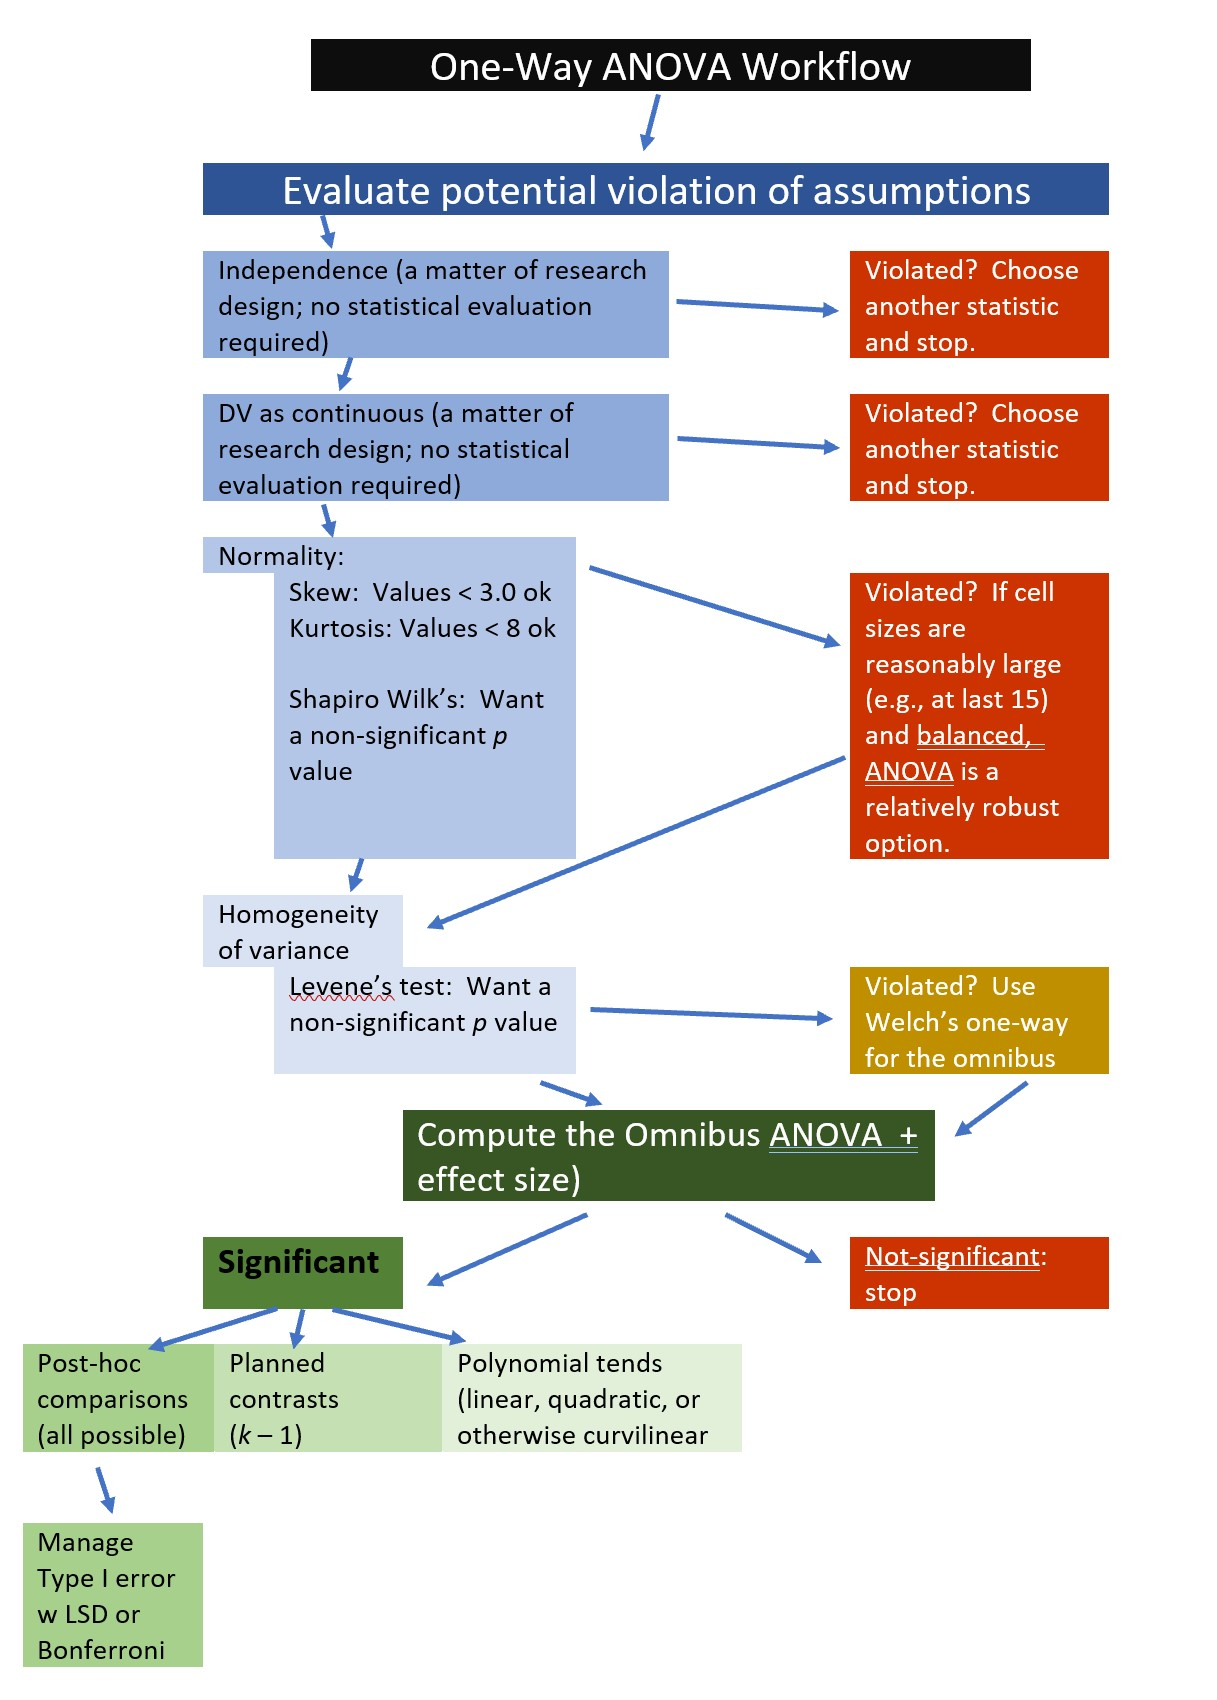
\includegraphics{images/oneway/OnewayWrkFlw.jpg}
\caption{A colorful image of a workflow for the one-way ANOVA}
\end{figure}

\begin{enumerate}
\def\labelenumi{\arabic{enumi}.}
\tightlist
\item
  Prepare (upload) data.
\item
  Explore data

  \begin{itemize}
  \tightlist
  \item
    graphs
  \item
    descriptive statistics
  \end{itemize}
\item
  Checking distributional assumptions

  \begin{itemize}
  \tightlist
  \item
    assessing normality via skew, kurtosis, Shapiro Wilks
  \item
    checking for violation of homogeneity of variance assumption with Levene's test; if we violate this we can use Welch's omnibus ANOVA
  \end{itemize}
\item
  Compute the omnibus ANOVA (remember to use Welch's if Levene's \emph{p} \textless{} .05)
\item
  Compute post-hoc comparisons, planned contrasts, or polynomial trends
\item
  Managing Type I error
\item
  Sample size/power analysis (which you should think about first -- but in the context of teaching ANOVA, it's more pedagogically sensible, here)
\end{enumerate}

\hypertarget{research-vignette-1}{%
\section{Research Vignette}\label{research-vignette-1}}

The \emph{exceptionalizing racial stereotype} is microaggression framed as interpersonally complimentary, but perpetuates negative stereotypical views of a racial/ethnic group. We are using data that is \emph{simulated} from a random clinical trial (RCT) conducted by Tran and Lee \citeyearpar{tran_you_2014}.

The one-way ANOVA examples we are simulating represent the post-only design which investigated three levels of the exceptionalizing stereotype in a sample of Asian American participants. This experimental design involved a confederate (posing as a peer) whose parting comment fell into the low racial loading, high racial loading, or control conditions.

\begin{longtable}[]{@{}
  >{\raggedright\arraybackslash}p{(\columnwidth - 6\tabcolsep) * \real{0.2388}}
  >{\raggedright\arraybackslash}p{(\columnwidth - 6\tabcolsep) * \real{0.1791}}
  >{\raggedright\arraybackslash}p{(\columnwidth - 6\tabcolsep) * \real{0.2687}}
  >{\raggedright\arraybackslash}p{(\columnwidth - 6\tabcolsep) * \real{0.3134}}@{}}
\toprule
\begin{minipage}[b]{\linewidth}\raggedright
COND
\end{minipage} & \begin{minipage}[b]{\linewidth}\raggedright
Assignment
\end{minipage} & \begin{minipage}[b]{\linewidth}\raggedright
Manipulation
\end{minipage} & \begin{minipage}[b]{\linewidth}\raggedright
Post-test Observation
\end{minipage} \\
\midrule
\endhead
\textbf{Low} racial loading condition (\emph{n} = 22) & Random & Yes: ``Nice talking to you. You speak English well.'' & \textbf{Accurate} \\
\textbf{High} racial loading (\emph{n} = 23) & Random & Yes: ``Nice talking to you. You speak English well for an Asian.'' & \textbf{Accurate} \\
\textbf{Control} (\emph{n} = 23) & Random & No: ``Nice talking to you.'' & \textbf{Accurate} \\
\bottomrule
\end{longtable}

Tran and Lee \citeyearpar{tran_you_2014} reported results from two ANOVAs and 4 ANCOVAs, using a pre-test as a covariate. A preprint of their article is available \href{https://pdfs.semanticscholar.org/4146/b528961c041de317c6a4c699f12fc5a4bc22.pdf?_ga=2.179078439.2028716028.1610939782-1660125104.1610939782}{here}.

\begin{itemize}
\tightlist
\item
  \textbf{Accurate} is the DV we will be exploring in this lesson. Participants rated how \emph{accurate} they believed their partner's impression of them was (0 = \emph{very inaccurate}, 3 = \emph{very accurate}).
\item
  \textbf{moreTalk} is the DV suggested as a practice problem. Participants rated how much longer they would continue the interaction with their partner compared to their interactions in general (-2 = \emph{much less than average}, 0 = \emph{average}, 2 = \emph{much more than average}).
\end{itemize}

\hypertarget{data-simulation}{%
\subsection{Data Simulation}\label{data-simulation}}

Simulating data for a one-way ANOVA requires the sample size (rnorm), mean (mean), and standard deviation (sd) for each of the groups \citep{crump_simulating_2018}. In creating this simulation, I used the data from Table 1 in the Tran and Lee \citeyearpar{tran_you_2014} article. Having worked the problem several times, I made one change. The group sizes in the original study were 23, 22, and 23. To increase the probability that we would have statistically significant results in our worked example, I increased the sample sizes to 30 for each group. In this way we have a perfectly \emph{balanced} (equal cell sizes) design.

\begin{Shaded}
\begin{Highlighting}[]
\CommentTok{\# Note, this script results in a different simulation than is in the}
\CommentTok{\# ReadySetR lesson sets a random seed so that we get the same results}
\CommentTok{\# each time}
\FunctionTok{set.seed}\NormalTok{(}\DecValTok{210820}\NormalTok{)}
\CommentTok{\# sample size, M and SD for each group}
\NormalTok{Accurate }\OtherTok{\textless{}{-}} \FunctionTok{c}\NormalTok{(}\FunctionTok{rnorm}\NormalTok{(}\DecValTok{30}\NormalTok{, }\AttributeTok{mean =} \FloatTok{1.18}\NormalTok{, }\AttributeTok{sd =} \FloatTok{0.8}\NormalTok{), }\FunctionTok{rnorm}\NormalTok{(}\DecValTok{30}\NormalTok{, }\AttributeTok{mean =} \FloatTok{1.83}\NormalTok{,}
    \AttributeTok{sd =} \FloatTok{0.58}\NormalTok{), }\FunctionTok{rnorm}\NormalTok{(}\DecValTok{30}\NormalTok{, }\AttributeTok{mean =} \FloatTok{1.76}\NormalTok{, }\AttributeTok{sd =} \FloatTok{0.56}\NormalTok{))}
\CommentTok{\# set upper bound for DV}
\NormalTok{Accurate[Accurate }\SpecialCharTok{\textgreater{}} \DecValTok{3}\NormalTok{] }\OtherTok{\textless{}{-}} \DecValTok{3}
\CommentTok{\# set lower bound for DV}
\NormalTok{Accurate[Accurate }\SpecialCharTok{\textless{}} \DecValTok{0}\NormalTok{] }\OtherTok{\textless{}{-}} \DecValTok{0}
\CommentTok{\# sample size, M and SD for each group}
\NormalTok{moreTalk }\OtherTok{\textless{}{-}} \FunctionTok{c}\NormalTok{(}\FunctionTok{rnorm}\NormalTok{(}\DecValTok{30}\NormalTok{, }\AttributeTok{mean =} \SpecialCharTok{{-}}\FloatTok{0.82}\NormalTok{, }\AttributeTok{sd =} \FloatTok{0.91}\NormalTok{), }\FunctionTok{rnorm}\NormalTok{(}\DecValTok{30}\NormalTok{, }\AttributeTok{mean =} \SpecialCharTok{{-}}\FloatTok{0.39}\NormalTok{,}
    \AttributeTok{sd =} \FloatTok{0.66}\NormalTok{), }\FunctionTok{rnorm}\NormalTok{(}\DecValTok{30}\NormalTok{, }\AttributeTok{mean =} \SpecialCharTok{{-}}\FloatTok{0.04}\NormalTok{, }\AttributeTok{sd =} \FloatTok{0.71}\NormalTok{))}
\CommentTok{\# set upper bound for DV}
\NormalTok{moreTalk[moreTalk }\SpecialCharTok{\textgreater{}} \DecValTok{2}\NormalTok{] }\OtherTok{\textless{}{-}} \DecValTok{2}
\CommentTok{\# set lower bound for DV}
\NormalTok{moreTalk[moreTalk }\OtherTok{\textless{}{-}} \DecValTok{2}\NormalTok{] }\OtherTok{\textless{}{-}} \SpecialCharTok{{-}}\DecValTok{2}
\CommentTok{\# IDs for participants}
\NormalTok{ID }\OtherTok{\textless{}{-}} \FunctionTok{factor}\NormalTok{(}\FunctionTok{seq}\NormalTok{(}\DecValTok{1}\NormalTok{, }\DecValTok{90}\NormalTok{))}
\CommentTok{\# name factors and identify how many in each group; should be in same}
\CommentTok{\# order as first row of script}
\NormalTok{COND }\OtherTok{\textless{}{-}} \FunctionTok{c}\NormalTok{(}\FunctionTok{rep}\NormalTok{(}\StringTok{"High"}\NormalTok{, }\DecValTok{30}\NormalTok{), }\FunctionTok{rep}\NormalTok{(}\StringTok{"Low"}\NormalTok{, }\DecValTok{30}\NormalTok{), }\FunctionTok{rep}\NormalTok{(}\StringTok{"Control"}\NormalTok{, }\DecValTok{30}\NormalTok{))}
\CommentTok{\# groups the 3 variables into a single df: ID\#, DV, condition}
\NormalTok{accSIM30 }\OtherTok{\textless{}{-}} \FunctionTok{data.frame}\NormalTok{(ID, COND, Accurate, moreTalk)}
\end{Highlighting}
\end{Shaded}

\hypertarget{working-the-problem}{%
\section{Working the Problem}\label{working-the-problem}}

\hypertarget{preparing-the-data}{%
\subsection{Preparing the Data}\label{preparing-the-data}}

Examining the data is important for several reasons. First, we can begin to inspect for any anomalies. Second, if we are confused about what statistic we wish to apply, understanding the characteristics of the data can provide clues.

In R markdown we can

\begin{itemize}
\tightlist
\item
  look at the data by clicking on it, and
\item
  examine its structure with the \emph{str()} function.
\end{itemize}

Let's do both.

\begin{Shaded}
\begin{Highlighting}[]
\FunctionTok{str}\NormalTok{(accSIM30)}
\end{Highlighting}
\end{Shaded}

\begin{verbatim}
'data.frame':   90 obs. of  4 variables:
 $ ID      : Factor w/ 90 levels "1","2","3","4",..: 1 2 3 4 5 6 7 8 9 10 ...
 $ COND    : chr  "High" "High" "High" "High" ...
 $ Accurate: num  0.42 1.123 0.885 1.569 1.831 ...
 $ moreTalk: num  -0.64 -2 -0.25 0.146 -0.996 ...
\end{verbatim}

If we look at this simple dataset, we see that we see that

\begin{itemize}
\tightlist
\item
  \textbf{COND} is a grouping variable) with 3 levels (high, low, control)

  \begin{itemize}
  \tightlist
  \item
    it is presently in ``chr'' (character) format, it needs to be changed to be a factor.
  \end{itemize}
\item
  \textbf{Accurate} is a continuous variable

  \begin{itemize}
  \tightlist
  \item
    it is presently in ``num'' (numerical) format, this is an appropriate format.
  \end{itemize}
\item
  \textbf{moreTalk} is a continuous variable

  \begin{itemize}
  \tightlist
  \item
    it is presently in ``num'' (numerical) format, this is an appropriate format
  \end{itemize}
\end{itemize}

There are many ways to convert variables to factors; here is one of the simplest.

\begin{Shaded}
\begin{Highlighting}[]
\CommentTok{\#convert variable to factor}
\NormalTok{accSIM30}\SpecialCharTok{$}\NormalTok{COND }\OtherTok{\textless{}{-}} \FunctionTok{factor}\NormalTok{(accSIM30}\SpecialCharTok{$}\NormalTok{COND)}
\end{Highlighting}
\end{Shaded}

Let's recheck the structure

\begin{Shaded}
\begin{Highlighting}[]
\FunctionTok{str}\NormalTok{(accSIM30)}
\end{Highlighting}
\end{Shaded}

\begin{verbatim}
'data.frame':   90 obs. of  4 variables:
 $ ID      : Factor w/ 90 levels "1","2","3","4",..: 1 2 3 4 5 6 7 8 9 10 ...
 $ COND    : Factor w/ 3 levels "Control","High",..: 2 2 2 2 2 2 2 2 2 2 ...
 $ Accurate: num  0.42 1.123 0.885 1.569 1.831 ...
 $ moreTalk: num  -0.64 -2 -0.25 0.146 -0.996 ...
\end{verbatim}

By default, R orders factors alphabetically. This means, analyses will assume that ``Control'' (C) is the lowest condition, then ``High,'' then ``Low.'' Since these have theoretically ordered values, we want them in the order of ``Control,'' ``Low,'' ``High.''

Here is the script to create an ordered factor. The order in which the variables are entered in the concatenated list (``c'') establishes the order (e.g., levels).

\begin{Shaded}
\begin{Highlighting}[]
\CommentTok{\# ordering the factor}
\NormalTok{accSIM30}\SpecialCharTok{$}\NormalTok{COND }\OtherTok{\textless{}{-}} \FunctionTok{factor}\NormalTok{(accSIM30}\SpecialCharTok{$}\NormalTok{COND, }\AttributeTok{levels =} \FunctionTok{c}\NormalTok{(}\StringTok{"Control"}\NormalTok{, }\StringTok{"Low"}\NormalTok{, }\StringTok{"High"}\NormalTok{))}
\end{Highlighting}
\end{Shaded}

Again, we can check our work.

\begin{Shaded}
\begin{Highlighting}[]
\CommentTok{\#another structure check}
\FunctionTok{str}\NormalTok{(accSIM30)}
\end{Highlighting}
\end{Shaded}

\begin{verbatim}
'data.frame':   90 obs. of  4 variables:
 $ ID      : Factor w/ 90 levels "1","2","3","4",..: 1 2 3 4 5 6 7 8 9 10 ...
 $ COND    : Factor w/ 3 levels "Control","Low",..: 3 3 3 3 3 3 3 3 3 3 ...
 $ Accurate: num  0.42 1.123 0.885 1.569 1.831 ...
 $ moreTalk: num  -0.64 -2 -0.25 0.146 -0.996 ...
\end{verbatim}

Now our variables are suitable for analysis.

At this point, you may wish to export and/or import the data as a .csv (think ``Excel lite'') or .rds (R object that preserves the information about the variables -- such changing COND to an ordered factor), here is the code to do so. The data should save in the same folder as the .rmd file. Therefore, it is really important (think, ``good R hygiene'') to have organized your folders so that your .rmd and data files are co-located.

I have hashtagged out the code. If you wish to use it, delete the hashtags. Although I show the .csv code first, my personal preference is to save R data as .rds files. While they aren't easy to ``see'' as an independent file, they retain the formatting of the variables. For a demonstration, refer back to the \protect\hyperlink{Ready}{Ready\_Set\_R} lesson.

\begin{Shaded}
\begin{Highlighting}[]
\CommentTok{\# write the simulated data as a .csv write.table(accSIM30,}
\CommentTok{\# file=\textquotesingle{}accSIM.csv\textquotesingle{}, sep=\textquotesingle{},\textquotesingle{}, col.names=TRUE, row.names=FALSE) bring}
\CommentTok{\# back the simulated dat from a .csv file acc\_csv \textless{}{-} read.csv}
\CommentTok{\# (\textquotesingle{}accSIM.csv\textquotesingle{}, header = TRUE)}
\end{Highlighting}
\end{Shaded}

\begin{Shaded}
\begin{Highlighting}[]
\CommentTok{\# a quick demo to show that the .csv format loses the variable}
\CommentTok{\# formatting str(acc\_csv)}
\end{Highlighting}
\end{Shaded}

\begin{Shaded}
\begin{Highlighting}[]
\CommentTok{\# to save the df as an .rds (think \textquotesingle{}R object\textquotesingle{}) file on your computer;}
\CommentTok{\# it should save in the same file as the .rmd file you are working}
\CommentTok{\# with saveRDS(accSIM30, \textquotesingle{}accSIM.rds\textquotesingle{}) bring back the simulated dat}
\CommentTok{\# from an .rds file acc\_RDS \textless{}{-} readRDS(\textquotesingle{}accSIM.rds\textquotesingle{})}
\end{Highlighting}
\end{Shaded}

\begin{Shaded}
\begin{Highlighting}[]
\CommentTok{\# a quick demo to show that the .rds format preserves the variable}
\CommentTok{\# formatting str(acc\_RDS)}
\end{Highlighting}
\end{Shaded}

Note that I renamed each of these data objects to reflect the form in whic I saved them (i.e., ``acc\_csv'', ``acc\_RDS''). If you have followed this step, you will want to rename the file before continuing with the rest of the chapter. Alternatively, you can start from scratch, re-run the code to simulate the data, and skip this portion on importing/exporting data.

\begin{Shaded}
\begin{Highlighting}[]
\CommentTok{\#accSIM30 \textless{}{-} acc\_RDS}
\CommentTok{\#or}
\CommentTok{\#accSIM30 \textless{}{-} acc\_csv}
\end{Highlighting}
\end{Shaded}

\hypertarget{exploring-the-distributional-characteristics-numerically}{%
\subsection{Exploring the Distributional Characteristics Numerically}\label{exploring-the-distributional-characteristics-numerically}}

We will explore the data such that you will have several tools for future exploration. In this first demonstration I will quickly produce a mean and standard deviation.

These functions are in base R. The \emph{aggregate()} function lets R know we want output by a grouping variable. We then list the variable of interest, a tilda (I think of the word ``by''), and then the grouping variable (I think ``Accurate by COND''). Finally we list the dataframe and the statistic (e.g., mean or standard deviation). R is case sensitive to check your capitalization if your code fails to execute.

\begin{Shaded}
\begin{Highlighting}[]
\FunctionTok{aggregate}\NormalTok{(Accurate }\SpecialCharTok{\textasciitilde{}}\NormalTok{ COND, accSIM30, mean)}
\end{Highlighting}
\end{Shaded}

\begin{verbatim}
     COND Accurate
1 Control 1.756195
2     Low 1.900116
3    High 1.152815
\end{verbatim}

\begin{Shaded}
\begin{Highlighting}[]
\FunctionTok{aggregate}\NormalTok{(Accurate }\SpecialCharTok{\textasciitilde{}}\NormalTok{ COND, accSIM30, sd)}
\end{Highlighting}
\end{Shaded}

\begin{verbatim}
     COND  Accurate
1 Control 0.4603964
2     Low 0.6301138
3    High 0.6587486
\end{verbatim}

Before looking at graphs, we can see that racially loaded \emph{high} condition has the lowest accuracy score and the largest variability. Let's produce some helpful figures so that we can visualize this.

\hypertarget{exploring-the-distributional-characteristics-graphically}{%
\subsection{Exploring the Distributional Characteristics Graphically}\label{exploring-the-distributional-characteristics-graphically}}

The package \emph{gplots} produces a simple line graph and the script is fairly intuitive. The \emph{plotmeans()} function plots the means with error bars (95\% confidence intervals) around the mean. Regarding the confidence intervals, we can think, ``How confident are we that the mean is this particular value?'' Earlier we noted that the ``high racial loading condition'' had the lowest mean and the widest variability. Is this apparent from the graph?

\begin{Shaded}
\begin{Highlighting}[]
\CommentTok{\# plots DV by IV}
\NormalTok{gplots}\SpecialCharTok{::}\FunctionTok{plotmeans}\NormalTok{(}\AttributeTok{formula =}\NormalTok{ Accurate }\SpecialCharTok{\textasciitilde{}}\NormalTok{ COND, }\AttributeTok{data =}\NormalTok{ accSIM30, }\AttributeTok{xlab =} \StringTok{"Racial Loading Condition"}\NormalTok{,}
    \AttributeTok{ylab =} \StringTok{"Accuracy of Confederate\textquotesingle{}s Impression"}\NormalTok{, }\AttributeTok{n.label =} \ConstantTok{TRUE}\NormalTok{)}
\end{Highlighting}
\end{Shaded}

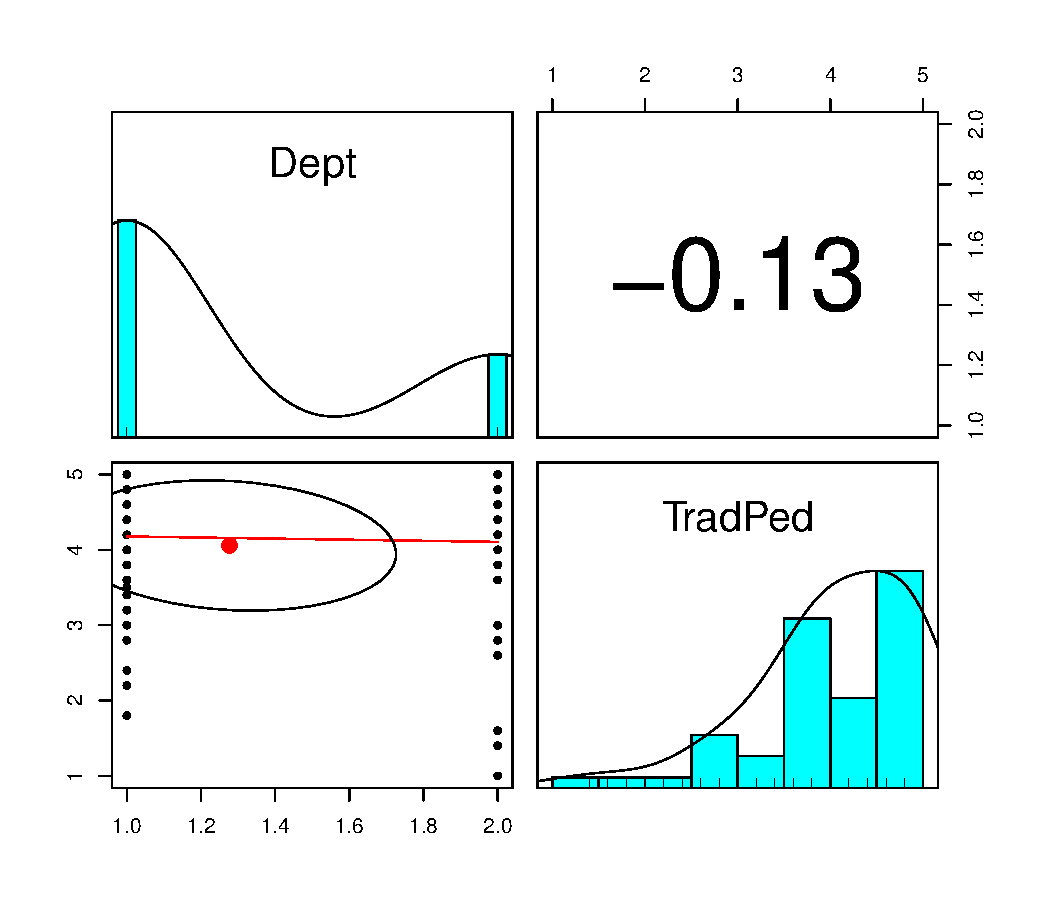
\includegraphics{ReCenterPsychStats_files/figure-latex/unnamed-chunk-43-1.pdf}

\begin{Shaded}
\begin{Highlighting}[]
\CommentTok{\# this code could be more elegantly written in one row plotmeans}
\CommentTok{\# (formula = Accurate \textasciitilde{} COND, data = accSIM30, xlab = \textquotesingle{}Racial Loading}
\CommentTok{\# Condition\textquotesingle{}, ylab = \textquotesingle{}Accuracy of Confederate\textquotesingle{}s Impression\textquotesingle{}, n.label}
\CommentTok{\# = TRUE)}
\end{Highlighting}
\end{Shaded}

Boxplots, with the \emph{boxplot2()} function provide another view of our data. In boxplots the center value is the median. The box spans the \emph{interquartile range} and ranges from the 25th to the 75th percentile. The whiskers cover 1.5 times the interquartile range. When this does not capture the entire range, outliers are represented with dots.

\begin{Shaded}
\begin{Highlighting}[]
\NormalTok{gplots}\SpecialCharTok{::}\FunctionTok{boxplot2}\NormalTok{(Accurate }\SpecialCharTok{\textasciitilde{}}\NormalTok{ COND, }\AttributeTok{data =}\NormalTok{ accSIM30, }\AttributeTok{xlab =} \StringTok{"Racial Loading Condition"}\NormalTok{,}
    \AttributeTok{ylab =} \StringTok{"Accuracy of Confederate\textquotesingle{}s Impression"}\NormalTok{, }\AttributeTok{n.label =} \ConstantTok{TRUE}\NormalTok{)}
\end{Highlighting}
\end{Shaded}

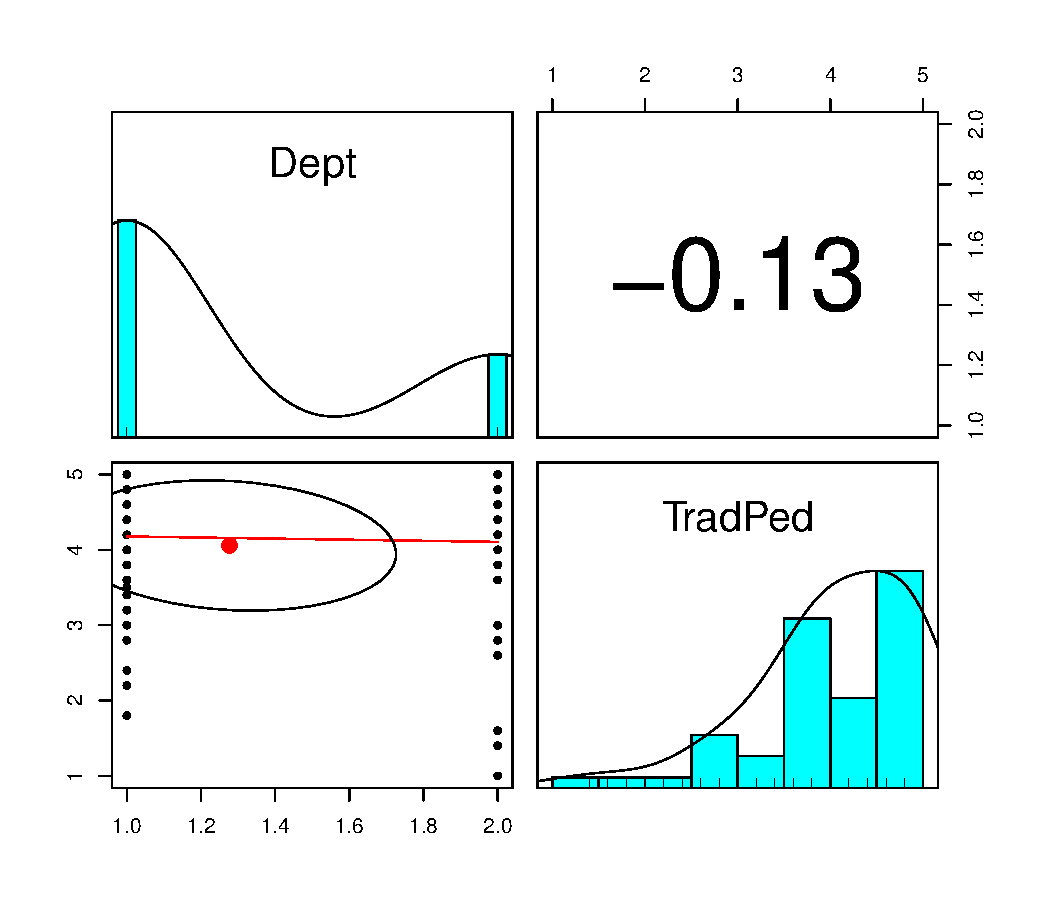
\includegraphics{ReCenterPsychStats_files/figure-latex/unnamed-chunk-44-1.pdf}

From both the boxplot and the linegraph with error bars, we can see that participants in the low racial loading condition have the highest accuracy ratings. This is followed by the control and then high racial loading conditions. Are these differences statistically significant? This is why we need the one-way ANOVA.

\hypertarget{understanding-anova-with-hand-calculations}{%
\section{\texorpdfstring{Understanding ANOVA with \emph{Hand Calculations}}{Understanding ANOVA with Hand Calculations}}\label{understanding-anova-with-hand-calculations}}

ANOVA was developed by Sir Ronald Fisher in the early 20th century. The name is a bit of a misnomer -- rather than analyzing \emph{variances}, we are investigating differences in \emph{means} (but the formula does take variances into consideration\ldots stay tuned).

ANOVA falls squarely within the tradition of \textbf{null hypothesis significance testing} (NHST). As such, a formal, traditional, ANOVA begins with statements of the null and alternate hypotheses. \emph{Note. In their article, Tran and Lee \citeyearpar{tran_you_2014} do not list such.}

In our example, we would hypothesize that the population means (i.e., Asian or Asian American individuals in the U.S.) are equal:
\[H_{O}: \mu _{1} = \mu _{2} = \mu _{3}\]
There are an number of ways that the \(H_{O}\) could be false. Here are a few:
\[H_{a1}: \mu _{1} \neq \mu _{2} \neq \mu _{3}\]
\[H_{a2}: \mu _{1} = \mu _{2} > \mu _{3}\]
\[H_{a3}: \mu _{1} > \mu _{2} > \mu _{3}\]
The bottom line is that if we have a statistically significant omnibus ANOVA (i.e., the test of the overall significance of the model) and the \(H_{O}\) is false, somewhere between the three levels of the grouping factor, the means are statistically significantly different from each other.

In evaluating the differences between means, one-way ANOVA compares:

\begin{itemize}
\tightlist
\item
  systematic variance to unsystematic variance
\item
  explained to unexplained variation
\item
  experimental effect to the individual differences
\item
  model variance to residual variance
\item
  between group variance to within group variance
\end{itemize}

The ratio of these variances is the \emph{F}-ratio.

Navarro \citeyearpar{navarro_book_2020} offers a set of useful figures to compare between- and within-group variation.

\begin{figure}
\centering
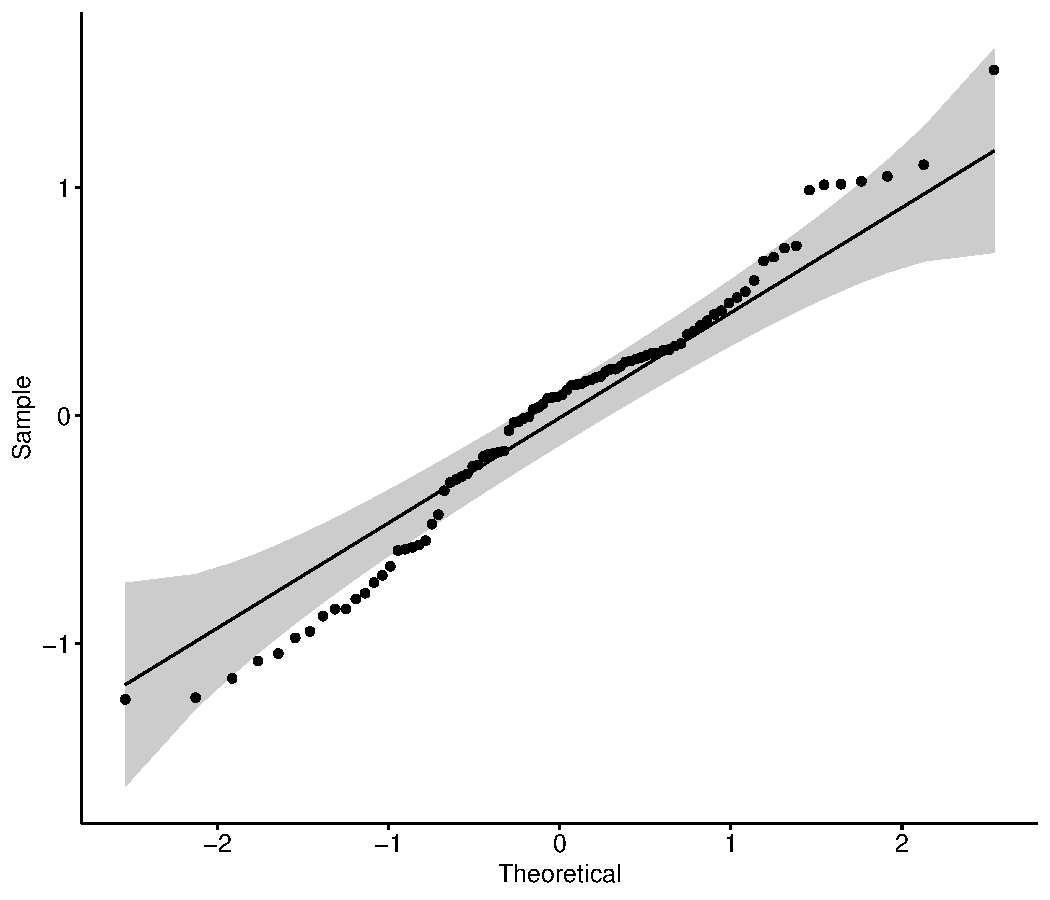
\includegraphics{ReCenterPsychStats_files/figure-latex/unnamed-chunk-45-1.pdf}
\caption{\label{fig:unnamed-chunk-45}Graphical illustration of ``between groups'' variation}
\end{figure}

\begin{figure}
\centering
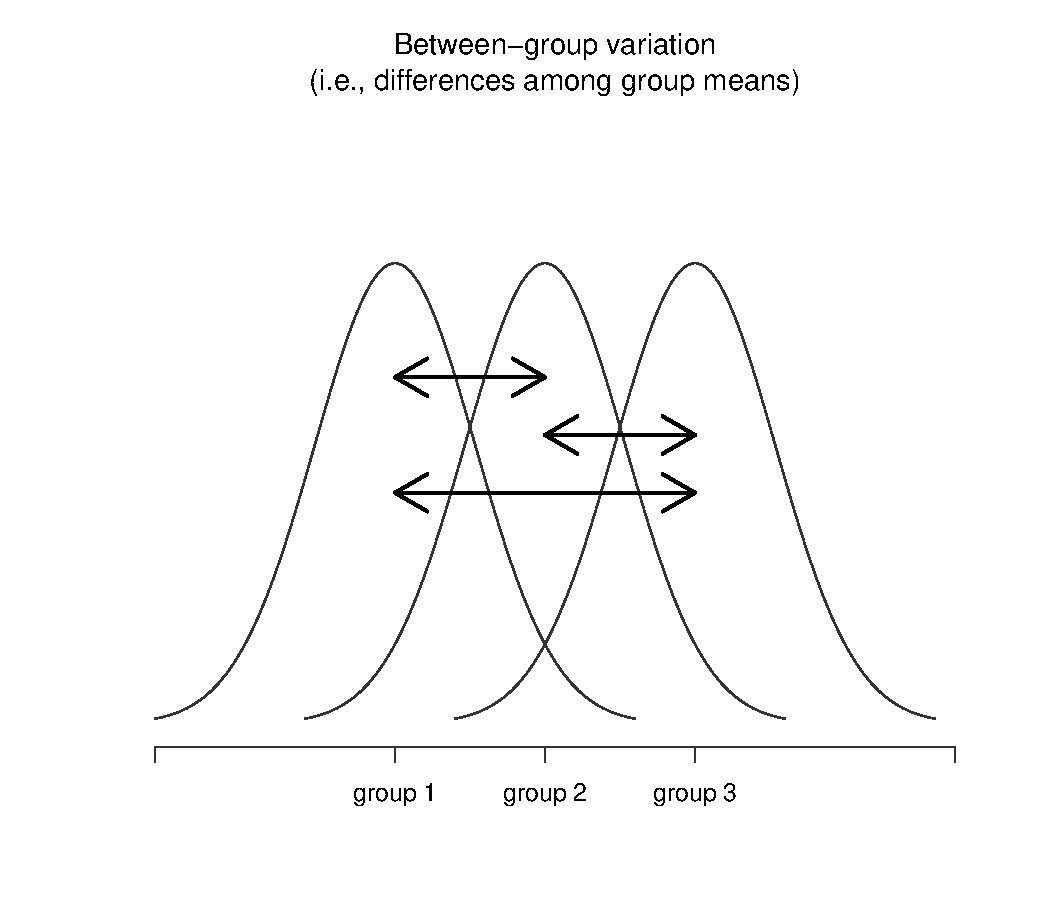
\includegraphics{ReCenterPsychStats_files/figure-latex/unnamed-chunk-46-1.pdf}
\caption{\label{fig:unnamed-chunk-46}Graphical illustration of ``within groups'' variation}
\end{figure}

When between-group variance (i.e,. model variance) is greater than within-group variance (i.e., residual variance) there may be support to suggest that there are statistically significant differences between groups.

Let's examine how variance is partitioned by hand-calculating sums of squares total, model, and residual. Along the way we will use some basic R skills to manipulate the data.

\hypertarget{sums-of-squares-total}{%
\subsection{Sums of Squares Total}\label{sums-of-squares-total}}

Sums of squares total represents the total amount of variance within our data. Examining the formula(s; there are variants of each) can help us gain a conceptual understanding of this.

In this first version of the formula we can see that the grand (or overall) mean is subtracted from each individual score, squared, and then summed. This makes sense: \emph{sums of squares, total}.

\[SS_{T}= \sum (x_{i}-\bar{x}_{grand})^{2}\]
In the next version of the formula we see that the sums of square total is the addition of the sums of squares model and residual.

\[SS_{T}= SS_{M} + SS_{R}\]

``Between'' and ``within'' are another way to understand ``model'' and ``residual.'' This is reflected in the next formula.

\[SS_{T}= SS_{B} + SS_{W}\]
Finally, think of the sums of squares total as the grand variance multiplied by the overall degrees of freedom (\emph{N} - 1).

\[SS_{T}= s_{grand}^{2}(n-1)\]
Let's take a moment to \emph{hand-calculate} \(SS_{T}\). Not to worry -- we'll get R to do the math for us!

Our grand (i.e., overall) mean is

\begin{Shaded}
\begin{Highlighting}[]
\NormalTok{GrandMean }\OtherTok{\textless{}{-}} \FunctionTok{mean}\NormalTok{(accSIM30}\SpecialCharTok{$}\NormalTok{Accurate)}
\NormalTok{GrandMean}
\end{Highlighting}
\end{Shaded}

\begin{verbatim}
[1] 1.603042
\end{verbatim}

Subtracting the grand mean from each Accurate rating yields a mean difference. In the script below I have used the \emph{mutate()} function from the \emph{dplyr} package (a part of the \emph{tidyverse}) to created a new variable ('' m\_dev'') in the dataframe. The \emph{tidyverse} package is one of the few exceptions that I will open via the library. This is because we need it if we are going to use the pipe (\%\textgreater\%) to string parts of our script together.

\begin{Shaded}
\begin{Highlighting}[]
\FunctionTok{library}\NormalTok{(tidyverse)}

\NormalTok{accSIM30 }\OtherTok{\textless{}{-}}\NormalTok{ accSIM30 }\SpecialCharTok{\%\textgreater{}\%} 
\NormalTok{  dplyr}\SpecialCharTok{::}\FunctionTok{mutate}\NormalTok{(}\AttributeTok{m\_dev =}\NormalTok{ Accurate}\SpecialCharTok{{-}}\FunctionTok{mean}\NormalTok{(Accurate))}

\FunctionTok{head}\NormalTok{(accSIM30)}
\end{Highlighting}
\end{Shaded}

\begin{verbatim}
  ID COND  Accurate   moreTalk       m_dev
1  1 High 0.4203896 -0.6398265 -1.18265259
2  2 High 1.1226505 -2.0000000 -0.48039170
3  3 High 0.8852238 -0.2497750 -0.71781837
4  4 High 1.5689439  0.1455637 -0.03409829
5  5 High 1.8307196 -0.9960413  0.22767748
6  6 High 1.8874431 -1.0692978  0.28440098
\end{verbatim}

Pop quiz: What's the sum of our new \emph{m\_dev} variable? Let's check.

\begin{Shaded}
\begin{Highlighting}[]
\FunctionTok{mean}\NormalTok{(accSIM30}\SpecialCharTok{$}\NormalTok{m\_dev)}
\end{Highlighting}
\end{Shaded}

\begin{verbatim}
[1] 0.00000000000000003830065
\end{verbatim}

Unless you run the script at the top of this document (``options(scipen=999)''), R will (seemingly selectively) use \textbf{scientific e notation} to report your results. The proper value is one where the base number (before the ``e'') is multiplied by 10, raised to the power shown: \(3.830065 * 10^{17}\) Another way to think of it is to move the decimal 17 places to the left. In any case, this number is essentially zero.

Back to the point of sums of squares total, the sum of deviations around the grand mean will always be zero. To make them useful, we must square them:

\begin{Shaded}
\begin{Highlighting}[]
\NormalTok{accSIM30 }\OtherTok{\textless{}{-}}\NormalTok{ accSIM30 }\SpecialCharTok{\%\textgreater{}\%} 
\NormalTok{  dplyr}\SpecialCharTok{::}\FunctionTok{mutate}\NormalTok{(}\AttributeTok{m\_devSQ =}\NormalTok{ m\_dev}\SpecialCharTok{\^{}}\DecValTok{2}\NormalTok{)}

\FunctionTok{head}\NormalTok{(accSIM30)}
\end{Highlighting}
\end{Shaded}

\begin{verbatim}
  ID COND  Accurate   moreTalk       m_dev     m_devSQ
1  1 High 0.4203896 -0.6398265 -1.18265259 1.398667144
2  2 High 1.1226505 -2.0000000 -0.48039170 0.230776185
3  3 High 0.8852238 -0.2497750 -0.71781837 0.515263216
4  4 High 1.5689439  0.1455637 -0.03409829 0.001162694
5  5 High 1.8307196 -0.9960413  0.22767748 0.051837034
6  6 High 1.8874431 -1.0692978  0.28440098 0.080883915
\end{verbatim}

If we sum the squared mean deviations we will obtain the total variance (sums of squares total):

\begin{Shaded}
\begin{Highlighting}[]
\NormalTok{SST }\OtherTok{\textless{}{-}} \FunctionTok{sum}\NormalTok{(accSIM30}\SpecialCharTok{$}\NormalTok{m\_devSQ)}
\NormalTok{SST}
\end{Highlighting}
\end{Shaded}

\begin{verbatim}
[1] 39.67818
\end{verbatim}

This value, the sum of squared deviations around the grand mean, is our \(SS_T\). The associated \emph{degrees of freedom} is \(N - 1\); in our case this is 90-1 = 89.

In one-way ANOVA, we divide \(SS_T\) into \textbf{model/between sums of squares} and \textbf{residual/within sums of squares}.

The \emph{model} generally represents the notion that the means are different than each other. We want the variation between our means to be greater than the variation within each of the groups from which our means are calculated.

\hypertarget{sums-of-squares-for-the-model-or-between}{%
\subsection{Sums of Squares for the Model (or Between)}\label{sums-of-squares-for-the-model-or-between}}

We just determined that the total amount of variation within the data is 39.678 units. From this we can estimate how much of this variation our model can explain. \(SS_M\) tells us how much of the total variation can be explained by the fact that different data points come from different groups.

We see this reflected in the formula below, where

\begin{itemize}
\tightlist
\item
  the grand mean is subtracted from each group mean
\item
  this value is squared and multiplied by the number of cases in each group
\item
  these values are summed
\end{itemize}

\[SS_{M}= \sum n_{k}(\bar{x}_{k}-\bar{x}_{grand})^{2}\]

To calculate this, we start with the grand mean (previously calculated): 1.603.

We also estimate the group means.

\begin{Shaded}
\begin{Highlighting}[]
\NormalTok{GroupMeans }\OtherTok{\textless{}{-}} \FunctionTok{aggregate}\NormalTok{(Accurate }\SpecialCharTok{\textasciitilde{}}\NormalTok{ COND, accSIM30, mean)}
\NormalTok{GroupMeans}
\end{Highlighting}
\end{Shaded}

\begin{verbatim}
     COND Accurate
1 Control 1.756195
2     Low 1.900116
3    High 1.152815
\end{verbatim}

This formula occurs in three chunks, representing the control, low, and high racial loading conditions. In each of the chunks we have the \(n\), group mean, and grand mean.

\begin{Shaded}
\begin{Highlighting}[]
\CommentTok{\# Calculated by using object names from our calculations}
\NormalTok{SSM }\OtherTok{\textless{}{-}}\NormalTok{ nControl }\SpecialCharTok{*}\NormalTok{ (ControlMean }\SpecialCharTok{{-}}\NormalTok{ GrandMean)}\SpecialCharTok{\^{}}\DecValTok{2} \SpecialCharTok{+}\NormalTok{ nLow }\SpecialCharTok{*}\NormalTok{ (LowMean }\SpecialCharTok{{-}}\NormalTok{ GrandMean)}\SpecialCharTok{\^{}}\DecValTok{2} \SpecialCharTok{+}
\NormalTok{    nHigh }\SpecialCharTok{*}\NormalTok{ (HighMean }\SpecialCharTok{{-}}\NormalTok{ GrandMean)}\SpecialCharTok{\^{}}\DecValTok{2}
\NormalTok{SSM}
\end{Highlighting}
\end{Shaded}

\begin{verbatim}
[1] 9.432
\end{verbatim}

\begin{Shaded}
\begin{Highlighting}[]
\CommentTok{\# calculated by specifying the actual values from our calculations}
\DecValTok{30} \SpecialCharTok{*}\NormalTok{ (}\FloatTok{1.756} \SpecialCharTok{{-}} \FloatTok{1.603}\NormalTok{)}\SpecialCharTok{\^{}}\DecValTok{2} \SpecialCharTok{+} \DecValTok{30} \SpecialCharTok{*}\NormalTok{ (}\FloatTok{1.9} \SpecialCharTok{{-}} \FloatTok{1.603}\NormalTok{)}\SpecialCharTok{\^{}}\DecValTok{2} \SpecialCharTok{+} \DecValTok{30} \SpecialCharTok{*}\NormalTok{ (}\FloatTok{1.153} \SpecialCharTok{{-}} \FloatTok{1.603}\NormalTok{)}\SpecialCharTok{\^{}}\DecValTok{2}
\end{Highlighting}
\end{Shaded}

\begin{verbatim}
[1] 9.42354
\end{verbatim}

\begin{Shaded}
\begin{Highlighting}[]
\CommentTok{\# Both result in the same}
\end{Highlighting}
\end{Shaded}

This value, \(SS_M\) is the amount of variance accounted for by the model; that is, the the amount of variance accounted for by the grouping variable/factor, COND. Degrees of freedom for \(SS_M\) is always one less than the number of elements (e.g., groups) used in its calculation (\(k-1\)). Because we have three groups, our degrees of freedom for the model is two.

\hypertarget{sums-of-squares-residual-or-within}{%
\subsection{Sums of Squares Residual (or within)}\label{sums-of-squares-residual-or-within}}

To recap, we know there are 39.678 units of variation to be explained in our data. Our model explains 9.432 of these units. Sums of squares residual tells us how much of the variation cannot be explained by the model. This value is influenced by extraneous factors; some will refer to it as ``noise.''

Looking at the formula can assist us in with a conceptual formula. In \(SS_R\) we subtract the group mean from each individual member of the group and then square it.

\[SS_{R}= \sum(x_{ik}-\bar{x}_{k})^{^{2}}\]
Below is another approach to calculating\(SS_R\). In this one the variance for each group is multiplied by its respective degrees of freedom, then summed.

\[SS_{R}= s_{group1}^{2}(n-1) + s_{group2}^{2}(n-1) + s_{group3}^{2}(n-1))\]
Again, the formula is in three chunks -- but this time the calculations are \emph{within-group}. We need the variance (the standard deviation squared) for the calculation.

\begin{Shaded}
\begin{Highlighting}[]
\NormalTok{SDs }\OtherTok{\textless{}{-}} \FunctionTok{aggregate}\NormalTok{ (Accurate }\SpecialCharTok{\textasciitilde{}}\NormalTok{ COND, accSIM30, sd)}
\NormalTok{SDs}
\end{Highlighting}
\end{Shaded}

\begin{verbatim}
     COND  Accurate
1 Control 0.4603964
2     Low 0.6301138
3    High 0.6587486
\end{verbatim}

\hypertarget{on-the-relationship-between-standard-deviation-and-variance}{%
\subsubsection{On the relationship between standard deviation and variance}\label{on-the-relationship-between-standard-deviation-and-variance}}

Early in statistics training the difference between standard deviation (\emph{s} or \(\sigma_{n-1}\)) and variance(\(s^{2}\) or \(\sigma^{2}\)) can be confusing. This calculation demonstrates the relationship between standard deviation and variance. Variance is the standard deviation, squared.

\begin{Shaded}
\begin{Highlighting}[]
\CommentTok{\#when squared, the standard deviation of the control group, }
\CommentTok{\#hould equal the variance reported in the next chunk}
\NormalTok{sdControl}\SpecialCharTok{\^{}}\DecValTok{2}
\end{Highlighting}
\end{Shaded}

\begin{verbatim}
[1] 0.212
\end{verbatim}

\begin{Shaded}
\begin{Highlighting}[]
\NormalTok{VARs }\OtherTok{\textless{}{-}} \FunctionTok{aggregate}\NormalTok{ (Accurate }\SpecialCharTok{\textasciitilde{}}\NormalTok{ COND, accSIM30, var)}
\NormalTok{VARs}
\end{Highlighting}
\end{Shaded}

\begin{verbatim}
     COND  Accurate
1 Control 0.2119648
2     Low 0.3970434
3    High 0.4339497
\end{verbatim}

We will use the second formula to calculate \(SS_R\). For each of the groups, we multiply the variance by the respective degrees of freedom for the group (\emph{n} - 1).

\begin{Shaded}
\begin{Highlighting}[]
\CommentTok{\# Calculated by using object names from our calculations}
\NormalTok{SSR }\OtherTok{\textless{}{-}}\NormalTok{ varControl }\SpecialCharTok{*}\NormalTok{ (nControl }\SpecialCharTok{{-}} \DecValTok{1}\NormalTok{) }\SpecialCharTok{+}\NormalTok{ varLow }\SpecialCharTok{*}\NormalTok{ (nLow }\SpecialCharTok{{-}} \DecValTok{1}\NormalTok{) }\SpecialCharTok{+}\NormalTok{ varHigh }\SpecialCharTok{*}\NormalTok{ (nHigh }\SpecialCharTok{{-}}
    \DecValTok{1}\NormalTok{)}
\end{Highlighting}
\end{Shaded}

\begin{Shaded}
\begin{Highlighting}[]
\CommentTok{\# Re{-}calculated by specifying the actual values from our calculations}
\NormalTok{SSR}
\end{Highlighting}
\end{Shaded}

\begin{verbatim}
[1] 30.246
\end{verbatim}

\begin{Shaded}
\begin{Highlighting}[]
\FloatTok{0.212} \SpecialCharTok{*}\NormalTok{ (}\DecValTok{30} \SpecialCharTok{{-}} \DecValTok{1}\NormalTok{) }\SpecialCharTok{+} \FloatTok{0.397} \SpecialCharTok{*}\NormalTok{ (}\DecValTok{30} \SpecialCharTok{{-}} \DecValTok{1}\NormalTok{) }\SpecialCharTok{+} \FloatTok{0.434} \SpecialCharTok{*}\NormalTok{ (}\DecValTok{30} \SpecialCharTok{{-}} \DecValTok{1}\NormalTok{)}
\end{Highlighting}
\end{Shaded}

\begin{verbatim}
[1] 30.247
\end{verbatim}

\begin{Shaded}
\begin{Highlighting}[]
\CommentTok{\# Both result in the same}
\end{Highlighting}
\end{Shaded}

The value for our \(SS_R\) is 30.246. Degrees of freedom for the residual is \(df_T - df_M\).

\begin{itemize}
\tightlist
\item
  \(df_T\) was \(N-1\): 90 - 1 = 89
\item
  \(df_M\) was \(k - 1\): 3 - 1 = 2
\item
  Therefore, \(df_R\): is 89 - 2 = 87
\end{itemize}

\hypertarget{relationship-between-ss_t-ss_m-and-ss_r.}{%
\subsection{\texorpdfstring{Relationship between \(SS_T\), \(SS_M\), and \(SS_R\).}{Relationship between SS\_T, SS\_M, and SS\_R.}}\label{relationship-between-ss_t-ss_m-and-ss_r.}}

In case it is not clear:

\(SS_T\) = 9.432 + 30.246

\begin{Shaded}
\begin{Highlighting}[]
\CommentTok{\#calculated with object names }
\NormalTok{SSM }\SpecialCharTok{+}\NormalTok{ SSR}
\end{Highlighting}
\end{Shaded}

\begin{verbatim}
[1] 39.678
\end{verbatim}

\begin{Shaded}
\begin{Highlighting}[]
\CommentTok{\#Re{-}calculated with the actual values}
\FloatTok{9.432} \SpecialCharTok{+} \FloatTok{30.247}
\end{Highlighting}
\end{Shaded}

\begin{verbatim}
[1] 39.679
\end{verbatim}

\begin{Shaded}
\begin{Highlighting}[]
\CommentTok{\#Both result in the same}
\end{Highlighting}
\end{Shaded}

Our SST, calculated from above was 39.678.

\hypertarget{mean-squares-model-residual}{%
\subsection{Mean Squares Model \& Residual}\label{mean-squares-model-residual}}

Our estimates of variation were \emph{sums of squares} and are influenced by the number of scores that were summed. We can correct this bias by calculating their average -- the \emph{mean squares} or \(MS\). We will use these in the calculation of the \(F\) ratio -- the statistic that tests if there are significant differences between groups.

Like the constellation of sums of squares, we calculate mean squares for the model (\(MS_M\)) and residual(\(MS_R\)). Each formula simply divides the corresponding sums of squares by their respective degrees of freedom.

\[MS_M = \frac{SS_{M}}{df{_{M}}}\]
Regarding the calculation of our model mean squares:

\begin{itemize}
\tightlist
\item
  \(SS_M\) was 9.432
\item
  \(df_M\) was 2
\item
  Therefore, \(MS_M=\)is:
\end{itemize}

\begin{Shaded}
\begin{Highlighting}[]
\CommentTok{\#mean squares for the model}
\CommentTok{\#calculated with object names}
\NormalTok{MSM }\OtherTok{\textless{}{-}}\NormalTok{ SSM}\SpecialCharTok{/}\NormalTok{dfM}
\NormalTok{MSM}
\end{Highlighting}
\end{Shaded}

\begin{verbatim}
[1] 4.716
\end{verbatim}

\begin{Shaded}
\begin{Highlighting}[]
\CommentTok{\#Re{-}calculated with actual values }
\FloatTok{9.432}\SpecialCharTok{/}\DecValTok{2}
\end{Highlighting}
\end{Shaded}

\begin{verbatim}
[1] 4.716
\end{verbatim}

\begin{Shaded}
\begin{Highlighting}[]
\CommentTok{\#Both result in the same}
\end{Highlighting}
\end{Shaded}

\[MS_R = \frac{SS_{R}}{df{_{R}}}\]
Regarding the calculation of our model residual squares:

\begin{itemize}
\tightlist
\item
  \(SS_R\) was 30.246
\item
  \(df_R\) was 87
\item
  Therefore, \(MS_R\) is:
\end{itemize}

\begin{Shaded}
\begin{Highlighting}[]
\CommentTok{\#mean squares for the residual}
\CommentTok{\#calculated with object names }
\NormalTok{MSR }\OtherTok{\textless{}{-}}\NormalTok{ SSR}\SpecialCharTok{/}\NormalTok{ dfR}
\NormalTok{MSR}
\end{Highlighting}
\end{Shaded}

\begin{verbatim}
[1] 0.348
\end{verbatim}

\begin{Shaded}
\begin{Highlighting}[]
\CommentTok{\#calculated with actual values}
\FloatTok{30.247}\SpecialCharTok{/}\DecValTok{87}
\end{Highlighting}
\end{Shaded}

\begin{verbatim}
[1] 0.3476667
\end{verbatim}

\begin{Shaded}
\begin{Highlighting}[]
\CommentTok{\#Both result in the same}
\end{Highlighting}
\end{Shaded}

\hypertarget{calculating-the-f-statistic}{%
\subsection{\texorpdfstring{Calculating the \emph{F} Statistic}{Calculating the F Statistic}}\label{calculating-the-f-statistic}}

The \emph{F} statistic (or \emph{F} ratio) assesses the ratio (as its name implies) of variation explained by the model to unsystematic factors (i.e., the residual). Earlier we used ``between'' and ``within'' language. Especially when we think of our example -- where the model is composed of three groups, we can think of the \emph{F} statistic as assessing the ratio of variation explained by between-subjects differences to within-subjects differences. Navarro's \citeyearpar{navarro_chapter_2020} figures (earlier in the chapter) illustrate this well.

\[F = \frac{MS_{M}}{MS_{R}}\]
Regarding the calculation of our \emph{F}-ratio:

\begin{itemize}
\tightlist
\item
  \(MS_M\) was 4.716
\item
  \(MS_R\) was 0.348
\item
  Therefore, \(F\) is:
\end{itemize}

\begin{Shaded}
\begin{Highlighting}[]
\CommentTok{\#calculated with object names }
\NormalTok{Fratio }\OtherTok{\textless{}{-}}\NormalTok{ MSM }\SpecialCharTok{/}\NormalTok{ MSR}
\NormalTok{Fratio}
\end{Highlighting}
\end{Shaded}

\begin{verbatim}
[1] 13.566
\end{verbatim}

\begin{Shaded}
\begin{Highlighting}[]
\CommentTok{\#calculated with actual values}
\CommentTok{\#Both result in the same}
\FloatTok{4.716}\SpecialCharTok{/}\FloatTok{0.348}
\end{Highlighting}
\end{Shaded}

\begin{verbatim}
[1] 13.55172
\end{verbatim}

\hypertarget{source-table-games}{%
\subsection{Source Table Games}\label{source-table-games}}

These last few calculations are actually less complicated than this presentation makes them seem. To better understand the relation between sums of squares, degrees of freedom, and mean squares, let's play a couple of rounds of \emph{Source Table Games}!

Rules of the game:

\begin{itemize}
\tightlist
\item
  In each case, mean squares are determined by dividing the sums of squares by its respective degrees of freedom.
\item
  The \emph{F} statistic is determined by dividing \(MS_M\) by \(MS_R\)
\end{itemize}

Knowing only two of the values, challenge yourself to complete the rest of the table. Before looking at the answers (below), try to the fill in the blanks based in the table based on what we have learned so far.

\begin{longtable}[]{@{}
  >{\raggedright\arraybackslash}p{(\columnwidth - 6\tabcolsep) * \real{0.1184}}
  >{\raggedleft\arraybackslash}p{(\columnwidth - 6\tabcolsep) * \real{0.2632}}
  >{\raggedleft\arraybackslash}p{(\columnwidth - 6\tabcolsep) * \real{0.2500}}
  >{\raggedleft\arraybackslash}p{(\columnwidth - 6\tabcolsep) * \real{0.3684}}@{}}
\toprule
\begin{minipage}[b]{\linewidth}\raggedright
Game
\end{minipage} & \begin{minipage}[b]{\linewidth}\raggedleft
Total (df, \emph{N} - 1)
\end{minipage} & \begin{minipage}[b]{\linewidth}\raggedleft
Model (df, \emph{k} -1)
\end{minipage} & \begin{minipage}[b]{\linewidth}\raggedleft
Residual (df, \(df_T - df_M\))
\end{minipage} \\
\midrule
\endhead
SS & 39.678(89) & 9.432(2) & \_\_\_\_\_\_ \\
MS & NA & \_\_\_\_\_\_ & \_\_\_\_\_\_ \\
\bottomrule
\end{longtable}

\(F = MS_{M}/MS_{R}\) = \_\_\_\_\_\_

\textbf{DON'T PEEK! TRY TO DO THE CALCULATIONS IN THE ``SOURCE TABLE GAMES'' EXERCISE BEFORE LOOKING AT THESE ANSWERS}

\begin{longtable}[]{@{}
  >{\raggedright\arraybackslash}p{(\columnwidth - 6\tabcolsep) * \real{0.1184}}
  >{\raggedleft\arraybackslash}p{(\columnwidth - 6\tabcolsep) * \real{0.2632}}
  >{\raggedleft\arraybackslash}p{(\columnwidth - 6\tabcolsep) * \real{0.2500}}
  >{\raggedleft\arraybackslash}p{(\columnwidth - 6\tabcolsep) * \real{0.3684}}@{}}
\toprule
\begin{minipage}[b]{\linewidth}\raggedright
Answers
\end{minipage} & \begin{minipage}[b]{\linewidth}\raggedleft
Total (df, \emph{N} - 1)
\end{minipage} & \begin{minipage}[b]{\linewidth}\raggedleft
Model (df, \emph{k} -1)
\end{minipage} & \begin{minipage}[b]{\linewidth}\raggedleft
Residual (df, \(df_T - df_M\))
\end{minipage} \\
\midrule
\endhead
SS & 39.678(89) & 9.432(2) & 30.246(87) \\
MS & NA & 4.716 & 0.348 \\
\bottomrule
\end{longtable}

\(F = MS_{M}/MS_{R}\) = 13.566

To determine whether or not it is statistically significant, we can check a \href{https://www.statology.org/how-to-read-the-f-distribution-table/}{table of critical values} \citep{zach_how_2019} for the \emph{F} test.

Our example has 2 (numerator) and 87 (denominator) degrees of freedom. Rolling down to the table where \(\alpha = .05\), we can see that any \(F\) value \textgreater{} 3.11 (a value somewhere between 3.07 and 3.15) will be statistically significant. Our \(F\) = 13.566, so we have clearly exceeded the threshold. This is our \emph{omnibus F test}.

We can also use a look-up function, which follows this general form: qf(p, df1, df2. lower.tail=FALSE)

\begin{Shaded}
\begin{Highlighting}[]
\FunctionTok{qf}\NormalTok{(.}\DecValTok{05}\NormalTok{, }\DecValTok{2}\NormalTok{, }\DecValTok{87}\NormalTok{, }\AttributeTok{lower.tail=}\ConstantTok{FALSE}\NormalTok{)}
\end{Highlighting}
\end{Shaded}

\begin{verbatim}
[1] 3.101296
\end{verbatim}

Significance at this level lets us know that there is at least 1 statistically significant difference between our control, low, and high racially loaded conditions. While it is important to follow-up to see where these significant differences lie, we will not do these by hand. Rather, let's rework the problem in R.

\hypertarget{working-the-one-way-anova-in-r}{%
\section{Working the One-Way ANOVA in R}\label{working-the-one-way-anova-in-r}}

Let's rework the problem in R. We start at the top of the flowchart, evaluating the statistical assumptions.

\begin{figure}
\centering
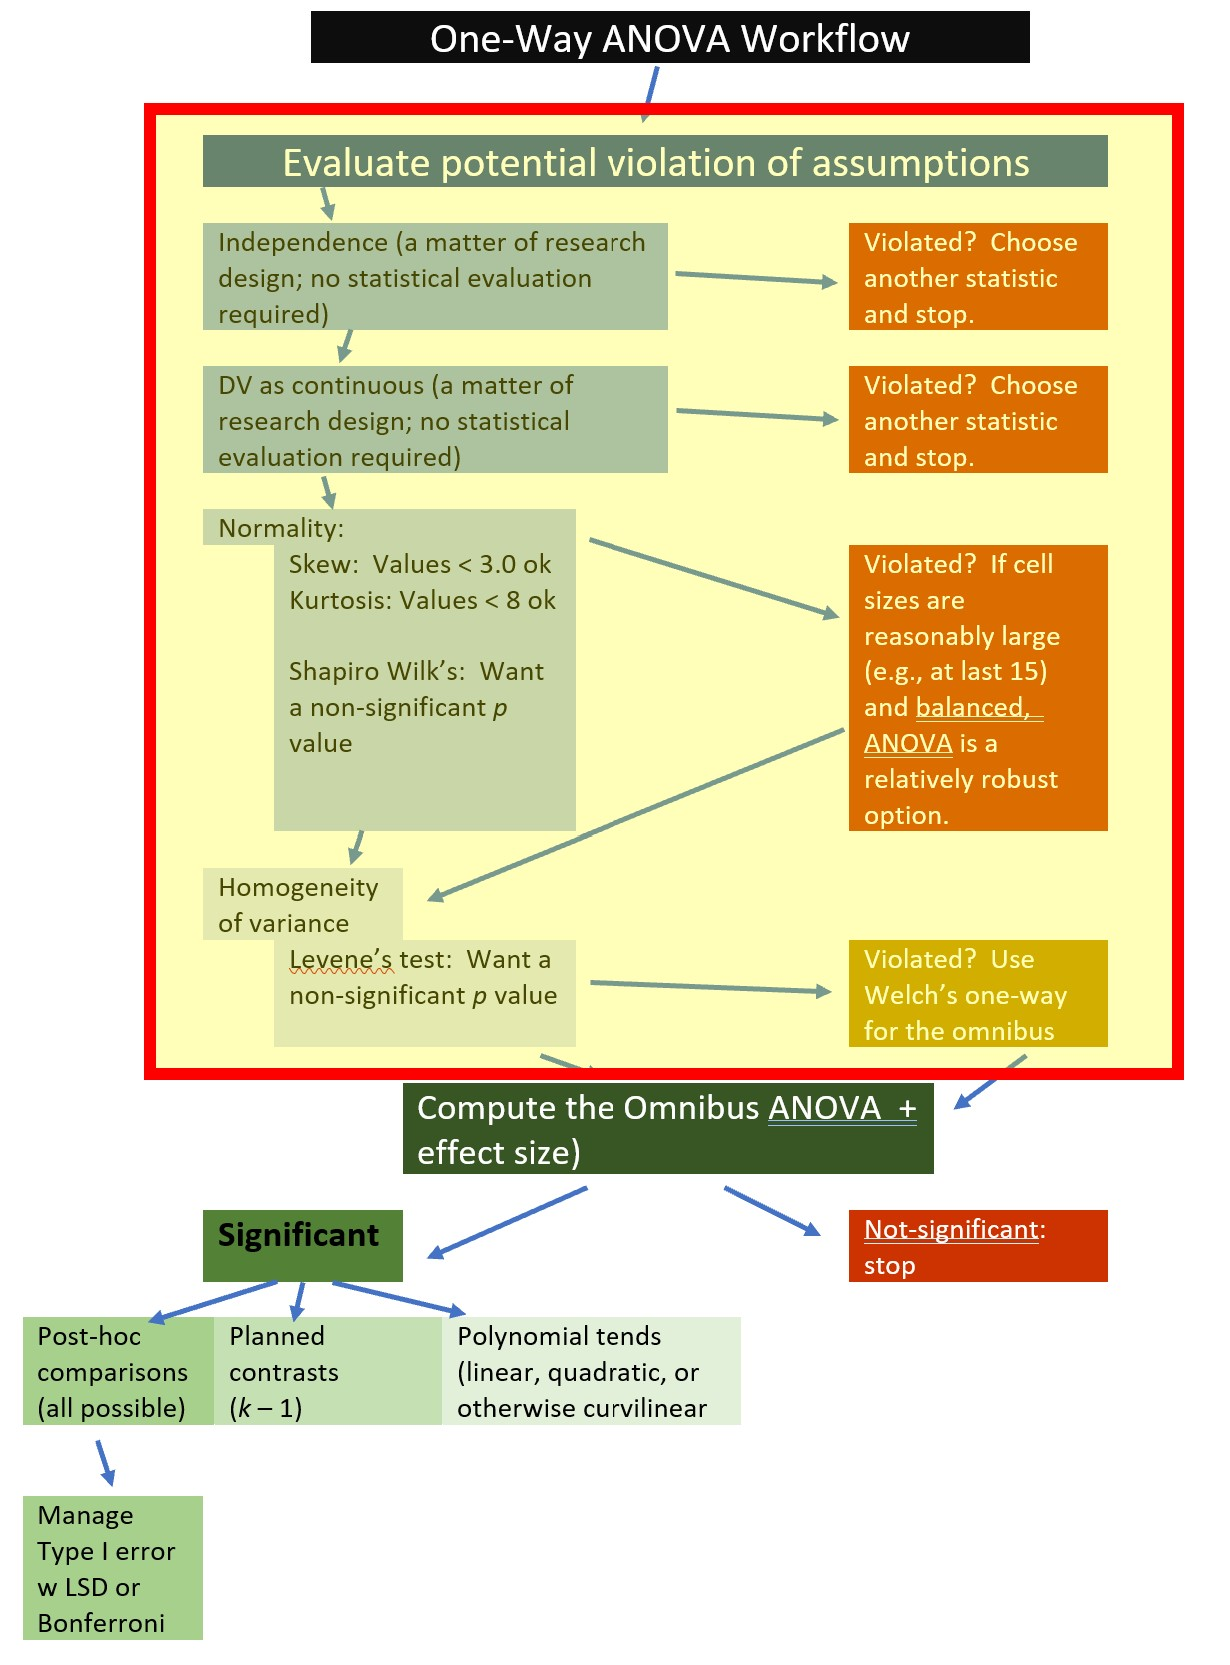
\includegraphics{images/oneway/OnewayWrkFlw_Asmptns.jpg}
\caption{An image of the workflow for one-way ANOVA, showing that we are at the beginning: evaluating the potential violation of the assumptions.}
\end{figure}

\hypertarget{evaluating-the-statistical-assumptions}{%
\subsection{Evaluating the Statistical Assumptions}\label{evaluating-the-statistical-assumptions}}

All statistical tests have some assumptions about the data. The one-way ANOVA has four assumptions:

\begin{itemize}
\tightlist
\item
  The dependent variable is normally distributed for each of the populations as defined by the different levels of the factor. We will examine this by

  \begin{itemize}
  \tightlist
  \item
    evaluating skew and kurtosis
  \item
    visually inspecting the distribution
  \item
    conduct a Shapiro Wilks test
  \item
    examine a QQ plot
  \end{itemize}
\item
  The variances of the dependent variable are the same for all populations. This is often termed the \emph{homogeneity of variance} assumption. We will examine this with

  \begin{itemize}
  \tightlist
  \item
    Levene's Test
  \end{itemize}
\item
  The cases represent \emph{random} samples from the populations and scores on the test variable are \emph{independent} of each other. That is, comparing related cases (e.g., parent/child, manager/employee, time1/time2) violates this assumption and this question would need to be evaluated by a different statistic such as repeated measures ANOVA or dyadic data analysis.

  \begin{itemize}
  \tightlist
  \item
    \emph{Independence} in observations is a research design issue. ANOVA is not robust to violating this assumption. When observations are correlated/dependent there is a dramatic increase in Type I error.
  \end{itemize}
\item
  The dependent variable is measured on an interval scale.

  \begin{itemize}
  \tightlist
  \item
    If the dependent variable is categorical, another statistic (such as logistic regression) should be chosen.
  \end{itemize}
\end{itemize}

\hypertarget{is-the-dependent-variable-normally-distributed-across-levels-of-the-factor}{%
\subsubsection{Is the dependent variable normally distributed across levels of the factor?}\label{is-the-dependent-variable-normally-distributed-across-levels-of-the-factor}}

From the \emph{psych} package, the \emph{describe()} function can be used to provide descriptive statistics (or, ``descriptives'') of continuously scaled variables (i.e., variables measured on the interval or ratio scale). In this simple example, we can specify the specific continuous, DV.

\begin{Shaded}
\begin{Highlighting}[]
\CommentTok{\#we name the function}
\CommentTok{\#in parentheses we list data source}
\NormalTok{psych}\SpecialCharTok{::}\FunctionTok{describe}\NormalTok{(accSIM30}\SpecialCharTok{$}\NormalTok{Accurate)}
\end{Highlighting}
\end{Shaded}

\begin{verbatim}
   vars  n mean   sd median trimmed  mad min max range  skew kurtosis   se
X1    1 90  1.6 0.67   1.73    1.62 0.68   0   3     3 -0.28    -0.48 0.07
\end{verbatim}

If we want descriptives for each level of the grouping variable (factor), we can use the \emph{describeBy()} function of the \emph{psych} package. The order of entry within the script is the DV followed by the grouping variable (IV).

\begin{Shaded}
\begin{Highlighting}[]
\CommentTok{\# It is unnecessary to create an object, but an object allows you to}
\CommentTok{\# do cool stuff, like write it to a .csv file and use that as a basis}
\CommentTok{\# for APA style tables In this script we can think \textquotesingle{}Accurate by COND\textquotesingle{}}
\CommentTok{\# meaning that the descriptives for accuracy will be grouped by COND}
\CommentTok{\# which is a categorical variable mat = TRUE presents the output in}
\CommentTok{\# matrix (table) form digits = 3 rounds the output to 3 decimal}
\CommentTok{\# places data = accSIM30 is a different (I think easier) way to}
\CommentTok{\# identify the object that holds the dataframe}
\NormalTok{des.mat }\OtherTok{\textless{}{-}}\NormalTok{ psych}\SpecialCharTok{::}\FunctionTok{describeBy}\NormalTok{(Accurate }\SpecialCharTok{\textasciitilde{}}\NormalTok{ COND, }\AttributeTok{mat =} \ConstantTok{TRUE}\NormalTok{, }\AttributeTok{digits =} \DecValTok{3}\NormalTok{, }\AttributeTok{data =}\NormalTok{ accSIM30)}
\CommentTok{\# Note. Recently my students and I have been having intermittent}
\CommentTok{\# struggles with the describeBy function in the psych package. We}
\CommentTok{\# have noticed that it is problematic when using .rds files and when}
\CommentTok{\# using data directly imported from Qualtrics. If you are having}
\CommentTok{\# similar difficulties, try uploading the .csv file and making the}
\CommentTok{\# appropriate formatting changes. displays the matrix object that we}
\CommentTok{\# just created}
\NormalTok{des.mat}
\end{Highlighting}
\end{Shaded}

\begin{verbatim}
    item  group1 vars  n  mean    sd median trimmed   mad   min   max range
X11    1 Control    1 30 1.756 0.460  1.893   1.767 0.392 0.781 2.745 1.964
X12    2     Low    1 30 1.900 0.630  2.007   1.918 0.458 0.655 3.000 2.345
X13    3    High    1 30 1.153 0.659  1.131   1.128 0.743 0.000 2.669 2.669
      skew kurtosis    se
X11 -0.275   -0.537 0.084
X12 -0.378   -0.465 0.115
X13  0.208   -0.690 0.120
\end{verbatim}

\begin{Shaded}
\begin{Highlighting}[]
\CommentTok{\# optional to write it to a .csv file}
\FunctionTok{write.csv}\NormalTok{(des.mat, }\AttributeTok{file =} \StringTok{"Table1.csv"}\NormalTok{)}
\end{Highlighting}
\end{Shaded}

Skew and kurtosis speaks to normal distributions. The skew and kurtosis indices in the \emph{psych} package are reported as \emph{z} scores. Regarding skew, values greater than 3.0 are generally considered ``severely skewed.'' Regarding kurtosis, ``severely kurtotic'' is argued to be anywhere greater 8 to 20 \citep{kline_principles_2016}.

The \emph{Shapiro-Wilks} test evaluates the hypothesis that the distribution of the data as a whole deviates from a comparable normal distribution. If the test is non-significant (\emph{p} \textgreater.05) the distribution of the sample is not significantly different from a normal distribution. If, however, the test is significant (\emph{p} \textless{} .05), then the sample distribution is significantly different from a normal distribution. The \emph{rstatix} package has a wrapper that can conduct the Shapiro-Wilks test for us.

\begin{Shaded}
\begin{Highlighting}[]
\NormalTok{shapiro }\OtherTok{\textless{}{-}}\NormalTok{ accSIM30 }\SpecialCharTok{\%\textgreater{}\%}
    \FunctionTok{group\_by}\NormalTok{(COND) }\SpecialCharTok{\%\textgreater{}\%}
\NormalTok{    rstatix}\SpecialCharTok{::}\FunctionTok{shapiro\_test}\NormalTok{(Accurate)}
\NormalTok{shapiro}
\end{Highlighting}
\end{Shaded}

\begin{verbatim}
# A tibble: 3 x 4
  COND    variable statistic     p
  <fct>   <chr>        <dbl> <dbl>
1 Control Accurate     0.954 0.215
2 Low     Accurate     0.944 0.115
3 High    Accurate     0.980 0.831
\end{verbatim}

The \(p\) values for the distributions of the dependent variable (accurate) in each of the three conditions are all well above .05. This tells us that the Accurate variable does not deviate from a statistically significant distribution (Control, \emph{W} = 0.954, \emph{p} = 0.215; Low, \emph{W} = 0.944, \emph{p} = 0.115; High, \emph{W} = 0.980, \emph{p} = 0.831).

There are limitations to the Shapiro-Wilks test. As the dataset being evaluated gets larger, the Shapiro-Wilks test becomes more sensitive to small deviations; this leads to a greater probability of rejecting the null hypothesis (null hypothesis being the values come from a normal distribution). Green and Salkind \citeyearpar{green_using_2014} advised that ANOVA is relatively robust to violations of normality if there are at least 15 cases per cell and the design is reasonably balanced (i.e., equal cell sizes).

\hypertarget{are-the-variances-of-the-dependent-variable-similar-across-the-levels-of-the-grouping-factor}{%
\subsubsection{Are the variances of the dependent variable similar across the levels of the grouping factor?}\label{are-the-variances-of-the-dependent-variable-similar-across-the-levels-of-the-grouping-factor}}

The Levene's test evaluates the ANOVA assumption that variances of the dependent variable for each level of the independent variable are similarly distributed. We want this to be non-significant (\(p\) \textgreater{} .05). If violated, we need to use an ANOVA test that is ``robust to the violation of the homogeneity of variance'' (e.g., Welch's oneway).

In R, Levene's test is found in the \emph{car} package.

\begin{Shaded}
\begin{Highlighting}[]
\CommentTok{\# Our set up is similar: Accurate by condition, followed by the}
\CommentTok{\# object that holds the dataframe, followed by the instruction to}
\CommentTok{\# center the analysis around the mean}
\NormalTok{levene }\OtherTok{\textless{}{-}}\NormalTok{ car}\SpecialCharTok{::}\FunctionTok{leveneTest}\NormalTok{(Accurate }\SpecialCharTok{\textasciitilde{}}\NormalTok{ COND, accSIM30, }\AttributeTok{center =}\NormalTok{ mean)}
\NormalTok{levene}
\end{Highlighting}
\end{Shaded}

\begin{verbatim}
Levene's Test for Homogeneity of Variance (center = mean)
      Df F value Pr(>F)
group  2  1.5315  0.222
      87               
\end{verbatim}

We write the result of the Levene's as \(F\)(2,87) = 1.532, \(p\) = 0.222. Because \(p\) \textgreater{} .05, we know that the result is nonsignficant -- that the variances of the three groups are not statistically significantly different than each other.

If the results had been statistically significantly different, we would have needed to use a Welch's \(F\) or robust version of ANOVA.

\hypertarget{summarizing-results-from-the-analysis-of-assumptions}{%
\subsubsection{Summarizing results from the analysis of assumptions}\label{summarizing-results-from-the-analysis-of-assumptions}}

It is common for an APA style results section to begin with a review of the evaluation of the statistical assumptions. As we have just finished these analyses, I will document what we have learned so far:

A one-way analysis of variance was conducted to evaluate the relationship between degree of racial loading of an exceptionalizing microaggression and the perceived accuracy of a research confederate's impression of the Asian or Asian American participant. The independent variable, condition, included three levels: control/none, low, and high levels of racial loading. Results of Levene's homogeneity of variance test indicated no violation of the homogeneity of variance assumption (\(F\){[}2,87{]} = 1.532, \(p\) = 0.222). Similarly, results of the Shapiro Wilk's test indicated no violation of the normality assumption in each of the cells (control, \emph{W} = 0.954, \emph{p} = 0.215; low, \emph{W} = 0.944, \emph{p} = 0.115; high, \emph{W} = 0.980, \emph{p} = 0.831).

Now we can move onto computing the omnibus ANOVA. \emph{Omnibus} is the term applied to the first \emph{F} test that evaluates if all groups have the same mean \citep{chen_relationship_2018}. If this test is not significant there is no evidence in the data to reject the null; that is, there is no evidence to suggest that group means are different. If it is significant -- and there are three or more groups -- follow-up testing will be needed to determine where the differences lie.

\hypertarget{computing-the-omnibus-anova}{%
\subsection{Computing the Omnibus ANOVA}\label{computing-the-omnibus-anova}}

Having met all the assumptions, we are now ready to calculate the omnibus \(F\) test.

\begin{figure}
\centering
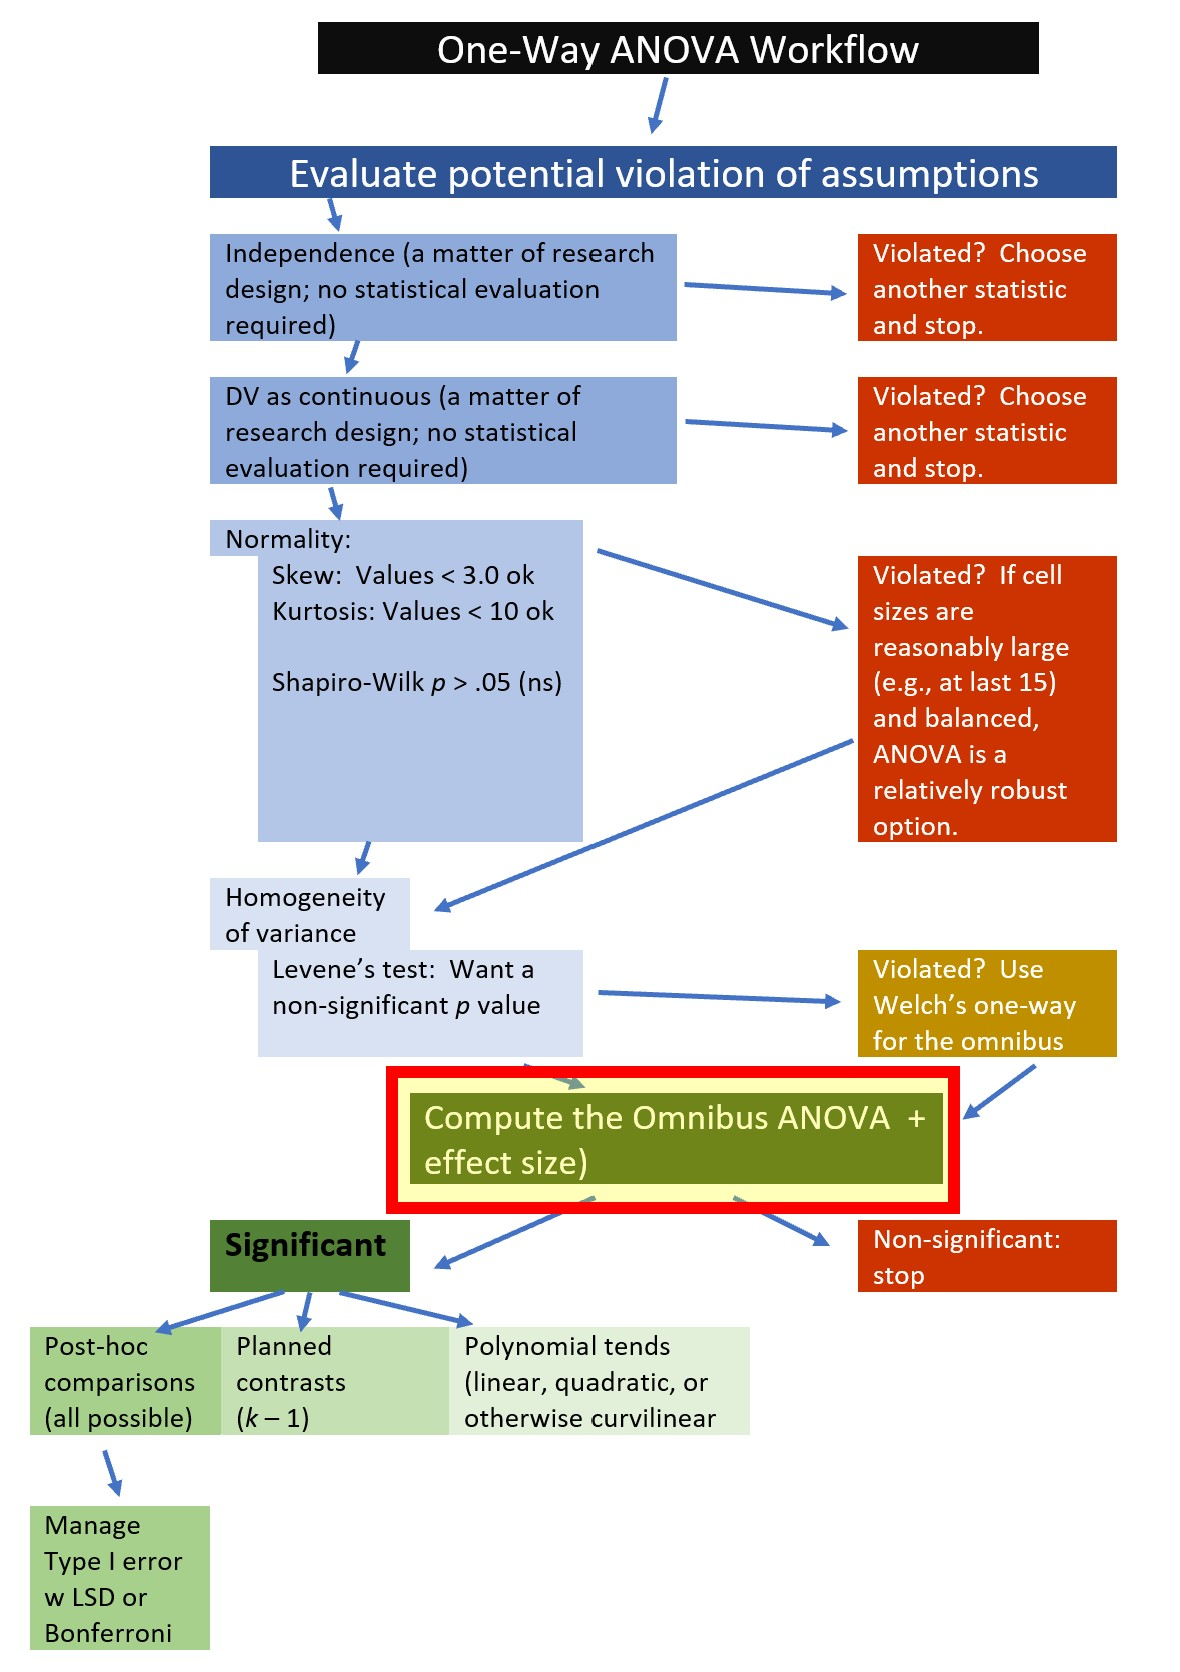
\includegraphics{images/oneway/OnewayWrkFlw_omnibus.jpg}
\caption{An image of the workflow for one-way ANOVA, showing that we are at the stage of computing the omnibus ANOVA.}
\end{figure}

ANOVA is a special case of the general linear model (regression is a ``not so special case'' of the general linear model), therefore we use the linear model function, \emph{aov()} to run the analysis.

In the code below, we predict Accuracy from COND (3 levels: control, low, high).

By assigning the results of the \emph{aov()} function to an object (omnibus) we can then use that object (think \emph{model}) in other functions to get details about our analysis.

\begin{Shaded}
\begin{Highlighting}[]
\CommentTok{\# the script looks familiar, \textquotesingle{}Accurate by Condition\textquotesingle{} DV \textasciitilde{} IV I say,}
\CommentTok{\# \textquotesingle{}DV by IV\textquotesingle{}}
\NormalTok{omnibus }\OtherTok{\textless{}{-}} \FunctionTok{aov}\NormalTok{(Accurate }\SpecialCharTok{\textasciitilde{}}\NormalTok{ COND, }\AttributeTok{data =}\NormalTok{ accSIM30)}
\CommentTok{\# prints the ANOVA output}
\FunctionTok{summary}\NormalTok{(omnibus)}
\end{Highlighting}
\end{Shaded}

\begin{verbatim}
            Df Sum Sq Mean Sq F value     Pr(>F)    
COND         2  9.432   4.716   13.57 0.00000745 ***
Residuals   87 30.246   0.348                       
---
Signif. codes:  0 '***' 0.001 '**' 0.01 '*' 0.05 '.' 0.1 ' ' 1
\end{verbatim}

Inserting the \emph{aov()} object (omnibus) into the summary command produces the ANOVA Source Table that we manually created above.

The values we see map onto those we calculated by hand. Our \(SS_M\) (9.432) plus \(SS_R\) (30.246) sum to equal the \(SS_T\) (39.678).

Dividing the two sums of squares by their respective degrees of freedom produces the means squared.

Then, dividing the \(MS_M\) (COND) by \(MS_R\) (4.716/0.348) provides the \emph{F} ratio. By using a table of \emph{F} critical values, we already knew that our \emph{F} value exceeded the value in the table of critical values. Here we see that \emph{p} = 0.000.

The ``\emph{F} string'' for an APA style results section should be written like this: \emph{F} (2, 87) = 13.566, \emph{p} \textless{} .001.

The object we created with the \emph{aov()} function is capable of producing much information. Applying the \emph{names()} function to the object can give us a list of values within it.

\begin{Shaded}
\begin{Highlighting}[]
\FunctionTok{names}\NormalTok{(omnibus)}
\end{Highlighting}
\end{Shaded}

\begin{verbatim}
 [1] "coefficients"  "residuals"     "effects"       "rank"         
 [5] "fitted.values" "assign"        "qr"            "df.residual"  
 [9] "contrasts"     "xlevels"       "call"          "terms"        
[13] "model"        
\end{verbatim}

One of the most commonly used functions to be applied to the \emph{aov()} objects is \emph{summary()}; but it's not the only one. Let's try some other options.

\begin{Shaded}
\begin{Highlighting}[]
\FunctionTok{model.tables}\NormalTok{ (omnibus, }\StringTok{"means"}\NormalTok{)}
\end{Highlighting}
\end{Shaded}

\begin{verbatim}
Tables of means
Grand mean
         
1.603042 

 COND 
COND
Control     Low    High 
 1.7562  1.9001  1.1528 
\end{verbatim}

The \emph{aov()} command has a quickplot feature.

\begin{Shaded}
\begin{Highlighting}[]
\FunctionTok{plot}\NormalTok{(omnibus) }
\end{Highlighting}
\end{Shaded}

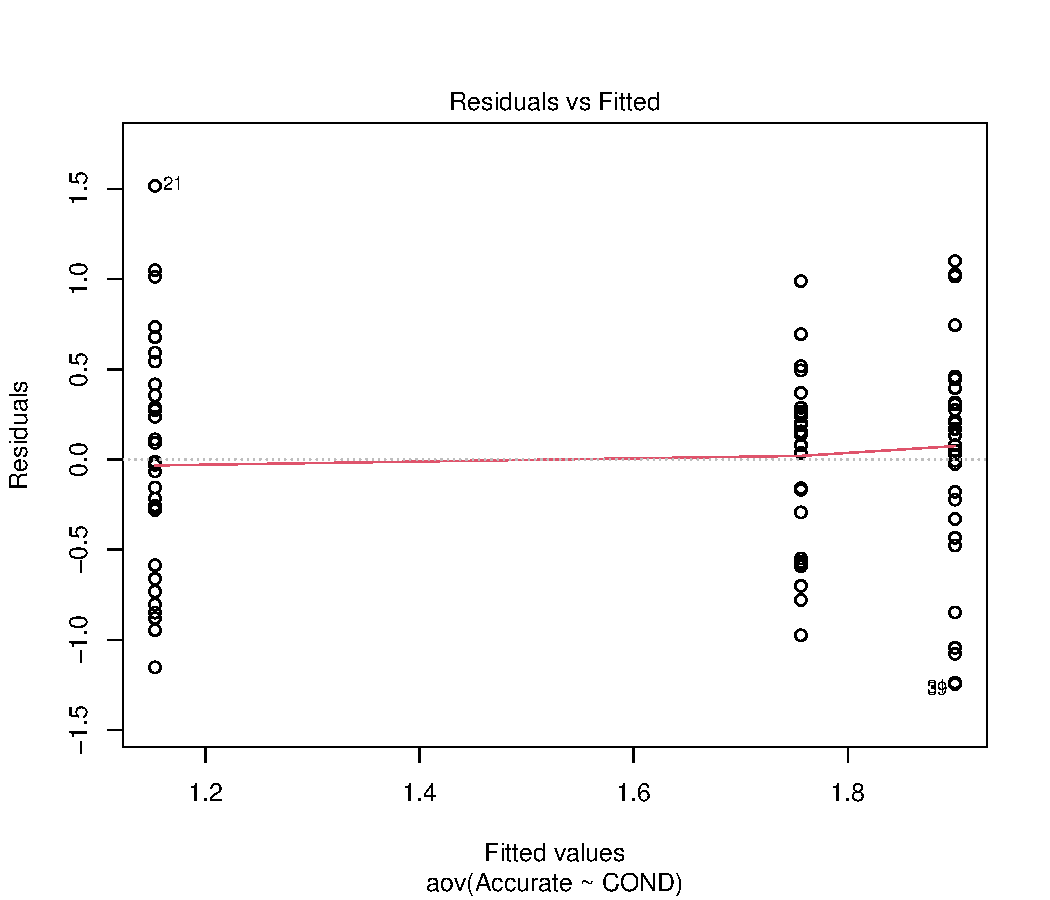
\includegraphics{ReCenterPsychStats_files/figure-latex/unnamed-chunk-84-1.pdf} 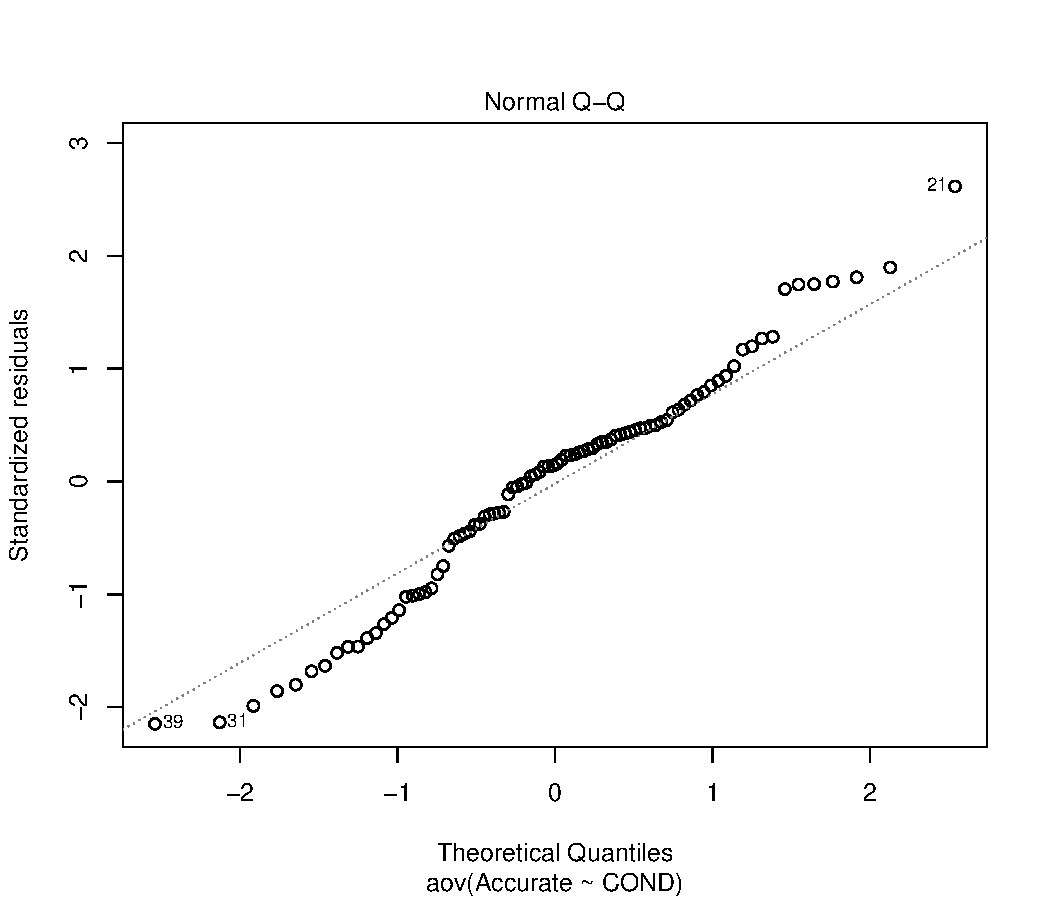
\includegraphics{ReCenterPsychStats_files/figure-latex/unnamed-chunk-84-2.pdf} 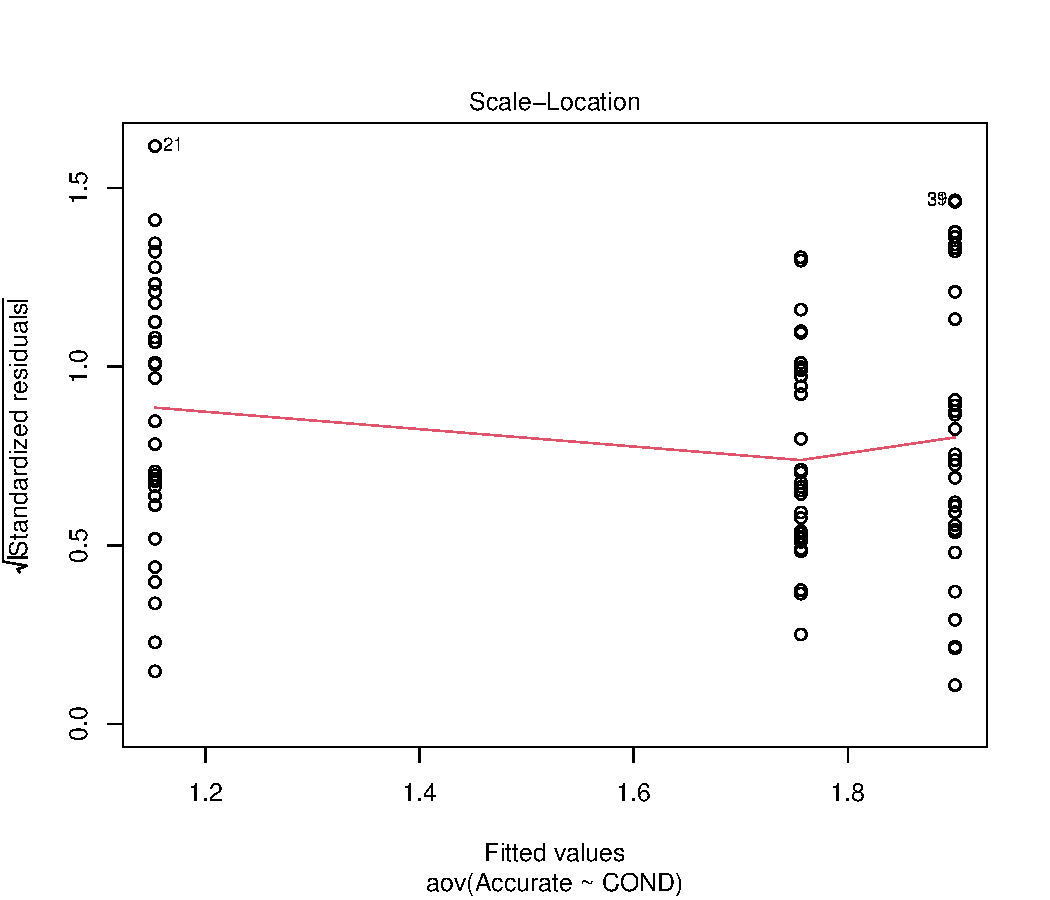
\includegraphics{ReCenterPsychStats_files/figure-latex/unnamed-chunk-84-3.pdf} 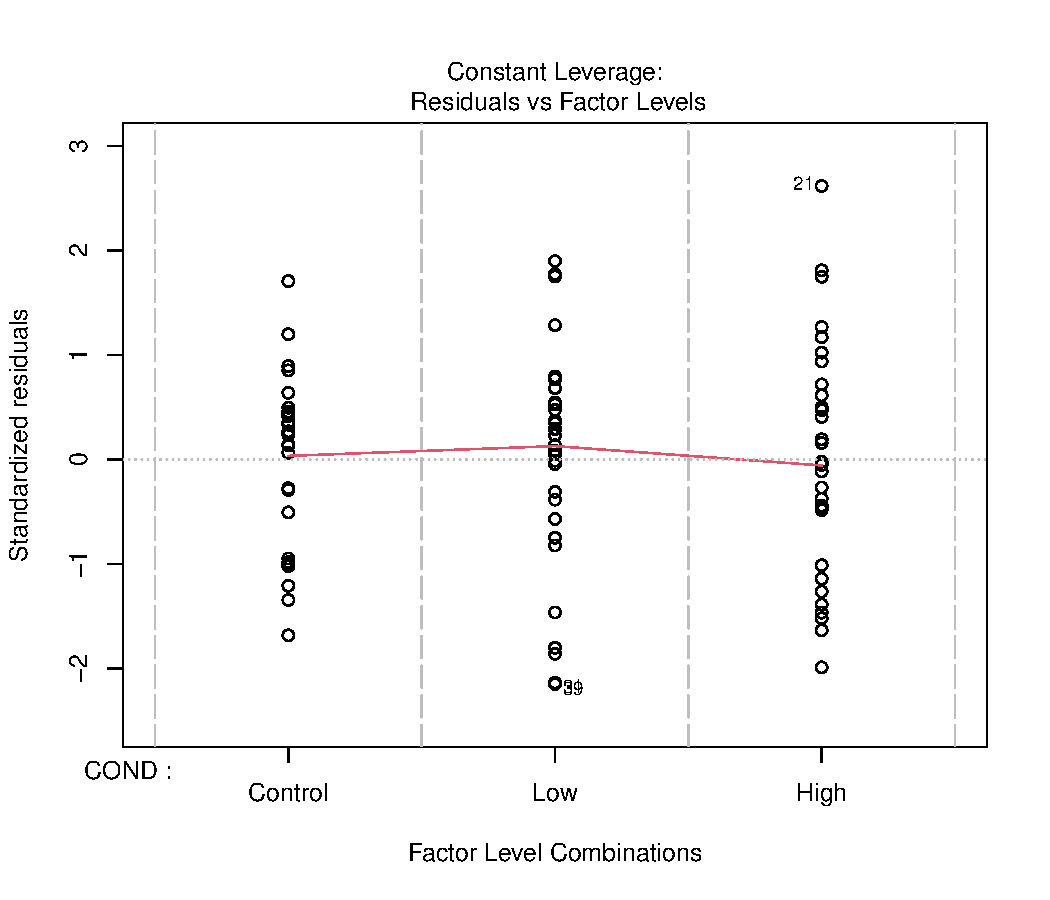
\includegraphics{ReCenterPsychStats_files/figure-latex/unnamed-chunk-84-4.pdf}

The first of the four plots fits the residuals. We already know from Levene's that we did not violate the homogeneity of variance test. With its straight line, this plot shows an equal spread across the three groups.

When the dots of the Q-Q plot map onto the diagonal, we have some indication of normality of the residuals (we want residuals to be normally distributed).

\hypertarget{effect-size-for-the-one-way-anova}{%
\subsubsection{Effect size for the one-way ANOVA}\label{effect-size-for-the-one-way-anova}}

\textbf{Eta squared} is one of the most commonly used measures of effect. It refers to the proportion of variability in the dependent variable/outcome that can be explained in terms of the independent variable/predictor. Traditional interpretive values are similar to the Pearson's \emph{r}:

\begin{itemize}
\tightlist
\item
  0.0 = no relationship
\item
  .02 = small
\item
  .13 = medium
\item
  .26 = large
\item
  1.0 = a perfect (one-to-one) correspondence
\end{itemize}

A useful summary of effect sizes, guide to interpreting their magnitudes, and common usage can be found \href{https://imaging.mrc-cbu.cam.ac.uk/statswiki/FAQ/effectSize}{here} \citep{watson_rules_2020}.

The formula for \(\eta^2\) is straightforward. If we think back to our hand-calculations of all the sums of squares, we can see that this is the proportion of variance that is accounted for by the model.

\[\eta ^{2}=\frac{SS_{M}}{SS_{T}}\]
Hand calculation, then, is straightforward.:

\begin{Shaded}
\begin{Highlighting}[]
\CommentTok{\#Calculated using the object names}
\NormalTok{SSMomnibus }\SpecialCharTok{/}\NormalTok{ (SSMomnibus }\SpecialCharTok{+}\NormalTok{ SSRomnibus)}
\end{Highlighting}
\end{Shaded}

\begin{verbatim}
[1] 0.238
\end{verbatim}

\begin{Shaded}
\begin{Highlighting}[]
\CommentTok{\#Re{-}calculated by using the numeric values}
\FloatTok{9.432}\SpecialCharTok{/}\NormalTok{(}\FloatTok{9.432} \SpecialCharTok{+} \FloatTok{30.246}\NormalTok{)}
\end{Highlighting}
\end{Shaded}

\begin{verbatim}
[1] 0.2377136
\end{verbatim}

\begin{Shaded}
\begin{Highlighting}[]
\CommentTok{\#Both options should produce the same result}
\end{Highlighting}
\end{Shaded}

The \emph{lsr} package includes an eta-squared calculator. To use it, we simply insert the model/object we created with the \emph{aov()} function to \emph{lsr}'s \emph{etaSquared()} function.

\begin{Shaded}
\begin{Highlighting}[]
\NormalTok{lsr}\SpecialCharTok{::}\FunctionTok{etaSquared}\NormalTok{(omnibus)}
\end{Highlighting}
\end{Shaded}

\begin{verbatim}
        eta.sq eta.sq.part
COND 0.2377226   0.2377226
\end{verbatim}

Notice that there are two effect sizes. We described eta-squared. Partial eta-squared is the default effect size reported in SPSS. There is a long history of debate about which to use. In certain circumstances (especially in more complicated analyses), partial-eta squared can be a bit more generous (i.e., larger than \(\eta^2\)). Thus, many prefer the reporting of the more cautious \(\eta^2\).

In our case, we see no difference between the two values. Differences begin to appear in datasets that are more complicated, such as when sample sizes across the levels of a factor differ.

\hypertarget{summarizing-results-from-the-omnibus-anova}{%
\subsubsection{Summarizing results from the omnibus ANOVA}\label{summarizing-results-from-the-omnibus-anova}}

Presenting the APA style results of the omnibus test is very straightforward:

Results indicated a significant effect of COND on accuracy perception \emph{F} (2, 87) = 13.566, \emph{p} \textless{} .001, \(\eta^2\) = 0.238.

\hypertarget{follow-up-to-the-omnibus-f}{%
\subsection{\texorpdfstring{Follow-up to the Omnibus \emph{F}}{Follow-up to the Omnibus F}}\label{follow-up-to-the-omnibus-f}}

The \emph{F}-test associated with the one-way ANOVA is the \emph{omnibus} -- giving the result for the overall test. Looking at the workflow for the one-way ANOVA we see that if we had had we had a non-significant \(F\), we would have stopped our analysis.

However, if the omnibus \(F\) is significant, we know that there is at least one pair of cells where there is a statistically significant difference. We have several ways (each with its own strengths/limitations) to figure out where these differences lie.

A very common option is to conduct post-hoc, pairwise comparisons.

\begin{figure}
\centering
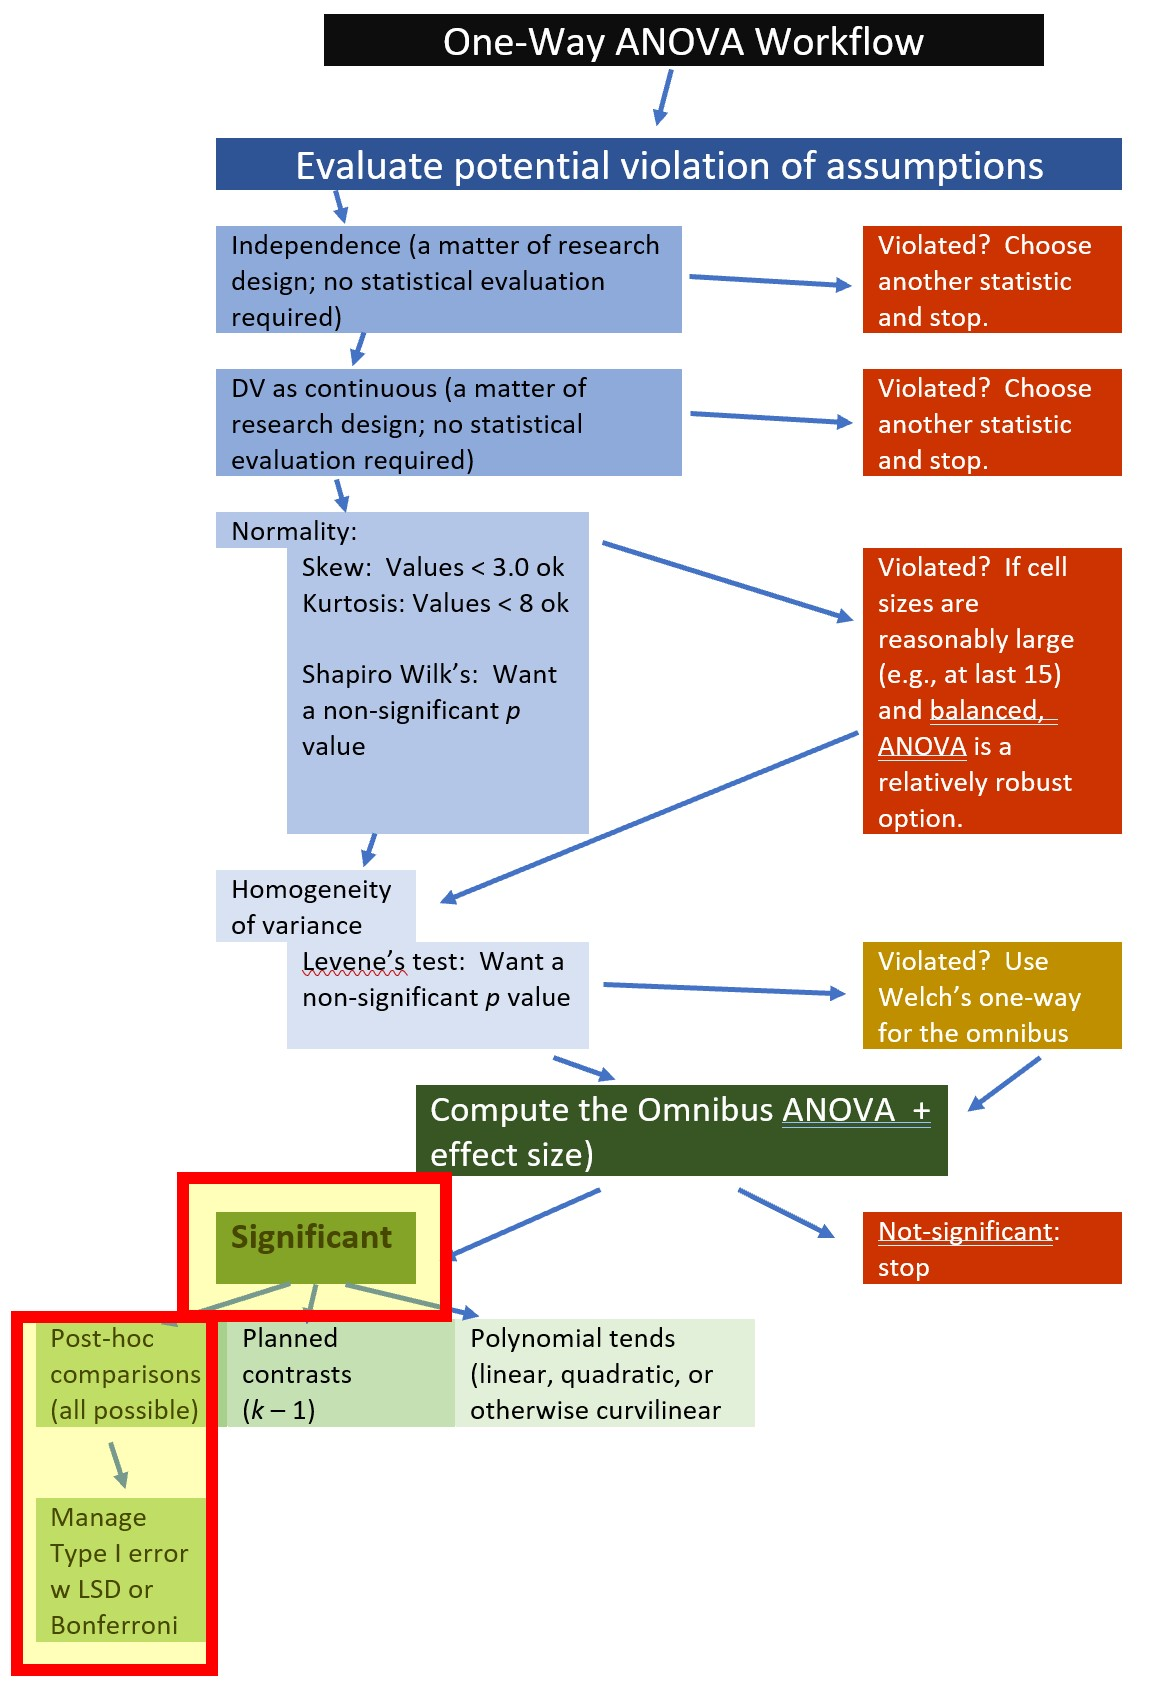
\includegraphics{images/oneway/OnewayWrkFlw_phoc.jpg}
\caption{An image of the workflow for one-way ANOVA, showing that we are at the stage of following a statistically significant omnibus F test and are now conducting posthoc comparisons.}
\end{figure}

\hypertarget{option-1-post-hoc-pairwise-comparisons}{%
\subsubsection{OPTION 1: Post-hoc, pairwise, comparisons}\label{option-1-post-hoc-pairwise-comparisons}}

Post-hoc, pairwise comparisons are:

\begin{itemize}
\tightlist
\item
  used for exploratory work when no firm hypotheses were articulated a priori,
\item
  used to compare the means of all combinations of pairs of an experimental condition,
\item
  less powerful than planned comparisons b/c strict criterion for significance must be used.
\end{itemize}

Helpful information about how to conduct post-hoc pairwise comparisons in R can be found at the \href{https://stats.idre.ucla.edu/r/faq/how-can-i-do-post-hoc-pairwise-comparisons-in-r/}{UCLA Institute for Digital Research and Education site} \citep{noauthor_how_nodate}.

\begin{Shaded}
\begin{Highlighting}[]
\FunctionTok{pairwise.t.test}\NormalTok{(accSIM30}\SpecialCharTok{$}\NormalTok{Accurate, accSIM30}\SpecialCharTok{$}\NormalTok{COND, }\AttributeTok{p.adj =} \StringTok{"none"}\NormalTok{)}
\end{Highlighting}
\end{Shaded}

\begin{verbatim}
    Pairwise comparisons using t tests with pooled SD 

data:  accSIM30$Accurate and accSIM30$COND 

     Control Low      
Low  0.34709 -        
High 0.00015 0.0000042

P value adjustment method: none 
\end{verbatim}

\begin{Shaded}
\begin{Highlighting}[]
\CommentTok{\#can swap "bonf" or "holm" for p.adj}
\end{Highlighting}
\end{Shaded}

The output only provides the \(p\) values associated with the mean differences in each of the conditions. We see that \(p < .05\) when high is compared to control (0.00015) and high is compared to low (0.0000042). An APA style reporting results of these typically involves referencing the means (often reported in a table of means and standard deviations) or mean differences (hand calculated) with their \emph{p} values.

\textbf{Should we be concerned about Type I error?}

Recall that \emph{Type I error} is the concern about false positives -- that we would incorrectly reject a true null hypothesis (that we would say that there is a statistically significant difference when there is not one). This concern increases when we have a large number of pairwise comparisons.

Green and Salkind \citeyearpar{green_using_2014} reviewed three options for managing Type I error.

\begin{itemize}
\tightlist
\item
  Traditional Bonferroni:

  \begin{itemize}
  \tightlist
  \item
    Adjusts the \emph{p} value upward by multiplying it (the raw \emph{p} values) by the number of comparisons being completed. This holds the \emph{total} Type I error rate across these tests to \(\alpha\) (usually .05). The traditional Bonferroni is simple and therefore attractive, but when \emph{p} values hover around .05, it can be too restrictive.
  \end{itemize}
\item
  Holms Sequential Bonferroni:

  \begin{itemize}
  \tightlist
  \item
    We'll describe this in more detail later. Briefly, it allows us to rank order the comparisons by their \emph{p} value (smallest to largest). We determine the significance of each \emph{p} value \emph{sequentially} where the criteria for significance is incrementally relaxed.
  \end{itemize}
\item
  LSD method:

  \begin{itemize}
  \tightlist
  \item
    Permitted when there are only three pairwise comparisons among three groups, researchers can leave the \emph{p} values as they are. Since the Tran and Lee \citeyearpar{tran_you_2014} research vignette is one of those circumstances, I will not make adjustments for Type I error. That is, I would claim the LSD and cite Green and Salkind \citeyearpar{green_using_2014} as justification for that decision.
  \end{itemize}
\end{itemize}

There is, though, an even more powerful approach\ldots{}

\hypertarget{option-2-planned-contrasts-non-orthogonal}{%
\subsubsection{OPTION 2: Planned contrasts (non-orthogonal)}\label{option-2-planned-contrasts-non-orthogonal}}

Another option is to evaluate planned comparisons.

\begin{figure}
\centering
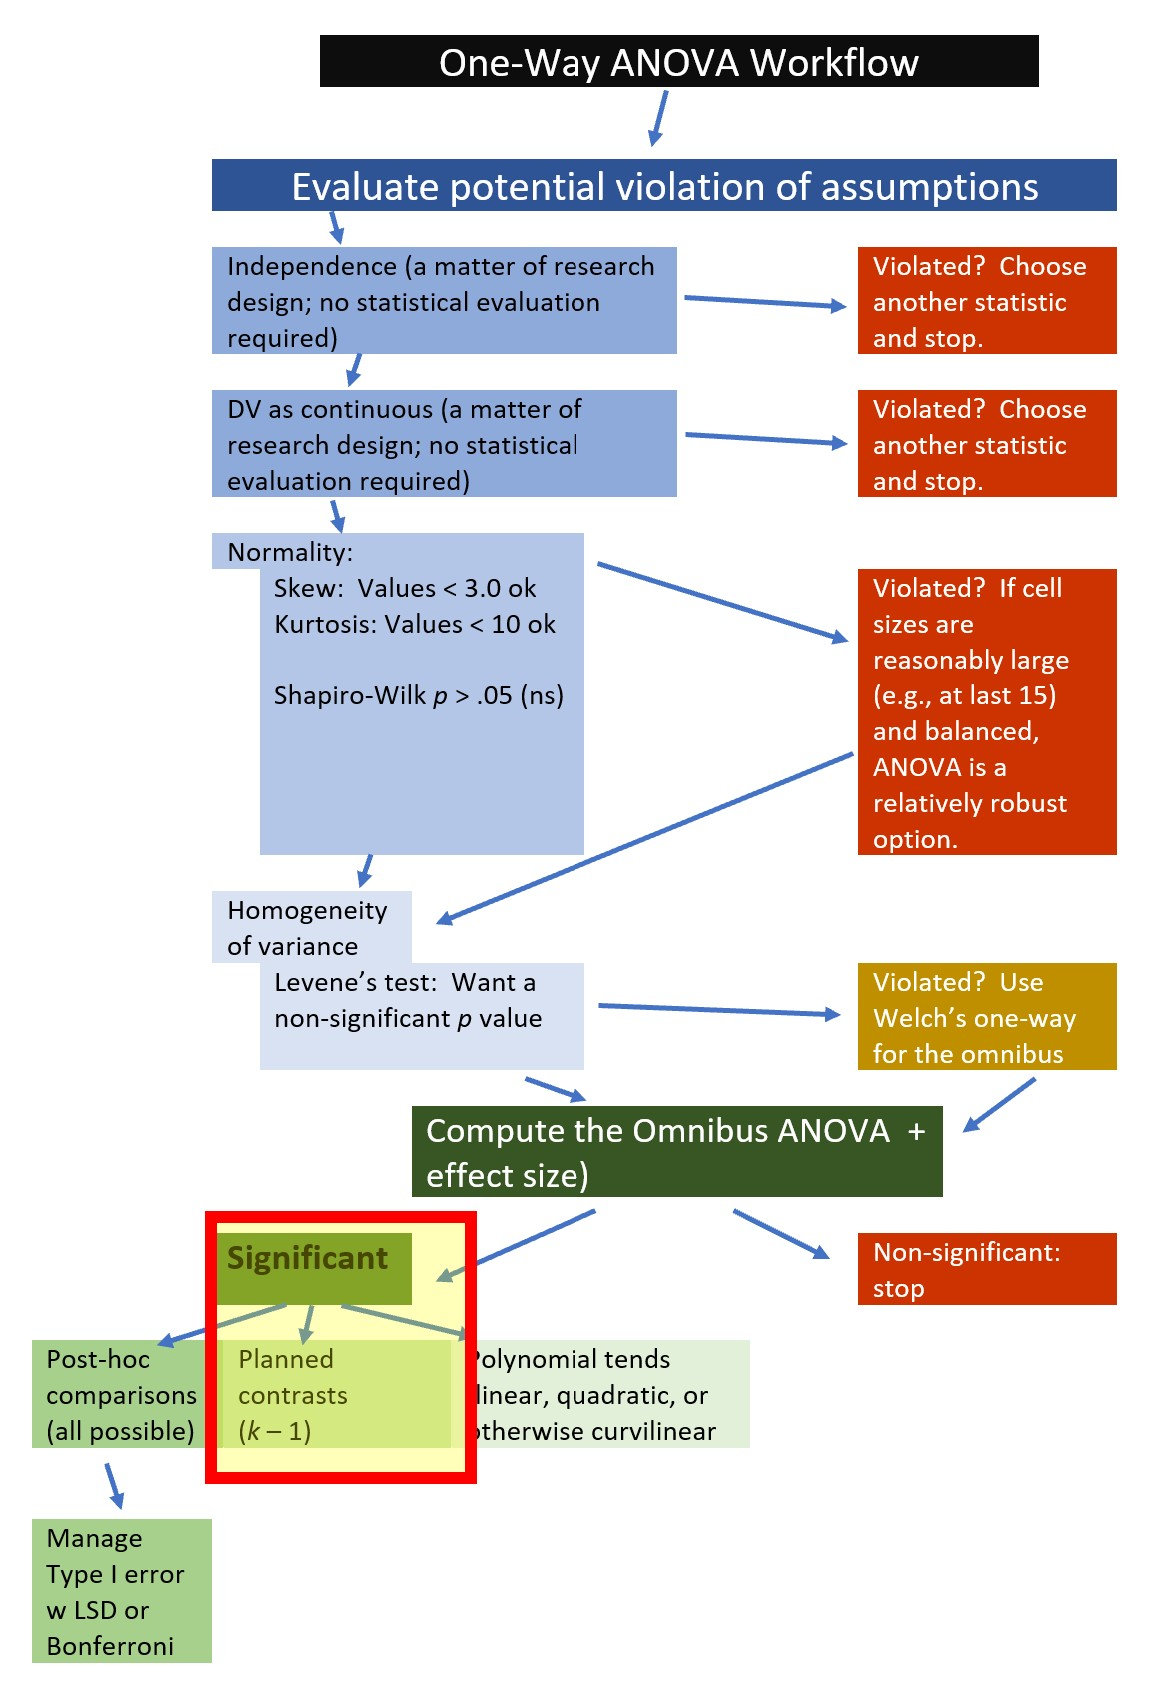
\includegraphics{images/oneway/OnewayWrkFlw_planned.jpg}
\caption{An image of the workflow for one-way ANOVA, showing that we are at the following up to a significant omnibus F by conducting planned comparisons}
\end{figure}

Planned comparisons are

\begin{itemize}
\tightlist
\item
  theory-driven comparisons constructed prior to data collection,
\item
  based on the idea of partitioning the variance created by the overall effect of group differences into gradually smaller portions of variance, and
\item
  more powerful than post-hoc tests.
\end{itemize}

Planned contrasts involve further considerations regarding the \emph{partitioning of variance.}

\begin{itemize}
\tightlist
\item
  There will always be \emph{k}-1 contrasts.
\item
  Each contrast must involve only two chunks of variance.
\end{itemize}

\emph{Orthogonal} contrasts are even more sophisticated. Essential to conducting an orthogonal contrast is the requirement that if a group is singled out in one comparison it should be excluded from subsequent contrasts. The typical, orthogonal scenario with three ordered groups has only two contrasts:

\begin{enumerate}
\def\labelenumi{\arabic{enumi}.}
\tightlist
\item
  Control versus low and high (because control was excluded, it should not reappear in the next contrast)
\item
  Low versus high
\end{enumerate}

Underlying the \emph{aov()} program is the linear model (``lm''). We could have used it to calculate the omnibus ANOVA, but it has clunky output.

We use it now to retrieve some contrast information. The code below is a planned comparison that uses the coding in the database (created when we formatted COND as an ordered factor) to compare the lowest coded group (control was 1, low was 2, high was 3) to the other two groups.

\begin{Shaded}
\begin{Highlighting}[]
\FunctionTok{summary.lm}\NormalTok{(omnibus)}
\end{Highlighting}
\end{Shaded}

\begin{verbatim}
Call:
aov(formula = Accurate ~ COND, data = accSIM30)

Residuals:
     Min       1Q   Median       3Q      Max 
-1.24533 -0.32092  0.08642  0.30101  1.51646 

Coefficients:
            Estimate Std. Error t value             Pr(>|t|)    
(Intercept)   1.7562     0.1076  16.314 < 0.0000000000000002 ***
CONDLow       0.1439     0.1522   0.945             0.347095    
CONDHigh     -0.6034     0.1522  -3.963             0.000151 ***
---
Signif. codes:  0 '***' 0.001 '**' 0.01 '*' 0.05 '.' 0.1 ' ' 1

Residual standard error: 0.5896 on 87 degrees of freedom
Multiple R-squared:  0.2377,    Adjusted R-squared:  0.2202 
F-statistic: 13.57 on 2 and 87 DF,  p-value: 0.000007446
\end{verbatim}

From the above, regression output, we see that there was not a statistically significant difference between CONDControl and CONDLow (\emph{p} = 0.347). There were statistically significant difference when CONDControl (the intercept) was compared to CONDHigh (\emph{p} \textless{} .001).

Note that these tests are conducted as \emph{t} tests. Why? We are comparing only two groups and can use the \emph{t} distribution.

Also note that these involved the comparison of the control group to low; then the control to high. This is consistent with an orthogonal contrast in that there are \emph{k} - 1 contrasts (two contrasts with three original groups). However it is inconsistent with the requriement that once a group is singled out, it should not be used in a subsequent contrast. Therefore, it is quite possible we want something different.

\hypertarget{option-3-planned-contrasts-orthogonal}{%
\subsubsection{OPTION 3: Planned contrasts (orthogonal)}\label{option-3-planned-contrasts-orthogonal}}

\textbf{Step 1: } Specify our contrasts

\begin{itemize}
\tightlist
\item
  Specifying the contrasts means you know their order within the factor
\item
  Early in the data preparation, we created an ordered factor with Control, Low, High as the order.
\item
  We want orthogonal contrasts, this means there will be

  \begin{itemize}
  \tightlist
  \item
    \emph{k} - 1 contrasts; with three groups we will have two contrasts
  \item
    once we single out a condition for comparison, we cannot use it again.
  \end{itemize}
\end{itemize}

In \emph{contrast1} we compare the control condition to the combined low and high conditions.
In \emph{contrast2} we discard the control condition (it was already singled out) and we compare the low and high conditions.

This is sensible because we likely hypothesize that any degree of racially loaded stereotypes may have a deleterious outcome, so we first compare control to the two conditions with any degree of racial loading. Subsequently, we compare the low and high levels of the factor.

\textbf{Step 2:} Bind them together and check the output to ensure that we've mapped them correctly.

\begin{Shaded}
\begin{Highlighting}[]
\CommentTok{\# Contrast1 compares Control against the combined effects of Low and}
\CommentTok{\# High.}
\NormalTok{contrast1 }\OtherTok{\textless{}{-}} \FunctionTok{c}\NormalTok{(}\SpecialCharTok{{-}}\DecValTok{2}\NormalTok{, }\DecValTok{1}\NormalTok{, }\DecValTok{1}\NormalTok{)}

\CommentTok{\# Contrast2 excludes Control; compares Low to High.}
\NormalTok{contrast2 }\OtherTok{\textless{}{-}} \FunctionTok{c}\NormalTok{(}\DecValTok{0}\NormalTok{, }\SpecialCharTok{{-}}\DecValTok{1}\NormalTok{, }\DecValTok{1}\NormalTok{)}

\CommentTok{\# binding the contrasts together}
\FunctionTok{contrasts}\NormalTok{(accSIM30}\SpecialCharTok{$}\NormalTok{COND) }\OtherTok{\textless{}{-}} \FunctionTok{cbind}\NormalTok{(contrast1, contrast2)}
\NormalTok{accSIM30}\SpecialCharTok{$}\NormalTok{COND}
\end{Highlighting}
\end{Shaded}

\begin{verbatim}
 [1] High    High    High    High    High    High    High    High    High   
[10] High    High    High    High    High    High    High    High    High   
[19] High    High    High    High    High    High    High    High    High   
[28] High    High    High    Low     Low     Low     Low     Low     Low    
[37] Low     Low     Low     Low     Low     Low     Low     Low     Low    
[46] Low     Low     Low     Low     Low     Low     Low     Low     Low    
[55] Low     Low     Low     Low     Low     Low     Control Control Control
[64] Control Control Control Control Control Control Control Control Control
[73] Control Control Control Control Control Control Control Control Control
[82] Control Control Control Control Control Control Control Control Control
attr(,"contrasts")
        contrast1 contrast2
Control        -2         0
Low             1        -1
High            1         1
Levels: Control Low High
\end{verbatim}

Thinking back to the hand-calculations and contrast mapping, the table of weights that R just produced confirms that

\begin{itemize}
\tightlist
\item
  Contrast 1 compares the control condition against the levels with any racial loading.
\item
  Contrast 2 compares the low and high loadings.
\end{itemize}

\textbf{Step 3:} Create a new \emph{aov()} model

\begin{Shaded}
\begin{Highlighting}[]
\CommentTok{\# create a new object, the ANOVA looks the same, but it will now}
\CommentTok{\# consider the contrasts (this is where order{-}of{-}operations matters)}
\NormalTok{accPlanned }\OtherTok{\textless{}{-}} \FunctionTok{aov}\NormalTok{(Accurate }\SpecialCharTok{\textasciitilde{}}\NormalTok{ COND, }\AttributeTok{data =}\NormalTok{ accSIM30)}
\FunctionTok{summary.lm}\NormalTok{(accPlanned)}
\end{Highlighting}
\end{Shaded}

\begin{verbatim}
Call:
aov(formula = Accurate ~ COND, data = accSIM30)

Residuals:
     Min       1Q   Median       3Q      Max 
-1.24533 -0.32092  0.08642  0.30101  1.51646 

Coefficients:
              Estimate Std. Error t value             Pr(>|t|)    
(Intercept)    1.60304    0.06215  25.793 < 0.0000000000000002 ***
CONDcontrast1 -0.07658    0.04395  -1.742                0.085 .  
CONDcontrast2 -0.37365    0.07612  -4.909           0.00000425 ***
---
Signif. codes:  0 '***' 0.001 '**' 0.01 '*' 0.05 '.' 0.1 ' ' 1

Residual standard error: 0.5896 on 87 degrees of freedom
Multiple R-squared:  0.2377,    Adjusted R-squared:  0.2202 
F-statistic: 13.57 on 2 and 87 DF,  p-value: 0.000007446
\end{verbatim}

\begin{Shaded}
\begin{Highlighting}[]
\FunctionTok{contrasts}\NormalTok{(accSIM30}\SpecialCharTok{$}\NormalTok{COND) }\OtherTok{\textless{}{-}} \FunctionTok{cbind}\NormalTok{(}\FunctionTok{c}\NormalTok{(}\SpecialCharTok{{-}}\DecValTok{2}\NormalTok{, }\DecValTok{1}\NormalTok{, }\DecValTok{1}\NormalTok{), }\FunctionTok{c}\NormalTok{(}\DecValTok{0}\NormalTok{, }\SpecialCharTok{{-}}\DecValTok{1}\NormalTok{, }\DecValTok{1}\NormalTok{))}
\end{Highlighting}
\end{Shaded}

These planned contrasts show that when the control condition is compared to the combined low and high racial loading conditions, there is not a statistically significant difference, \emph{t}(87) = -1.742, \emph{p} = 0.085. However, when the low and high racial loading conditions are compared, there is a statistically significant difference, \emph{t}(87) = -4.909, \emph{p} \textless{} 0.001.

\hypertarget{option-4-trend-polynomial-analysis}{%
\subsubsection{OPTION 4: Trend (polynomial) analysis}\label{option-4-trend-polynomial-analysis}}

\begin{figure}
\centering
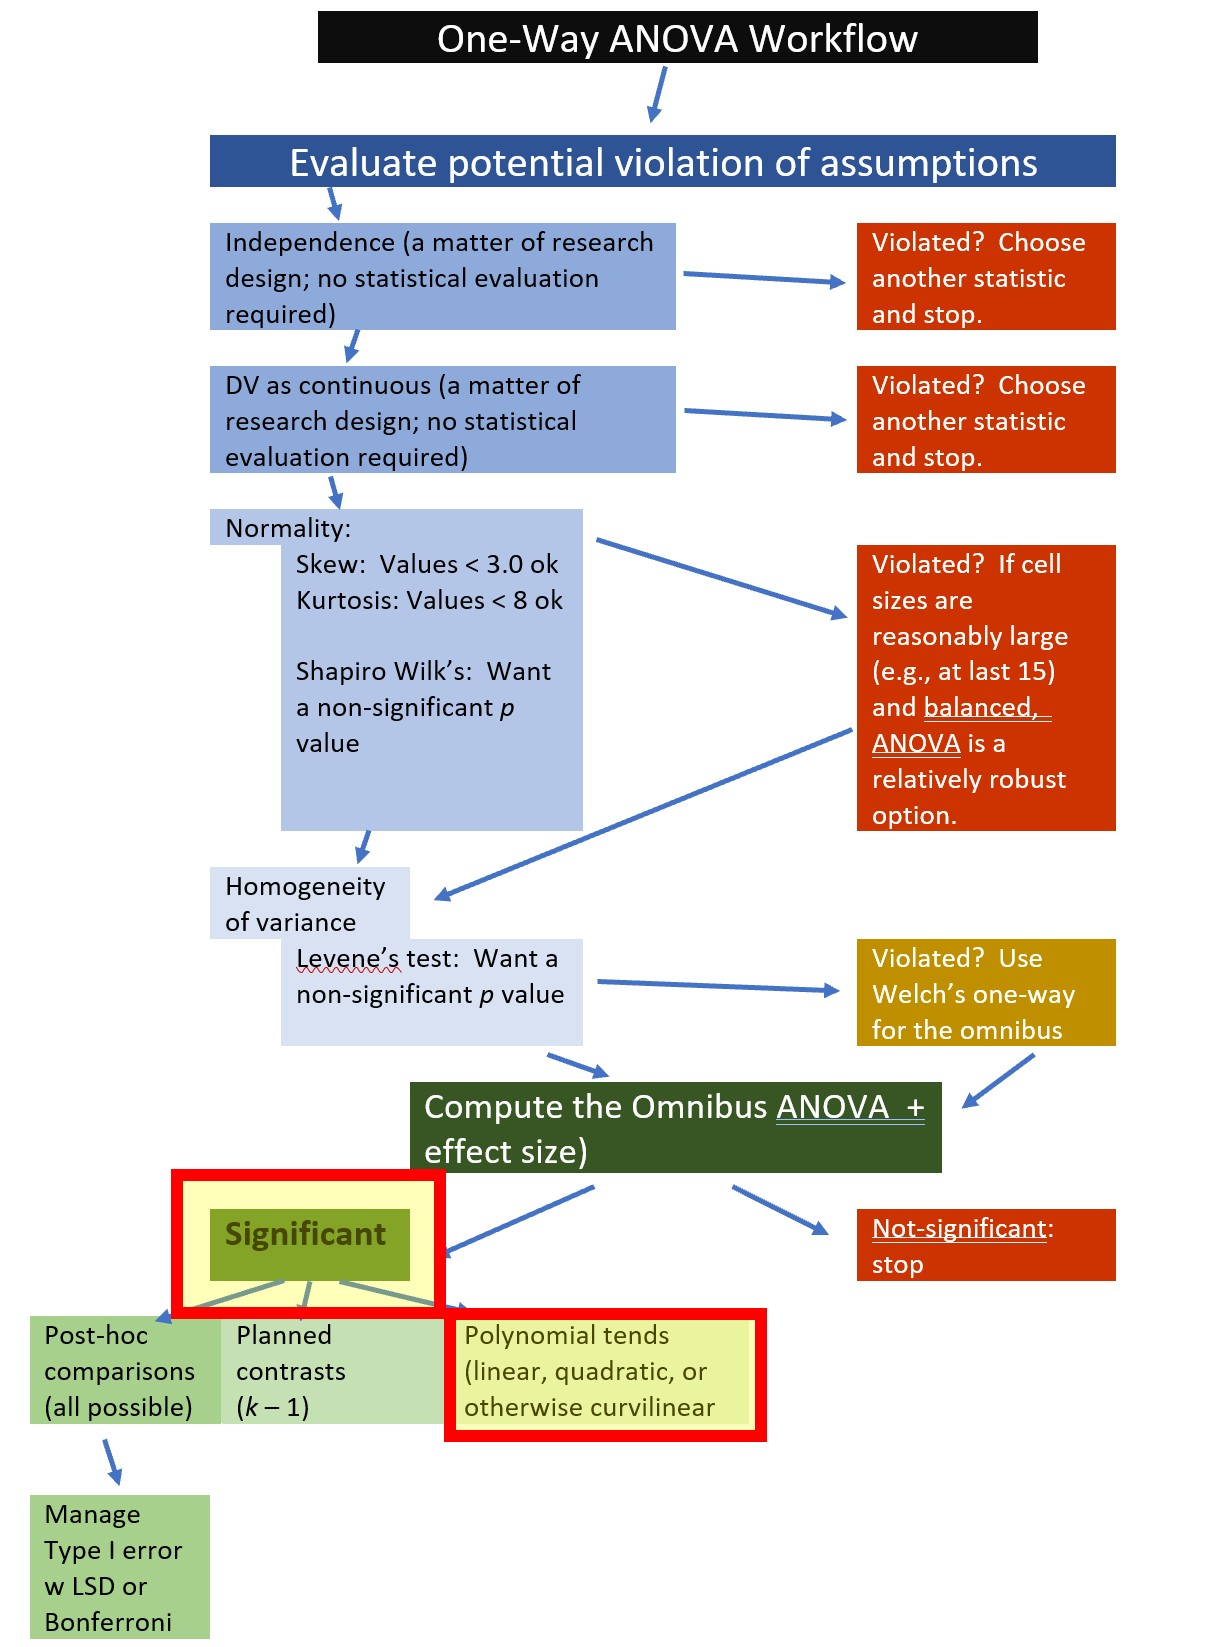
\includegraphics{images/oneway/OnewayWrkFlw_poly.jpg}
\caption{An image of the workflow for one-way ANOVA, showing that we are at the following up to a significant omnibus F by assessing for a polynomial trend}
\end{figure}

Polynomial contrasts evaluate for the presence of a linear (or curvilinear) pattern in the data. To detect a trend, the data must be coded in an ascending order and it needs to be a sensible, theoretically defensible, comparison. Our data has a theoretically ordered effect (control, low racially loaded condition, high racially loaded condition). Recall that we created an ordered factor when we imported the data.

In a polynomial analysis, the statistical analysis looks across the ordered means to see if they fit a linear or curvilinear shape that is one less than the number of levels. Our factor has three levels, therefore the polynomial contrast can check for a linear shape (.L) or a quadratic (one change in direction) shape (.Q). If we had four levels, the contr.poly could check for cubic change (two changes in direction). Conventionally, when more than one trend is significant, we intepret the most complex one (i.e., quadratic over linear).

\begin{Shaded}
\begin{Highlighting}[]
\FunctionTok{contrasts}\NormalTok{(accSIM30}\SpecialCharTok{$}\NormalTok{COND) }\OtherTok{\textless{}{-}} \FunctionTok{contr.poly}\NormalTok{(}\DecValTok{3}\NormalTok{)}
\NormalTok{accTrend }\OtherTok{\textless{}{-}} \FunctionTok{aov}\NormalTok{(Accurate }\SpecialCharTok{\textasciitilde{}}\NormalTok{ COND, }\AttributeTok{data =}\NormalTok{ accSIM30)}
\FunctionTok{summary.lm}\NormalTok{(accTrend)}
\end{Highlighting}
\end{Shaded}

\begin{verbatim}
Call:
aov(formula = Accurate ~ COND, data = accSIM30)

Residuals:
     Min       1Q   Median       3Q      Max 
-1.24533 -0.32092  0.08642  0.30101  1.51646 

Coefficients:
            Estimate Std. Error t value             Pr(>|t|)    
(Intercept)  1.60304    0.06215  25.793 < 0.0000000000000002 ***
COND.L      -0.42665    0.10765  -3.963             0.000151 ***
COND.Q      -0.36384    0.10765  -3.380             0.001087 ** 
---
Signif. codes:  0 '***' 0.001 '**' 0.01 '*' 0.05 '.' 0.1 ' ' 1

Residual standard error: 0.5896 on 87 degrees of freedom
Multiple R-squared:  0.2377,    Adjusted R-squared:  0.2202 
F-statistic: 13.57 on 2 and 87 DF,  p-value: 0.000007446
\end{verbatim}

A quick peek back at an early plot shows illustrates the quadratic trend that was supported by the analysis.

Results of our polynomial contrast suggested statistically significant results for both linear \(t(87) = -3.963 , p < .001\) and quadratic \(t(87) = -3.380, p = .001\) trends.

\hypertarget{which-set-of-follow-up-tests-do-we-report}{%
\subsubsection{Which set of follow-up tests do we report?}\label{which-set-of-follow-up-tests-do-we-report}}

It depends! What best tells the story of your data? Here are some things to consider.

\begin{itemize}
\tightlist
\item
  If the post-hoc comparisons are robustly statistically significant (and controlling Type I error is not going to change that significance), I think this provides good information and I would lean toward reporting those.
\item
  If \emph{p} values are hovering around 0.05, an orthogonal contrast will offer more power because

  \begin{itemize}
  \tightlist
  \item
    a \emph{k} - 1 comparison will be more powerful
  \item
    a priori theory is compelling
  \end{itemize}
\item
  The polynomial can be a useful descriptive addition if there is a linear or quadratic relationship that is sensible or interesting.
\end{itemize}

Although I would report either the post-hoc or planned contrasts, I will sometimes add a polynomial if it clarifies the result (i.e., there is a meaningful linear or curvilinear pattern essential to understanding the data).

\hypertarget{what-if-we-violated-the-homogeneity-of-variance-test}{%
\subsection{What if we Violated the Homogeneity of Variance test?}\label{what-if-we-violated-the-homogeneity-of-variance-test}}

The \emph{oneway.test} produces Welch's \emph{F} -- a test more robust to violation of the homogeneity of variance assumption. The Welch's approach to attenuating error or erroneous conclusions caused by violations of the homogeneity of variance assumption is to adjust the residual degrees of freedom used to produce the Welch's \emph{F}-ratio.

Another common correction is the Brown and Forsythe \emph{F}-ratio. At this time I have not located and tried an R package that produces this.

\begin{Shaded}
\begin{Highlighting}[]
\FunctionTok{oneway.test}\NormalTok{(Accurate }\SpecialCharTok{\textasciitilde{}}\NormalTok{ COND, }\AttributeTok{data =}\NormalTok{ accSIM30)}
\end{Highlighting}
\end{Shaded}

\begin{verbatim}
    One-way analysis of means (not assuming equal variances)

data:  Accurate and COND
F = 11.569, num df = 2.000, denom df = 56.343, p-value = 0.00006174
\end{verbatim}

Note that the denominator \emph{df} is now 56.34 (not 87) and \emph{p} value is a little larger (it was 0.00000745). With its design intended to avoid making a Type I error, the Welch's \emph{F} is more ``conservative.'' While it doesn't matter in this case, if it were a study where the \emph{p} value was closer to .05, it could make a difference. These are some of the tradeoffs made in order to have confidence in the results.

\hypertarget{power-analysis}{%
\section{Power Analysis}\label{power-analysis}}

Power analysis allows us to determine the sample size required to detect an effect of a given size with a given degree of confidence. Utilized another way, it allows us to determine the probability of detecting an effect of a given size with a given level of confidence. If the probability is unacceptably low, we may want to revise or stop. A helpful overview of power as well as guidelines for how to use the \emph{pwr} package can be found at a \href{https://www.statmethods.net/stats/power.html}{Quick-R website} \citep{kabacoff_power_2017}.

There are four interrelating elements of power:

\begin{enumerate}
\def\labelenumi{\arabic{enumi}.}
\tightlist
\item
  Sample size, \emph{N}
\item
  Effect size,

  \begin{itemize}
  \tightlist
  \item
    For one-way ANOVAs, Cohen suggests that f values of 0.1, 0.25, and 0.4 represent small, medium, and large effect sizes, respectively.
  \end{itemize}
\item
  Significance level = P(Type I error),

  \begin{itemize}
  \tightlist
  \item
    Recall that Type I error is the rejection of a true null hypothesis (a false positive).
  \item
    Stated another way, Type I error is the probability of finding an effect that is not there.
  \end{itemize}
\item
  Power = 1 - P(Type II error),

  \begin{itemize}
  \tightlist
  \item
    Recall that Type II error is the non-rejection of a false null hypothesis (a false negative).
  \item
    Power is the probability of finding an effect that is there.
  \end{itemize}
\end{enumerate}

If we have any three of these values, we can calculate the fourth.

In Champely's \emph{pwr} package, we can conduct a power analysis for a variety of designs, including the balanced one-way ANOVA (i.e., roughly equal cell sizes) design that we worked in this chapter.

The \emph{pwr.anova.test()} has five parameters:

\begin{itemize}
\tightlist
\item
  \emph{k} = \# groups
\item
  \emph{n} = sample size
\item
  \emph{f} = effect sizes, where 0.1/small, 0.25/medium, and 0.4/large

  \begin{itemize}
  \tightlist
  \item
    In the absence from an estimate from our own data, we make a guess about the expected effect size value based on our knowledge of the literature
  \end{itemize}
\item
  \emph{sig.level} = \emph{p} value that you will use
\item
  \emph{power} = .80 is the standard value
\end{itemize}

In the script below, we simply add our values. So long as we have four values, the fifth will be calculated for us.

Because this calculator requires the effect size in the metric of Cohen's \emph{f} (this is not the same as the \emph{F} ratio), we need to convert it. The \emph{effectsize} package has a series of converters. We can use the \emph{eta2\_to\_f()} function.

\begin{Shaded}
\begin{Highlighting}[]
\NormalTok{effectsize}\SpecialCharTok{::}\FunctionTok{eta2\_to\_f}\NormalTok{(}\FloatTok{0.238}\NormalTok{)}
\end{Highlighting}
\end{Shaded}

\begin{verbatim}
Registered S3 method overwritten by 'parameters':
  method                         from      
  format.parameters_distribution datawizard
\end{verbatim}

\begin{verbatim}
[1] 0.5588703
\end{verbatim}

We simply plug this value into the ``f =''.

\begin{Shaded}
\begin{Highlighting}[]
\NormalTok{pwr}\SpecialCharTok{::}\FunctionTok{pwr.anova.test}\NormalTok{(}\AttributeTok{k =} \DecValTok{3}\NormalTok{, }\AttributeTok{f =} \FloatTok{0.5589}\NormalTok{, }\AttributeTok{sig.level =} \FloatTok{0.05}\NormalTok{, }\AttributeTok{power =} \FloatTok{0.8}\NormalTok{)}
\end{Highlighting}
\end{Shaded}

\begin{verbatim}
     Balanced one-way analysis of variance power calculation 

              k = 3
              n = 11.3421
              f = 0.5589
      sig.level = 0.05
          power = 0.8

NOTE: n is number in each group
\end{verbatim}

This result suggested that we would need 11 people per group.

If we were unsure about what to expect in terms of our results, we could take a guess. I like to be on the safe(r) side and go with a smaller effect. What would happen if we had a Cohen's \emph{f} that represented a small effect?

\begin{Shaded}
\begin{Highlighting}[]
\NormalTok{pwr}\SpecialCharTok{::}\FunctionTok{pwr.anova.test}\NormalTok{(}\AttributeTok{k =} \DecValTok{3}\NormalTok{, }\AttributeTok{f =} \FloatTok{0.1}\NormalTok{, }\AttributeTok{sig.level =} \FloatTok{0.05}\NormalTok{, }\AttributeTok{power =} \FloatTok{0.8}\NormalTok{)}
\end{Highlighting}
\end{Shaded}

\begin{verbatim}
     Balanced one-way analysis of variance power calculation 

              k = 3
              n = 322.157
              f = 0.1
      sig.level = 0.05
          power = 0.8

NOTE: n is number in each group
\end{verbatim}

Yikes! We would need over 300 per group!

If effect sizes are new to you, play around with this effect size converter hosted at \href{https://www.psychometrica.de/effect_size.html}{Psychometrica.de}. For examples like this one, use the option labeled, ``Transformation of the effect sizes \emph{d}, \emph{r}, \emph{f}, \emph{Odds Ratio}, \(\eta^2\), and \emph{Common Language Effect Size (CLES}).''

\hypertarget{apa-style-results}{%
\section{APA Style Results}\label{apa-style-results}}

All that's left to do is \emph{write it up}! APA style results sections in empirical manuscripts are typically accompanied by tables and figures. APA style discourages repeated material and encourages reducing the cognitive load of the reader. For this example, I suggest two tables -- one with means and standard deviations of the groups and a second that reports the output from the one-way ANOVA. In an article with multiple statistics, the authors might wish to combine or delete these.

The package \emph{apaTables} can produce journal-ready tables by using the object produced by the \emph{aov()} function. Deciding what to report in text and table is important.

Here I create Table 1 with means and standard deviations (plus a 95\% confidence interval around each mean).

\begin{Shaded}
\begin{Highlighting}[]
\CommentTok{\# table.number = 1 assigns a table number to the top of the table}
\CommentTok{\# filename = \textquotesingle{}Table1.doc\textquotesingle{} writes the table to Microsoft Word and puts}
\CommentTok{\# it in your project folder}
\NormalTok{apaTables}\SpecialCharTok{::}\FunctionTok{apa.1way.table}\NormalTok{(}\AttributeTok{iv =}\NormalTok{ COND, }\AttributeTok{dv =}\NormalTok{ Accurate, }\AttributeTok{show.conf.interval =} \ConstantTok{TRUE}\NormalTok{,}
    \AttributeTok{data =}\NormalTok{ accSIM30, }\AttributeTok{table.number =} \DecValTok{1}\NormalTok{, }\AttributeTok{filename =} \StringTok{"Table1.doc"}\NormalTok{)}
\end{Highlighting}
\end{Shaded}

\begin{verbatim}

Table 1 

Descriptive statistics for Accurate as a function of COND.  

    COND    M     M_95%_CI   SD
 Control 1.76 [1.58, 1.93] 0.46
     Low 1.90 [1.66, 2.14] 0.63
    High 1.15 [0.91, 1.40] 0.66

Note. M and SD represent mean and standard deviation, respectively.
LL and UL indicate the lower and upper limits of the 95% confidence interval 
for the mean, respectively. 
The confidence interval is a plausible range of population means that could 
have caused a sample mean (Cumming, 2014). 
\end{verbatim}

I will want to give the values of mean differences (\(M_{diff}\)) in the results. I can quickly use R to calculate them here.

\begin{Shaded}
\begin{Highlighting}[]
\CommentTok{\# calculating mean difference between control and hig}
\FloatTok{1.76} \SpecialCharTok{{-}} \FloatTok{1.15}
\end{Highlighting}
\end{Shaded}

\begin{verbatim}
[1] 0.61
\end{verbatim}

\begin{Shaded}
\begin{Highlighting}[]
\CommentTok{\# calculating mean difference between low and high}
\FloatTok{1.9} \SpecialCharTok{{-}} \FloatTok{1.15}
\end{Highlighting}
\end{Shaded}

\begin{verbatim}
[1] 0.75
\end{verbatim}

\begin{Shaded}
\begin{Highlighting}[]
\CommentTok{\# calculating mean difference between control and low}
\FloatTok{1.76} \SpecialCharTok{{-}} \FloatTok{1.9}
\end{Highlighting}
\end{Shaded}

\begin{verbatim}
[1] -0.14
\end{verbatim}

Here I create Table 2 with results of the one-way ANOVA. The result in Microsoft Word can be edited (e.g., I would replace the partial-eta squared with \(\eta^2\)) for the journal article.

\begin{Shaded}
\begin{Highlighting}[]
\NormalTok{apaTables}\SpecialCharTok{::}\FunctionTok{apa.aov.table}\NormalTok{(omnibus, }\AttributeTok{table.number =} \DecValTok{2}\NormalTok{, }\AttributeTok{filename =} \StringTok{"Table2.doc"}\NormalTok{)}
\end{Highlighting}
\end{Shaded}

\begin{verbatim}

Table 2 

ANOVA results using Accurate as the dependent variable
 

   Predictor    SS df    MS      F    p partial_eta2 CI_90_partial_eta2
 (Intercept) 92.53  1 92.53 266.15 .000                                
        COND  9.43  2  4.71  13.57 .000          .24         [.11, .34]
       Error 30.25 87  0.35                                            

Note: Values in square brackets indicate the bounds of the 90% confidence interval for partial eta-squared 
\end{verbatim}

Regarding figures, there are a number of options. I find the \emph{plotmeans()} function (used earlier) to be adequate for the purpose of one-way ANOVA. As we progress through this textbook, I will demonstrate options that offer more and less complexity.

\begin{Shaded}
\begin{Highlighting}[]
\NormalTok{gplots}\SpecialCharTok{::}\FunctionTok{plotmeans}\NormalTok{(}\AttributeTok{formula =}\NormalTok{ Accurate }\SpecialCharTok{\textasciitilde{}}\NormalTok{ COND, }\AttributeTok{data =}\NormalTok{ accSIM30, }\AttributeTok{xlab =} \StringTok{"Racial Loading Condition"}\NormalTok{,}
    \AttributeTok{ylab =} \StringTok{"Accuracy of Confederate\textquotesingle{}s Impression"}\NormalTok{, }\AttributeTok{n.label =} \ConstantTok{FALSE}\NormalTok{)}
\end{Highlighting}
\end{Shaded}

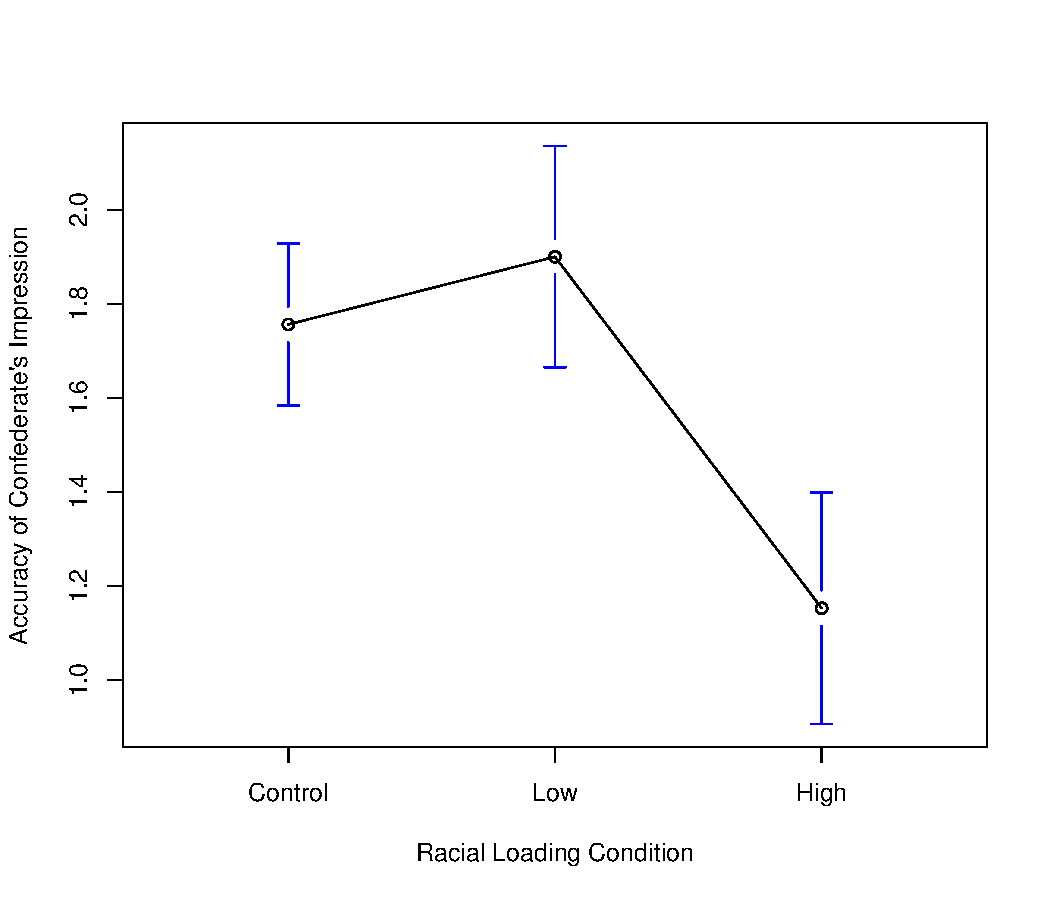
\includegraphics{ReCenterPsychStats_files/figure-latex/unnamed-chunk-101-1.pdf}

With table and figure at hand, here is how I would write up these results:

A one-way analysis of variance was conducted to evaluate the relationship between degree of racial loading of an exceptionalizing microaggression and the perceived accuracy of a research confederate's impression of the Asian or Asian American participant. The independent variable, COND, included three levels: control/none, low, and high levels of racial loading. Results of Levene's homogeneity of variance test indicated no violation of the homogeneity of variance assumption (\(F\){[}2,87{]} = 1.532, \(p\) = 0.222). Similarly, results of the Shapiro Wilk's test indicated no violation of the normality assumption in each of the cells (Control, \emph{W} = 0.954, \emph{p} = 0.215; Low, \emph{W} = 0.944, \emph{p} = 0.115; High, \emph{W} = 0.980, \emph{p} = 0.831).

Results indicated a significant effect of COND on accuracy perception \emph{F} (2, 87) = 13.566, \emph{p} \textless{} .001, \(\eta^2\) = 0.238. In a series of post-hoc comparisons, there were statistically significant differences between the control and high (\(M_{diff}\) = 0.61, \emph{p} \textless{} .001) and low and high (\(M_{diff}\) = 0.75, \emph{p} \textless{} 0.001) conditions, but not the control and low conditions (\(M_{diff}\) = -.14, \emph{p} = 0.347). A statistically significant polynomial contrast suggested a quadratic trend across the three, ordered, levels of the conditions (\(t[87] = -0.364, p = .001\)) such that perception of accuracy increased slighty from the control to low conditions, but decreased more dramatically from low to high. Consequently, it appeared that only the highest degree of racial loading (e.g., ``You speak English well for an Asian'') resulted in the decreased perceptions of accuracy of impressions from the confederate. Means and standard deviations are presented in Table 1 and complete ANOVA results are presented in Table 2. Figure 1 provides an illustration of the results.

\hypertarget{a-conversation-with-dr.-tran}{%
\section{A Conversation with Dr.~Tran}\label{a-conversation-with-dr.-tran}}

Doctoral student (and Teaching Assistant for one of my classes) Jadvir Gill and I were able to interview the first author (Alisia Tran, PhD) about the article and what it means. Here's a direct \href{https://spu.hosted.panopto.com/Panopto/Pages/Viewer.aspx?id=643f8a1e-bb6d-4ceb-a860-aeba01522528}{link} to that interview.

Among others, we asked:

\begin{itemize}
\tightlist
\item
  What were unexpected challenges to the research method or statistical analysis?
\item
  What were the experiences of the confederates as they offered the statements in teh racial loading conditions? And in the debriefings, did the research participants share anything more anecdotally in their experiences as research participants?
\item
  What are your current ideas about interventions or methods for mitigating the harm caused by racial microaggressions?
\item
  How do you expect the article to change science, practice, and/or advocacy?
\end{itemize}

\hypertarget{practice-problems-1}{%
\section{Practice Problems}\label{practice-problems-1}}

In each of these lessons I provide suggestions for practice that allow you to select one or more problems that offer differing levels of difficulty. Whichever you choose, you will focus on these larger steps in one-way ANOVA, including:

\begin{itemize}
\tightlist
\item
  testing the statistical assumptions
\item
  conducting a one-way ANOVA, including

  \begin{itemize}
  \tightlist
  \item
    omnibus test and effect size
  \item
    follow-up (pairwise, planned comparisons, polynomial trends)
  \end{itemize}
\item
  writing a results section to include a figure and tables
\end{itemize}

\hypertarget{problem-1-play-around-with-this-simulation.}{%
\subsection{Problem \#1: Play around with this simulation.}\label{problem-1-play-around-with-this-simulation.}}

If one-way ANOVA is new to you, perhaps you just change the number in ``set.seed(2021)'' from 2021 to something else. Your results should parallel those obtained in the lecture, making it easier for you to check your work as you go.

There are other ways to change the dataset. For example, if you are interested in power, change the sample size to something larger or smaller. If you are interested in variability (i.e., the homogeneity of variance assumption), perhaps you change the standard deviations in a way that violates the assumption.

\hypertarget{problem-2-conduct-a-one-way-anova-with-the-moretalk-dependent-variable.}{%
\subsection{\texorpdfstring{Problem \#2: Conduct a one-way ANOVA with the \emph{moreTalk} dependent variable.}{Problem \#2: Conduct a one-way ANOVA with the moreTalk dependent variable.}}\label{problem-2-conduct-a-one-way-anova-with-the-moretalk-dependent-variable.}}

In their study, Tran and Lee \citeyearpar{tran_you_2014} included an outcome variable where participants rated how much longer they would continue the interaction with their partner compared to their interactions in general. The scale ranged from -2 (\emph{much less than average}) through 0 (\emph{average}) to 2 (\emph{much more than average}). This variable is available in the original simulation and is an option for a slightly more challenging analysis.

\hypertarget{problem-3-try-something-entirely-new.}{%
\subsection{Problem \#3: Try something entirely new.}\label{problem-3-try-something-entirely-new.}}

Using data for which you have permission and access (e.g., IRB approved data you have collected or from your lab; data you simulate from a published article; data from an open science repository; data from other chapters in this OER), complete a one-way ANOVA. Please have at least 3 levels for the predictor variable.

\hypertarget{grading-rubric-1}{%
\subsection{Grading Rubric}\label{grading-rubric-1}}

Regardless which option(s) you chose, use the elements in the grading rubric to guide you through the practice.

\begin{longtable}[]{@{}
  >{\raggedright\arraybackslash}p{(\columnwidth - 4\tabcolsep) * \real{0.5493}}
  >{\centering\arraybackslash}p{(\columnwidth - 4\tabcolsep) * \real{0.2535}}
  >{\centering\arraybackslash}p{(\columnwidth - 4\tabcolsep) * \real{0.1972}}@{}}
\toprule
\begin{minipage}[b]{\linewidth}\raggedright
Assignment Component
\end{minipage} & \begin{minipage}[b]{\linewidth}\centering
Points Possible
\end{minipage} & \begin{minipage}[b]{\linewidth}\centering
Points Earned
\end{minipage} \\
\midrule
\endhead
1. Narrate the research vignette, describing the IV and DV & 5 & \_\_\_\_\_ \\
2. Simulate (or import) and format data & 5 & \_\_\_\_\_ \\
3. Evaluate statistical assumptions & 5 & \_\_\_\_\_ \\
4. Conduct omnibus ANOVA (w effect size) & 5 & \_\_\_\_\_ \\
5. Conduct one set of follow-up tests; narrate your choice & 5 & \_\_\_\_\_ \\
6. Describe approach for managing Type I error & 5 & \_\_\_\_\_ \\
7. APA style results with table(s) and figure & 5 & \_\_\_\_\_ \\
8 Explanation to grader & 5 & \_\_\_\_\_ \\
\textbf{Totals} & 40 & \_\_\_\_\_ \\
\bottomrule
\end{longtable}

\hypertarget{bonus-reel}{%
\section{Bonus Reel:}\label{bonus-reel}}

\begin{figure}
\hypertarget{id}{%
\centering
\includegraphics[width=6.45833in,height=2.19792in]{images/film-strip-1.jpg}
\caption{Image of a filmstrip signifying that the what follows is considered to be supplemental}\label{id}
}
\end{figure}

\hypertarget{whats-with-the-inline-code}{%
\subsection{What's with the inline code?}\label{whats-with-the-inline-code}}

If you are working in the .rmd file you may notice sections that look like this:

\begin{Shaded}
\begin{Highlighting}[]
\CommentTok{\# this script is used for the inline coding in the lesson and,}
\CommentTok{\# although you will want to run it so you can \textquotesingle{}feed\textquotesingle{} the objects into}
\CommentTok{\# later script, there is no \textquotesingle{}lesson\textquotesingle{} relative to this lecture}
\NormalTok{df1omnibus }\OtherTok{\textless{}{-}}\NormalTok{ formattable}\SpecialCharTok{::}\FunctionTok{digits}\NormalTok{(}\FunctionTok{summary}\NormalTok{(omnibus)[[}\DecValTok{1}\NormalTok{]][}\DecValTok{1}\NormalTok{, }\StringTok{"Df"}\NormalTok{], }\DecValTok{0}\NormalTok{)}
\NormalTok{df1omnibus}
\NormalTok{df2omnibus }\OtherTok{\textless{}{-}}\NormalTok{ formattable}\SpecialCharTok{::}\FunctionTok{digits}\NormalTok{(}\FunctionTok{summary}\NormalTok{(omnibus)[[}\DecValTok{1}\NormalTok{]][}\DecValTok{2}\NormalTok{, }\StringTok{"Df"}\NormalTok{], }\DecValTok{0}\NormalTok{)}
\NormalTok{df2omnibus}
\NormalTok{SSMomnibus }\OtherTok{\textless{}{-}}\NormalTok{ formattable}\SpecialCharTok{::}\FunctionTok{digits}\NormalTok{(}\FunctionTok{summary}\NormalTok{(omnibus)[[}\DecValTok{1}\NormalTok{]][}\DecValTok{1}\NormalTok{, }\StringTok{"Sum Sq"}\NormalTok{], }\DecValTok{3}\NormalTok{)}
\NormalTok{SSMomnibus}
\NormalTok{SSRomnibus }\OtherTok{\textless{}{-}}\NormalTok{ formattable}\SpecialCharTok{::}\FunctionTok{digits}\NormalTok{(}\FunctionTok{summary}\NormalTok{(omnibus)[[}\DecValTok{1}\NormalTok{]][}\DecValTok{2}\NormalTok{, }\StringTok{"Sum Sq"}\NormalTok{], }\DecValTok{3}\NormalTok{)}
\NormalTok{SSRomnibus}
\NormalTok{SSTomnibus }\OtherTok{\textless{}{-}}\NormalTok{ formattable}\SpecialCharTok{::}\FunctionTok{digits}\NormalTok{((SSMomnibus }\SpecialCharTok{+}\NormalTok{ SSRomnibus), }\DecValTok{3}\NormalTok{)}
\NormalTok{SSTomnibus}
\NormalTok{MSMomnibus }\OtherTok{\textless{}{-}}\NormalTok{ formattable}\SpecialCharTok{::}\FunctionTok{digits}\NormalTok{(}\FunctionTok{summary}\NormalTok{(omnibus)[[}\DecValTok{1}\NormalTok{]][}\DecValTok{1}\NormalTok{, }\StringTok{"Mean Sq"}\NormalTok{],}
    \DecValTok{3}\NormalTok{)}
\NormalTok{MSMomnibus}
\NormalTok{MSRomnibus }\OtherTok{\textless{}{-}}\NormalTok{ formattable}\SpecialCharTok{::}\FunctionTok{digits}\NormalTok{(}\FunctionTok{summary}\NormalTok{(omnibus)[[}\DecValTok{1}\NormalTok{]][}\DecValTok{2}\NormalTok{, }\StringTok{"Mean Sq"}\NormalTok{],}
    \DecValTok{3}\NormalTok{)}
\NormalTok{MSRomnibus}
\NormalTok{Fomnibus }\OtherTok{\textless{}{-}}\NormalTok{ formattable}\SpecialCharTok{::}\FunctionTok{digits}\NormalTok{(}\FunctionTok{summary}\NormalTok{(omnibus)[[}\DecValTok{1}\NormalTok{]][}\DecValTok{1}\NormalTok{, }\StringTok{"F value"}\NormalTok{], }\DecValTok{3}\NormalTok{)}
\NormalTok{Fomnibus}
\NormalTok{pomnibus }\OtherTok{\textless{}{-}}\NormalTok{ formattable}\SpecialCharTok{::}\FunctionTok{digits}\NormalTok{(}\FunctionTok{summary}\NormalTok{(omnibus)[[}\DecValTok{1}\NormalTok{]][}\DecValTok{1}\NormalTok{, }\StringTok{"Pr(\textgreater{}F)"}\NormalTok{], }\DecValTok{3}\NormalTok{)}
\NormalTok{pomnibus}
\end{Highlighting}
\end{Shaded}

I'm still learning about this and am using the lessons to practice. In these hidden (from the rendered view) boxes of script, I am capturing the output values as R objects. Later I can use inline code (the object's name, preceded with an ``r'', surrounded by tics {[}unfortunately, I cannot demo it in the .rmd file without getting an error{]}) to insert the value into the lecture notes and results. I'm working up to writing an entire journal article in R. This way, if something changes (e.g., more participants in the Qualtrics survey, a different approach to cleaning data) when I re-run the script everything auto-updates and I'm at less of a risk (or maybe a different kind of risk) for making typographical errors.

\hypertarget{between}{%
\chapter{Factorial (Between-Subjects) ANOVA}\label{between}}

\href{https://spu.hosted.panopto.com/Panopto/Pages/Viewer.aspx?pid=3bb1bee1-c2ac-4cda-95f2-ad8b0152132c}{Screencasted Lecture Link}

In this (somewhat long and complex) lesson we conduct a 3X2 ANOVA. We will

\begin{itemize}
\tightlist
\item
  Work an actual example from the literature.

  \begin{itemize}
  \tightlist
  \item
    ``by hand'', and
  \item
    with R packages
  \end{itemize}
\item
  I will also demonstrate

  \begin{itemize}
  \tightlist
  \item
    several options for exploring interaction effects, and
  \item
    several options for exploring main effects.
  \end{itemize}
\item
  Exploring these options will allow us to:

  \begin{itemize}
  \tightlist
  \item
    Gain familiarity with the concepts central to multi-factor ANOVAs.
  \item
    Explore tools for analyzing the complexity in designs.
  \end{itemize}
\end{itemize}

The complexity is that not all of these things need to be conducted for every analysis. The Two-Way ANOVA Workflow is provided to help you map a way through your own analyses. I will periodically refer to this map so that we can more easily keep track of where we are in the process.

\hypertarget{navigating-this-lesson-3}{%
\section{Navigating this Lesson}\label{navigating-this-lesson-3}}

There is about 1 hour and 30 minutes hours of lecture. If you work through the materials with me plan for another two hours of study.

While the majority of R objects and data you will need are created within the R script that sources the chapter, occasionally there are some that cannot be created from within the R framework. Additionally, sometimes links fail. All original materials are provided at the \href{https://github.com/lhbikos/ReCenterPsychStats}{Github site} that hosts the book. More detailed guidelines for ways to access all these materials are provided in the OER's \protect\hyperlink{ReCintro}{introduction}

\hypertarget{learning-objectives-3}{%
\subsection{Learning Objectives}\label{learning-objectives-3}}

Learning objectives from this lecture include the following:

\begin{itemize}
\tightlist
\item
  Define, locate, and interpret all the effects associated with two-way ANOVA:

  \begin{itemize}
  \tightlist
  \item
    main
  \item
    interaction (introducing the concept, \emph{moderator})
  \item
    simple main effects
  \end{itemize}
\item
  Identify which means belong with which effects. Then compare and interpret them.

  \begin{itemize}
  \tightlist
  \item
    marginal means
  \item
    individual cell means
  \item
    comparing them
  \end{itemize}
\item
  Map a process/workflow for investigating a factorial ANOVA
\item
  Manage Type I error
\item
  Conduct a power analysis to determine sample size
\end{itemize}

\hypertarget{planning-for-practice-2}{%
\subsection{Planning for Practice}\label{planning-for-practice-2}}

In each of these lessons I provide suggestions for practice that allow you to select one or more problems that are graded in difficulty The least complex is to change the random seed and rework the problem demonstrated in the lesson. The results \emph{should} map onto the ones obtained in the lecture.

The second option comes from the research vignette. The Ramdhani et al. \citeyearpar{ramdhani_affective_2018} article has two dependent variables (DVs; negative and positive evaluation) which are suitable for two-way ANOVAs. I will demonstrate a simulation of one of their 3X2 ANOVAs (negative) in this lecturette. The second dependent variable (positive) is suggested for the moderate level of difficulty.

As a third option, you are welcome to use data to which you have access and is suitable for two-way ANOVA. In either case the practice options suggest that you:

\begin{itemize}
\tightlist
\item
  test the statistical assumptions
\item
  conduct a two-way ANOVA, including

  \begin{itemize}
  \tightlist
  \item
    omnibus test and effect size
  \item
    report main and interaction effects
  \item
    conduct follow-up testing of simple main effects
  \end{itemize}
\item
  write a results section to include a figure and tables
\end{itemize}

\hypertarget{readings-resources-2}{%
\subsection{Readings \& Resources}\label{readings-resources-2}}

In preparing this chapter, I drew heavily from the following resource(s) that are freely available on the internet. Other resources are cited (when possible, linked) in the text with complete citations in the reference list.

\begin{itemize}
\tightlist
\item
  Navarro, D. (2020). Chapter 16: Factorial ANOVA. In \href{https://learningstatisticswithr.com/}{Learning Statistics with R - A tutorial for Psychology Students and other Beginners}. Retrieved from \url{https://stats.libretexts.org/Bookshelves/Applied_Statistics/Book\%3A_Learning_Statistics_with_R_-_A_tutorial_for_Psychology_Students_and_other_Beginners_(Navarro)}

  \begin{itemize}
  \tightlist
  \item
    Navarro's OER includes a good mix of conceptual information about one-way ANOVA as well as R code. My code/approach is a mix of Green and Salkind's \citeyearpar{green_using_2014}, Field's \citeyearpar{field_discovering_2012}, Navarro's \citeyearpar{navarro_chapter_2020}, and other techniques I have found on the internet and learned from my students.
  \end{itemize}
\item
  Ramdhani, N., Thontowi, H. B., \& Ancok, D. (2018). Affective Reactions Among Students Belonging to Ethnic Groups Engaged in Prior Conflict. \emph{Journal of Pacific Rim Psychology, 12}, e2. \url{https://doi.org/10.1017/prp.2017.22}

  \begin{itemize}
  \tightlist
  \item
    The source of our research vignette.
  \end{itemize}
\end{itemize}

\hypertarget{packages-1}{%
\subsection{Packages}\label{packages-1}}

The packages used in this lesson are embedded in this code. When the hashtags are removed, the script below will (a) check to see if the following packages are installed on your computer and, if not (b) install them.

\begin{Shaded}
\begin{Highlighting}[]
\CommentTok{\# will install the package if not already installed}
\CommentTok{\# if(!require(knitr))\{install.packages(\textquotesingle{}knitr\textquotesingle{})\}}
\CommentTok{\# if(!require(psych))\{install.packages(\textquotesingle{}psych\textquotesingle{})\}}
\CommentTok{\# if(!require(tidyverse))\{install.packages(\textquotesingle{}tidyverse\textquotesingle{})\}}
\CommentTok{\# if(!require(lsr))\{install.packages(\textquotesingle{}lsr\textquotesingle{})\}}
\CommentTok{\# if(!require(car))\{install.packages(\textquotesingle{}car\textquotesingle{})\}}
\CommentTok{\# if(!require(ggpubr))\{install.packages(\textquotesingle{}ggpubr\textquotesingle{})\}}
\CommentTok{\# if(!require(effectsize))\{install.packages(\textquotesingle{}effectsize\textquotesingle{})\}}
\CommentTok{\# if(!require(pwr2))\{install.packages(\textquotesingle{}pwr2\textquotesingle{})\}}
\CommentTok{\# if(!require(apaTables))\{install.packages(\textquotesingle{}apaTables\textquotesingle{})\}}
\end{Highlighting}
\end{Shaded}

\hypertarget{introducing-factorial-anova}{%
\section{Introducing Factorial ANOVA}\label{introducing-factorial-anova}}

My approach to teaching is to address the conceptual as we work problems. That said, there are some critical ideas we should address first.

\textbf{ANOVA is for experiments} (or arguably closely related designs). As we get into the assumptions you'll see that it has some rather restrictive ones (e.g., there should be an equal/equivalent number of cases per cell). To the degree that we violate these assumptions, we should locate alternative statistical approaches where these assumptions are relaxed.

\textbf{Factorial}: a term used when there are two or more independent variables (IVs; the factors). The factors could be between-groups, within-groups, repeated measures, or a combination of between and within.

\begin{itemize}
\tightlist
\item
  \textbf{Independent factorial design}: several IVs (predictors/factors) and each has been measured using different participants (between groups).
\item
  \textbf{Related factorial design}: several IVs (factors/predictors) have been measured, but the same participants have been used in all conditions (repeated measures or within-subjects).
\item
  \textbf{Mixed design}: several IVs (factors/predictors) have been measured. One or more factors uses different participants (between-subjects) and one or more factors uses the same participants (within-subjects). Thus, there is a cobination of independent (between) and related (within or repated) designs.
\item
  Factor naming follows a number/levels convention.
\item
  Today's example is a 3X2 ANOVA. We know there are two factors that have three and two levels, respectively: \emph{ethnicity} has three levels representing the two ethnic groups that were in prior conflict (Marudese, Dayaknese) and a third group who was uninvolved in the conflict (Javanese); \emph{photo stimulus} has two levels representing members of the two ethnic groups that were in prior conflict (Madurese, Dayaknese);
\end{itemize}

\textbf{Moderator} is what creates an interaction. Below are traditional representations of the \emph{statistical} and \emph{conceptual} figures of interaction effects. We will say that Factor B, \emph{moderates} the relationship between Factor A/IV and the DV.

In a later lesson we work an ANCOVA -- where we will distinguish between a \emph{moderator} and a \emph{covariate.} In regression models, you will likely be introduced to the \emph{mediator.}

\begin{figure}
\centering
\includegraphics{images/factorial/modfigs.jpg}
\caption{Graphic representations of a moderated relationship?}
\end{figure}

\hypertarget{workflow-for-two-way-anova}{%
\subsection{Workflow for Two-Way ANOVA}\label{workflow-for-two-way-anova}}

The following is a proposed workflow for conducting a two-way ANOVA.

\begin{figure}
\centering
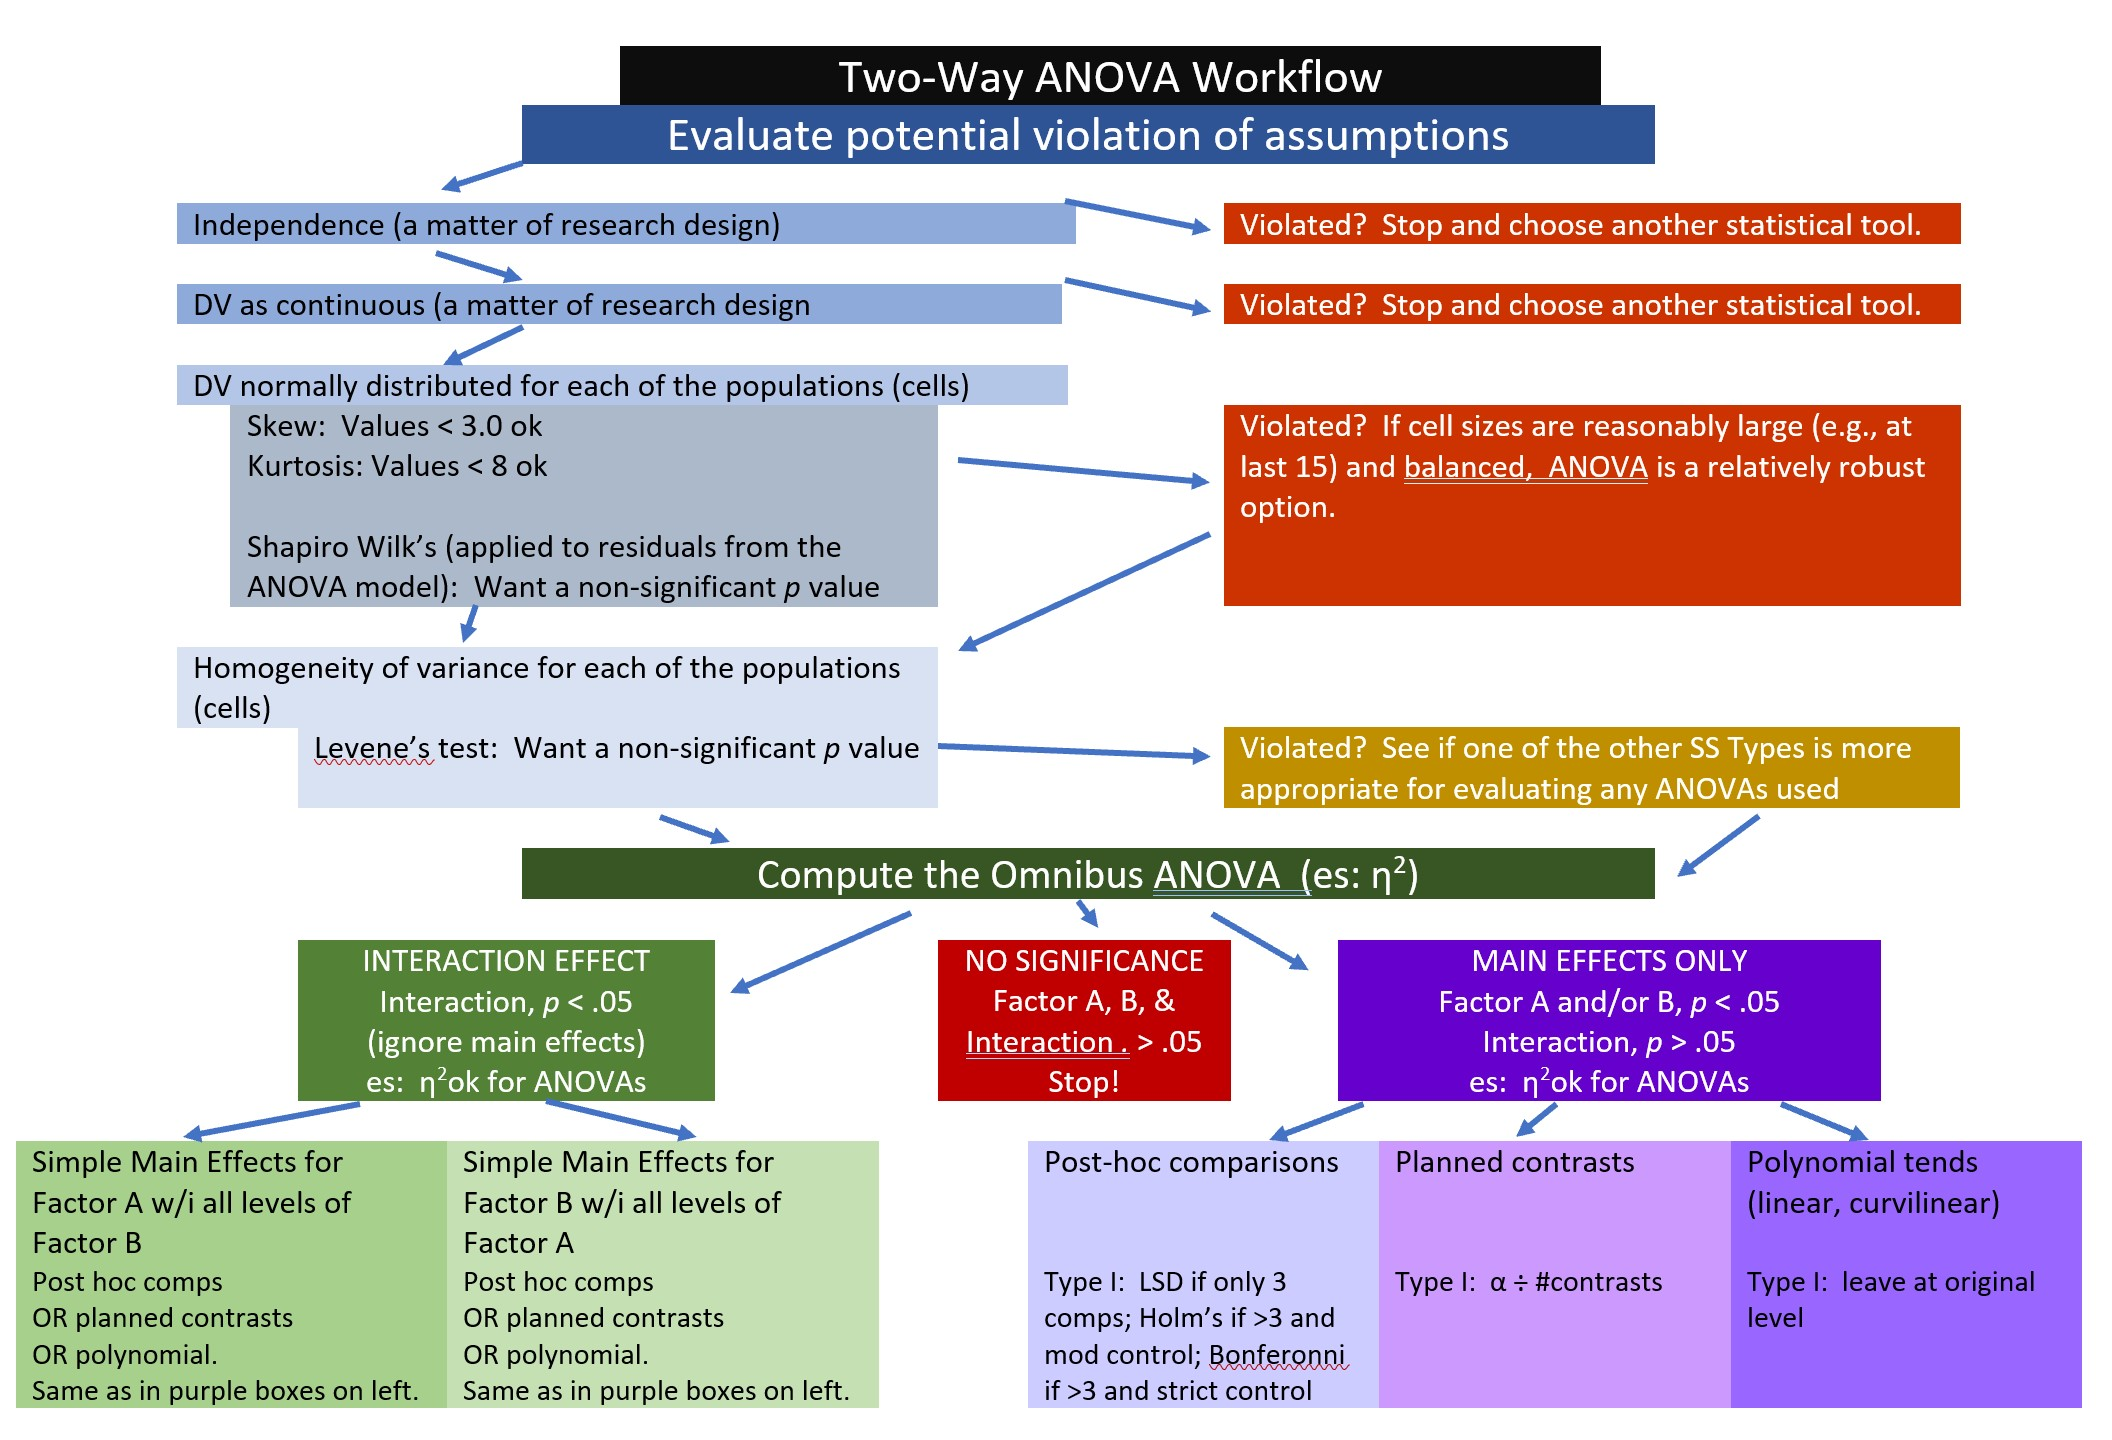
\includegraphics{images/factorial/TwoWayWrkFlo.jpg}
\caption{An image of a workflow for the two-way ANOVA}
\end{figure}

Steps of the workflow include:

\begin{enumerate}
\def\labelenumi{\arabic{enumi}.}
\tightlist
\item
  Enter data

  \begin{itemize}
  \tightlist
  \item
    predictors should formatted as as factors (ordered or unordered); the dependent variable should be continuously scaled
  \item
    understanding the format of data can often provide clues as to which ANOVA/statistic to use
  \end{itemize}
\item
  Explore data

  \begin{itemize}
  \tightlist
  \item
    graphing the data
  \item
    computing descriptive statistics
  \item
    check distributional assumptions
  \item
    use Levene's test to check for homogeneity of variance
  \item
    use Shapiro Wilks to check for normality
  \end{itemize}
\item
  Construct or choose contrasts

  \begin{itemize}
  \tightlist
  \item
    select contrasts and specify for all of the IVs in the analysis
  \item
    if you want to use Type III sums of squares, contrasts must be orthogonal
  \end{itemize}
\item
  Compute the omnibus ANOVA

  \begin{itemize}
  \tightlist
  \item
    \emph{depending on what you found in the data exploration phase, you may need to run a robust version of the test}
  \end{itemize}
\item
  Follow-up testing based on significant main or interaction effects

  \begin{itemize}
  \tightlist
  \item
    significant interactions require test of simple main effects which could be further explored with contrasts, posthoc comparisons, and/or polynomials
  \item
    \emph{the exact methods you choose will depend upon the tests of assumptions during data exploration}
  \end{itemize}
\item
  Managing Type I error
\end{enumerate}

\hypertarget{research-vignette-2}{%
\section{Research Vignette}\label{research-vignette-2}}

The research vignette for this example was located in Kalimantan, Indonesia and focused on bias in young people from three ethnic groups. The Madurese and Dayaknese groups were engaged in ethnic conflict that spanned 1996 to 2001. The last incidence of mass violence was in 2001 where approximately 500 people (mostly from the Madurese ethnic group) were expelled from the province. Ramdhani et al.'s \citeyearpar{ramdhani_affective_2018} research hypotheses were based on the roles of the three ethnic groups in the study. The Madurese appear to be viewed as the transgressors when they occupied lands and took employment and business opportunities from the Dayaknese. Ramdhani et al.~also included a third group who were not involved in the conflict (Javanese). The research participants were students studying in Yogyakara who were not involved in the conflict. They included 39 Madurese, 35 Dyaknese, and 37 Javanese; 83 were male and 28 were female.

In the study \citep{ramdhani_affective_2018}, participants viewed facial pictures of three men and three women (in traditional dress) from each ethnic group (6 photos per ethnic group). Participant were asked, ``How do you feel when you see this photo? Please indicate your answers based on your actual feelings.'' Participants responded on a 7-point Likert scale ranging from 1 (\emph{strongly disagree}) to 7 (\emph{strongly agree}). Higher scores indicated ratings of higher intensity on that scale. The two scales included the following words:

\begin{itemize}
\tightlist
\item
  Positive: friendly, kind, helpful, happy
\item
  Negative: disgusting, suspicious, hateful, angry
\end{itemize}

Below is script to simulate data for the negative reactions variable from the information available from the manuscript \citep{ramdhani_affective_2018}.

\begin{Shaded}
\begin{Highlighting}[]
\FunctionTok{library}\NormalTok{(tidyverse)}
\FunctionTok{set.seed}\NormalTok{(}\DecValTok{210731}\NormalTok{)}
\CommentTok{\# sample size, M and SD for each cell; this will put it in a long}
\CommentTok{\# file}
\NormalTok{Negative }\OtherTok{\textless{}{-}} \FunctionTok{round}\NormalTok{(}\FunctionTok{c}\NormalTok{(}\FunctionTok{rnorm}\NormalTok{(}\DecValTok{17}\NormalTok{, }\AttributeTok{mean =} \FloatTok{1.91}\NormalTok{, }\AttributeTok{sd =} \FloatTok{0.73}\NormalTok{), }\FunctionTok{rnorm}\NormalTok{(}\DecValTok{18}\NormalTok{, }\AttributeTok{mean =} \FloatTok{3.16}\NormalTok{,}
    \AttributeTok{sd =} \FloatTok{0.19}\NormalTok{), }\FunctionTok{rnorm}\NormalTok{(}\DecValTok{19}\NormalTok{, }\AttributeTok{mean =} \FloatTok{3.3}\NormalTok{, }\AttributeTok{sd =} \FloatTok{1.05}\NormalTok{), }\FunctionTok{rnorm}\NormalTok{(}\DecValTok{20}\NormalTok{, }\AttributeTok{mean =} \DecValTok{3}\NormalTok{, }\AttributeTok{sd =} \FloatTok{1.07}\NormalTok{),}
    \FunctionTok{rnorm}\NormalTok{(}\DecValTok{18}\NormalTok{, }\AttributeTok{mean =} \FloatTok{2.64}\NormalTok{, }\AttributeTok{sd =} \FloatTok{0.95}\NormalTok{), }\FunctionTok{rnorm}\NormalTok{(}\DecValTok{19}\NormalTok{, }\AttributeTok{mean =} \FloatTok{2.99}\NormalTok{, }\AttributeTok{sd =} \FloatTok{0.8}\NormalTok{)),}
    \DecValTok{3}\NormalTok{)}
\CommentTok{\# sample size, M and SD for each cell; this will put it in a long}
\CommentTok{\# file}
\NormalTok{Positive }\OtherTok{\textless{}{-}} \FunctionTok{round}\NormalTok{(}\FunctionTok{c}\NormalTok{(}\FunctionTok{rnorm}\NormalTok{(}\DecValTok{17}\NormalTok{, }\AttributeTok{mean =} \FloatTok{4.99}\NormalTok{, }\AttributeTok{sd =} \FloatTok{1.38}\NormalTok{), }\FunctionTok{rnorm}\NormalTok{(}\DecValTok{18}\NormalTok{, }\AttributeTok{mean =} \FloatTok{3.83}\NormalTok{,}
    \AttributeTok{sd =} \FloatTok{1.13}\NormalTok{), }\FunctionTok{rnorm}\NormalTok{(}\DecValTok{19}\NormalTok{, }\AttributeTok{mean =} \FloatTok{4.2}\NormalTok{, }\AttributeTok{sd =} \FloatTok{0.82}\NormalTok{), }\FunctionTok{rnorm}\NormalTok{(}\DecValTok{20}\NormalTok{, }\AttributeTok{mean =} \FloatTok{4.19}\NormalTok{,}
    \AttributeTok{sd =} \FloatTok{0.91}\NormalTok{), }\FunctionTok{rnorm}\NormalTok{(}\DecValTok{18}\NormalTok{, }\AttributeTok{mean =} \FloatTok{4.17}\NormalTok{, }\AttributeTok{sd =} \FloatTok{0.6}\NormalTok{), }\FunctionTok{rnorm}\NormalTok{(}\DecValTok{19}\NormalTok{, }\AttributeTok{mean =} \FloatTok{3.26}\NormalTok{,}
    \AttributeTok{sd =} \FloatTok{0.94}\NormalTok{)), }\DecValTok{3}\NormalTok{)}
\NormalTok{ID }\OtherTok{\textless{}{-}} \FunctionTok{factor}\NormalTok{(}\FunctionTok{seq}\NormalTok{(}\DecValTok{1}\NormalTok{, }\DecValTok{111}\NormalTok{))}
\NormalTok{Rater }\OtherTok{\textless{}{-}} \FunctionTok{c}\NormalTok{(}\FunctionTok{rep}\NormalTok{(}\StringTok{"Dayaknese"}\NormalTok{, }\DecValTok{35}\NormalTok{), }\FunctionTok{rep}\NormalTok{(}\StringTok{"Madurese"}\NormalTok{, }\DecValTok{39}\NormalTok{), }\FunctionTok{rep}\NormalTok{(}\StringTok{"Javanese"}\NormalTok{, }\DecValTok{37}\NormalTok{))}
\NormalTok{Photo }\OtherTok{\textless{}{-}} \FunctionTok{c}\NormalTok{(}\FunctionTok{rep}\NormalTok{(}\StringTok{"Dayaknese"}\NormalTok{, }\DecValTok{17}\NormalTok{), }\FunctionTok{rep}\NormalTok{(}\StringTok{"Madurese"}\NormalTok{, }\DecValTok{18}\NormalTok{), }\FunctionTok{rep}\NormalTok{(}\StringTok{"Dayaknese"}\NormalTok{,}
    \DecValTok{19}\NormalTok{), }\FunctionTok{rep}\NormalTok{(}\StringTok{"Madurese"}\NormalTok{, }\DecValTok{20}\NormalTok{), }\FunctionTok{rep}\NormalTok{(}\StringTok{"Dayaknese"}\NormalTok{, }\DecValTok{18}\NormalTok{), }\FunctionTok{rep}\NormalTok{(}\StringTok{"Madurese"}\NormalTok{, }\DecValTok{19}\NormalTok{))}
\CommentTok{\# groups the 3 variables into a single df: ID\#, DV, condition}
\NormalTok{Ramdhani\_df }\OtherTok{\textless{}{-}} \FunctionTok{data.frame}\NormalTok{(ID, Negative, Positive, Rater, Photo)}
\end{Highlighting}
\end{Shaded}

For two-way ANOVA our variables need to be properly formatted. In our case:

\begin{itemize}
\tightlist
\item
  Negative is a continuously scaled DV and should be \emph{num}
\item
  Positive is a continuously scaled DV and should be \emph{num}
\item
  Rater should be an unordered factor
\item
  Photo should be an unordered facor
\end{itemize}

\begin{Shaded}
\begin{Highlighting}[]
\FunctionTok{str}\NormalTok{(Ramdhani\_df)}
\end{Highlighting}
\end{Shaded}

\begin{verbatim}
'data.frame':   111 obs. of  5 variables:
 $ ID      : Factor w/ 111 levels "1","2","3","4",..: 1 2 3 4 5 6 7 8 9 10 ...
 $ Negative: num  2.768 1.811 0.869 1.857 2.087 ...
 $ Positive: num  5.91 5.23 3.54 5.63 5.44 ...
 $ Rater   : chr  "Dayaknese" "Dayaknese" "Dayaknese" "Dayaknese" ...
 $ Photo   : chr  "Dayaknese" "Dayaknese" "Dayaknese" "Dayaknese" ...
\end{verbatim}

Our Negative variable is correctly formatted. Let's reformat Rater and Photo to be factors and ask for the structure again. R's default is to order the factors alphabetically. In this case this is fine. If we had ordered factors such as dosage (placebo, lo, hi) we would want to respecify the order.

\begin{Shaded}
\begin{Highlighting}[]
\NormalTok{Ramdhani\_df[, }\StringTok{"Rater"}\NormalTok{] }\OtherTok{\textless{}{-}} \FunctionTok{as.factor}\NormalTok{(Ramdhani\_df[, }\StringTok{"Rater"}\NormalTok{])}
\NormalTok{Ramdhani\_df[, }\StringTok{"Photo"}\NormalTok{] }\OtherTok{\textless{}{-}} \FunctionTok{as.factor}\NormalTok{(Ramdhani\_df[, }\StringTok{"Photo"}\NormalTok{])}
\FunctionTok{str}\NormalTok{(Ramdhani\_df)}
\end{Highlighting}
\end{Shaded}

\begin{verbatim}
'data.frame':   111 obs. of  5 variables:
 $ ID      : Factor w/ 111 levels "1","2","3","4",..: 1 2 3 4 5 6 7 8 9 10 ...
 $ Negative: num  2.768 1.811 0.869 1.857 2.087 ...
 $ Positive: num  5.91 5.23 3.54 5.63 5.44 ...
 $ Rater   : Factor w/ 3 levels "Dayaknese","Javanese",..: 1 1 1 1 1 1 1 1 1 1 ...
 $ Photo   : Factor w/ 2 levels "Dayaknese","Madurese": 1 1 1 1 1 1 1 1 1 1 ...
\end{verbatim}

If you want to export this data as a file to your computer, remove the hashtags to save it (and re-import it) as a .csv (``Excel lite'') or .rds (R object) file. This is not a necessary step.

The code for .csv will likely lose the formatting (i.e., making the Rater and Photo variables factors), but it is easy to view in Excel.

\begin{Shaded}
\begin{Highlighting}[]
\CommentTok{\# write the simulated data as a .csv write.table(Ramdhani\_df,}
\CommentTok{\# file=\textquotesingle{}RamdhaniCSV.csv\textquotesingle{}, sep=\textquotesingle{},\textquotesingle{}, col.names=TRUE, row.names=FALSE)}
\CommentTok{\# bring back the simulated dat from a .csv file Ramdhani\_df \textless{}{-}}
\CommentTok{\# read.csv (\textquotesingle{}RamdhaniCSV.csv\textquotesingle{}, header = TRUE) str(Ramdhani\_df)}
\end{Highlighting}
\end{Shaded}

The code for the .rds file will retain the formatting of the variables, but is not easy to view outside of R.

\begin{Shaded}
\begin{Highlighting}[]
\CommentTok{\# to save the df as an .rds (think \textquotesingle{}R object\textquotesingle{}) file on your computer;}
\CommentTok{\# it should save in the same file as the .rmd file you are working}
\CommentTok{\# with saveRDS(Ramdhani\_df, \textquotesingle{}Ramdhani\_RDS.rds\textquotesingle{}) bring back the}
\CommentTok{\# simulated dat from an .rds file Ramdhani\_RDS \textless{}{-}}
\CommentTok{\# readRDS(\textquotesingle{}Ramdhani\_RDS.rds\textquotesingle{}) str(Ramdhani\_RDS)}
\end{Highlighting}
\end{Shaded}

\hypertarget{preliminary-exploration-of-our-research-vignette}{%
\subsection{Preliminary exploration of our research vignette}\label{preliminary-exploration-of-our-research-vignette}}

Let's first examine the descriptive statistics (e.g., means of the variable, Negative) by group. We can use the \emph{describeBy()} function from the \emph{psych} package.

\begin{Shaded}
\begin{Highlighting}[]
\NormalTok{negative.descripts }\OtherTok{\textless{}{-}}\NormalTok{ psych}\SpecialCharTok{::}\FunctionTok{describeBy}\NormalTok{(Negative }\SpecialCharTok{\textasciitilde{}}\NormalTok{ Rater }\SpecialCharTok{+}\NormalTok{ Photo, }\AttributeTok{mat =} \ConstantTok{TRUE}\NormalTok{,}
    \AttributeTok{data =}\NormalTok{ Ramdhani\_df, }\AttributeTok{digits =} \DecValTok{3}\NormalTok{)  }\CommentTok{\#digits allows us to round the output}
\NormalTok{negative.descripts}
\end{Highlighting}
\end{Shaded}

\begin{verbatim}
    item    group1    group2 vars  n  mean    sd median trimmed   mad   min
X11    1 Dayaknese Dayaknese    1 17 1.818 0.768  1.692   1.783 0.694 0.706
X12    2  Javanese Dayaknese    1 18 2.524 0.742  2.391   2.460 0.569 1.406
X13    3  Madurese Dayaknese    1 19 3.301 1.030  3.314   3.321 1.294 1.406
X14    4 Dayaknese  Madurese    1 18 3.129 0.156  3.160   3.136 0.104 2.732
X15    5  Javanese  Madurese    1 19 3.465 0.637  3.430   3.456 0.767 2.456
X16    6  Madurese  Madurese    1 20 3.297 1.332  2.958   3.254 1.615 1.211
      max range   skew kurtosis    se
X11 3.453 2.747  0.513   -0.881 0.186
X12 4.664 3.258  1.205    1.475 0.175
X13 4.854 3.448 -0.126   -1.267 0.236
X14 3.423 0.691 -0.623    0.481 0.037
X15 4.631 2.175 -0.010   -1.307 0.146
X16 5.641 4.430  0.215   -1.238 0.298
\end{verbatim}

The \emph{write.table()} function can be a helpful way to export output to .csv files so that you can manipulate it into tables.

\begin{Shaded}
\begin{Highlighting}[]
\FunctionTok{write.table}\NormalTok{(negative.descripts, }\AttributeTok{file =} \StringTok{"NegativeDescripts.csv"}\NormalTok{, }\AttributeTok{sep =} \StringTok{","}\NormalTok{,}
    \AttributeTok{col.names =} \ConstantTok{TRUE}\NormalTok{, }\AttributeTok{row.names =} \ConstantTok{FALSE}\NormalTok{)}
\end{Highlighting}
\end{Shaded}

At this stage, it would be useful to plot our data. Figures can assist in the conceptualization of the analysis.

\begin{Shaded}
\begin{Highlighting}[]
\NormalTok{ggpubr}\SpecialCharTok{::}\FunctionTok{ggboxplot}\NormalTok{(Ramdhani\_df, }\AttributeTok{x =} \StringTok{"Rater"}\NormalTok{, }\AttributeTok{y =} \StringTok{"Negative"}\NormalTok{, }\AttributeTok{color =} \StringTok{"Photo"}\NormalTok{,}
    \AttributeTok{xlab =} \StringTok{"Ethnicity of Rater"}\NormalTok{, }\AttributeTok{ylab =} \StringTok{"Negative Reaction"}\NormalTok{)}
\end{Highlighting}
\end{Shaded}

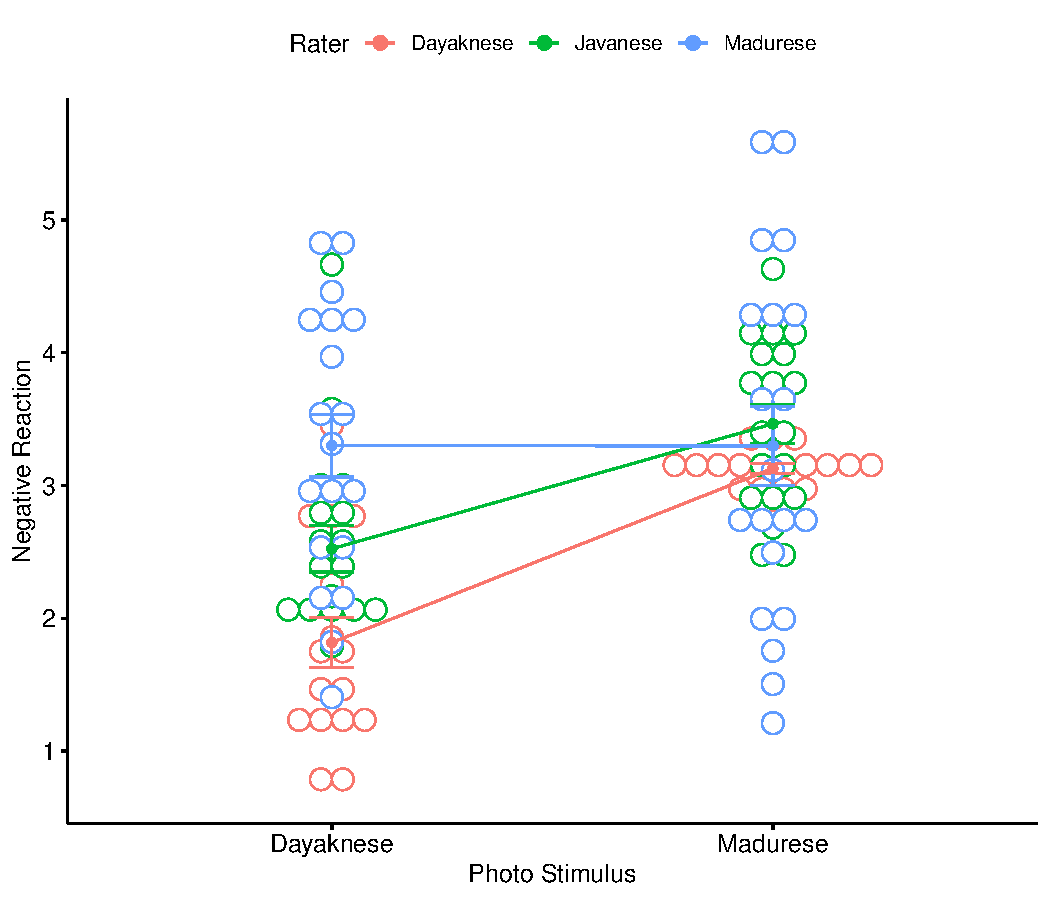
\includegraphics{ReCenterPsychStats_files/figure-latex/unnamed-chunk-113-1.pdf}
Narrating results is sometimes made easier if variables are switched. There is usually not a right or wrong answer. Here is another view, switching the Rater and Photo predictors.

\begin{Shaded}
\begin{Highlighting}[]
\NormalTok{ggpubr}\SpecialCharTok{::}\FunctionTok{ggboxplot}\NormalTok{(Ramdhani\_df, }\AttributeTok{x =} \StringTok{"Photo"}\NormalTok{, }\AttributeTok{y =} \StringTok{"Negative"}\NormalTok{, }\AttributeTok{color =} \StringTok{"Rater"}\NormalTok{,}
    \AttributeTok{xlab =} \StringTok{"Photo Stimulus"}\NormalTok{, }\AttributeTok{ylab =} \StringTok{"Negative Reaction"}\NormalTok{)}
\end{Highlighting}
\end{Shaded}

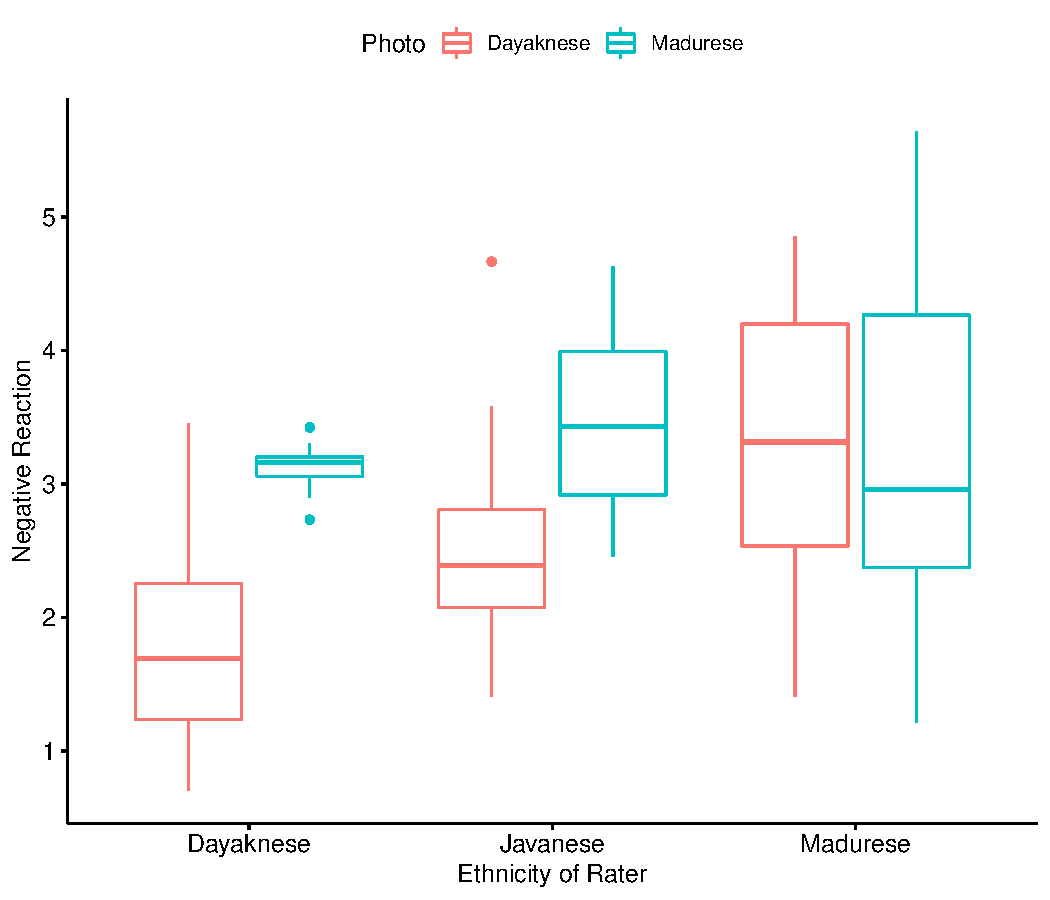
\includegraphics{ReCenterPsychStats_files/figure-latex/unnamed-chunk-114-1.pdf}
Yet another option plots the raw data as bubbles, the means as lines, and denotes differences in the moderator with color.

\begin{Shaded}
\begin{Highlighting}[]
\NormalTok{ggpubr}\SpecialCharTok{::}\FunctionTok{ggline}\NormalTok{(Ramdhani\_df, }\AttributeTok{x =} \StringTok{"Rater"}\NormalTok{, }\AttributeTok{y =} \StringTok{"Negative"}\NormalTok{, }\AttributeTok{color =} \StringTok{"Photo"}\NormalTok{,}
    \AttributeTok{xlab =} \StringTok{"Ethnicity of Rater"}\NormalTok{, }\AttributeTok{ylab =} \StringTok{"Negative Reaction"}\NormalTok{, }\AttributeTok{add =} \FunctionTok{c}\NormalTok{(}\StringTok{"mean\_se"}\NormalTok{,}
        \StringTok{"dotplot"}\NormalTok{))}
\end{Highlighting}
\end{Shaded}

\begin{verbatim}
Bin width defaults to 1/30 of the range of the data. Pick better value with `binwidth`.
\end{verbatim}

\begin{verbatim}
Warning: Computation failed in `stat_summary()`:
object 'mean_se_' of mode 'function' was not found
\end{verbatim}

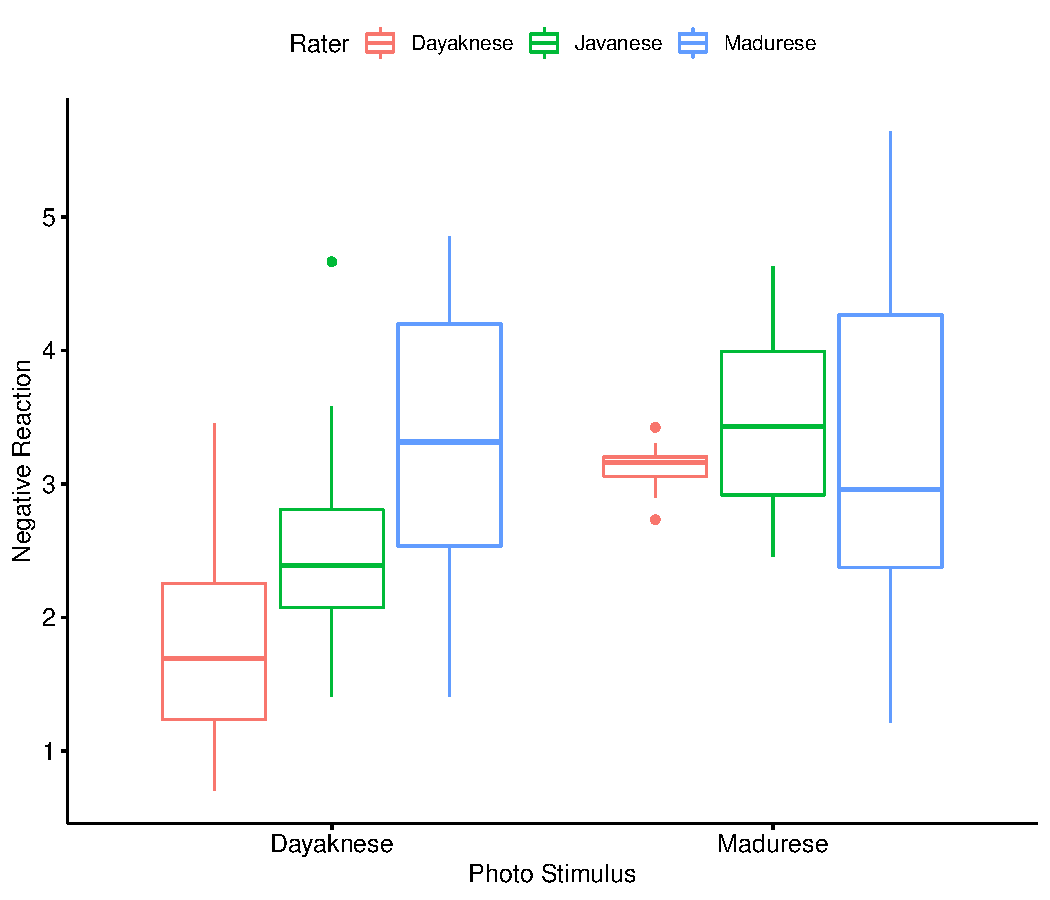
\includegraphics{ReCenterPsychStats_files/figure-latex/unnamed-chunk-115-1.pdf}

\begin{Shaded}
\begin{Highlighting}[]
\CommentTok{\# add this for a different color palette: palette = c(\textquotesingle{}\#00AFBB\textquotesingle{},}
\CommentTok{\# \textquotesingle{}\#E7B800\textquotesingle{})}
\end{Highlighting}
\end{Shaded}

We can reverse this to see if it assists with our conceptualization.

\begin{Shaded}
\begin{Highlighting}[]
\NormalTok{ggpubr}\SpecialCharTok{::}\FunctionTok{ggline}\NormalTok{(Ramdhani\_df, }\AttributeTok{x =} \StringTok{"Photo"}\NormalTok{, }\AttributeTok{y =} \StringTok{"Negative"}\NormalTok{, }\AttributeTok{color =} \StringTok{"Rater"}\NormalTok{,}
    \AttributeTok{xlab =} \StringTok{"Photo Stimulus"}\NormalTok{, }\AttributeTok{ylab =} \StringTok{"Negative Reaction"}\NormalTok{, }\AttributeTok{add =} \FunctionTok{c}\NormalTok{(}\StringTok{"mean\_se"}\NormalTok{,}
        \StringTok{"dotplot"}\NormalTok{))}
\end{Highlighting}
\end{Shaded}

\begin{verbatim}
Bin width defaults to 1/30 of the range of the data. Pick better value with `binwidth`.
\end{verbatim}

\begin{verbatim}
Warning: Computation failed in `stat_summary()`:
object 'mean_se_' of mode 'function' was not found
\end{verbatim}

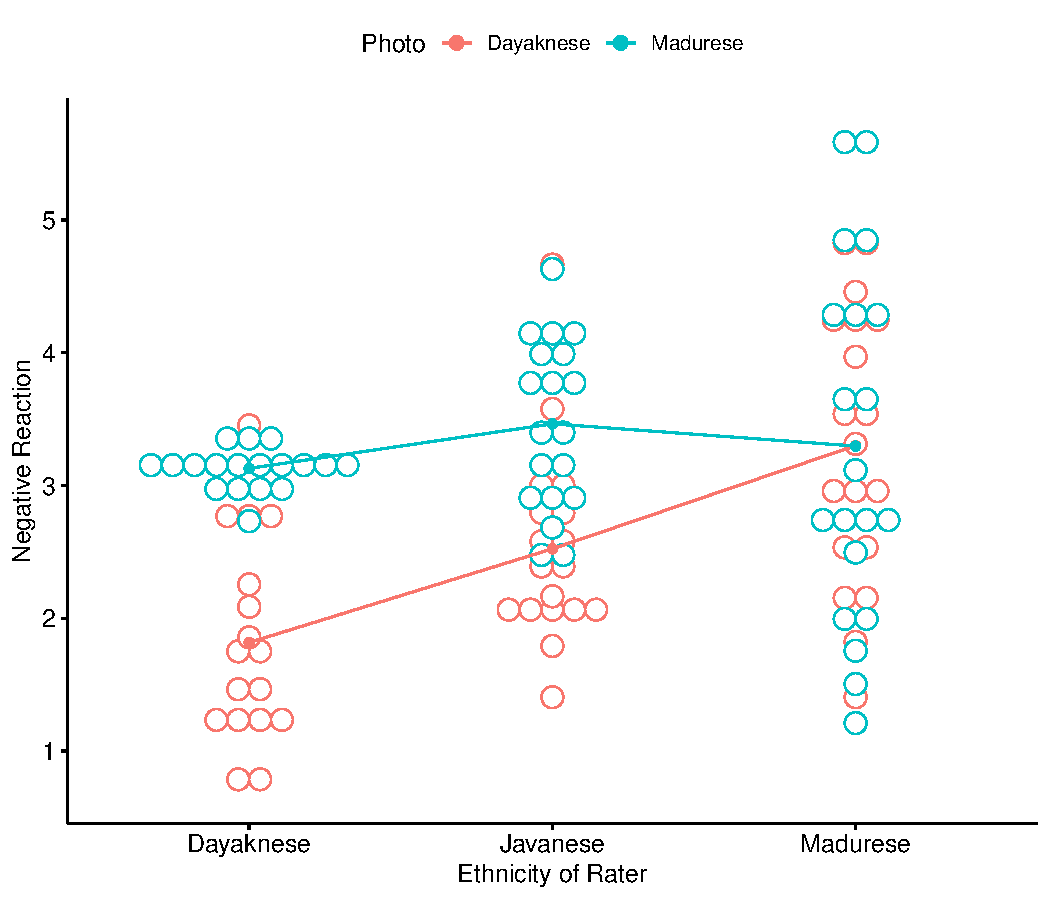
\includegraphics{ReCenterPsychStats_files/figure-latex/unnamed-chunk-116-1.pdf}

\hypertarget{working-the-factorial-anova-by-hand}{%
\section{Working the Factorial ANOVA (by hand)}\label{working-the-factorial-anova-by-hand}}

Before we work an ANOVA let's take a moment to consider what we are doing and how it informs our decision-making. This figure (which already contains ``the answers'') may help conceptualize how variance becomes partitioned.

\begin{figure}
\centering
\includegraphics{images/factorial/partition.png}
\caption{Image of a flowchart that partitions variance from sums of squares totals to its component pieces}
\end{figure}

As in one-way ANOVA, we partition variance into \textbf{total}, \textbf{model}, and \textbf{residual}. However, we now further divide the \(SS_M\) into its respective factors A(column), B(row,) and their a x b product.

In this, we begin to talk about main effects and interactions.

\hypertarget{sums-of-squares-total-1}{%
\subsection{Sums of Squares Total}\label{sums-of-squares-total-1}}

Our formula is the same as it was for one-way ANOVA:

\[SS_{T}= \sum (x_{i}-\bar{x}_{grand})^{2}\]
Let's calculate it for the Ramdhani et al. \citeyearpar{ramdhani_affective_2018} data.
Our grand (i.e., overall) mean is

\begin{Shaded}
\begin{Highlighting}[]
\FunctionTok{mean}\NormalTok{(Ramdhani\_df}\SpecialCharTok{$}\NormalTok{Negative)}
\end{Highlighting}
\end{Shaded}

\begin{verbatim}
[1] 2.947369
\end{verbatim}

Subtracting the grand mean from each Negative rating yields a mean difference.

\begin{Shaded}
\begin{Highlighting}[]
\FunctionTok{library}\NormalTok{(tidyverse)}
\NormalTok{Ramdhani\_df }\OtherTok{\textless{}{-}}\NormalTok{ Ramdhani\_df }\SpecialCharTok{\%\textgreater{}\%}
    \FunctionTok{mutate}\NormalTok{(}\AttributeTok{m\_dev =}\NormalTok{ Negative }\SpecialCharTok{{-}} \FunctionTok{mean}\NormalTok{(Negative))}
\end{Highlighting}
\end{Shaded}

Pop quiz: What's the sum of our new \emph{m\_dev} variable?

Let's find out!

\begin{Shaded}
\begin{Highlighting}[]
\FunctionTok{sum}\NormalTok{(Ramdhani\_df}\SpecialCharTok{$}\NormalTok{m\_dev)}
\end{Highlighting}
\end{Shaded}

\begin{verbatim}
[1] -0.000000000000007549517
\end{verbatim}

Of course! The sum of squared deviations around the mean is zero. Next we square those mean deviations.

\begin{Shaded}
\begin{Highlighting}[]
\NormalTok{Ramdhani\_df }\OtherTok{\textless{}{-}}\NormalTok{ Ramdhani\_df }\SpecialCharTok{\%\textgreater{}\%}
    \FunctionTok{mutate}\NormalTok{(}\AttributeTok{m\_devSQ =}\NormalTok{ m\_dev}\SpecialCharTok{\^{}}\DecValTok{2}\NormalTok{)}
\end{Highlighting}
\end{Shaded}

Then we sum the squared mean deviations.

\begin{Shaded}
\begin{Highlighting}[]
\FunctionTok{sum}\NormalTok{(Ramdhani\_df}\SpecialCharTok{$}\NormalTok{m\_devSQ)}
\end{Highlighting}
\end{Shaded}

\begin{verbatim}
[1] 114.7746
\end{verbatim}

This value, 114.775, the sum of squared deviations around the grand mean, is our \(SS_T\); the associated \emph{degrees of freedom} is \(N\) - 1.

In factorial ANOVA, we divide \(SS_T\) into \textbf{model/between} sums of squares and \textbf{residual/within} sums of squares.

\hypertarget{sums-of-squares-for-the-model}{%
\subsection{Sums of Squares for the Model}\label{sums-of-squares-for-the-model}}

\[SS_{M}= \sum n_{k}(\bar{x}_{k}-\bar{x}_{grand})^{2}\]

The \emph{model} generally represents the notion that the means are different than each other. We want the variation between our means to be greater than the variation within each of the groups from which our means are calculated.

In factorial, we need to obtain means for each of the combinations of the factors. We have a 3 x 2:

\begin{itemize}
\tightlist
\item
  Rater with three levels: Dayaknese, Madurese, Javanese
\item
  Photo with two levels: Dayaknese, Madurese
\end{itemize}

Let's repeat some code we used before to obtain the cell-level means and cell sizes.

\begin{Shaded}
\begin{Highlighting}[]
\NormalTok{psych}\SpecialCharTok{::}\FunctionTok{describeBy}\NormalTok{(Negative }\SpecialCharTok{\textasciitilde{}}\NormalTok{ Rater }\SpecialCharTok{+}\NormalTok{ Photo, }\AttributeTok{mat =} \ConstantTok{TRUE}\NormalTok{, }\AttributeTok{data =}\NormalTok{ Ramdhani\_df,}
    \AttributeTok{digits =} \DecValTok{3}\NormalTok{)}
\end{Highlighting}
\end{Shaded}

\begin{verbatim}
    item    group1    group2 vars  n  mean    sd median trimmed   mad   min
X11    1 Dayaknese Dayaknese    1 17 1.818 0.768  1.692   1.783 0.694 0.706
X12    2  Javanese Dayaknese    1 18 2.524 0.742  2.391   2.460 0.569 1.406
X13    3  Madurese Dayaknese    1 19 3.301 1.030  3.314   3.321 1.294 1.406
X14    4 Dayaknese  Madurese    1 18 3.129 0.156  3.160   3.136 0.104 2.732
X15    5  Javanese  Madurese    1 19 3.465 0.637  3.430   3.456 0.767 2.456
X16    6  Madurese  Madurese    1 20 3.297 1.332  2.958   3.254 1.615 1.211
      max range   skew kurtosis    se
X11 3.453 2.747  0.513   -0.881 0.186
X12 4.664 3.258  1.205    1.475 0.175
X13 4.854 3.448 -0.126   -1.267 0.236
X14 3.423 0.691 -0.623    0.481 0.037
X15 4.631 2.175 -0.010   -1.307 0.146
X16 5.641 4.430  0.215   -1.238 0.298
\end{verbatim}

\begin{Shaded}
\begin{Highlighting}[]
\CommentTok{\# Note. Recently my students and I have been having intermittent}
\CommentTok{\# struggles with the describeBy function in the psych package. We}
\CommentTok{\# have noticed that it is problematic when using .rds files and when}
\CommentTok{\# using data directly imported from Qualtrics. If you are having}
\CommentTok{\# similar difficulties, try uploading the .csv file and making the}
\CommentTok{\# appropriate formatting changes.}
\end{Highlighting}
\end{Shaded}

We also need the grand mean (i.e., the mean that disregards {[}or ``collapses across''{]} the factors).

\begin{Shaded}
\begin{Highlighting}[]
\FunctionTok{mean}\NormalTok{(Ramdhani\_df}\SpecialCharTok{$}\NormalTok{Negative)}
\end{Highlighting}
\end{Shaded}

\begin{verbatim}
[1] 2.947369
\end{verbatim}

This formula occurs in six chunks, representing the six cells of our designed. In each of the chunks we have the \(n\), group mean, and grand mean.

\begin{Shaded}
\begin{Highlighting}[]
\DecValTok{17} \SpecialCharTok{*}\NormalTok{ (}\FloatTok{1.818} \SpecialCharTok{{-}} \FloatTok{2.947}\NormalTok{)}\SpecialCharTok{\^{}}\DecValTok{2} \SpecialCharTok{+} \DecValTok{18} \SpecialCharTok{*}\NormalTok{ (}\FloatTok{2.524} \SpecialCharTok{{-}} \FloatTok{2.947}\NormalTok{)}\SpecialCharTok{\^{}}\DecValTok{2} \SpecialCharTok{+} \DecValTok{19} \SpecialCharTok{*}\NormalTok{ (}\FloatTok{3.301} \SpecialCharTok{{-}} \FloatTok{2.947}\NormalTok{)}\SpecialCharTok{\^{}}\DecValTok{2} \SpecialCharTok{+}
    \DecValTok{18} \SpecialCharTok{*}\NormalTok{ (}\FloatTok{3.129} \SpecialCharTok{{-}} \FloatTok{2.947}\NormalTok{)}\SpecialCharTok{\^{}}\DecValTok{2} \SpecialCharTok{+} \DecValTok{19} \SpecialCharTok{*}\NormalTok{ (}\FloatTok{3.465} \SpecialCharTok{{-}} \FloatTok{2.947}\NormalTok{)}\SpecialCharTok{\^{}}\DecValTok{2} \SpecialCharTok{+} \DecValTok{20} \SpecialCharTok{*}\NormalTok{ (}\FloatTok{3.297} \SpecialCharTok{{-}} \FloatTok{2.947}\NormalTok{)}\SpecialCharTok{\^{}}\DecValTok{2}
\end{Highlighting}
\end{Shaded}

\begin{verbatim}
[1] 35.41501
\end{verbatim}

This value, 35.415, \(SS_M\) is the value accounted for by the model. That is, the amount of variance accounted for by the grouping variable/factors, Rater and Photo.

\hypertarget{sums-of-squares-residual-or-within-1}{%
\subsection{Sums of Squares Residual (or within)}\label{sums-of-squares-residual-or-within-1}}

\(SS_R\) is error associated with within group variability. If people are randomly assigned to treatment group there should be no other covariate (confounding variable) so that all \(SS_R\) variability is \emph{uninteresting} for the research and treated as noise.

\[SS_{R}= \sum(x_{ik}-\bar{x}_{k})^{^{2}}\]
Here's another configuration of the same:

\[SS_{R}= s_{group1}^{2}(n-1) + s_{group2}^{2}(n-1) + s_{group3}^{2}(n-1) + s_{group4}^{2}(n-1) + s_{group5}^{2}(n-1) + s_{group6}^{2}(n-1))\]

Again, the formula is in six chunks -- but this time the calculations are \emph{within-group}. We need the variance (the standard deviation squared) for the calculation. Let's take another look at our descriptives.

\begin{Shaded}
\begin{Highlighting}[]
\NormalTok{psych}\SpecialCharTok{::}\FunctionTok{describeBy}\NormalTok{(Negative }\SpecialCharTok{\textasciitilde{}}\NormalTok{ Rater }\SpecialCharTok{+}\NormalTok{ Photo, }\AttributeTok{mat =} \ConstantTok{TRUE}\NormalTok{, }\AttributeTok{data =}\NormalTok{ Ramdhani\_df,}
    \AttributeTok{digits =} \DecValTok{3}\NormalTok{)}
\end{Highlighting}
\end{Shaded}

\begin{verbatim}
    item    group1    group2 vars  n  mean    sd median trimmed   mad   min
X11    1 Dayaknese Dayaknese    1 17 1.818 0.768  1.692   1.783 0.694 0.706
X12    2  Javanese Dayaknese    1 18 2.524 0.742  2.391   2.460 0.569 1.406
X13    3  Madurese Dayaknese    1 19 3.301 1.030  3.314   3.321 1.294 1.406
X14    4 Dayaknese  Madurese    1 18 3.129 0.156  3.160   3.136 0.104 2.732
X15    5  Javanese  Madurese    1 19 3.465 0.637  3.430   3.456 0.767 2.456
X16    6  Madurese  Madurese    1 20 3.297 1.332  2.958   3.254 1.615 1.211
      max range   skew kurtosis    se
X11 3.453 2.747  0.513   -0.881 0.186
X12 4.664 3.258  1.205    1.475 0.175
X13 4.854 3.448 -0.126   -1.267 0.236
X14 3.423 0.691 -0.623    0.481 0.037
X15 4.631 2.175 -0.010   -1.307 0.146
X16 5.641 4.430  0.215   -1.238 0.298
\end{verbatim}

Calculating \(SS_R\)

\begin{Shaded}
\begin{Highlighting}[]
\NormalTok{((}\FloatTok{0.768}\SpecialCharTok{\^{}}\DecValTok{2}\NormalTok{) }\SpecialCharTok{*}\NormalTok{ (}\DecValTok{17} \SpecialCharTok{{-}} \DecValTok{1}\NormalTok{)) }\SpecialCharTok{+}\NormalTok{ ((}\FloatTok{0.742}\SpecialCharTok{\^{}}\DecValTok{2}\NormalTok{) }\SpecialCharTok{*}\NormalTok{ (}\DecValTok{18} \SpecialCharTok{{-}} \DecValTok{1}\NormalTok{)) }\SpecialCharTok{+}\NormalTok{ ((}\FloatTok{1.03}\SpecialCharTok{\^{}}\DecValTok{2}\NormalTok{) }\SpecialCharTok{*}\NormalTok{ (}\DecValTok{19} \SpecialCharTok{{-}} \DecValTok{1}\NormalTok{)) }\SpecialCharTok{+}
\NormalTok{    ((}\FloatTok{0.156}\SpecialCharTok{\^{}}\DecValTok{2}\NormalTok{) }\SpecialCharTok{*}\NormalTok{ (}\DecValTok{18} \SpecialCharTok{{-}} \DecValTok{1}\NormalTok{)) }\SpecialCharTok{+}\NormalTok{ ((}\FloatTok{0.637}\SpecialCharTok{\^{}}\DecValTok{2}\NormalTok{) }\SpecialCharTok{*}\NormalTok{ (}\DecValTok{19} \SpecialCharTok{{-}} \DecValTok{1}\NormalTok{)) }\SpecialCharTok{+}\NormalTok{ ((}\FloatTok{1.332}\SpecialCharTok{\^{}}\DecValTok{2}\NormalTok{) }\SpecialCharTok{*}\NormalTok{ (}\DecValTok{20} \SpecialCharTok{{-}}
    \DecValTok{1}\NormalTok{))}
\end{Highlighting}
\end{Shaded}

\begin{verbatim}
[1] 79.32078
\end{verbatim}

The value for our \(SS_R\) is 79.321. Its degrees of freedom is \(N - k\). That is, the total \(N\) minus the number of groups:

\begin{Shaded}
\begin{Highlighting}[]
\DecValTok{111} \SpecialCharTok{{-}} \DecValTok{6}
\end{Highlighting}
\end{Shaded}

\begin{verbatim}
[1] 105
\end{verbatim}

\hypertarget{a-recap-on-the-relationship-between-ss_t-ss_m-and-ss_r}{%
\subsection{\texorpdfstring{A Recap on the Relationship between \(SS_T\), \(SS_M\), and \(SS_R\)}{A Recap on the Relationship between SS\_T, SS\_M, and SS\_R}}\label{a-recap-on-the-relationship-between-ss_t-ss_m-and-ss_r}}

\(SS_T = SS_M + SS_R\)
In our case:

\begin{itemize}
\tightlist
\item
  \(SS_T\) was 114.775
\item
  \(SS_M\) was 35.415
\item
  \(SS_R\) was 79.321
\end{itemize}

Considering rounding error, we were successful!

\begin{Shaded}
\begin{Highlighting}[]
\FloatTok{35.415} \SpecialCharTok{+} \FloatTok{79.321}
\end{Highlighting}
\end{Shaded}

\begin{verbatim}
[1] 114.736
\end{verbatim}

\hypertarget{calculating-ss-for-each-factor-and-their-products}{%
\subsection{Calculating SS for Each Factor and Their Products}\label{calculating-ss-for-each-factor-and-their-products}}

\hypertarget{rater-main-effect}{%
\subsubsection{Rater Main Effect}\label{rater-main-effect}}

\(SS_a:Rater\) is calculated the same way as \(SS_M\) for one-way ANOVA. Simply collapse across Photo and calculate the \emph{marginal means} for Negative as a function of the Rater's ethnicity.

Reminder of the formula: \(SS_{a:Rater}= \sum n_{k}(\bar{x}_{k}-\bar{x}_{grand})^{2}\)

There are three cells involved in the calculation of \(SS_a:Rater\).

\begin{Shaded}
\begin{Highlighting}[]
\NormalTok{psych}\SpecialCharTok{::}\FunctionTok{describeBy}\NormalTok{(Negative }\SpecialCharTok{\textasciitilde{}}\NormalTok{ Rater, }\AttributeTok{mat =} \ConstantTok{TRUE}\NormalTok{, }\AttributeTok{data =}\NormalTok{ Ramdhani\_df, }\AttributeTok{digits =} \DecValTok{3}\NormalTok{)}
\end{Highlighting}
\end{Shaded}

\begin{verbatim}
    item    group1 vars  n  mean    sd median trimmed   mad   min   max range
X11    1 Dayaknese    1 35 2.492 0.856  2.900   2.561 0.480 0.706 3.453 2.747
X12    2  Javanese    1 37 3.007 0.831  2.913   2.986 0.984 1.406 4.664 3.258
X13    3  Madurese    1 39 3.299 1.179  3.116   3.288 1.588 1.211 5.641 4.430
      skew kurtosis    se
X11 -0.682   -1.132 0.145
X12  0.239   -0.923 0.137
X13  0.117   -1.036 0.189
\end{verbatim}

Again, we need the grand mean.

\begin{Shaded}
\begin{Highlighting}[]
\FunctionTok{mean}\NormalTok{(Ramdhani\_df}\SpecialCharTok{$}\NormalTok{Negative)}
\end{Highlighting}
\end{Shaded}

\begin{verbatim}
[1] 2.947369
\end{verbatim}

Now to calculate the Rater main effect.

\begin{Shaded}
\begin{Highlighting}[]
\DecValTok{35} \SpecialCharTok{*}\NormalTok{ (}\FloatTok{2.491} \SpecialCharTok{{-}} \FloatTok{2.947}\NormalTok{)}\SpecialCharTok{\^{}}\DecValTok{2} \SpecialCharTok{+} \DecValTok{37} \SpecialCharTok{*}\NormalTok{ (}\FloatTok{3.007} \SpecialCharTok{{-}} \FloatTok{2.947}\NormalTok{)}\SpecialCharTok{\^{}}\DecValTok{2} \SpecialCharTok{+} \DecValTok{39} \SpecialCharTok{*}\NormalTok{ (}\FloatTok{3.299} \SpecialCharTok{{-}} \FloatTok{2.947}\NormalTok{)}\SpecialCharTok{\^{}}\DecValTok{2}
\end{Highlighting}
\end{Shaded}

\begin{verbatim}
[1] 12.24322
\end{verbatim}

\hypertarget{photo-main-effect}{%
\subsubsection{Photo Main Effect}\label{photo-main-effect}}

\(SS_b:Photo\) is calculated the same way as \(SS_M\) for one-way ANOVA. Simply collapse across Rater and calculate the \emph{marginal means} for Negative as a function of the ethnicity reflected in the Photo stimulus:

Reminder of the formula: \(SS_{a:Photo}= \sum n_{k}(\bar{x}_{k}-\bar{x}_{grand})^{2}\).

With Photo, we have only two cells.

\begin{Shaded}
\begin{Highlighting}[]
\NormalTok{psych}\SpecialCharTok{::}\FunctionTok{describeBy}\NormalTok{(Negative }\SpecialCharTok{\textasciitilde{}}\NormalTok{ Photo, }\AttributeTok{mat =} \ConstantTok{TRUE}\NormalTok{, }\AttributeTok{data =}\NormalTok{ Ramdhani\_df, }\AttributeTok{digits =} \DecValTok{3}\NormalTok{)}
\end{Highlighting}
\end{Shaded}

\begin{verbatim}
    item    group1 vars  n  mean    sd median trimmed   mad   min   max range
X11    1 Dayaknese    1 54 2.575 1.043  2.449   2.516 0.921 0.706 4.854 4.148
X12    2  Madurese    1 57 3.300 0.871  3.166   3.280 0.667 1.211 5.641 4.430
    skew kurtosis    se
X11 0.47   -0.555 0.142
X12 0.35    0.581 0.115
\end{verbatim}

Again, we need the grand mean.

\begin{Shaded}
\begin{Highlighting}[]
\FunctionTok{mean}\NormalTok{(Ramdhani\_df}\SpecialCharTok{$}\NormalTok{Negative)}
\end{Highlighting}
\end{Shaded}

\begin{verbatim}
[1] 2.947369
\end{verbatim}

\begin{Shaded}
\begin{Highlighting}[]
\DecValTok{54} \SpecialCharTok{*}\NormalTok{ (}\FloatTok{2.575} \SpecialCharTok{{-}} \FloatTok{2.947}\NormalTok{)}\SpecialCharTok{\^{}}\DecValTok{2} \SpecialCharTok{+} \DecValTok{57} \SpecialCharTok{*}\NormalTok{ (}\FloatTok{3.3} \SpecialCharTok{{-}} \FloatTok{2.947}\NormalTok{)}\SpecialCharTok{\^{}}\DecValTok{2}
\end{Highlighting}
\end{Shaded}

\begin{verbatim}
[1] 14.57545
\end{verbatim}

\hypertarget{interaction-effect}{%
\subsubsection{Interaction effect}\label{interaction-effect}}

The interaction term is simply the \(SS_M\) remaining after subtracting the SS from the main effects.

\(SS_{axb} = SS_M - (SS_a + SS_b)\)

\begin{Shaded}
\begin{Highlighting}[]
\FloatTok{35.415} \SpecialCharTok{{-}}\NormalTok{ (}\FloatTok{12.243} \SpecialCharTok{+} \FloatTok{14.575}\NormalTok{)}
\end{Highlighting}
\end{Shaded}

\begin{verbatim}
[1] 8.597
\end{verbatim}

Let's revisit the figure I showed at the beginning of this section to see, again, how variance is partitioned.

\begin{figure}
\centering
\includegraphics{images/factorial/partition.png}
\caption{Image of a flowchart that partitions variance from sums of squares totals to its component pieces}
\end{figure}

\hypertarget{source-table-games-1}{%
\subsection{Source Table Games!}\label{source-table-games-1}}

As in the lesson for one-way ANOVA, we can use the hints in this source table to determine if we have statistically significance in the model. The formulas in the table provide some hints.

\begin{longtable}[]{@{}l@{}}
\toprule
Summary ANOVA for Negative Reaction \\
\midrule
\endhead
\bottomrule
\end{longtable}

\begin{longtable}[]{@{}
  >{\raggedright\arraybackslash}p{(\columnwidth - 10\tabcolsep) * \real{0.1961}}
  >{\raggedright\arraybackslash}p{(\columnwidth - 10\tabcolsep) * \real{0.1765}}
  >{\raggedright\arraybackslash}p{(\columnwidth - 10\tabcolsep) * \real{0.2157}}
  >{\raggedright\arraybackslash}p{(\columnwidth - 10\tabcolsep) * \real{0.1373}}
  >{\raggedright\arraybackslash}p{(\columnwidth - 10\tabcolsep) * \real{0.1373}}
  >{\raggedright\arraybackslash}p{(\columnwidth - 10\tabcolsep) * \real{0.1373}}@{}}
\toprule
\begin{minipage}[b]{\linewidth}\raggedright
Source
\end{minipage} & \begin{minipage}[b]{\linewidth}\raggedright
SS
\end{minipage} & \begin{minipage}[b]{\linewidth}\raggedright
df
\end{minipage} & \begin{minipage}[b]{\linewidth}\raggedright
\(MS = \frac{SS}{df}\)
\end{minipage} & \begin{minipage}[b]{\linewidth}\raggedright
\(F = \frac{MS_{source}}{MS_{resid}}\)
\end{minipage} & \begin{minipage}[b]{\linewidth}\raggedright
\(F_{CV}\)
\end{minipage} \\
\midrule
\endhead
Model & & \(k-1\) & & & \\
a & & \(k_{a}-1\) & & & \\
b & & \(k_{b}-1\) & & & \\
aXb & & \((df_{a})(df_{b})\) & & & \\
Residual & & \(n-k\) & & & \\
Total & & & & & \\
\bottomrule
\end{longtable}

\begin{Shaded}
\begin{Highlighting}[]
\CommentTok{\# hand{-}calculating the MS values}
\FloatTok{35.415}\SpecialCharTok{/}\DecValTok{5}  \CommentTok{\#Model}
\end{Highlighting}
\end{Shaded}

\begin{verbatim}
[1] 7.083
\end{verbatim}

\begin{Shaded}
\begin{Highlighting}[]
\FloatTok{12.243}\SpecialCharTok{/}\DecValTok{2}  \CommentTok{\#a: Rater}
\end{Highlighting}
\end{Shaded}

\begin{verbatim}
[1] 6.1215
\end{verbatim}

\begin{Shaded}
\begin{Highlighting}[]
\FloatTok{14.575}\SpecialCharTok{/}\DecValTok{1}  \CommentTok{\#b:  Photo}
\end{Highlighting}
\end{Shaded}

\begin{verbatim}
[1] 14.575
\end{verbatim}

\begin{Shaded}
\begin{Highlighting}[]
\FloatTok{8.597}\SpecialCharTok{/}\DecValTok{2}  \CommentTok{\#axb interaction term}
\end{Highlighting}
\end{Shaded}

\begin{verbatim}
[1] 4.2985
\end{verbatim}

\begin{Shaded}
\begin{Highlighting}[]
\FloatTok{79.321}\SpecialCharTok{/}\DecValTok{105}  \CommentTok{\#residual}
\end{Highlighting}
\end{Shaded}

\begin{verbatim}
[1] 0.7554381
\end{verbatim}

\begin{Shaded}
\begin{Highlighting}[]
\CommentTok{\# hand{-}calculating the F values}
\FloatTok{7.083}\SpecialCharTok{/}\FloatTok{0.755}  \CommentTok{\#Model}
\end{Highlighting}
\end{Shaded}

\begin{verbatim}
[1] 9.381457
\end{verbatim}

\begin{Shaded}
\begin{Highlighting}[]
\FloatTok{6.122}\SpecialCharTok{/}\FloatTok{0.755}  \CommentTok{\#a: Rater}
\end{Highlighting}
\end{Shaded}

\begin{verbatim}
[1] 8.108609
\end{verbatim}

\begin{Shaded}
\begin{Highlighting}[]
\FloatTok{14.575}\SpecialCharTok{/}\FloatTok{0.755}  \CommentTok{\#b:  Photo}
\end{Highlighting}
\end{Shaded}

\begin{verbatim}
[1] 19.30464
\end{verbatim}

\begin{Shaded}
\begin{Highlighting}[]
\FloatTok{4.299}\SpecialCharTok{/}\FloatTok{0.755}  \CommentTok{\#axb interaction term}
\end{Highlighting}
\end{Shaded}

\begin{verbatim}
[1] 5.69404
\end{verbatim}

To find the \(F_{CV}\) we can use an \href{https://www.statology.org/f-distribution-table/}{F distribution table}.

Or use a look-up function, which follows this general form: qf(p, df1, df2. lower.tail=FALSE)

\begin{Shaded}
\begin{Highlighting}[]
\CommentTok{\# looking up the F critical values}
\FunctionTok{qf}\NormalTok{(}\FloatTok{0.05}\NormalTok{, }\DecValTok{5}\NormalTok{, }\DecValTok{105}\NormalTok{, }\AttributeTok{lower.tail =} \ConstantTok{FALSE}\NormalTok{)  }\CommentTok{\#Model F critical value}
\end{Highlighting}
\end{Shaded}

\begin{verbatim}
[1] 2.300888
\end{verbatim}

\begin{Shaded}
\begin{Highlighting}[]
\FunctionTok{qf}\NormalTok{(}\FloatTok{0.05}\NormalTok{, }\DecValTok{2}\NormalTok{, }\DecValTok{105}\NormalTok{, }\AttributeTok{lower.tail =} \ConstantTok{FALSE}\NormalTok{)  }\CommentTok{\#a and axb F critical value}
\end{Highlighting}
\end{Shaded}

\begin{verbatim}
[1] 3.082852
\end{verbatim}

\begin{Shaded}
\begin{Highlighting}[]
\FunctionTok{qf}\NormalTok{(}\FloatTok{0.05}\NormalTok{, }\DecValTok{1}\NormalTok{, }\DecValTok{105}\NormalTok{, }\AttributeTok{lower.tail =} \ConstantTok{FALSE}\NormalTok{)  }\CommentTok{\#b F critical value}
\end{Highlighting}
\end{Shaded}

\begin{verbatim}
[1] 3.931556
\end{verbatim}

When the \(F\) value exceeds the \(F_{CV}\), the effect is statistically significant.

\begin{longtable}[]{@{}l@{}}
\toprule
Summary ANOVA for Negative Reaction \\
\midrule
\endhead
\bottomrule
\end{longtable}

\begin{longtable}[]{@{}
  >{\raggedright\arraybackslash}p{(\columnwidth - 10\tabcolsep) * \real{0.1961}}
  >{\raggedright\arraybackslash}p{(\columnwidth - 10\tabcolsep) * \real{0.1765}}
  >{\raggedright\arraybackslash}p{(\columnwidth - 10\tabcolsep) * \real{0.2157}}
  >{\raggedright\arraybackslash}p{(\columnwidth - 10\tabcolsep) * \real{0.1373}}
  >{\raggedright\arraybackslash}p{(\columnwidth - 10\tabcolsep) * \real{0.1373}}
  >{\raggedright\arraybackslash}p{(\columnwidth - 10\tabcolsep) * \real{0.1373}}@{}}
\toprule
\begin{minipage}[b]{\linewidth}\raggedright
Source
\end{minipage} & \begin{minipage}[b]{\linewidth}\raggedright
SS
\end{minipage} & \begin{minipage}[b]{\linewidth}\raggedright
df
\end{minipage} & \begin{minipage}[b]{\linewidth}\raggedright
\(MS = \frac{SS}{df}\)
\end{minipage} & \begin{minipage}[b]{\linewidth}\raggedright
\(F = \frac{MS_{source}}{MS_{resid}}\)
\end{minipage} & \begin{minipage}[b]{\linewidth}\raggedright
\(F_{CV}\)
\end{minipage} \\
\midrule
\endhead
Model & 35.415 & 5 & 7.083 & 9.381 & 2.301 \\
a & 12.243 & 2 & 6.122 & 8.109 & 3.083 \\
b & 14.575 & 1 & 14.575 & 19.305 & 3.932 \\
aXb & 8.597 & 2 & 4.299 & 5.694 & 3.083 \\
Residual & 79.321 & 105 & 0.755 & & \\
Total & 114.775 & & & & \\
\bottomrule
\end{longtable}

\hypertarget{interpreting-the-results}{%
\subsection{Interpreting the results}\label{interpreting-the-results}}

What have we learned?

\begin{itemize}
\tightlist
\item
  there is a main effect for Rater
\item
  there is a main effect for Photo
\item
  there is a significant interaction effect
\end{itemize}

In the face of this significant interaction effect, we would follow-up by investigating the interaction effect. Why? The significant interaction effect means that findings (e.g., the story of the results) are more complex than group identity or photo stimulus, alone, can explain.

\hypertarget{working-the-factorial-anova-with-r-packages}{%
\section{Working the Factorial ANOVA with R packages}\label{working-the-factorial-anova-with-r-packages}}

\hypertarget{evaluating-the-statistical-assumptions-1}{%
\subsection{Evaluating the statistical assumptions}\label{evaluating-the-statistical-assumptions-1}}

All statistical tests have some assumptions about the data. This particular ANOVA has four:

Assumptions

\begin{itemize}
\tightlist
\item
  Cases represent random samples from the populations

  \begin{itemize}
  \tightlist
  \item
    This is an issue of research design
  \item
    Although we see ANOVA used (often incorrectly) in other settings, ANOVA was really designed for the random clinical trial (RCT).
  \end{itemize}
\item
  Scores on the DV are independent of each other.

  \begin{itemize}
  \tightlist
  \item
    With correlated observations, there is a dramatic increase of Type I error
  \item
    There are options designed for analyzing data that has dependencies (e.g., repeated measures ANOVA, dyadic data analysis, multilevel modeling)
  \end{itemize}
\item
  The DV is normally distributed for each of the populations

  \begin{itemize}
  \tightlist
  \item
    that is, data for each cell (representing the combinations of each factor) is normally distributed
  \end{itemize}
\item
  Population variances of the DV are the same for all cells

  \begin{itemize}
  \tightlist
  \item
    When cell sizes are not equal, ANOVA not robust to this violation and cannot trust F ratio
  \end{itemize}
\end{itemize}

Even though we position the evaluation of assumptions first -- some of the best tests of the assumptions use the resulting ANOVA model. Because of this, I will quickly run the model now. I will not explain the results until after we evaluate the assumptions.

I have marked our Two-Way ANOVA Workflow with a yellow box outlined in red to let us know that we are just beginning the process of analyzing our data.

\begin{figure}
\centering
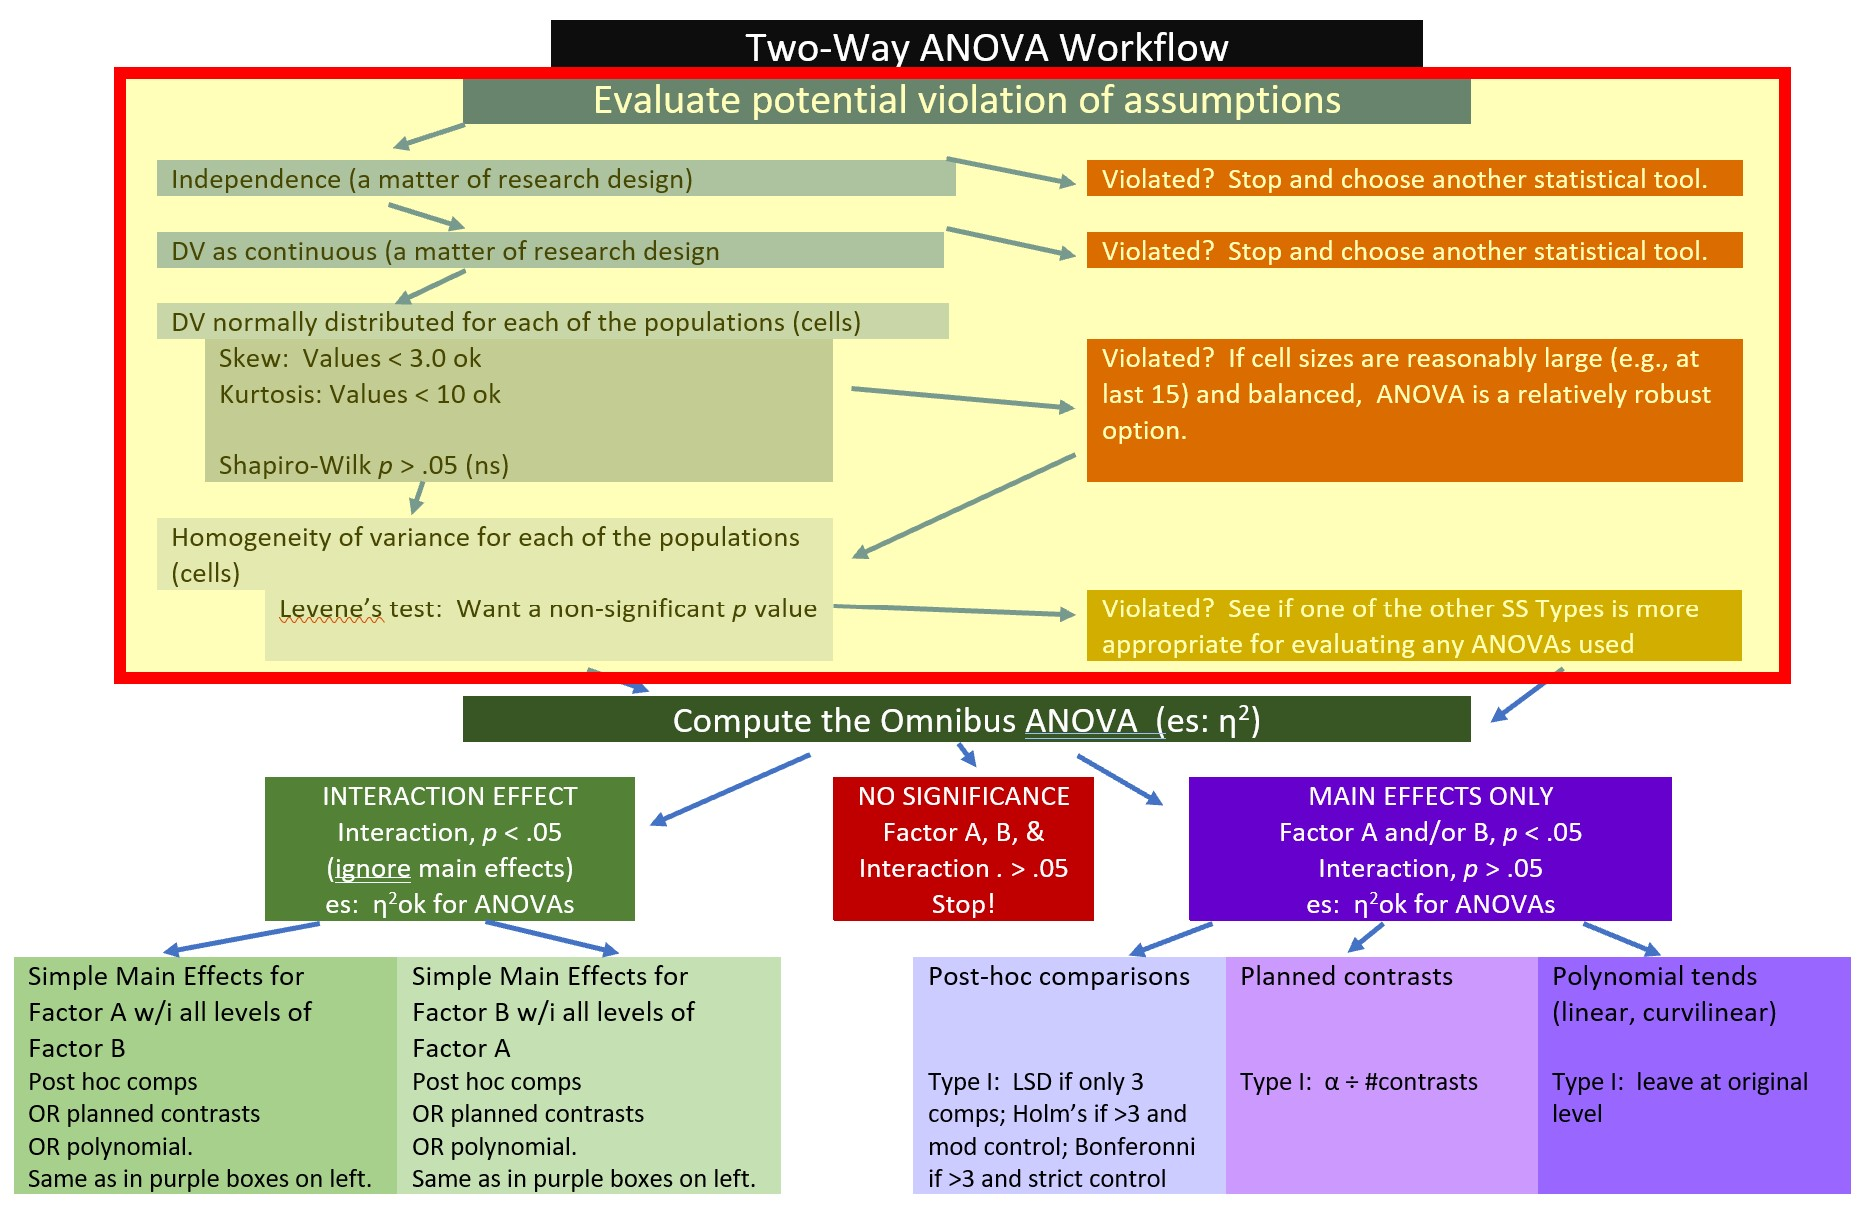
\includegraphics{images/factorial/WrkFlw_Assumptions.jpg}
\caption{Image of a flowchart showing that we are on the ``Evaluating assumptions'' portion of the workflow}
\end{figure}

\begin{Shaded}
\begin{Highlighting}[]
\NormalTok{TwoWay\_neg }\OtherTok{\textless{}{-}} \FunctionTok{aov}\NormalTok{(Negative }\SpecialCharTok{\textasciitilde{}}\NormalTok{ Rater }\SpecialCharTok{*}\NormalTok{ Photo, Ramdhani\_df)}
\FunctionTok{summary}\NormalTok{(TwoWay\_neg)}
\end{Highlighting}
\end{Shaded}

\begin{verbatim}
             Df Sum Sq Mean Sq F value    Pr(>F)    
Rater         2  12.21   6.103   8.077  0.000546 ***
Photo         1  14.62  14.619  19.346 0.0000262 ***
Rater:Photo   2   8.61   4.304   5.696  0.004480 ** 
Residuals   105  79.34   0.756                      
---
Signif. codes:  0 '***' 0.001 '**' 0.01 '*' 0.05 '.' 0.1 ' ' 1
\end{verbatim}

\begin{Shaded}
\begin{Highlighting}[]
\FunctionTok{model.tables}\NormalTok{(TwoWay\_neg, }\StringTok{"means"}\NormalTok{)}
\end{Highlighting}
\end{Shaded}

\begin{verbatim}
Tables of means
Grand mean
         
2.947369 

 Rater 
    Dayaknese Javanese Madurese
        2.492    3.007    3.299
rep    35.000   37.000   39.000

 Photo 
    Dayaknese Madurese
        2.575    3.301
rep    54.000   57.000

 Rater:Photo 
           Photo
Rater       Dayaknese Madurese
  Dayaknese  1.818     3.129  
  rep       17.000    18.000  
  Javanese   2.524     3.465  
  rep       18.000    19.000  
  Madurese   3.301     3.298  
  rep       19.000    20.000  
\end{verbatim}

\hypertarget{dv-is-normally-distributed}{%
\subsubsection{DV is normally distributed}\label{dv-is-normally-distributed}}

Let's start by analyzing \textbf{skew} and \textbf{kurtosis}.

\begin{Shaded}
\begin{Highlighting}[]
\NormalTok{psych}\SpecialCharTok{::}\FunctionTok{describeBy}\NormalTok{(Negative }\SpecialCharTok{\textasciitilde{}}\NormalTok{ Rater }\SpecialCharTok{+}\NormalTok{ Photo, }\AttributeTok{mat =} \ConstantTok{TRUE}\NormalTok{, }\AttributeTok{data =}\NormalTok{ Ramdhani\_df,}
    \AttributeTok{digits =} \DecValTok{3}\NormalTok{)}
\end{Highlighting}
\end{Shaded}

\begin{verbatim}
    item    group1    group2 vars  n  mean    sd median trimmed   mad   min
X11    1 Dayaknese Dayaknese    1 17 1.818 0.768  1.692   1.783 0.694 0.706
X12    2  Javanese Dayaknese    1 18 2.524 0.742  2.391   2.460 0.569 1.406
X13    3  Madurese Dayaknese    1 19 3.301 1.030  3.314   3.321 1.294 1.406
X14    4 Dayaknese  Madurese    1 18 3.129 0.156  3.160   3.136 0.104 2.732
X15    5  Javanese  Madurese    1 19 3.465 0.637  3.430   3.456 0.767 2.456
X16    6  Madurese  Madurese    1 20 3.297 1.332  2.958   3.254 1.615 1.211
      max range   skew kurtosis    se
X11 3.453 2.747  0.513   -0.881 0.186
X12 4.664 3.258  1.205    1.475 0.175
X13 4.854 3.448 -0.126   -1.267 0.236
X14 3.423 0.691 -0.623    0.481 0.037
X15 4.631 2.175 -0.010   -1.307 0.146
X16 5.641 4.430  0.215   -1.238 0.298
\end{verbatim}

Using guidelines from Kline \citeyearpar{kline_principles_2016} our values for skewness should fall below 3.0 (they do) and all values for kurtosis should fall below 8 to 20 (ours do).

In a factorial design, the Shapiro-Wilk test is applied to residuals from the model itself. Examination of those residuals can give us a good indication of normality.

First, we extract the residuals (i.e., that which is left-over/unexplained) from the model. We can examine their distribution with a plot.

\begin{Shaded}
\begin{Highlighting}[]
\CommentTok{\# creates object of residuals}
\NormalTok{resid\_neg }\OtherTok{\textless{}{-}} \FunctionTok{residuals}\NormalTok{(TwoWay\_neg)}
\FunctionTok{hist}\NormalTok{(resid\_neg)}
\end{Highlighting}
\end{Shaded}

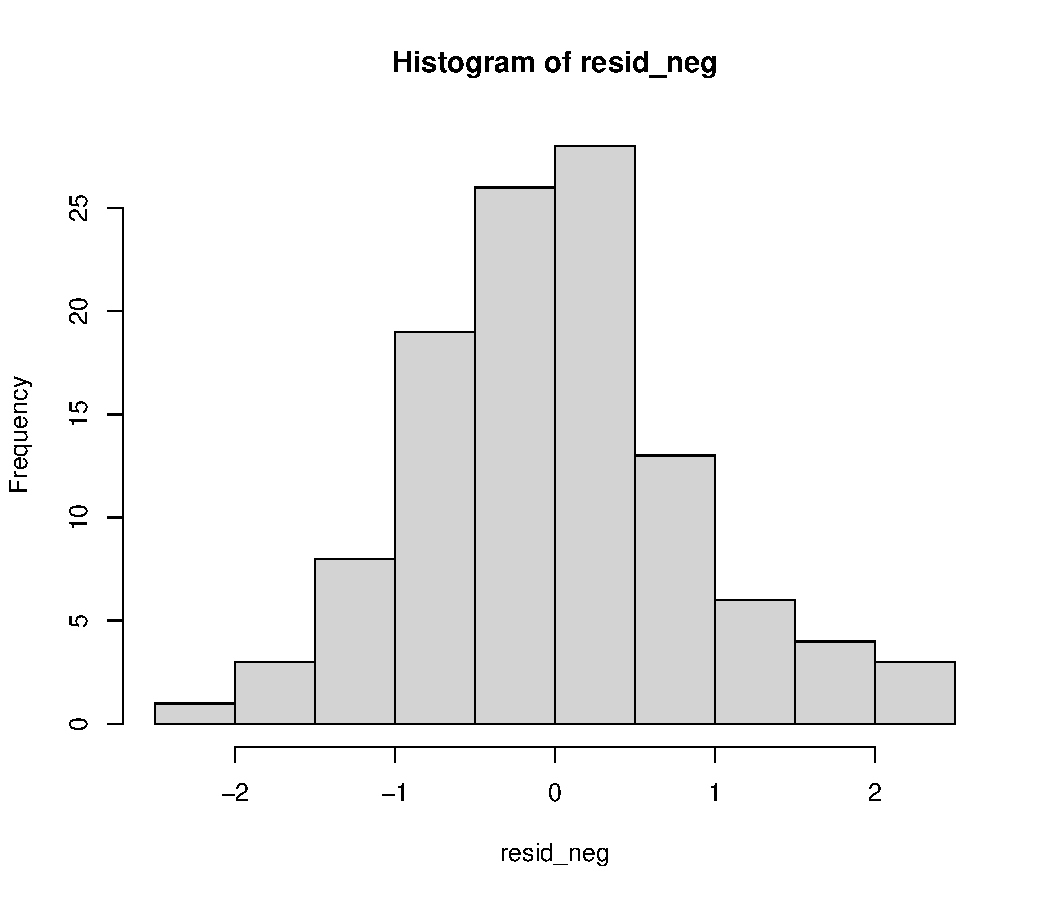
\includegraphics{ReCenterPsychStats_files/figure-latex/unnamed-chunk-140-1.pdf}
So far so good -- these look normal. Let's examine a QQ plot. We want the dots (the
Our distribution of \emph{residuals} (i.e., what is leftover after the model is applied) resembles a normal distribution.

The Q-Q plot provides another view. If the residuals are normally distributed, they will line up on the diagonal line (within reason).

\begin{Shaded}
\begin{Highlighting}[]
\FunctionTok{qqnorm}\NormalTok{(resid\_neg)}
\end{Highlighting}
\end{Shaded}

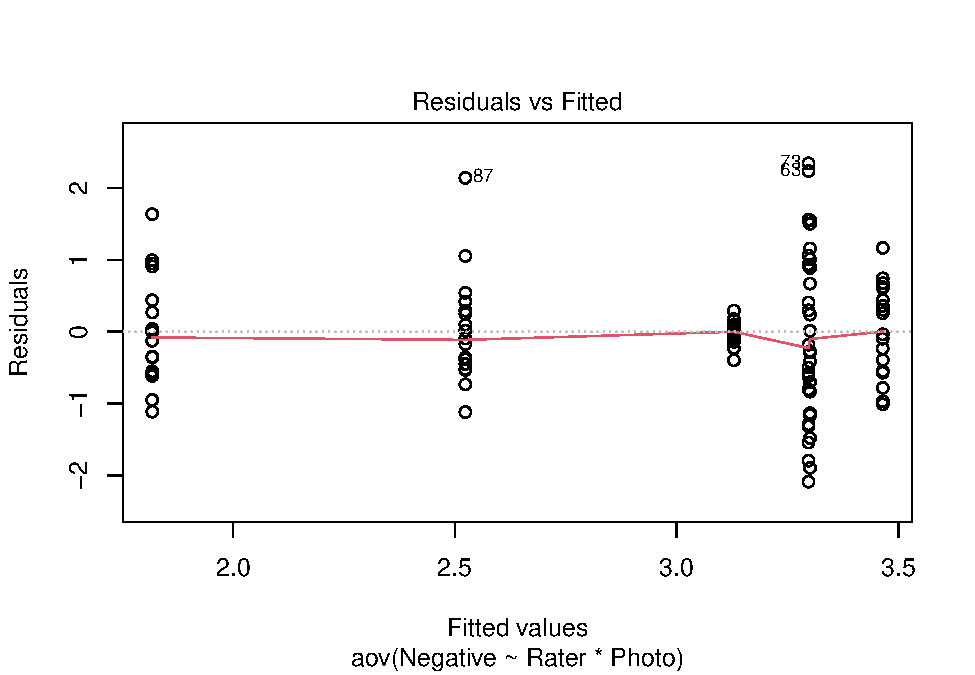
\includegraphics{ReCenterPsychStats_files/figure-latex/unnamed-chunk-141-1.pdf}
We can formally test the distribution of the residuals with a Shapiro test. We want the

We can formally test the distribution of the residuals with a Shapiro test. We want the associated \emph{p} value to be greather than 0.05.

\begin{Shaded}
\begin{Highlighting}[]
\FunctionTok{shapiro.test}\NormalTok{(resid\_neg)}
\end{Highlighting}
\end{Shaded}

\begin{verbatim}
    Shapiro-Wilk normality test

data:  resid_neg
W = 0.98464, p-value = 0.2344
\end{verbatim}

Whooo hoo! \(p > 0.05\)

Here's how I would summarize our data in terms of normality:

Factorial ANOVA assumes that the dependent variable is normally is distributed for all cells in the design. Our analysis suggested skew and kurtosis were within the bounds considered to be normally distributed. Further, the Shapiro-Wilk normality test (applied to the residuals from the factorial ANOVA model) suggested that the plotting of the residuals did not differ significantly from a normal distribution (\(W\) = 0.9846, \(p\) = 0.234).

\hypertarget{homogeneity-of-variance}{%
\subsubsection{Homogeneity of variance}\label{homogeneity-of-variance}}

We can evaluate the homogeneity of variance test with the Levene's test for the equality of error variances. Levene's requires a \emph{fully saturated model.} This means that the prediction model requires an interaction effect (not just two, non-interacting predictors). We can use the \emph{leveneTest()} function from the \emph{car} package. Within the function we specify the model we will be testing in the factorial ANOVA. That is, predicting Negative from the Rater and Photo factors. The asterisk indicates that they will also be added as an interaction term.

\begin{Shaded}
\begin{Highlighting}[]
\NormalTok{car}\SpecialCharTok{::}\FunctionTok{leveneTest}\NormalTok{(Negative }\SpecialCharTok{\textasciitilde{}}\NormalTok{ Rater }\SpecialCharTok{*}\NormalTok{ Photo, }\AttributeTok{data =}\NormalTok{ Ramdhani\_df)}
\end{Highlighting}
\end{Shaded}

\begin{verbatim}
Levene's Test for Homogeneity of Variance (center = median)
       Df F value       Pr(>F)    
group   5  8.6342 0.0000007002 ***
      105                         
---
Signif. codes:  0 '***' 0.001 '**' 0.01 '*' 0.05 '.' 0.1 ' ' 1
\end{verbatim}

Levene's test has indicated a violation of the homogeneity of variance assumption (\(F\){[}5, 105{]} = 8.634, \(p\) \textless{} .001). This is not surprising. The boxplots shows some widely varying variances.

\hypertarget{evaluating-the-omnibus-anova}{%
\subsection{Evaluating the Omnibus ANOVA}\label{evaluating-the-omnibus-anova}}

The \emph{F}-tests associated with the two-way ANOVA are the \emph{omnibus} -- providing the result for the main and interaction effects.

Here's where we are in the workflow.

\begin{figure}
\centering
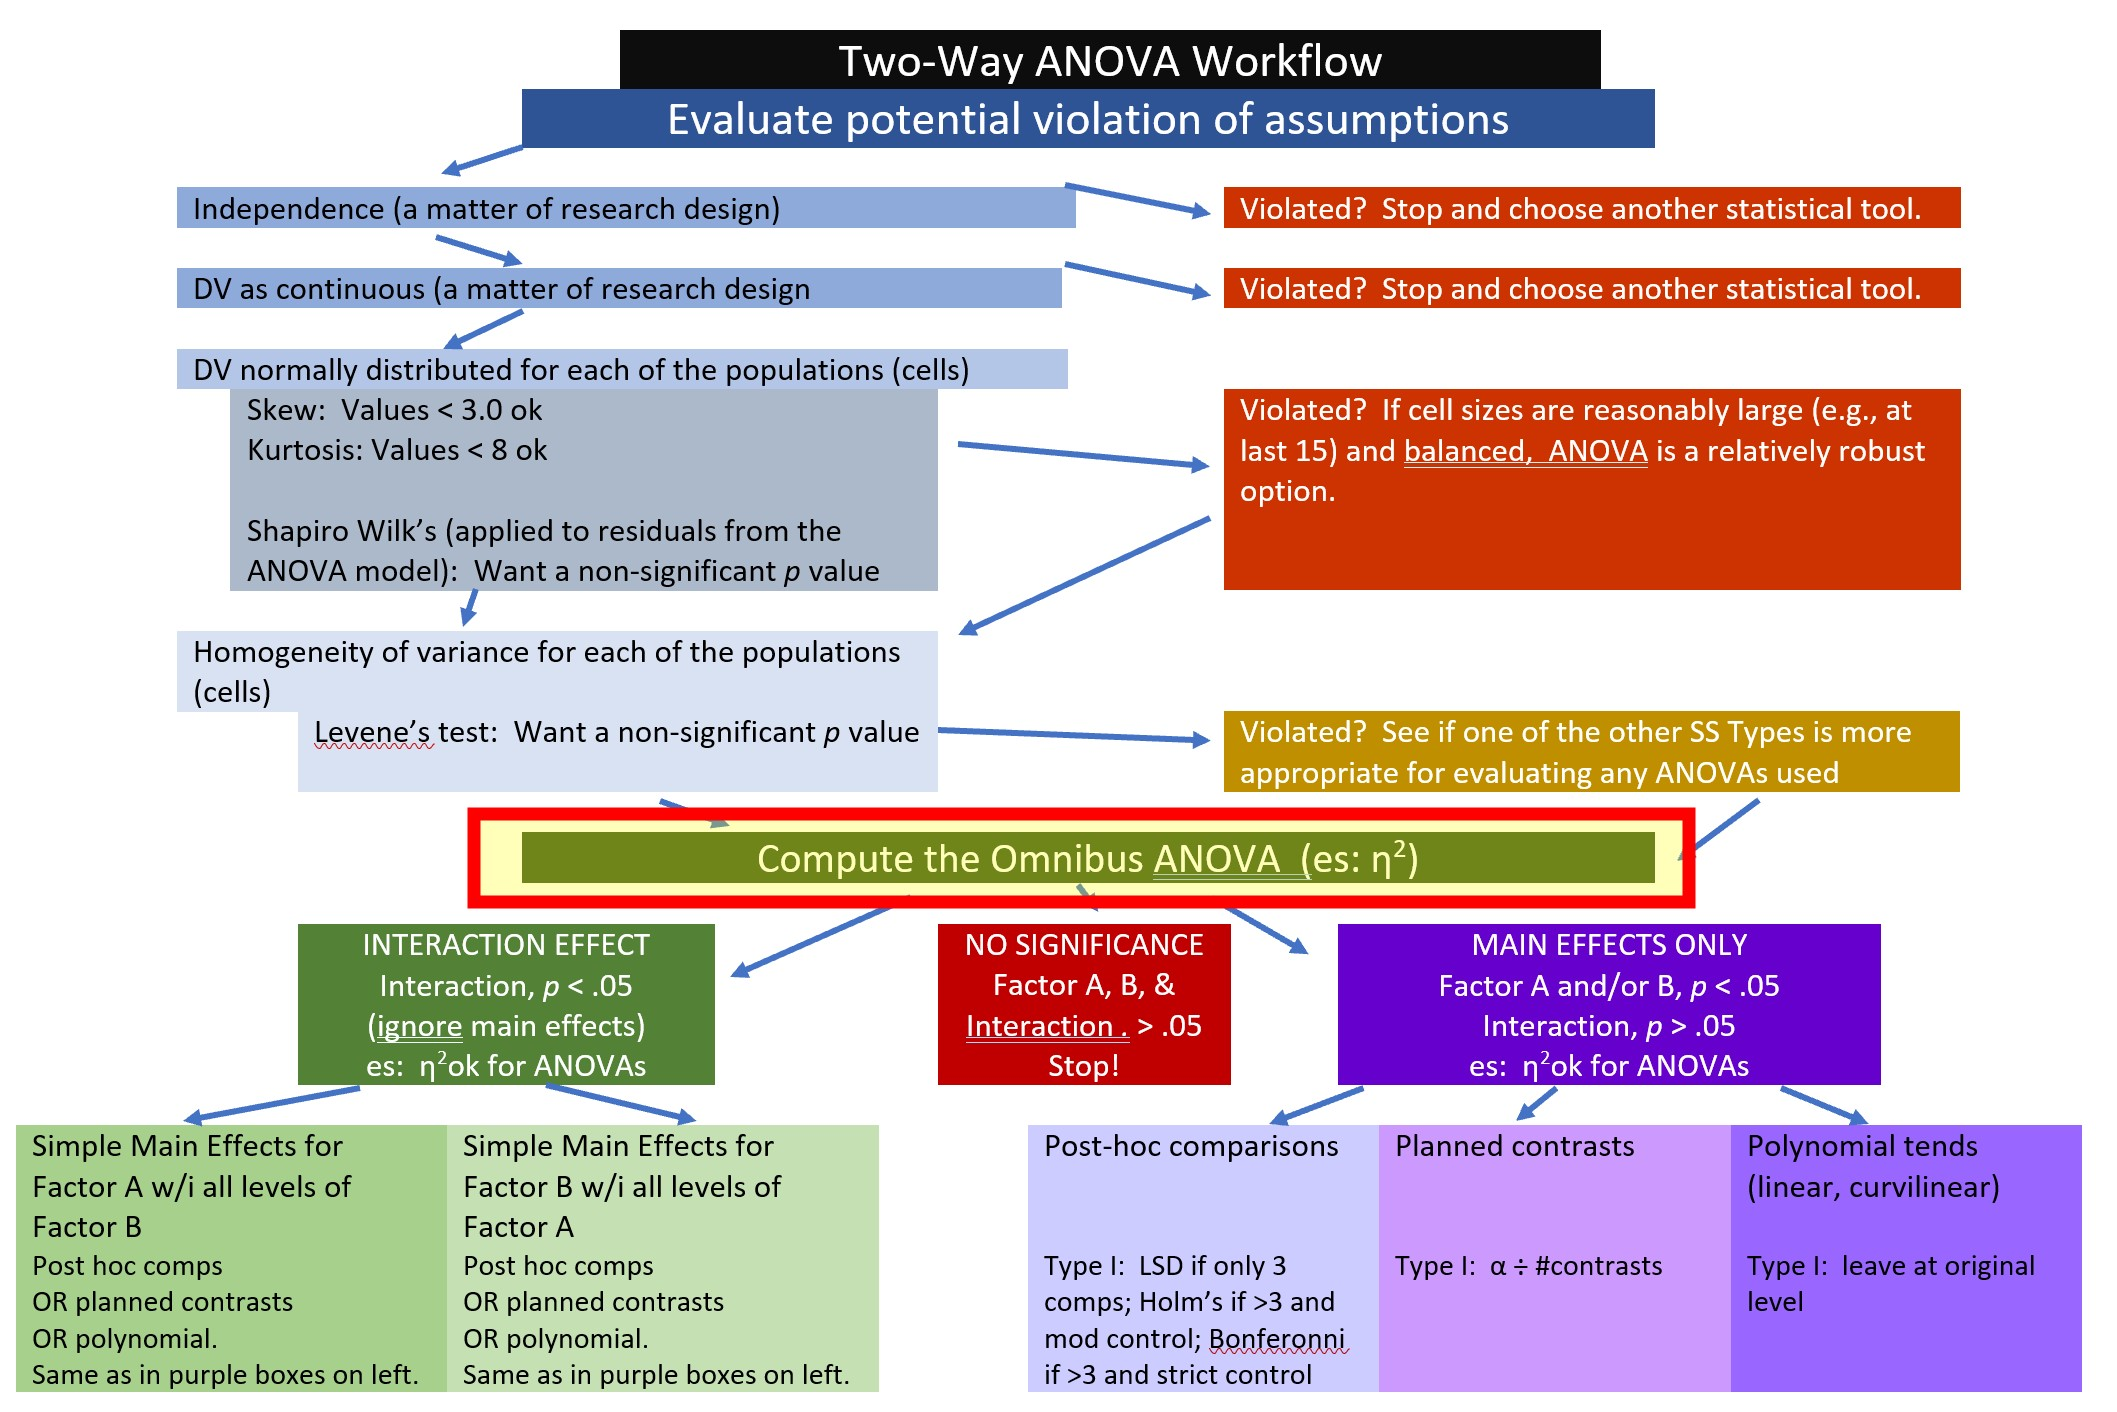
\includegraphics{images/factorial/WrkFlw_Omnibus.jpg}
\caption{Image our place in the Two-Way ANOVA Workflow.}
\end{figure}

When we run the two-way ANOVA we will be looking for several effects:

\begin{itemize}
\tightlist
\item
  main effects for each predictor, and
\item
  the interaction effect.
\end{itemize}

It is possible that all effects will be significant, none will be significant, or some will be significant. The interaction effect always takes precedence over the main effect because it let's us know there is a more nuanced/complex story.

In specifying the ANOVA, order of entry matters. If you have a distinction between IV and moderator, put the IV first.

\begin{Shaded}
\begin{Highlighting}[]
\NormalTok{TwoWay\_neg }\OtherTok{\textless{}{-}} \FunctionTok{aov}\NormalTok{(Negative }\SpecialCharTok{\textasciitilde{}}\NormalTok{ Rater }\SpecialCharTok{*}\NormalTok{ Photo, Ramdhani\_df)}
\FunctionTok{summary}\NormalTok{(TwoWay\_neg)}
\end{Highlighting}
\end{Shaded}

\begin{verbatim}
             Df Sum Sq Mean Sq F value    Pr(>F)    
Rater         2  12.21   6.103   8.077  0.000546 ***
Photo         1  14.62  14.619  19.346 0.0000262 ***
Rater:Photo   2   8.61   4.304   5.696  0.004480 ** 
Residuals   105  79.34   0.756                      
---
Signif. codes:  0 '***' 0.001 '**' 0.01 '*' 0.05 '.' 0.1 ' ' 1
\end{verbatim}

\begin{Shaded}
\begin{Highlighting}[]
\FunctionTok{model.tables}\NormalTok{(TwoWay\_neg, }\StringTok{"means"}\NormalTok{)}
\end{Highlighting}
\end{Shaded}

\begin{verbatim}
Tables of means
Grand mean
         
2.947369 

 Rater 
    Dayaknese Javanese Madurese
        2.492    3.007    3.299
rep    35.000   37.000   39.000

 Photo 
    Dayaknese Madurese
        2.575    3.301
rep    54.000   57.000

 Rater:Photo 
           Photo
Rater       Dayaknese Madurese
  Dayaknese  1.818     3.129  
  rep       17.000    18.000  
  Javanese   2.524     3.465  
  rep       18.000    19.000  
  Madurese   3.301     3.298  
  rep       19.000    20.000  
\end{verbatim}

Let's write the \emph{F strings}''* from the above table.

\begin{itemize}
\tightlist
\item
  Rater main effect: (\emph{F}{[}2, 105{]} = 8.077, \emph{p} \textless{} .001).
\item
  Photo stimulus main effect: (\emph{F}{[}1, 105{]} = 19.346, \emph{p} \textless{} .001).
\item
  Interaction effect: (\emph{F}{[}2, 105{]} = 5.696, \emph{p} = .004).
\end{itemize}

The \emph{plot()} function provides some quick plots from the object created from the ANOVA.

\begin{Shaded}
\begin{Highlighting}[]
\FunctionTok{plot}\NormalTok{(TwoWay\_neg)}
\end{Highlighting}
\end{Shaded}

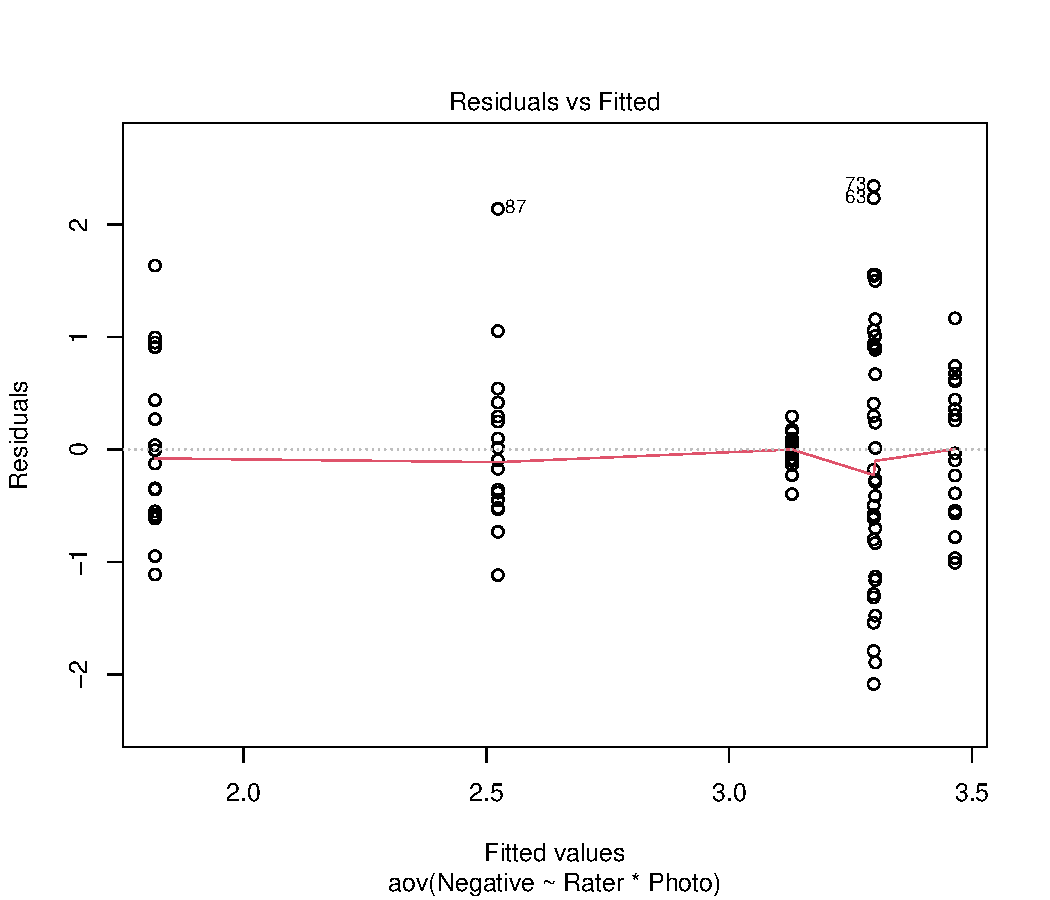
\includegraphics{ReCenterPsychStats_files/figure-latex/unnamed-chunk-145-1.pdf} 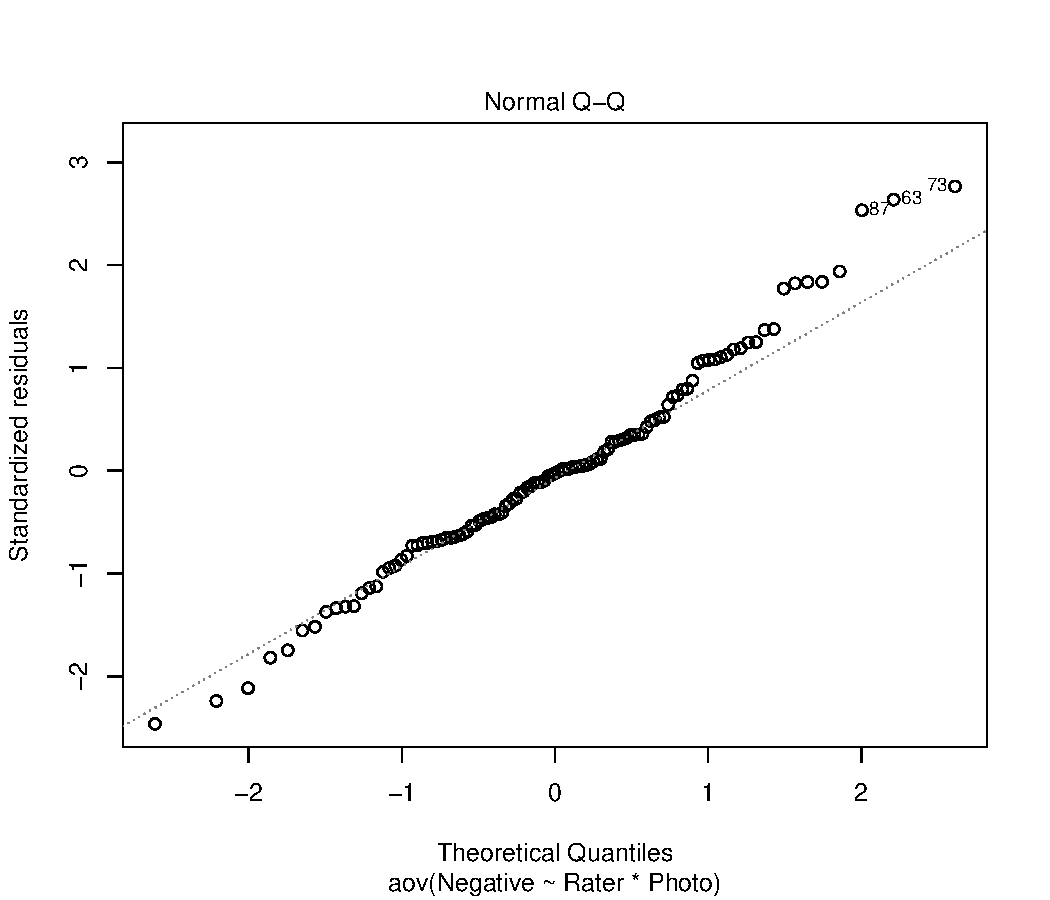
\includegraphics{ReCenterPsychStats_files/figure-latex/unnamed-chunk-145-2.pdf} 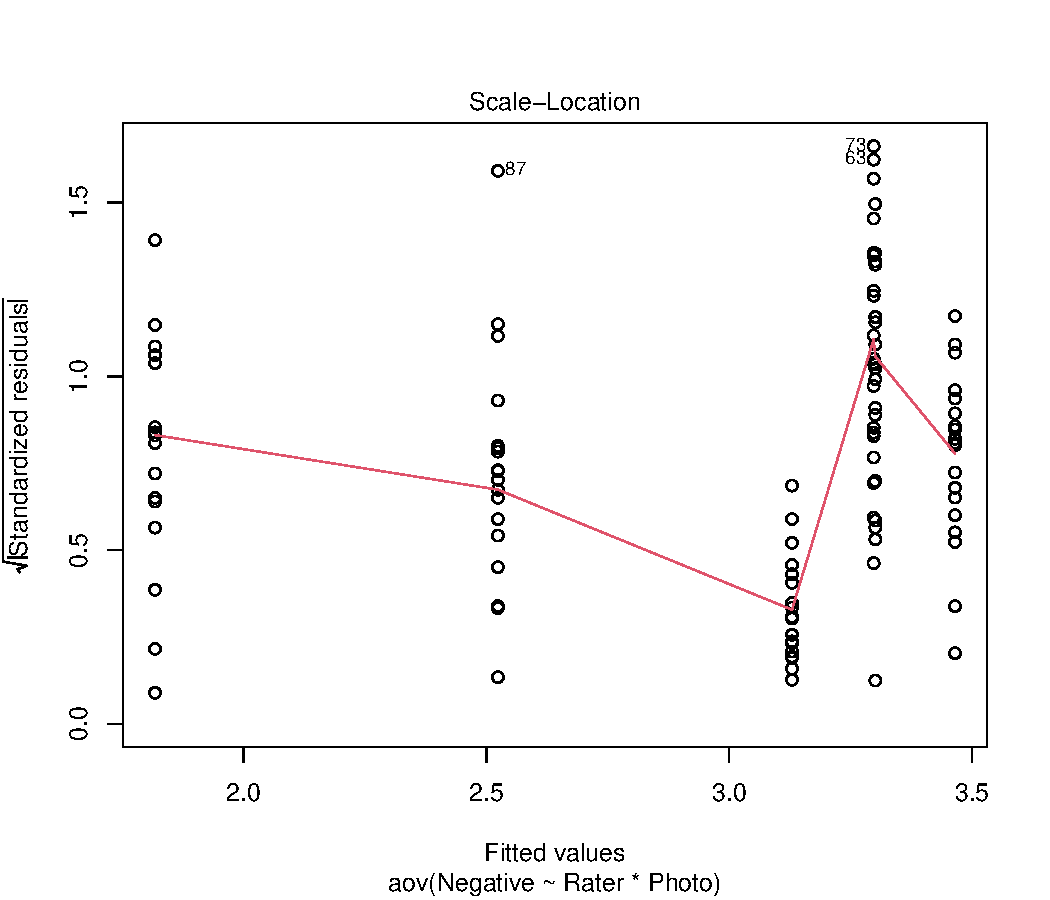
\includegraphics{ReCenterPsychStats_files/figure-latex/unnamed-chunk-145-3.pdf} 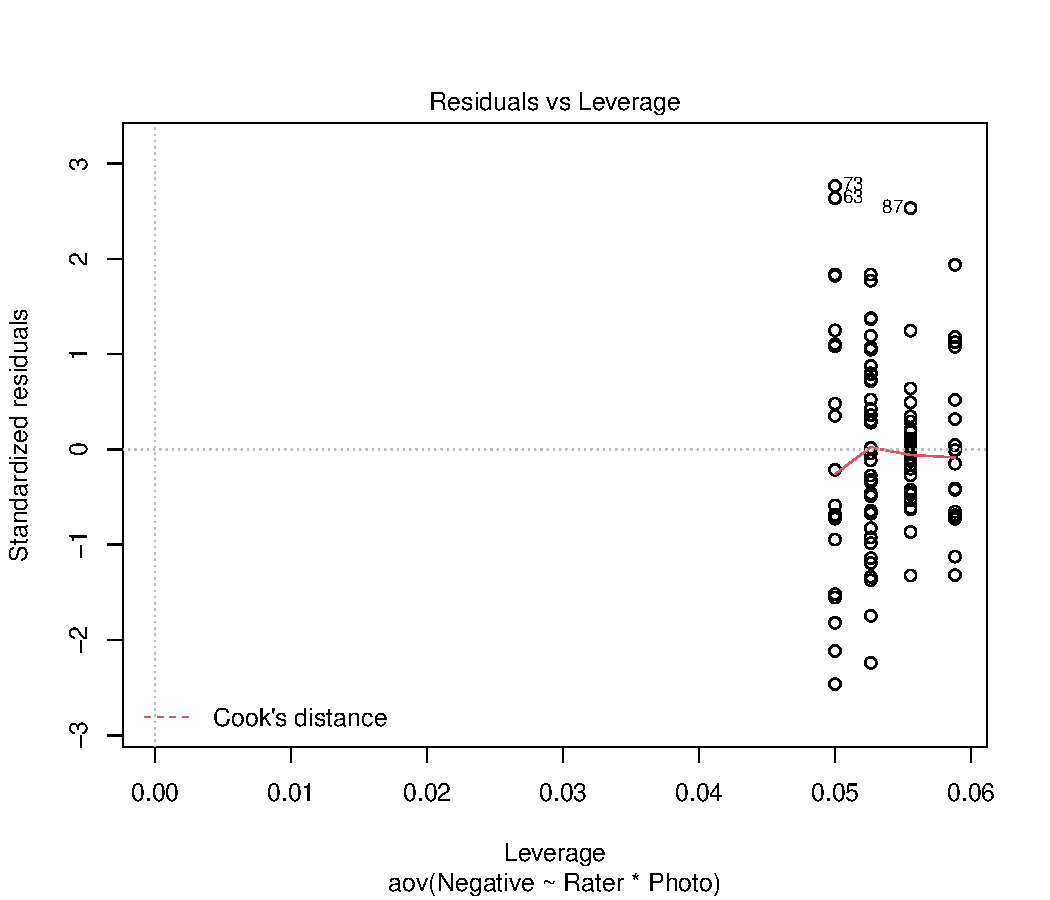
\includegraphics{ReCenterPsychStats_files/figure-latex/unnamed-chunk-145-4.pdf}

\hypertarget{effect-sizes}{%
\subsubsection{Effect sizes}\label{effect-sizes}}

\textbf{Eta squared} is one of the most commonly used measures of effect. It refers to the proportion of variability in the DV/outcome variable that can be explained in terms of the IVs/predictors. Traditional interpretive values are similar to the Pearson's \emph{r}:

\begin{itemize}
\tightlist
\item
  0 = no relationship
\item
  .02 = small
\item
  .13 = medium
\item
  .26 = large
\item
  1.0 = a perfect (one-to-one) correspondence
\end{itemize}

The formula for \(\eta ^{2}\) is straightforward:

\[\eta ^{2}=\frac{SS_{M}}{SS_{T}}\]
We can apply the \emph{etaSquared()} function from the \emph{lsr} package to our ANOVA object to retrieve \$\eta \^{}\{2\}.

\begin{Shaded}
\begin{Highlighting}[]
\NormalTok{lsr}\SpecialCharTok{::}\FunctionTok{etaSquared}\NormalTok{(TwoWay\_neg)}
\end{Highlighting}
\end{Shaded}

\begin{verbatim}
                eta.sq eta.sq.part
Rater       0.10662441  0.13363091
Photo       0.12736755  0.15558329
Rater:Photo 0.07500609  0.09788289
\end{verbatim}

We can update our \emph{F} strings to include the effect size:

\begin{itemize}
\tightlist
\item
  Rater main effect: (\emph{F}{[}2, 105{]} = 8.077, \emph{p} \textless{} .001, \(\eta ^{2}\) = 0.107).
\item
  Photo stimulus main effect: (\emph{F}{[}1, 105{]} = 19.346, \emph{p} \textless{} .001, \(\eta ^{2}\) = 0.127).
\item
  Interaction effect: (\emph{F}{[}2, 105{]} = 5.696, \emph{p} = .004, \(\eta ^{2}\) = 0.075).
\end{itemize}

Before moving to follow-up, let's capture an APA style write-up so far.

\hypertarget{apa-write-up-of-the-omnibus-results}{%
\subsubsection{APA Write-up of the omnibus results}\label{apa-write-up-of-the-omnibus-results}}

A 3 X 2 ANOVA was conducted to evaluate the effects of rater ethnicity (3 levels, Dayaknese, Madurese, Javanese) and photo stimulus (2 levels, Dayaknese on Madurese,) on negative reactions to the photo stimuli. Results of Levene's Test for Equality of Error Variances indicated violation of the homogeneity of variance assumption, (\(F\){[}5, 105{]} = 8.834, \(p\) \textless{} .001). Our analysis of the individual cell means (see Table 1 for means and standard deviations) suggested skew and kurtosis were within the bounds considered to be normally distributed \citep{kline_principles_2016}. A non-significant Shapiro-Wilk normality test (applied to the residuals from the factorial ANOVA model) provided further evidence that the assumption of normality was not violated (\(W\) = 0.9846, \(p\) = 0.234).

Computing sums of squares with a Type II approach, the results for the ANOVA indicated a significant main effect for ethnicity of the rater (\emph{F}{[}2, 105{]} = 8.077, \emph{p} \textless{} .001, \(\eta ^{2}\) = 0.107), a significant main effect for photo stimulus, (\emph{F}{[}1, 105{]} = 19.346, \emph{p} \textless{} .001, \(\eta ^{2}\) = 0.127), and a significant interaction effect (\emph{F}{[}2, 105{]} = 5.696, \emph{p} = .004, \(\eta ^{2}\) = 0.075).

\emph{Note. The next paragraph will have one of the follow-up options. We will add it later in the lesson}

\hypertarget{follow-up-a-significant-interaction-effect}{%
\subsection{Follow-up a significant interaction effect}\label{follow-up-a-significant-interaction-effect}}

In factorial ANOVA we are interested in main effects and interaction effects. When the result is explained by a main effect, then there is a consistent trend as a function of a factor (e.g., Madurese raters had consistently higher Negative evaluations, irrespective of stimulus). In an interaction effect, the results are more complex (e.g., the ratings across the stimulus differed for the three groups of raters).

There are a variety of strategies to follow-up a significant interaction effect. I will demonstrate the four I believe to be the most useful in the context of psychologists operating within the scientist-practitioner-advocacy context.

When an interaction effect is significant (irrespective of the significance of one or more main effects), examination of \textbf{simple main effects} is a common statistical/explanatory approached that is used. The Two-Way ANOVA Workflow shows where we are in this process.

\begin{figure}
\centering
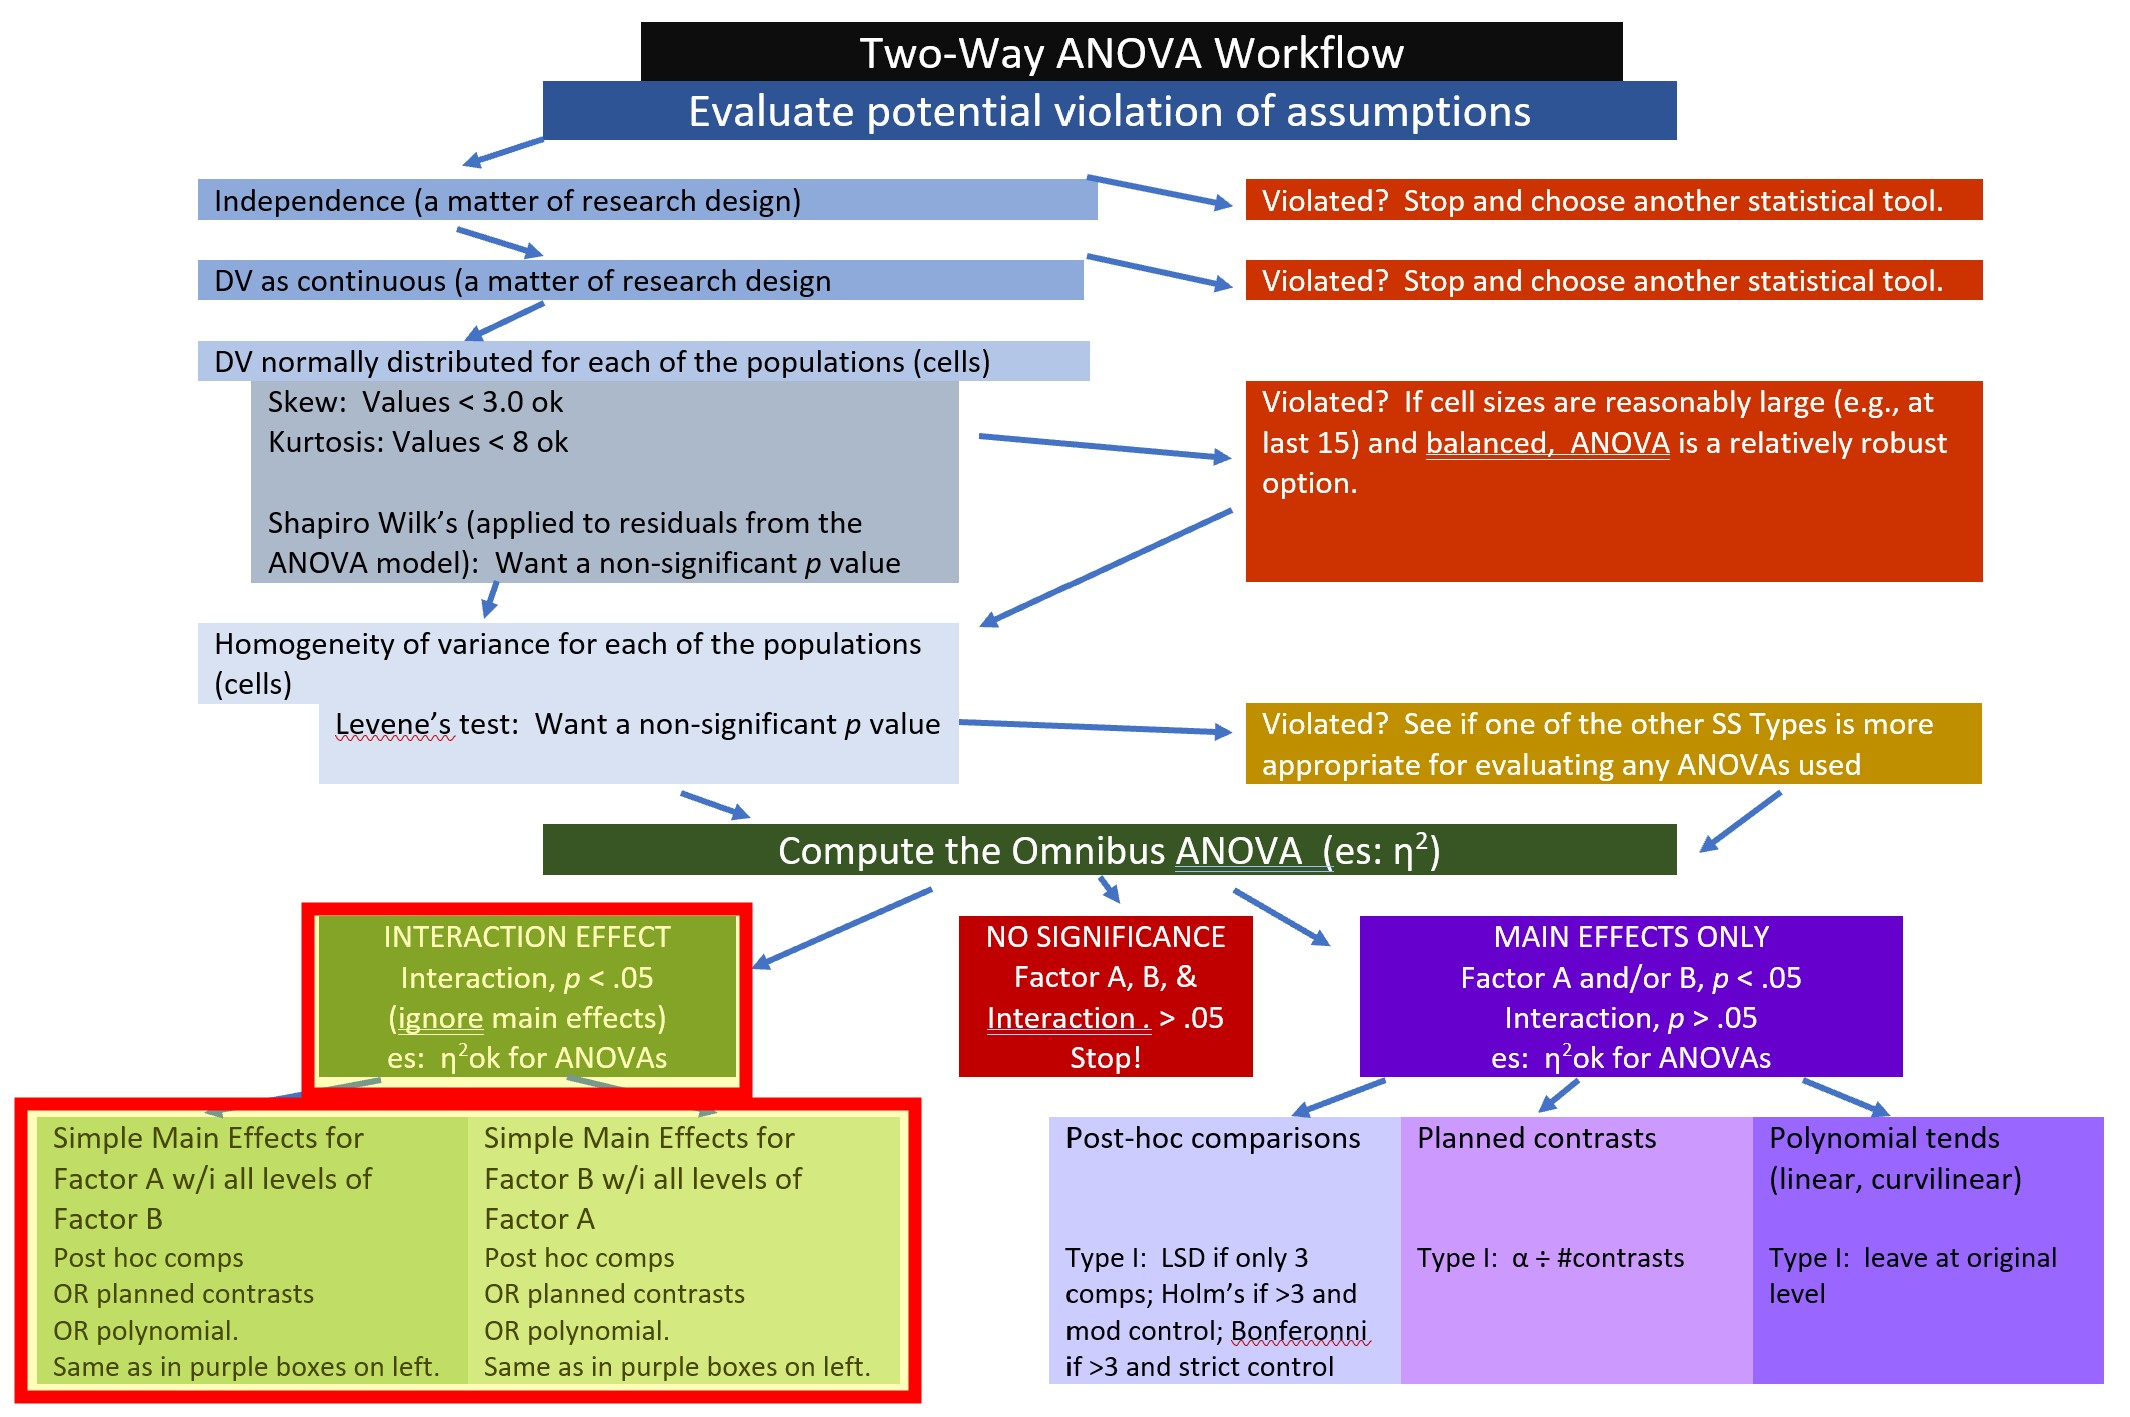
\includegraphics{images/factorial/WrkFlo_IntSmp.jpg}
\caption{Image our place in the Two-Way ANOVA Workflow.}
\end{figure}

\hypertarget{option-1-the-simple-main-effect-of-photo-stimulus-within-ethnicity-of-the-rater}{%
\subsubsection{Option \#1 the simple main effect of photo stimulus within ethnicity of the rater}\label{option-1-the-simple-main-effect-of-photo-stimulus-within-ethnicity-of-the-rater}}

Here we subset each of the three ethnic groups and then compare their ratings of the two photos. Essentially, we are conducting a one-way ANOVA for the Dyaknese ratings of the Dayaknese and Madurese photos.

\begin{Shaded}
\begin{Highlighting}[]
\CommentTok{\# subset data}
\NormalTok{Dayaknese }\OtherTok{\textless{}{-}} \FunctionTok{subset}\NormalTok{(Ramdhani\_df, Rater }\SpecialCharTok{==} \StringTok{"Dayaknese"}\NormalTok{)}
\CommentTok{\# change df to subset, new model name}
\NormalTok{Dayaknese\_simple }\OtherTok{\textless{}{-}} \FunctionTok{aov}\NormalTok{(Negative }\SpecialCharTok{\textasciitilde{}}\NormalTok{ Photo, }\AttributeTok{data =}\NormalTok{ Dayaknese)}
\CommentTok{\# output for simple main effect}
\FunctionTok{summary}\NormalTok{(Dayaknese\_simple)}
\end{Highlighting}
\end{Shaded}

\begin{verbatim}
            Df Sum Sq Mean Sq F value       Pr(>F)    
Photo        1 15.040  15.040    50.4 0.0000000395 ***
Residuals   33  9.847   0.298                         
---
Signif. codes:  0 '***' 0.001 '**' 0.01 '*' 0.05 '.' 0.1 ' ' 1
\end{verbatim}

\begin{Shaded}
\begin{Highlighting}[]
\CommentTok{\# effect size for simple main effect can add \textquotesingle{}type = 1,2,3,4\textquotesingle{} to}
\CommentTok{\# correspond with the ANOVA that was run}
\NormalTok{lsr}\SpecialCharTok{::}\FunctionTok{etaSquared}\NormalTok{(Dayaknese\_simple, }\AttributeTok{anova =} \ConstantTok{FALSE}\NormalTok{)}
\end{Highlighting}
\end{Shaded}

\begin{verbatim}
         eta.sq eta.sq.part
Photo 0.6043362   0.6043362
\end{verbatim}

Within the Dayaknese ethnic group, there is a statistically significant difference in negative reactions to Dayaknese and Madurese photos: \emph{F} (1, 33) = 50.4, \emph{p} \textless{} .001, \(\eta ^{2}\) = 0.60.

Next we evaluate photo rating within the Madurese ethnic group.

\begin{Shaded}
\begin{Highlighting}[]
\CommentTok{\# subset data}
\NormalTok{Madurese }\OtherTok{\textless{}{-}} \FunctionTok{subset}\NormalTok{(Ramdhani\_df, Rater }\SpecialCharTok{==} \StringTok{"Madurese"}\NormalTok{)}
\CommentTok{\# change df to subset, new model name}
\NormalTok{Madurese\_simple }\OtherTok{\textless{}{-}} \FunctionTok{aov}\NormalTok{(Negative }\SpecialCharTok{\textasciitilde{}}\NormalTok{ Photo, }\AttributeTok{data =}\NormalTok{ Madurese)}
\CommentTok{\# output for simple main effect}
\FunctionTok{summary}\NormalTok{(Madurese\_simple)}
\end{Highlighting}
\end{Shaded}

\begin{verbatim}
            Df Sum Sq Mean Sq F value Pr(>F)
Photo        1   0.00  0.0001       0  0.993
Residuals   37  52.82  1.4275               
\end{verbatim}

\begin{Shaded}
\begin{Highlighting}[]
\CommentTok{\# effect size for simple main effect can add \textquotesingle{}type = 1,2,3,4\textquotesingle{} to}
\CommentTok{\# correspond with the ANOVA that was run}
\NormalTok{lsr}\SpecialCharTok{::}\FunctionTok{etaSquared}\NormalTok{(Madurese\_simple, }\AttributeTok{anova =} \ConstantTok{FALSE}\NormalTok{)}
\end{Highlighting}
\end{Shaded}

\begin{verbatim}
              eta.sq    eta.sq.part
Photo 0.000002060568 0.000002060568
\end{verbatim}

Within the Madurese ethnic group, there was a nonsignificant difference in negative reactions to Dayaknese and Madurese photos: \emph{F} (1, 37) = 0.00, \emph{p} = .993, \(\eta ^{2}\) \textless{} .001.

\begin{Shaded}
\begin{Highlighting}[]
\CommentTok{\# subset data}
\NormalTok{Javanese }\OtherTok{\textless{}{-}} \FunctionTok{subset}\NormalTok{(Ramdhani\_df, Rater }\SpecialCharTok{==} \StringTok{"Javanese"}\NormalTok{)}
\CommentTok{\# change df to subset, new model name}
\NormalTok{Javanese\_simple }\OtherTok{\textless{}{-}} \FunctionTok{aov}\NormalTok{(Negative }\SpecialCharTok{\textasciitilde{}}\NormalTok{ Photo, }\AttributeTok{data =}\NormalTok{ Javanese)}
\CommentTok{\# output for simple main effect}
\FunctionTok{summary}\NormalTok{(Javanese\_simple)}
\end{Highlighting}
\end{Shaded}

\begin{verbatim}
            Df Sum Sq Mean Sq F value   Pr(>F)    
Photo        1  8.188   8.188   17.18 0.000205 ***
Residuals   35 16.678   0.477                     
---
Signif. codes:  0 '***' 0.001 '**' 0.01 '*' 0.05 '.' 0.1 ' ' 1
\end{verbatim}

\begin{Shaded}
\begin{Highlighting}[]
\CommentTok{\# effect size for simple main effect can add \textquotesingle{}type = 1,2,3,4\textquotesingle{} to}
\CommentTok{\# correspond with the ANOVA that was run}
\NormalTok{lsr}\SpecialCharTok{::}\FunctionTok{etaSquared}\NormalTok{(Javanese\_simple, }\AttributeTok{anova =} \ConstantTok{FALSE}\NormalTok{)}
\end{Highlighting}
\end{Shaded}

\begin{verbatim}
         eta.sq eta.sq.part
Photo 0.3292776   0.3292776
\end{verbatim}

Within the Javanese ethnic group, there was a significant difference in negative reactions to Dayaknese and Madurese photos: \emph{F} (1, 35) = 17.18, \emph{p} \textless{} .001, \(\eta ^{2}\) = 0.33.

If I were using this approach in a 3 X 2 ANOVA, I would probably not control for Type I error. Why? I only conducted follow-up comparisons to evaluate the simple main effect of photo stimulus within rater ethnicity; that is, I would hold it at alpha = 0.05.

\begin{itemize}
\tightlist
\item
  Photo stimulus (Dayaknese or Madurese) within the Dayaknese ethnic group.
\item
  Photo stimulus (Dayaknese or Madurese) within the Madurese ethnic group.
\item
  Photo stimulus (Dayaknese or Madurese) within the Javanese ethnic group.
\end{itemize}

However, because it is good for instruction, it would be equally fine to use a traditional Bonferroni, dividing .05/3 = 0.017 and testing each at 0.017. I will use this approach in the write-up.

FAQ: Could we do the reverse simple effect, ethnicity of rater within the photo stimulus? Absolutely! The choice is yours (and sometimes the results will differ). I usually run both and then report ONE -- the one that conveys the story the data has to tell. You \emph{could} report both sets, but then you would really want to control Type I error and your repetitive contrasts are far from independent/orthogonal.

\textbf{APA Style Results for Option \#1 follow-up.} \emph{This would be added to the results of the omnibus two-way ANOVA.}

\emph{Option \#1}: To explore the interaction effect, we followed with a test of the simple main effect of photo stimulus within the ethnicity of the rater. That is, we looked at the effect of the photo stimulus within the Dayaknese, Madurese, and Javanese groups, separately. To control for Type I error across the three simple main effects, we set alpha at .017 (.05/3). Results indicated significant differences for Dayaknese (\emph{F} {[}1, 33{]} = 50.4, \emph{p} \textless{} .001, \(\eta ^{2}\) = 0.60.) and Javanese ethnic groups (\emph{F} {[}1, 35{]}= 17.18, \emph{p} \textless{} .001, \(\eta ^{2}\) = 0.33), but not for the Madurese ethnic group (\emph{F} {[}1, 37{]} = 0.000, \emph{p} = .993, \(\eta ^{2}\) \textless{} .001). As illustrated in Figure 1, the Dayaknese and Javanese rathers both reported stronger negative reactions to the Madurese. The differences in ratings for the Madurese were not statistically significantly different. In this way, the rater's ethnic group moderated the relationship between the photo stimulus and negative reactions.

\begin{Shaded}
\begin{Highlighting}[]
\NormalTok{ggpubr}\SpecialCharTok{::}\FunctionTok{ggboxplot}\NormalTok{(Ramdhani\_df, }\AttributeTok{x =} \StringTok{"Rater"}\NormalTok{, }\AttributeTok{y =} \StringTok{"Negative"}\NormalTok{, }\AttributeTok{color =} \StringTok{"Photo"}\NormalTok{,}
    \AttributeTok{xlab =} \StringTok{"Ethnicity of Rater"}\NormalTok{, }\AttributeTok{ylab =} \StringTok{"Negative Reaction"}\NormalTok{)}
\end{Highlighting}
\end{Shaded}

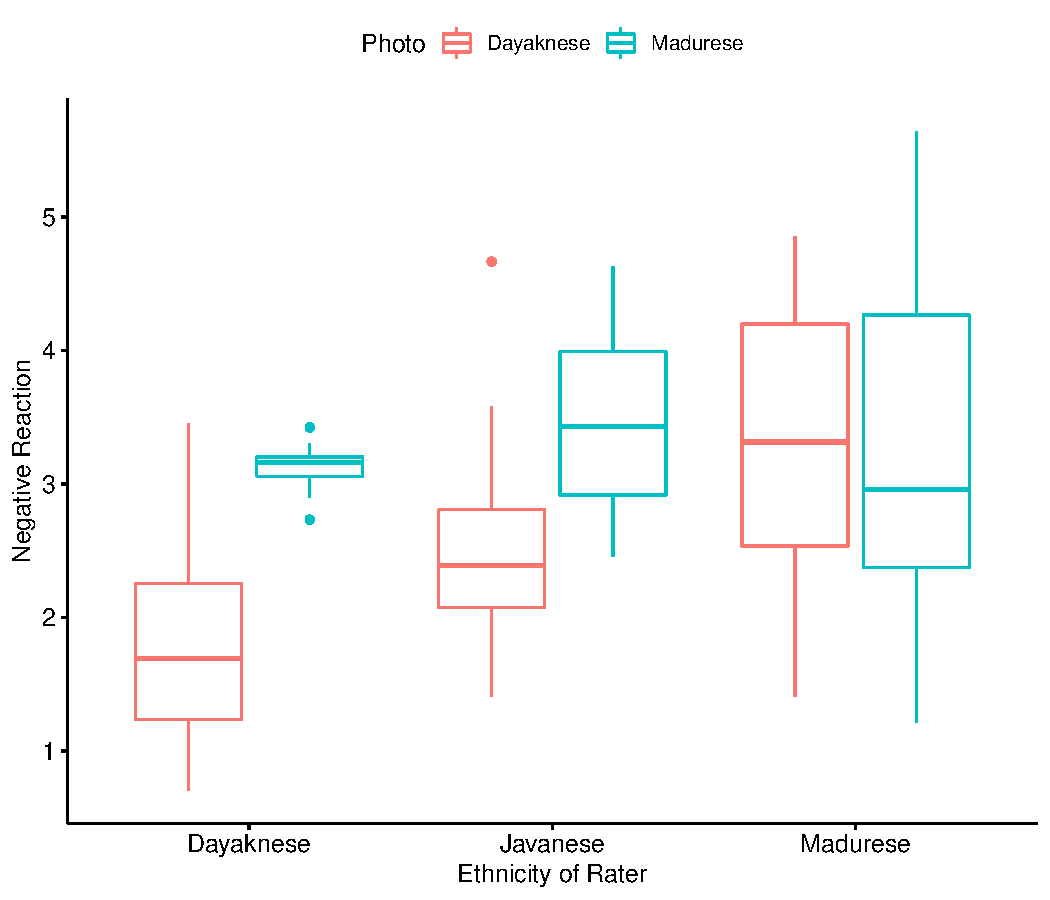
\includegraphics{ReCenterPsychStats_files/figure-latex/unnamed-chunk-150-1.pdf}

\hypertarget{option-2-the-simple-main-effect-of-ethnicity-of-rater-within-photo-stimulus.}{%
\subsubsection{Option \#2 the simple main effect of ethnicity of rater within photo stimulus.}\label{option-2-the-simple-main-effect-of-ethnicity-of-rater-within-photo-stimulus.}}

In this simple main effect of ethnicity of rater (3 levels) within photo stimulus (2 levels), we will conduct two one-way ANOVAs for the Dayaknese and Madurese photos, separately. However, we will want to do orthogonal contrast-coding for rater ethnicity for the follow-up (to the follow-up).

It helps to know what the default contrast codes are; we can get that information with the \emph{contrasts()} function.

\begin{Shaded}
\begin{Highlighting}[]
\FunctionTok{contrasts}\NormalTok{(Ramdhani\_df}\SpecialCharTok{$}\NormalTok{Rater)}
\end{Highlighting}
\end{Shaded}

\begin{verbatim}
          Javanese Madurese
Dayaknese        0        0
Javanese         1        0
Madurese         0        1
\end{verbatim}

Let's create custom contrasts. Recall that an orthogonal contrast requires that there be one less contrast than the number of groups and that once a group is singled out, it cannot be compared again.

Thus, I want to compare the

\begin{itemize}
\tightlist
\item
  Javanese to the Dayaknese and Madurese combined, then
\item
  Dayaknese to Madurese
\end{itemize}

\begin{Shaded}
\begin{Highlighting}[]
\CommentTok{\# tell R which groups to compare}
\NormalTok{c1 }\OtherTok{\textless{}{-}} \FunctionTok{c}\NormalTok{(}\DecValTok{1}\NormalTok{, }\SpecialCharTok{{-}}\DecValTok{2}\NormalTok{, }\DecValTok{1}\NormalTok{)}
\NormalTok{c2 }\OtherTok{\textless{}{-}} \FunctionTok{c}\NormalTok{(}\SpecialCharTok{{-}}\DecValTok{1}\NormalTok{, }\DecValTok{0}\NormalTok{, }\DecValTok{1}\NormalTok{)}
\NormalTok{mat }\OtherTok{\textless{}{-}} \FunctionTok{cbind}\NormalTok{(c1, c2)  }\CommentTok{\#combine the above bits}
\FunctionTok{contrasts}\NormalTok{(Ramdhani\_df}\SpecialCharTok{$}\NormalTok{Rater) }\OtherTok{\textless{}{-}}\NormalTok{ mat  }\CommentTok{\# attach the contrasts to the variable}
\end{Highlighting}
\end{Shaded}

This allows us to recheck the contrasts.

\begin{Shaded}
\begin{Highlighting}[]
\FunctionTok{contrasts}\NormalTok{(Ramdhani\_df}\SpecialCharTok{$}\NormalTok{Rater)}
\end{Highlighting}
\end{Shaded}

\begin{verbatim}
          c1 c2
Dayaknese  1 -1
Javanese  -2  0
Madurese   1  1
\end{verbatim}

Yes, in contrast 1 we are comparing the Javanese to the combined Dayaknese and Madurese. In contrast 2 we are comparing the Dayaknese to the Madureses.

\begin{Shaded}
\begin{Highlighting}[]
\CommentTok{\# subset data}
\NormalTok{Dayaknese\_Ph }\OtherTok{\textless{}{-}} \FunctionTok{subset}\NormalTok{(Ramdhani\_df, Photo }\SpecialCharTok{==} \StringTok{"Dayaknese"}\NormalTok{)}
\CommentTok{\# change df to subset, new model name}
\NormalTok{Dykn\_simple }\OtherTok{\textless{}{-}} \FunctionTok{aov}\NormalTok{(Negative }\SpecialCharTok{\textasciitilde{}}\NormalTok{ Rater, }\AttributeTok{data =}\NormalTok{ Dayaknese\_Ph)}
\CommentTok{\# output for simple main effect}
\FunctionTok{summary}\NormalTok{(Dykn\_simple)}
\end{Highlighting}
\end{Shaded}

\begin{verbatim}
            Df Sum Sq Mean Sq F value    Pr(>F)    
Rater        2  19.81   9.903   13.32 0.0000221 ***
Residuals   51  37.90   0.743                      
---
Signif. codes:  0 '***' 0.001 '**' 0.01 '*' 0.05 '.' 0.1 ' ' 1
\end{verbatim}

\begin{Shaded}
\begin{Highlighting}[]
\CommentTok{\# effect size for simple main effect can add \textquotesingle{}type = 1,2,3,4\textquotesingle{} to}
\CommentTok{\# correspond with the ANOVA that was run}
\NormalTok{lsr}\SpecialCharTok{::}\FunctionTok{etaSquared}\NormalTok{(Dykn\_simple, }\AttributeTok{anova =} \ConstantTok{FALSE}\NormalTok{)}
\end{Highlighting}
\end{Shaded}

\begin{verbatim}
         eta.sq eta.sq.part
Rater 0.3432006   0.3432006
\end{verbatim}

We can capture the \emph{F} string from this output: \emph{F} {[}2, 51{]}) = 13.32, \emph{p} \textless{} .001, \(\eta ^{2}\) = 0.343.

This code produces the contrasts we specified. Note that in our code we can improve the interpretability of the output by adding labels. We know the specific contrasts from our prior work.

\begin{Shaded}
\begin{Highlighting}[]
\FunctionTok{summary.aov}\NormalTok{(Dykn\_simple, }\AttributeTok{split =} \FunctionTok{list}\NormalTok{(}\AttributeTok{Rater =} \FunctionTok{list}\NormalTok{(}\StringTok{\textasciigrave{}}\AttributeTok{Javanese v Dayaknese and Madurese}\StringTok{\textasciigrave{}} \OtherTok{=} \DecValTok{1}\NormalTok{,}
    \StringTok{\textasciigrave{}}\AttributeTok{Dayaknese Madurese}\StringTok{\textasciigrave{}} \OtherTok{=} \DecValTok{2}\NormalTok{)))}
\end{Highlighting}
\end{Shaded}

\begin{verbatim}
                                           Df Sum Sq Mean Sq F value     Pr(>F)
Rater                                       2  19.81   9.903  13.325 0.00002211
  Rater: Javanese v Dayaknese and Madurese  1   0.07   0.071   0.095      0.759
  Rater: Dayaknese Madurese                 1  19.73  19.735  26.554 0.00000419
Residuals                                  51  37.90   0.743                   
                                              
Rater                                      ***
  Rater: Javanese v Dayaknese and Madurese    
  Rater: Dayaknese Madurese                ***
Residuals                                     
---
Signif. codes:  0 '***' 0.001 '**' 0.01 '*' 0.05 '.' 0.1 ' ' 1
\end{verbatim}

The simple main effect of ethnicity of the rater within the reaction to the photos of members of the Dayaknese ethnic group was statistically significant: \emph{F} {[}2, 51{]} = 13.32, \emph{p} \textless{} .001, \(\eta ^{2}\) = 0.343. Follow-up testing indicated non-significant differences when the ratings from members of the Javanese ethnic group were compared to the Dayaknese and Madurese, combined (\emph{F} {[}1, 51{]} = 0.095, \emph{p} = .759). There was a statistically significant difference when Dayaknese and Madurese raters were compared (\emph{F} {[}1, 51{]} =26.554, \emph{p} \textless{} .001)

We repeat the simple main effect process when the Madurese photos were the stimulus.

\begin{Shaded}
\begin{Highlighting}[]
\CommentTok{\# subset data}
\NormalTok{Madurese\_Ph }\OtherTok{\textless{}{-}} \FunctionTok{subset}\NormalTok{(Ramdhani\_df, Photo }\SpecialCharTok{==} \StringTok{"Madurese"}\NormalTok{)}
\CommentTok{\# change df to subset, new model name}
\NormalTok{Mdrs\_simple }\OtherTok{\textless{}{-}} \FunctionTok{aov}\NormalTok{(Negative }\SpecialCharTok{\textasciitilde{}}\NormalTok{ Rater, }\AttributeTok{data =}\NormalTok{ Madurese\_Ph)}
\CommentTok{\# output for simple main effect}
\FunctionTok{summary}\NormalTok{(Mdrs\_simple)}
\end{Highlighting}
\end{Shaded}

\begin{verbatim}
            Df Sum Sq Mean Sq F value Pr(>F)
Rater        2   1.04  0.5207   0.679  0.512
Residuals   54  41.44  0.7674               
\end{verbatim}

\begin{Shaded}
\begin{Highlighting}[]
\CommentTok{\# effect size for simple main effect can add \textquotesingle{}type = 1,2,3,4\textquotesingle{} to}
\CommentTok{\# correspond with the ANOVA that was run}
\NormalTok{lsr}\SpecialCharTok{::}\FunctionTok{etaSquared}\NormalTok{(Mdrs\_simple, }\AttributeTok{anova =} \ConstantTok{FALSE}\NormalTok{)}
\end{Highlighting}
\end{Shaded}

\begin{verbatim}
          eta.sq eta.sq.part
Rater 0.02451385  0.02451385
\end{verbatim}

Let's capture the \emph{F} string for ratings of the Madurese photos: \emph{F} {[}2, 54{]} = 0.679, \emph{p} = .512, \(\eta ^{2}\) = 0.024.

We can use the procedure described above to obtain our orthogonal contrasts.

\begin{Shaded}
\begin{Highlighting}[]
\FunctionTok{summary.aov}\NormalTok{(Mdrs\_simple, }\AttributeTok{split =} \FunctionTok{list}\NormalTok{(}\AttributeTok{Rater =} \FunctionTok{list}\NormalTok{(}\StringTok{\textasciigrave{}}\AttributeTok{Javanese v Dayaknese and Madurese}\StringTok{\textasciigrave{}} \OtherTok{=} \DecValTok{1}\NormalTok{,}
    \StringTok{\textasciigrave{}}\AttributeTok{Dayaknese Madurese}\StringTok{\textasciigrave{}} \OtherTok{=} \DecValTok{2}\NormalTok{)))}
\end{Highlighting}
\end{Shaded}

\begin{verbatim}
                                           Df Sum Sq Mean Sq F value Pr(>F)
Rater                                       2   1.04  0.5207   0.679  0.512
  Rater: Javanese v Dayaknese and Madurese  1   0.77  0.7734   1.008  0.320
  Rater: Dayaknese Madurese                 1   0.27  0.2679   0.349  0.557
Residuals                                  54  41.44  0.7674               
\end{verbatim}

Here's a write-up of this portion of the result.

The simple main effect of ethnicity of the rater within rating the photos of Madurese people was not statistically significant: (\emph{F} {[}2, 54{]} = 0.679, \emph{p} = .512, \(\eta ^{2}\) = 0.024). Correspondingly, follow-up testing indicated non-significant differences when the ratings of the Javanese were compared to Dayaknese and Madurese, combined (\emph{F} {[}1, 54{]} = 1.008, \emph{p} = .320) and when the ratings of the Dayaknese and Madurese were compared (\emph{F} {[}1, 54{]} = 0.349, \emph{p} = .557)

To control for Type I error, we have 4 follow-up contrasts (2 for Dayaknese, 2 for Madurese). We'll control Type I error with .05/4 = .0125

\begin{Shaded}
\begin{Highlighting}[]
\FloatTok{0.05}\SpecialCharTok{/}\DecValTok{4}
\end{Highlighting}
\end{Shaded}

\begin{verbatim}
[1] 0.0125
\end{verbatim}

\textbf{APA Write-up of the simple main effect of photo stimulus within rater ethnicity.}

This would be added to the write-up of the omnibus two-way ANOVA test.

\emph{Option \#2}: To explore the interaction effect, we followed with tests of simple effect of rater ethnicity within the photo stimulus. That is, we looked at the effect of each each rater's ethnicity within the Madurese and Dayaknese photo stimulus, separately. Our first analysis evaluated the effect of the rater's ethnicity when evaluating the Dayaknese photo; our second analysis evaluated effect of the rater's ethnicity when evaluating the Madurese photo. To control for Type I error across the two simple main effects, we set alpha at .0125 (.05/4). The simple main effect of ethnicity of the rater within the reaction to the photos of members of the Dayaknese ethnic group was statistically significant: \emph{F} {[}2, 51{]} = 13.32, \emph{p} \textless{} .001, \(\eta ^{2}\) = 0.343. Follow-up testing indicated non-significant differences when the ratings from members of the Javanese ethnic group were compared to the Dayaknese and Madurese, combined (\emph{F} {[}1, 51{]} = 0.095, \emph{p} = .759). There was a statistically significant difference when Dayaknese and Madurese raters were compared (\emph{F} {[}1, 51{]} =26.554, \emph{p} \textless{} .001). The simple main effect of ethnicity of the rater within when rating the photos of Madurese people was not statistically significant: (\emph{F} {[}2, 54{]} = 0.679, \emph{p} = .512, \(\eta ^{2}\) = 0.024). Correspondingly, follow-up testing indicated non-significant differences when the ratings of the Javanese were compared to Dayaknese and Madurese, combined (\emph{F} {[}1, 54{]} = 1.008, \emph{p} = .320) and when the ratings of the Dayaknese and Madurese were compared (\emph{F} {[}1, 54{]} = 0.349, \emph{p} = .557). This moderating effect of ethnicity of the rater on the negative reaction to the photo stimulus is illustrated in Figure 1.

\begin{Shaded}
\begin{Highlighting}[]
\NormalTok{ggpubr}\SpecialCharTok{::}\FunctionTok{ggboxplot}\NormalTok{(Ramdhani\_df, }\AttributeTok{x =} \StringTok{"Photo"}\NormalTok{, }\AttributeTok{y =} \StringTok{"Negative"}\NormalTok{, }\AttributeTok{color =} \StringTok{"Rater"}\NormalTok{,}
    \AttributeTok{xlab =} \StringTok{"Photo Stimulus"}\NormalTok{, }\AttributeTok{ylab =} \StringTok{"Negative Reaction"}\NormalTok{)}
\end{Highlighting}
\end{Shaded}

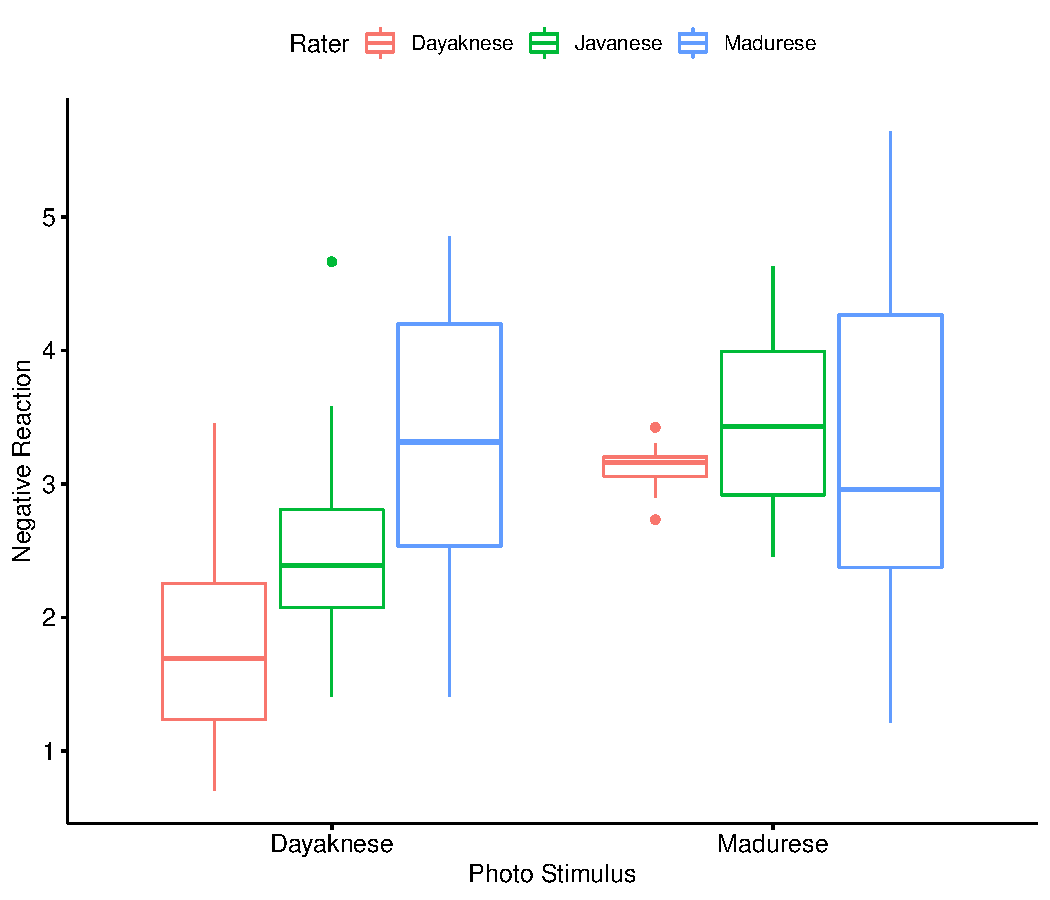
\includegraphics{ReCenterPsychStats_files/figure-latex/unnamed-chunk-159-1.pdf}

\hypertarget{option-3-post-hoc-comparisons}{%
\subsubsection{Option \#3 post hoc comparisons}\label{option-3-post-hoc-comparisons}}

Another option is compare all possible cells. These are termed \emph{post hoc comparisons.} They are an alternative to simple main effects; you would not report both. The figure shows our place on the Two-Way ANOVA Workflow.

\begin{figure}
\centering
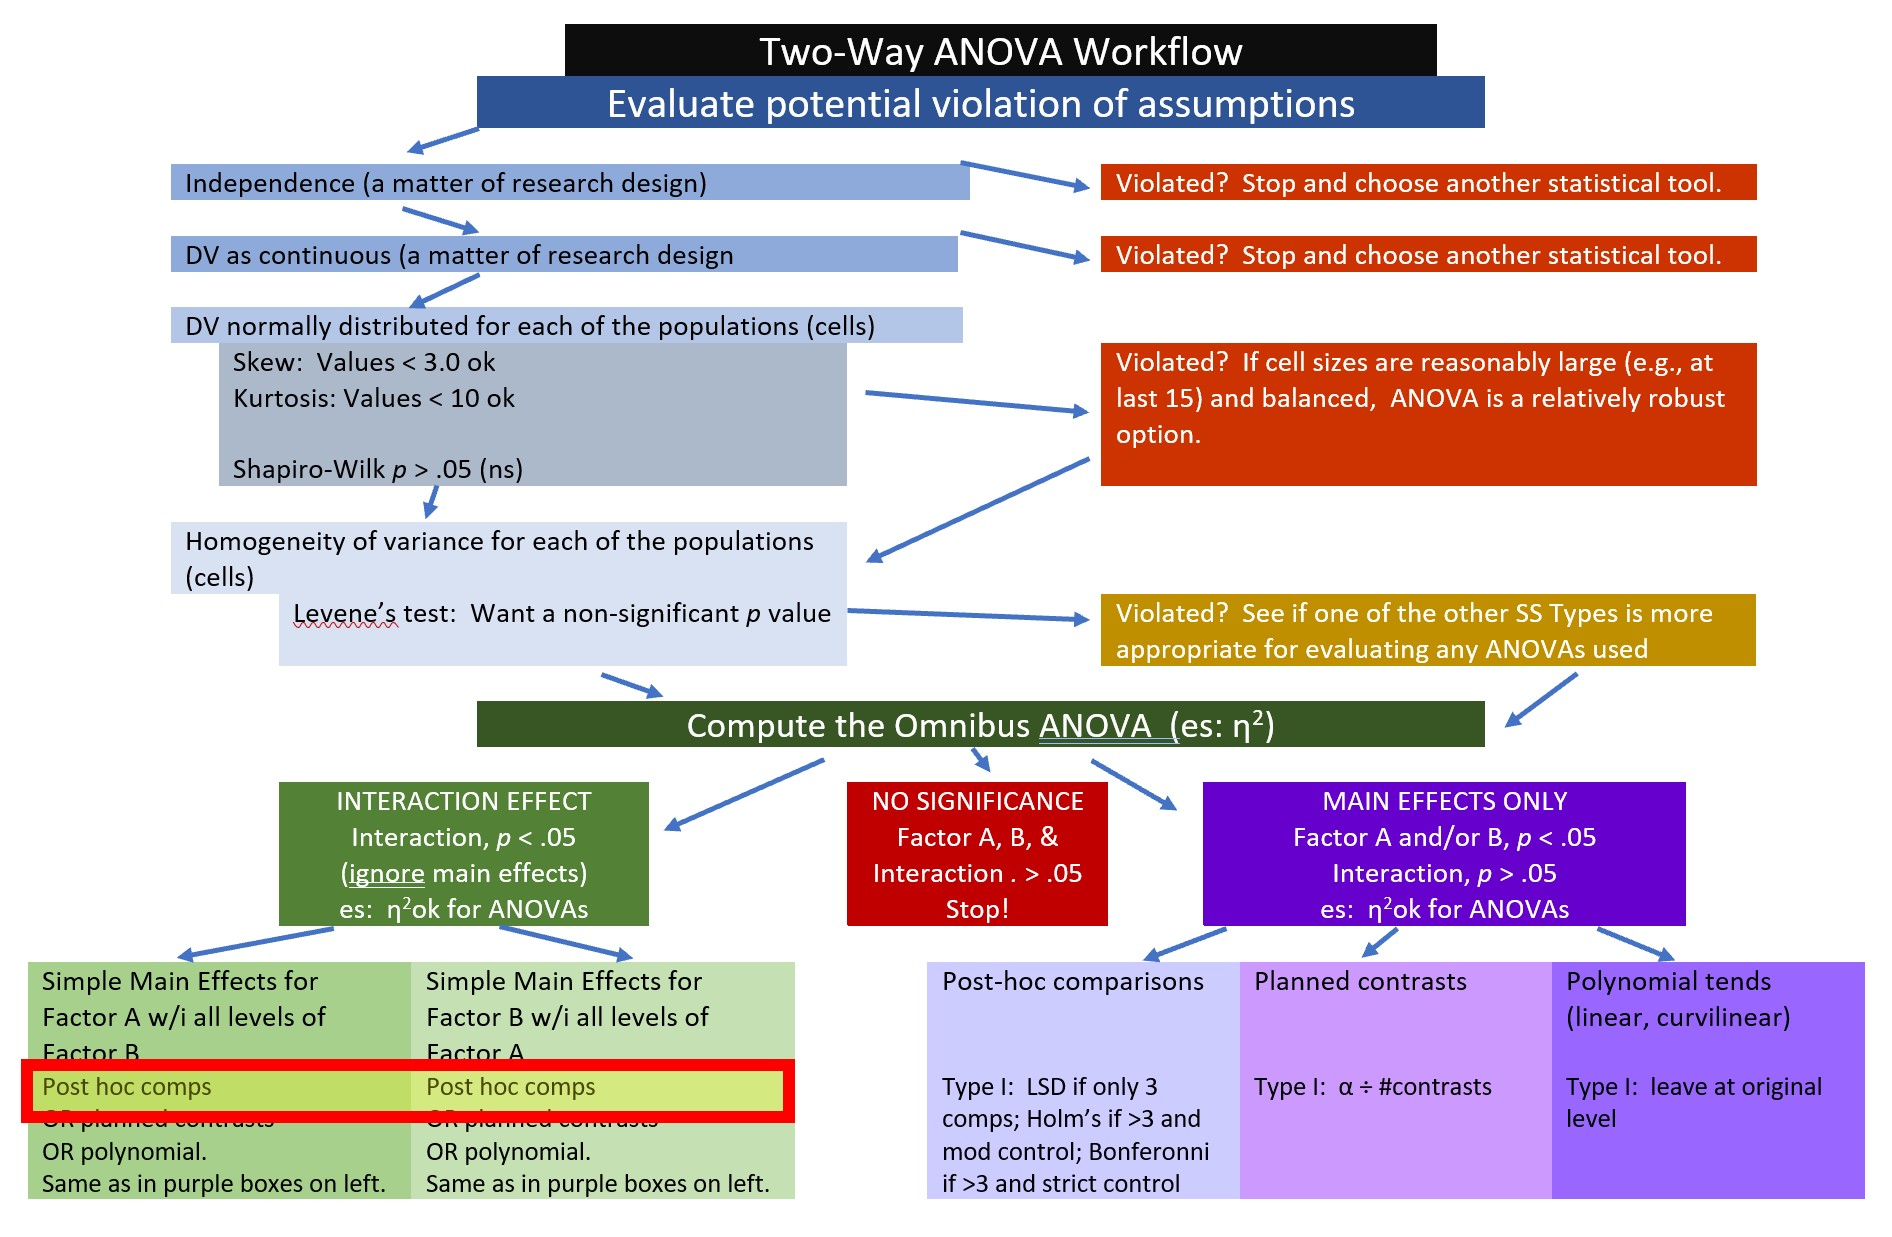
\includegraphics{images/factorial/WrkFlw_IntPH.jpg}
\caption{Image our place in the Two-Way ANOVA Workflow.}
\end{figure}

As the numbers of levels increase, post hoc comparisons become somewhat unwieldly. Even though this procedure produces them all, you can select which sensible number you want to compare and control for Type I error according to the number in that set.

With rater ethnicity (3 levels) and photo stimulus (2 levels), we have 6 groupings. When \emph{k} is the number of groups, the total number of paired comparisons is: k(k-1)*2

\begin{Shaded}
\begin{Highlighting}[]
\DecValTok{6} \SpecialCharTok{*}\NormalTok{ (}\DecValTok{6} \SpecialCharTok{{-}} \DecValTok{1}\NormalTok{)}\SpecialCharTok{/}\DecValTok{2}
\end{Highlighting}
\end{Shaded}

\begin{verbatim}
[1] 15
\end{verbatim}

Obtain the 15 post-hoc paired comparisons with the \emph{TukeyHSD()} function.

\begin{Shaded}
\begin{Highlighting}[]
\NormalTok{posthocs }\OtherTok{\textless{}{-}} \FunctionTok{TukeyHSD}\NormalTok{(TwoWay\_neg, }\AttributeTok{ordered =} \ConstantTok{TRUE}\NormalTok{)}
\NormalTok{posthocs}
\end{Highlighting}
\end{Shaded}

\begin{verbatim}
  Tukey multiple comparisons of means
    95% family-wise confidence level
    factor levels have been ordered

Fit: aov(formula = Negative ~ Rater * Photo, data = Ramdhani_df)

$Rater
                        diff         lwr       upr     p adj
Javanese-Dayaknese 0.5147954  0.02750358 1.0020872 0.0358235
Madurese-Dayaknese 0.8068425  0.32566283 1.2880222 0.0003629
Madurese-Javanese  0.2920471 -0.18222911 0.7663234 0.3124227

$Photo
                       diff       lwr      upr     p adj
Madurese-Dayaknese 0.726071 0.3987575 1.053385 0.0000262

$`Rater:Photo`
                                              diff         lwr       upr
Javanese:Dayaknese-Dayaknese:Dayaknese 0.706013072 -0.14743916 1.5594653
Dayaknese:Madurese-Dayaknese:Dayaknese 1.311568627  0.45811640 2.1650209
Madurese:Madurese-Dayaknese:Dayaknese  1.479735294  0.64726775 2.3122028
Madurese:Dayaknese-Dayaknese:Dayaknese 1.483077399  0.64060458 2.3255502
Javanese:Madurese-Dayaknese:Dayaknese  1.647182663  0.80470985 2.4896555
Dayaknese:Madurese-Javanese:Dayaknese  0.605555556 -0.23561614 1.4467273
Madurese:Madurese-Javanese:Dayaknese   0.773722222 -0.04615053 1.5935950
Madurese:Dayaknese-Javanese:Dayaknese  0.777064327 -0.05296553 1.6070942
Javanese:Madurese-Javanese:Dayaknese   0.941169591  0.11113973 1.7711995
Madurese:Madurese-Dayaknese:Madurese   0.168166667 -0.65170609 0.9880394
Madurese:Dayaknese-Dayaknese:Madurese  0.171508772 -0.65852109 1.0015386
Javanese:Madurese-Dayaknese:Madurese   0.335614035 -0.49441582 1.1656439
Madurese:Dayaknese-Madurese:Madurese   0.003342105 -0.80509532 0.8117795
Javanese:Madurese-Madurese:Madurese    0.167447368 -0.64099006 0.9758848
Javanese:Madurese-Madurese:Dayaknese   0.164105263 -0.65463115 0.9828417
                                           p adj
Javanese:Dayaknese-Dayaknese:Dayaknese 0.1652148
Dayaknese:Madurese-Dayaknese:Dayaknese 0.0002907
Madurese:Madurese-Dayaknese:Dayaknese  0.0000171
Madurese:Dayaknese-Dayaknese:Dayaknese 0.0000211
Javanese:Madurese-Dayaknese:Dayaknese  0.0000018
Dayaknese:Madurese-Javanese:Dayaknese  0.3005963
Madurese:Madurese-Javanese:Dayaknese   0.0760131
Madurese:Dayaknese-Javanese:Dayaknese  0.0802217
Javanese:Madurese-Javanese:Dayaknese   0.0166363
Madurese:Madurese-Dayaknese:Madurese   0.9911395
Madurese:Dayaknese-Dayaknese:Madurese  0.9908344
Javanese:Madurese-Dayaknese:Madurese   0.8482970
Madurese:Dayaknese-Madurese:Madurese   1.0000000
Javanese:Madurese-Madurese:Madurese    0.9907331
Javanese:Madurese-Madurese:Dayaknese   0.9920328
\end{verbatim}

If we want to consider all 15 pairwise comparisons and also control for Type I error, a Holm's sequential Bonerroni \citep{green_using_2014} will help us take a middle-of-the-road approach (not as strict as .05/15 with the traditional Bonferroni; not as lenient as ``none'') to managing Type I error.

With the Holms, we rank order the \emph{p} values associated with the 15 comparisons in order from lowest (e.g., .0000018) to highest (e.g., 1.000). The first \emph{p} value is evaluated with the most strict criterion (.05/15; the traditional Bonferonni approach). Then, each successive comparison calculates the \emph{p} value by using the number of \emph{remaining} comparisons as the denominator (e.g., .05/14, .05/13, .05/12). As the \emph{p} values rise and the alpha levels relax, there will be a cut-point where remaining comparisons are not statistically significant.

\begin{Shaded}
\begin{Highlighting}[]
\FloatTok{0.05}\SpecialCharTok{/}\DecValTok{15}
\end{Highlighting}
\end{Shaded}

\begin{verbatim}
[1] 0.003333333
\end{verbatim}

\begin{Shaded}
\begin{Highlighting}[]
\FloatTok{0.05}\SpecialCharTok{/}\DecValTok{14}
\end{Highlighting}
\end{Shaded}

\begin{verbatim}
[1] 0.003571429
\end{verbatim}

To facilitate this contrast, let's extract the 15 TukeyHSD tests and work with them in Excel.

First, obtain the structure of the \emph{posthoc} object

\begin{Shaded}
\begin{Highlighting}[]
\FunctionTok{str}\NormalTok{(posthocs)}
\end{Highlighting}
\end{Shaded}

\begin{verbatim}
List of 3
 $ Rater      : num [1:3, 1:4] 0.5148 0.8068 0.292 0.0275 0.3257 ...
  ..- attr(*, "dimnames")=List of 2
  .. ..$ : chr [1:3] "Javanese-Dayaknese" "Madurese-Dayaknese" "Madurese-Javanese"
  .. ..$ : chr [1:4] "diff" "lwr" "upr" "p adj"
 $ Photo      : num [1, 1:4] 0.726071 0.3987575 1.0533845 0.0000262
  ..- attr(*, "dimnames")=List of 2
  .. ..$ : chr "Madurese-Dayaknese"
  .. ..$ : chr [1:4] "diff" "lwr" "upr" "p adj"
 $ Rater:Photo: num [1:15, 1:4] 0.706 1.312 1.48 1.483 1.647 ...
  ..- attr(*, "dimnames")=List of 2
  .. ..$ : chr [1:15] "Javanese:Dayaknese-Dayaknese:Dayaknese" "Dayaknese:Madurese-Dayaknese:Dayaknese" "Madurese:Madurese-Dayaknese:Dayaknese" "Madurese:Dayaknese-Dayaknese:Dayaknese" ...
  .. ..$ : chr [1:4] "diff" "lwr" "upr" "p adj"
 - attr(*, "class")= chr [1:2] "TukeyHSD" "multicomp"
 - attr(*, "orig.call")= language aov(formula = Negative ~ Rater * Photo, data = Ramdhani_df)
 - attr(*, "conf.level")= num 0.95
 - attr(*, "ordered")= logi TRUE
\end{verbatim}

\begin{Shaded}
\begin{Highlighting}[]
\FunctionTok{write.csv}\NormalTok{(posthocs}\SpecialCharTok{$}\StringTok{"Rater:Photo"}\NormalTok{, }\StringTok{"posthocsOUT.csv"}\NormalTok{)}
\end{Highlighting}
\end{Shaded}

In Excel, I would sort my results by their \emph{p} values (low to high) and consider my threshold (\emph{p} \textless{} .0033) to determine which effects were statistically significant. Using the strictest criteria of \emph{p} \textless{} .0033, we would have four statistically significant values.

\begin{figure}
\centering
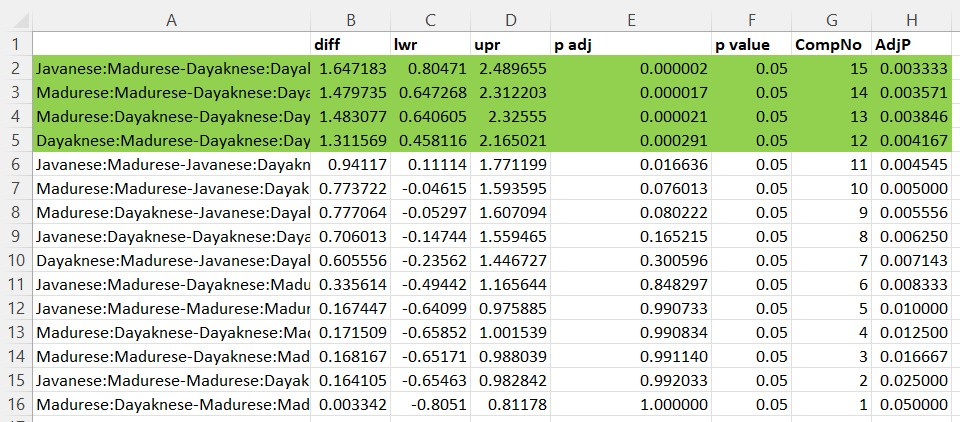
\includegraphics{images/factorial/Holmsequential.jpg}
\caption{Image of the results of the Holms sequential Bonferroni.}
\end{figure}

I would ask, ``Is this what we want?'' Similar to the simple main effects we just tested, I am interested in two sets of comparisons:

First, how are the two sets of photos (Madurese and Dayaknese) rated within each set of raters.

\begin{itemize}
\tightlist
\item
  Javanese:Madurese - Javanese:Dayaknese
\item
  Dayaknese:Madurese - Dayaknese:Dayaknese
\item
  Madurese:Madurese - Madurese:Dayaknese
\end{itemize}

Second, focused on each photo, what are the relative ratings.

\begin{itemize}
\tightlist
\item
  Javanese:Madurese - Dayaknese:Madurese
\item
  Madurese: Madurese - Dayaknese:Madurese
\item
  Javanese:Dayaknese - Dayaknese:Dayaknese
\item
  Madurese: Dayaknese - Dayaknese:Dayaknese
\end{itemize}

This is only seven sets of comparisons and would considerably reduce the alpha:

\begin{Shaded}
\begin{Highlighting}[]
\FloatTok{0.05}\SpecialCharTok{/}\DecValTok{7}
\end{Highlighting}
\end{Shaded}

\begin{verbatim}
[1] 0.007142857
\end{verbatim}

Below I have greyed-out the comparisons that are less interesting to me and left the seven that are my focal interest. I have highlighted in green the two comparisons that are statistically significant based on the Holms' sequential criteria. In this case, it does not make any difference in our interpretation of these focal predictors.

\begin{figure}
\centering
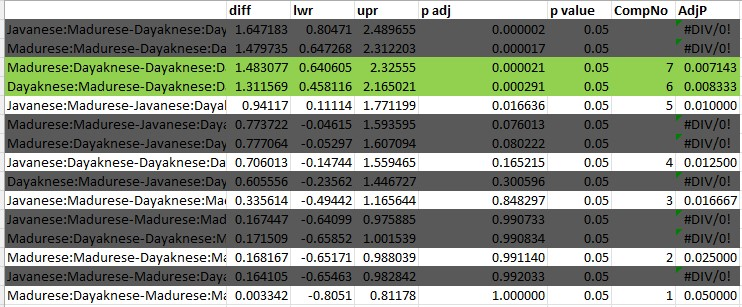
\includegraphics{images/factorial/HolmsSelect.jpg}
\caption{Image of the results of the Holms sequential Bonferroni.}
\end{figure}

\hypertarget{option-4-polynomial-trends}{%
\subsubsection{Option \#4 polynomial trends}\label{option-4-polynomial-trends}}

In the context of the significant interaction effect, we might also be interested in polynomial trends for any simple main effects where 3 or more cells are compared.

Why? If there are only two cells being compared, then the significance of that has already been tested and if significant, it is also a significant linear effect (because the shape between any two points is a line). Below is a figure of where the polynomial test of an interaction effect may fall in the process.

At the outset, let me acknowledge that this is not the best example to demonstrate a polynomial trend. Why? We do not necessarily have an ordered prediction across categories for this vignette. Other research scenarios (e.g., when dosage is none, low, high) are more readily suited for this approach.

\begin{figure}
\centering
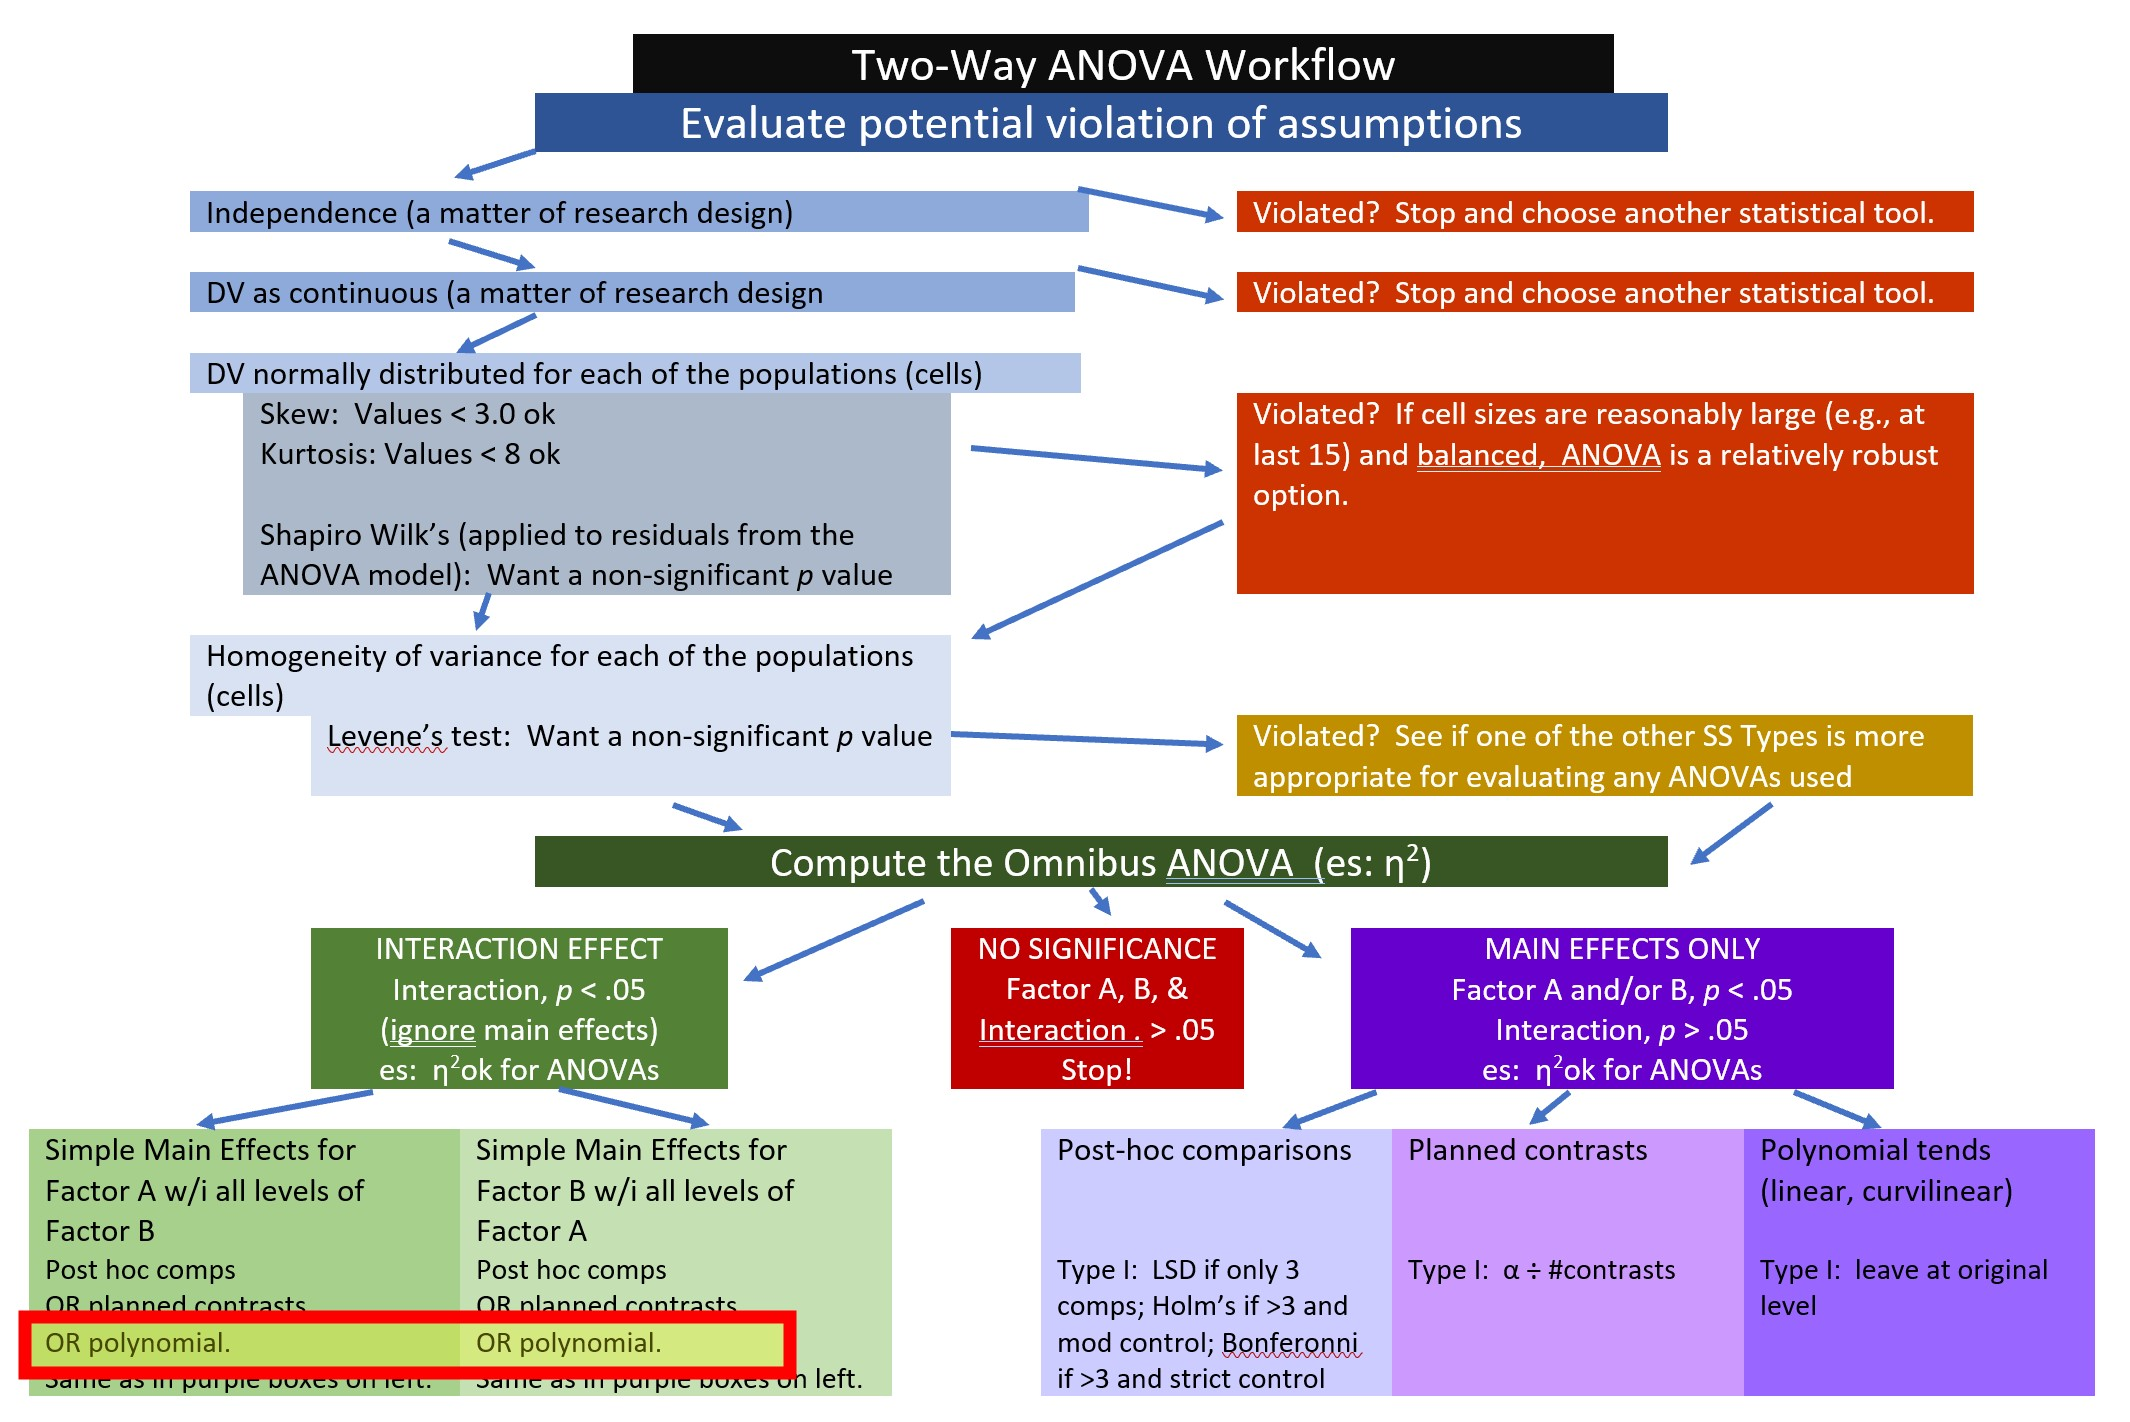
\includegraphics{images/factorial/WrkFlw_Poly.jpg}
\caption{Image our place in the Two-Way ANOVA Workflow.}
\end{figure}

In our example, Rater has three groups. Thus, we could evaluate a polynomial for the simple main effect of ethnicity of the rater within photo stimulus (separately for the photos of the Dayaknese and Madurese). We conduct these separately for Dayaknese, Madurese, and Javanese groups.

In the event that more than one polynomial trend select the higher one. For example, if both linear and quadratic are selected, interpret the quadratic trend

\begin{Shaded}
\begin{Highlighting}[]
\FunctionTok{contrasts}\NormalTok{(Dayaknese\_Ph}\SpecialCharTok{$}\NormalTok{Rater) }\OtherTok{\textless{}{-}} \FunctionTok{contr.poly}\NormalTok{(}\DecValTok{3}\NormalTok{)}
\NormalTok{poly\_Dy }\OtherTok{\textless{}{-}} \FunctionTok{aov}\NormalTok{(Negative }\SpecialCharTok{\textasciitilde{}}\NormalTok{ Rater, }\AttributeTok{data =}\NormalTok{ Dayaknese\_Ph)}
\FunctionTok{summary.lm}\NormalTok{(poly\_Dy)}
\end{Highlighting}
\end{Shaded}

\begin{verbatim}
Call:
aov(formula = Negative ~ Rater, data = Dayaknese_Ph)

Residuals:
    Min      1Q  Median      3Q     Max 
-1.8948 -0.5463 -0.1098  0.5155  2.1402 

Coefficients:
            Estimate Std. Error t value             Pr(>|t|)    
(Intercept)  2.54746    0.11744  21.693 < 0.0000000000000002 ***
Rater.L      1.04869    0.20351   5.153           0.00000419 ***
Rater.Q      0.02901    0.20330   0.143                0.887    
---
Signif. codes:  0 '***' 0.001 '**' 0.01 '*' 0.05 '.' 0.1 ' ' 1

Residual standard error: 0.8621 on 51 degrees of freedom
Multiple R-squared:  0.3432,    Adjusted R-squared:  0.3174 
F-statistic: 13.32 on 2 and 51 DF,  p-value: 0.00002211
\end{verbatim}

Results of a polynomial trend analysis indicated a statistically significant linear trend for evaluation of the Dayaknese photos across the three raters \emph{t} (51) = 5.153, \emph{p} \textless{} .001.

\begin{Shaded}
\begin{Highlighting}[]
\FunctionTok{contrasts}\NormalTok{(Madurese\_Ph}\SpecialCharTok{$}\NormalTok{Rater) }\OtherTok{\textless{}{-}} \FunctionTok{contr.poly}\NormalTok{(}\DecValTok{3}\NormalTok{)}
\NormalTok{poly\_Md }\OtherTok{\textless{}{-}} \FunctionTok{aov}\NormalTok{(Negative }\SpecialCharTok{\textasciitilde{}}\NormalTok{ Rater, }\AttributeTok{data =}\NormalTok{ Madurese\_Ph)}
\FunctionTok{summary.lm}\NormalTok{(poly\_Md)}
\end{Highlighting}
\end{Shaded}

\begin{verbatim}
Call:
aov(formula = Negative ~ Rater, data = Madurese_Ph)

Residuals:
     Min       1Q   Median       3Q      Max 
-2.08650 -0.54395  0.01367  0.35905  2.34350 

Coefficients:
            Estimate Std. Error t value            Pr(>|t|)    
(Intercept)   3.2973     0.1161  28.391 <0.0000000000000002 ***
Rater.L       0.1189     0.2012   0.591               0.557    
Rater.Q      -0.2054     0.2011  -1.021               0.312    
---
Signif. codes:  0 '***' 0.001 '**' 0.01 '*' 0.05 '.' 0.1 ' ' 1

Residual standard error: 0.876 on 54 degrees of freedom
Multiple R-squared:  0.02451,   Adjusted R-squared:  -0.01162 
F-statistic: 0.6785 on 2 and 54 DF,  p-value: 0.5116
\end{verbatim}

Results of a polynomial trend analysis were non-significant when ethnicity of the rater was evaluated when rating Madurese photos.

\hypertarget{investigating-main-effects}{%
\section{Investigating Main Effects}\label{investigating-main-effects}}

We now focus on the possibility that there might be significant main effects, but a non-significant interaction effect. We only interpret main effects when there is a non-significant interaction effect. Why? Because in the presence of a significant interaction effect, the main effect will not tell a complete story. \emph{(And, if we didn't specify a correct model, we still might have an incomplete story. But that's another issue.)} Here's where we are on the workflow.

\begin{figure}
\centering
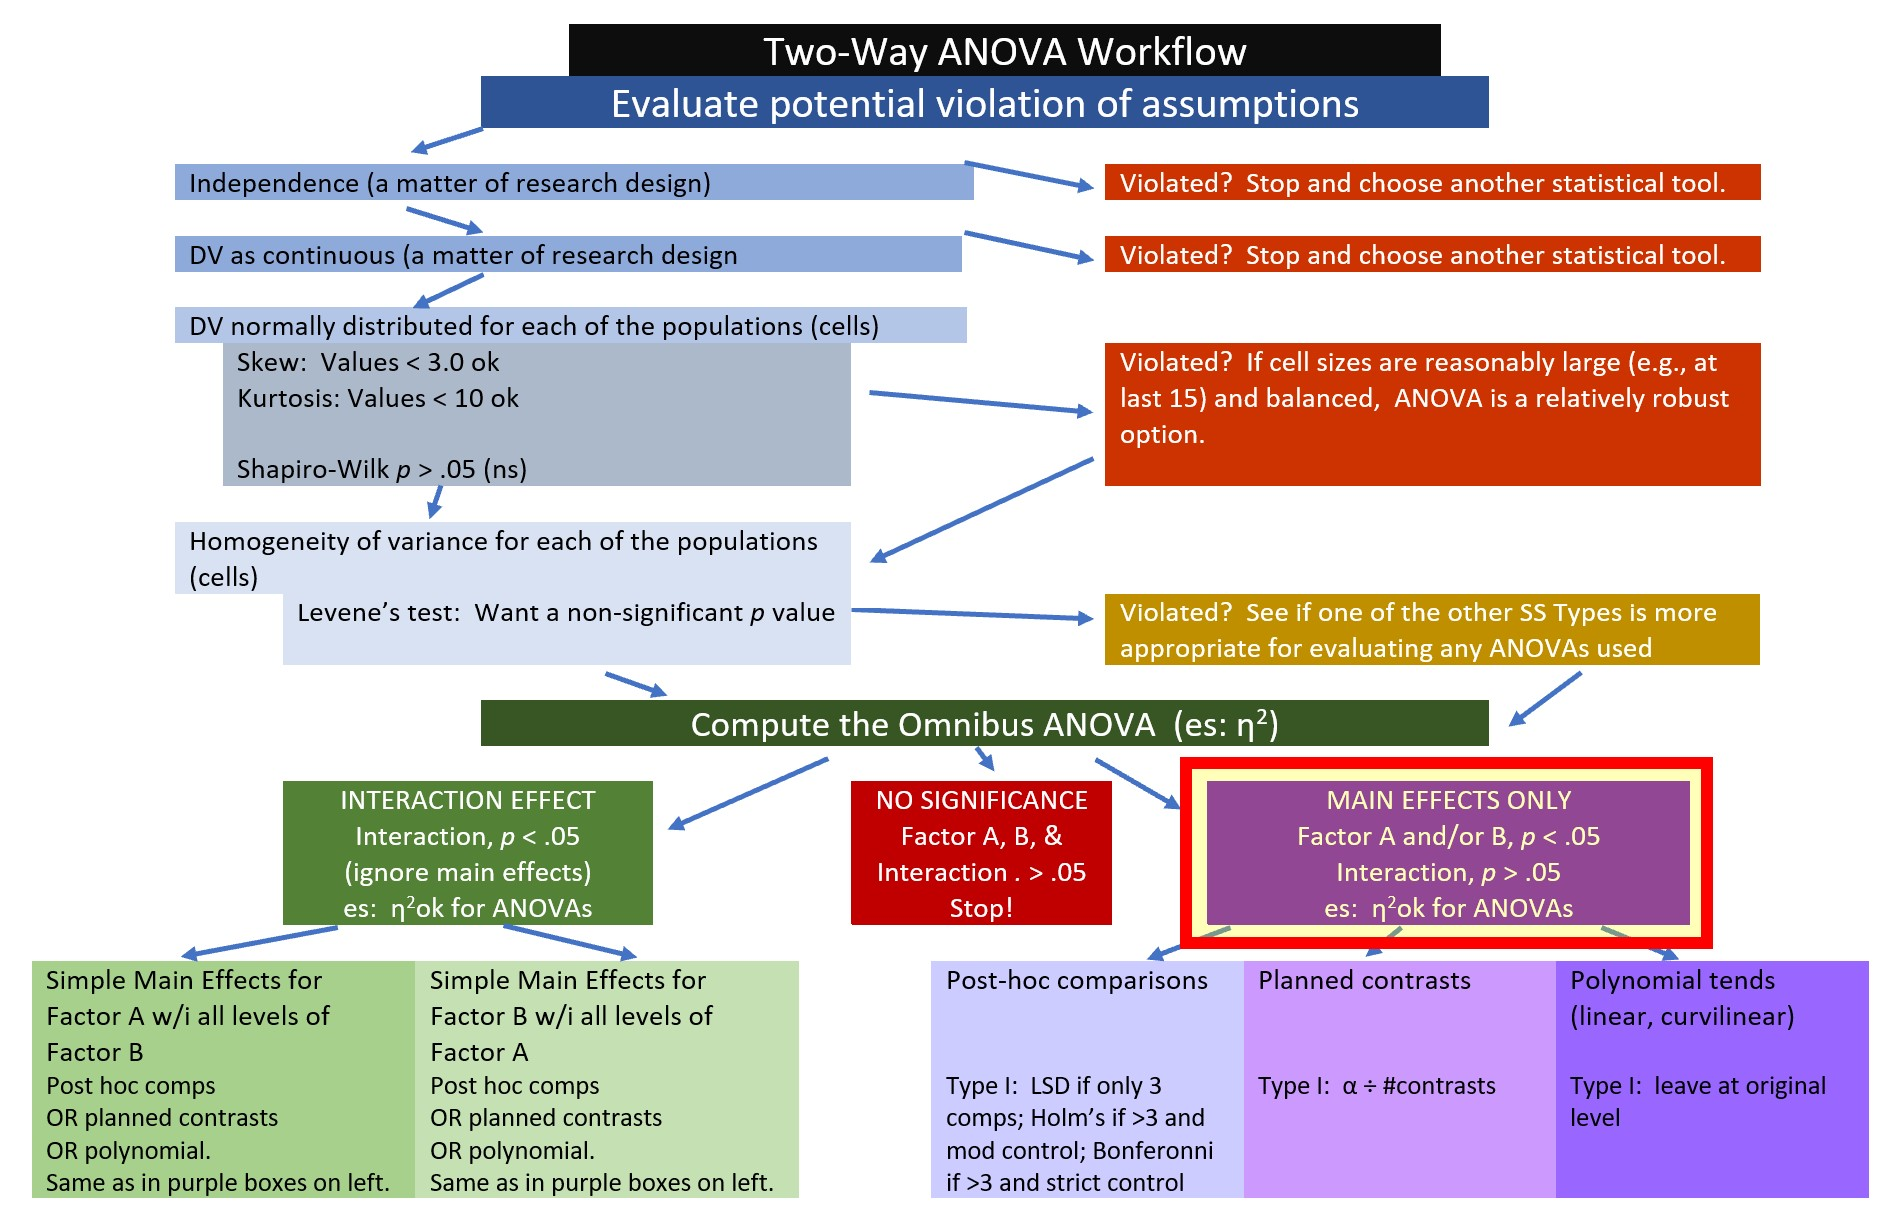
\includegraphics{images/factorial/WayWrkFlw_Main.jpg}
\caption{Image our place in the Two-Way ANOVA Workflow.}
\end{figure}

Recall that main effects are the \emph{marginal means} -- that is the effects of Factor A \emph{collapsed across} all the levels of Factor B.

If the main effect has only two levels (e.g., the ratings of the Dayaknese and Madurese photos):

\begin{itemize}
\tightlist
\item
  the comparison was already ignoring/including all levels of the rater ethnicity factor (Dayaknese, Madurese, Javanese),
\item
  it was only a comparison of two cells (Dayaknese rater, Madurese rater), therefore
\item
  there is no need for further follow-up.
\end{itemize}

If the main effect has three or more levels (e.g,. ethnicity of rater with Dayaknese, Madurese, Javanese levels), then you would follow-up with one or more of the myriad of options. In this class we have focused on three:

\begin{itemize}
\tightlist
\item
  planned contrasts
\item
  posthoc comparisons (all possible cells)
\item
  polynomial
\end{itemize}

I will demonstrate how to do each as follow-up to a \emph{pretend} scenario where a main effect (but not an interaction) had been significant. I will write up the portion that would be inserted in an APA style results section.

Essentially, we treat these main effect analyses as the follow-up to a significant one-way ANOVA evaluating, in our case, the ethnicity of the Rater.

\begin{Shaded}
\begin{Highlighting}[]
\NormalTok{RaterMain }\OtherTok{\textless{}{-}} \FunctionTok{aov}\NormalTok{(Negative }\SpecialCharTok{\textasciitilde{}}\NormalTok{ Rater, }\AttributeTok{data =}\NormalTok{ Ramdhani\_df)  }\CommentTok{\#DV \textasciitilde{} IV I say, \textquotesingle{}DV by IV\textquotesingle{}}
\FunctionTok{model.tables}\NormalTok{(RaterMain)  }\CommentTok{\#ANOVA output}
\end{Highlighting}
\end{Shaded}

\begin{verbatim}
Tables of effects

 Rater 
    Dayaknese Javanese Madurese
      -0.4551  0.05971   0.3518
rep   35.0000 37.00000  39.0000
\end{verbatim}

\begin{Shaded}
\begin{Highlighting}[]
\FunctionTok{summary}\NormalTok{(RaterMain)}
\end{Highlighting}
\end{Shaded}

\begin{verbatim}
             Df Sum Sq Mean Sq F value  Pr(>F)   
Rater         2  12.21   6.103   6.426 0.00231 **
Residuals   108 102.57   0.950                   
---
Signif. codes:  0 '***' 0.001 '**' 0.01 '*' 0.05 '.' 0.1 ' ' 1
\end{verbatim}

\begin{Shaded}
\begin{Highlighting}[]
\NormalTok{lsr}\SpecialCharTok{::}\FunctionTok{etaSquared}\NormalTok{(RaterMain)}
\end{Highlighting}
\end{Shaded}

\begin{verbatim}
         eta.sq eta.sq.part
Rater 0.1063485   0.1063485
\end{verbatim}

A boxplot representing this main effect may help convey how the main effect of Rater (collapsed across Photo) is different than an interaction effect.

\begin{Shaded}
\begin{Highlighting}[]
\NormalTok{ggpubr}\SpecialCharTok{::}\FunctionTok{ggboxplot}\NormalTok{(Ramdhani\_df, }\AttributeTok{x =} \StringTok{"Rater"}\NormalTok{, }\AttributeTok{y =} \StringTok{"Negative"}\NormalTok{, }\AttributeTok{xlab =} \StringTok{"Ethnicity of Rater"}\NormalTok{,}
    \AttributeTok{ylab =} \StringTok{"Negative Reaction"}\NormalTok{)}
\end{Highlighting}
\end{Shaded}

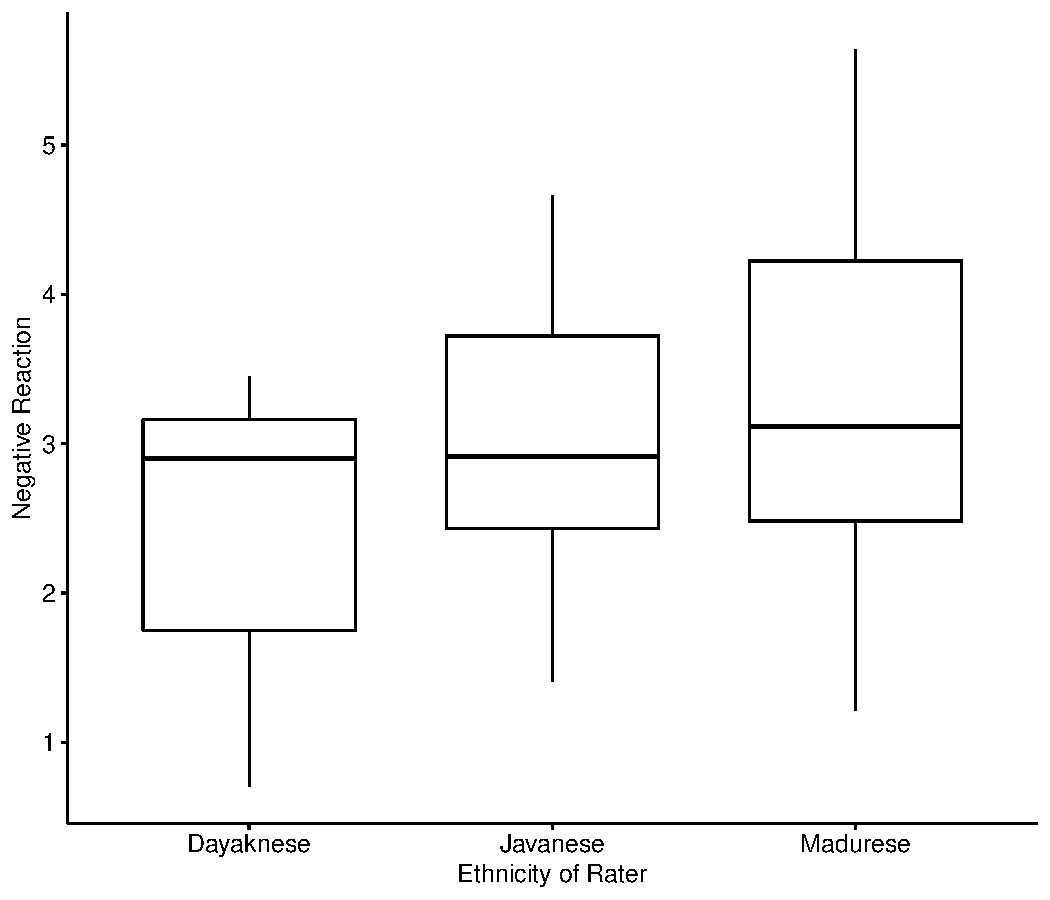
\includegraphics{ReCenterPsychStats_files/figure-latex/unnamed-chunk-169-1.pdf}

\hypertarget{follow-up-with-all-post-hocs}{%
\subsection{Follow-up with all Post-Hocs}\label{follow-up-with-all-post-hocs}}

An easy possibility is to follow-up with all possible post-hocs. In the main effect case, these are far simpler than where we conducted all possile posthocs for the interaction effect (remember the Holms sequential Bonferroni?).

Here is a reminder of our location on the workflow.

\begin{figure}
\centering
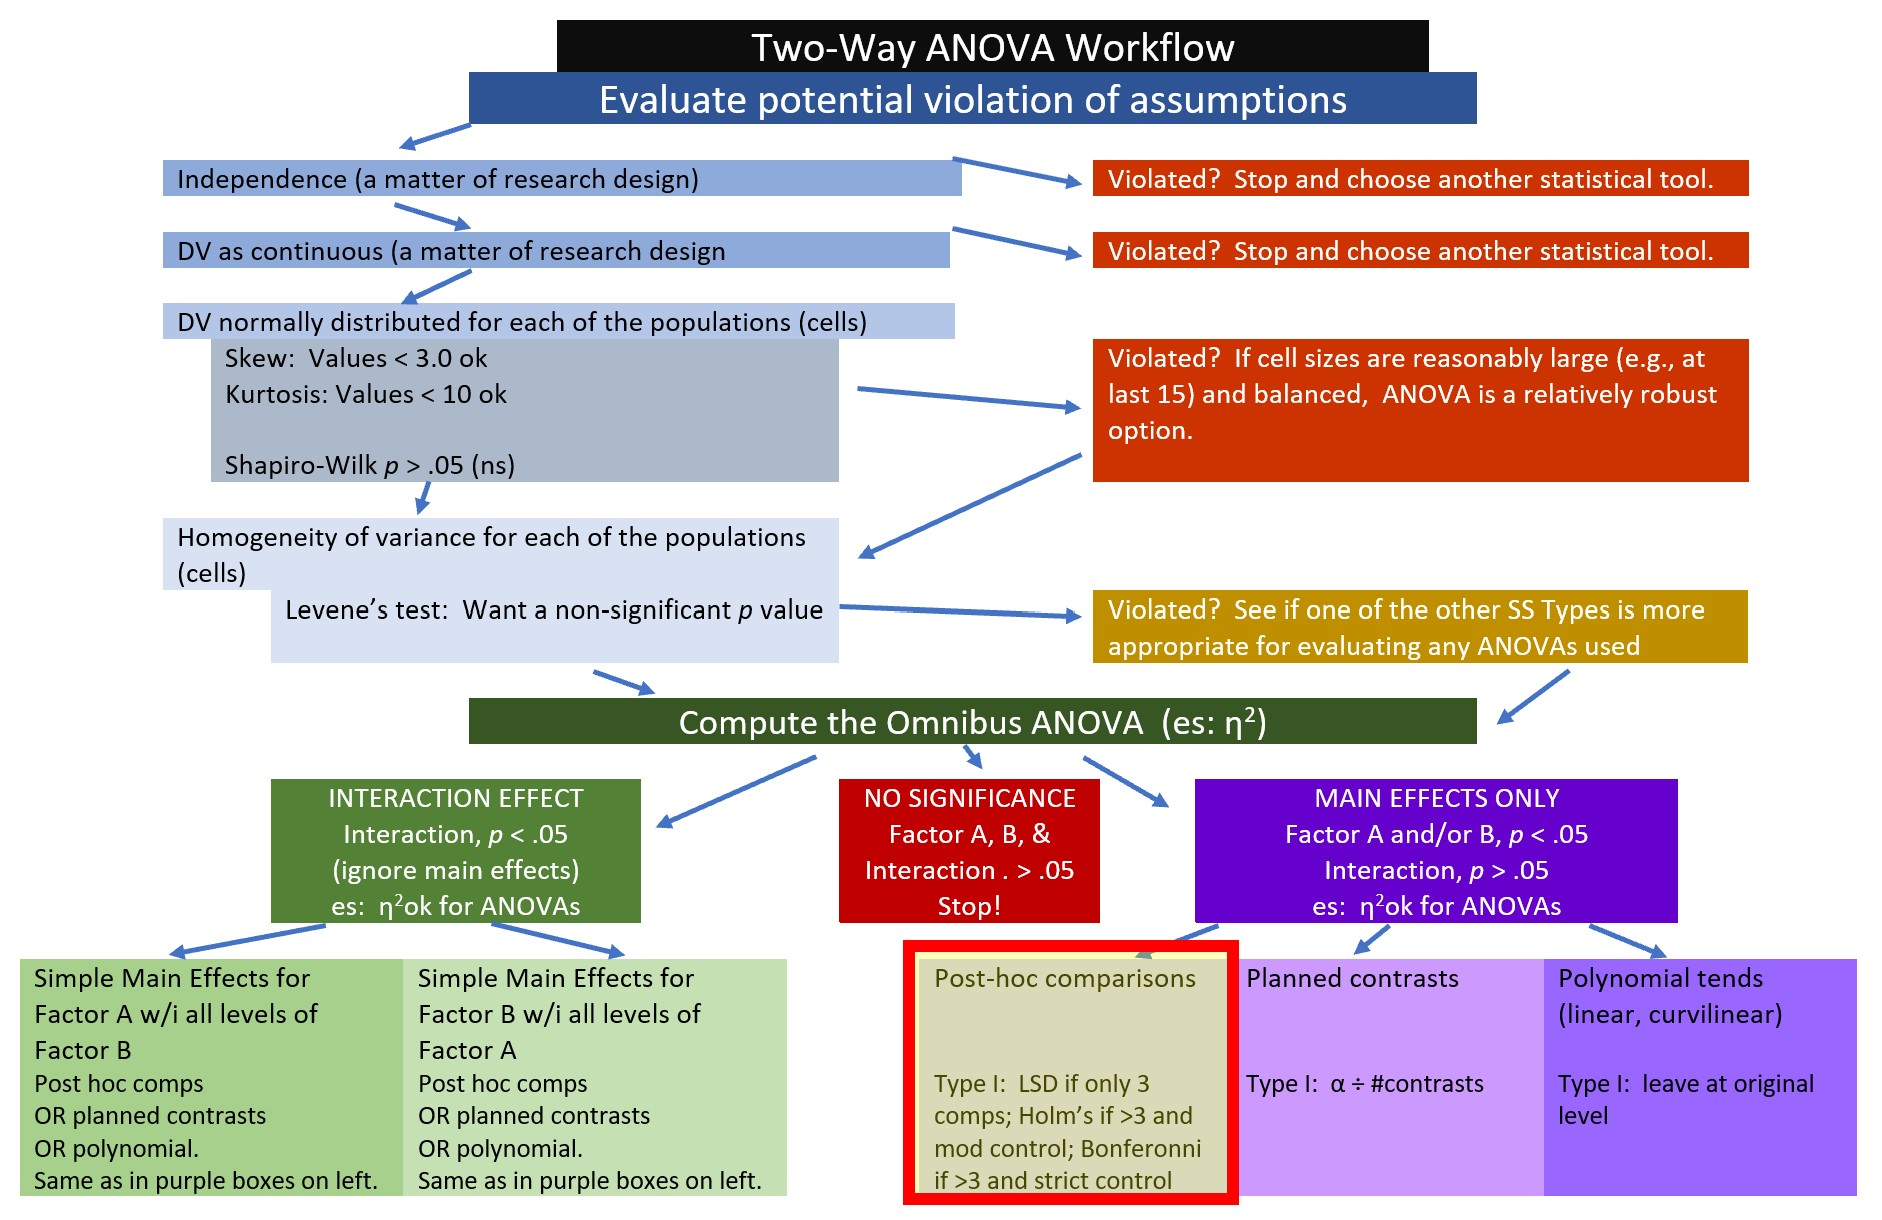
\includegraphics{images/factorial/wfMain_PH.jpg}
\caption{Image our place in the Two-Way ANOVA Workflow.}
\end{figure}

The \emph{TukeyHSD()} function produces posthoc comparisons by providing the mean difference, a 95\% confidence interval of those differences, and the associated \emph{p} value.

\begin{Shaded}
\begin{Highlighting}[]
\FunctionTok{TukeyHSD}\NormalTok{(RaterMain, }\AttributeTok{ordered =} \ConstantTok{TRUE}\NormalTok{)}
\end{Highlighting}
\end{Shaded}

\begin{verbatim}
  Tukey multiple comparisons of means
    95% family-wise confidence level
    factor levels have been ordered

Fit: aov(formula = Negative ~ Rater, data = Ramdhani_df)

$Rater
                        diff         lwr       upr     p adj
Javanese-Dayaknese 0.5147954 -0.03128503 1.0608758 0.0690316
Madurese-Dayaknese 0.8068425  0.26761161 1.3460734 0.0016135
Madurese-Javanese  0.2920471 -0.23944747 0.8235417 0.3950430
\end{verbatim}

Results suggest there were statistically significant differences (\emph{p} \textless{} .05) between the Madurese and Dayaknese. These differences, though, would have been when rating \emph{all} photos. This analysis disregards the ethnicity portrayed in the photo.

\hypertarget{follow-up-with-planned-contrasts}{%
\subsection{Follow-up with planned contrasts}\label{follow-up-with-planned-contrasts}}

We generally try for \emph{orthogonal} contrasts so that the partitioning of variance is independent (clean, not overlapping). Planned contrasts are a great way to do this. Here's where we are in the workflow.

\begin{figure}
\centering
\includegraphics{images/factorial/wfMain_Plnd.jpg}
\caption{Image our place in the Two-Way ANOVA Workflow.}
\end{figure}

If you aren't extremely careful about your order-of-operations in R, it can confuse objects, so I have named these contrasts \emph{main\_c1} and \emph{main\_c2} to remind myself that they refer to the main effect of ethnicity of the rater.

In this hypothetical scenario (remember we are pretending we are in the circumstance of a non-significant interaction effect but a significant main effect), I am:

\begin{itemize}
\tightlist
\item
  Constrast \#1: comparing the DV for the Javanese rater to the combined Dayaknese and Madurese raters.
\item
  Contrast \#2: comparing the DV for the Dayaknese and Madurese raters.
\end{itemize}

These are orthogonal because:

\begin{itemize}
\tightlist
\item
  there are \emph{k} - 1 comparisons, and
\item
  once a contrast is isolated (i.e., the Javanese rater in contrast \#1) it cannot be used again

  \begin{itemize}
  \tightlist
  \item
    Recall the piece of cake analogy: once you take out a piece of the cake, you really can't put it back in
  \end{itemize}
\end{itemize}

\begin{Shaded}
\begin{Highlighting}[]
\CommentTok{\# Contrast1 compares Control against the combined effects of Low and}
\CommentTok{\# High.}
\NormalTok{main\_c1 }\OtherTok{\textless{}{-}} \FunctionTok{c}\NormalTok{(}\DecValTok{1}\NormalTok{, }\SpecialCharTok{{-}}\DecValTok{2}\NormalTok{, }\DecValTok{1}\NormalTok{)}

\CommentTok{\# Contrast2 excludes Control; compares Low to High.}
\NormalTok{main\_c2 }\OtherTok{\textless{}{-}} \FunctionTok{c}\NormalTok{(}\SpecialCharTok{{-}}\DecValTok{1}\NormalTok{, }\DecValTok{0}\NormalTok{, }\DecValTok{1}\NormalTok{)}
\FunctionTok{contrasts}\NormalTok{(Ramdhani\_df}\SpecialCharTok{$}\NormalTok{Rater) }\OtherTok{\textless{}{-}} \FunctionTok{cbind}\NormalTok{(main\_c1, main\_c2)}
\FunctionTok{contrasts}\NormalTok{(Ramdhani\_df}\SpecialCharTok{$}\NormalTok{Rater)}
\end{Highlighting}
\end{Shaded}

\begin{verbatim}
          main_c1 main_c2
Dayaknese       1      -1
Javanese       -2       0
Madurese        1       1
\end{verbatim}

Then we run the contrast

\begin{Shaded}
\begin{Highlighting}[]
\NormalTok{mainPlanned }\OtherTok{\textless{}{-}} \FunctionTok{aov}\NormalTok{(Negative }\SpecialCharTok{\textasciitilde{}}\NormalTok{ Rater, }\AttributeTok{data =}\NormalTok{ Ramdhani\_df)}
\FunctionTok{summary.lm}\NormalTok{(mainPlanned)}
\end{Highlighting}
\end{Shaded}

\begin{verbatim}
Call:
aov(formula = Negative ~ Rater, data = Ramdhani_df)

Residuals:
     Min       1Q   Median       3Q      Max 
-2.08813 -0.74921  0.05792  0.71482  2.34187 

Coefficients:
             Estimate Std. Error t value             Pr(>|t|)    
(Intercept)   2.93283    0.09259  31.676 < 0.0000000000000002 ***
Ratermain_c1 -0.03712    0.06544  -0.567             0.571670    
Ratermain_c2  0.40342    0.11345   3.556             0.000561 ***
---
Signif. codes:  0 '***' 0.001 '**' 0.01 '*' 0.05 '.' 0.1 ' ' 1

Residual standard error: 0.9745 on 108 degrees of freedom
Multiple R-squared:  0.1063,    Adjusted R-squared:  0.0898 
F-statistic: 6.426 on 2 and 108 DF,  p-value: 0.002307
\end{verbatim}

\begin{Shaded}
\begin{Highlighting}[]
\FunctionTok{contrasts}\NormalTok{(Ramdhani\_df}\SpecialCharTok{$}\NormalTok{Rater) }\OtherTok{\textless{}{-}} \FunctionTok{cbind}\NormalTok{(}\FunctionTok{c}\NormalTok{(}\DecValTok{1}\NormalTok{, }\SpecialCharTok{{-}}\DecValTok{2}\NormalTok{, }\DecValTok{1}\NormalTok{), }\FunctionTok{c}\NormalTok{(}\SpecialCharTok{{-}}\DecValTok{1}\NormalTok{, }\DecValTok{0}\NormalTok{, }\DecValTok{1}\NormalTok{))}
\end{Highlighting}
\end{Shaded}

These planned contrasts show that when the Javanese raters are compared to the combined Dayaknese and Madurese raters, there was a non significant difference, \emph{t}(108) = -0.567, \emph{p} = .572. However, there were significant differences between Dayaknese and Javanese raters, \emph{t}(108) = 3.556, \emph{p} \textless{} .001.

\hypertarget{polynomial-trends}{%
\subsection{Polynomial Trends}\label{polynomial-trends}}

Polynomial contrasts let us see if there is a linear (or curvilinear) pattern to the data. To detect a trend, the data must be coded in an ascending order\ldots and it needs to be a sensible comparison. Here's where this would fall in our workflow.

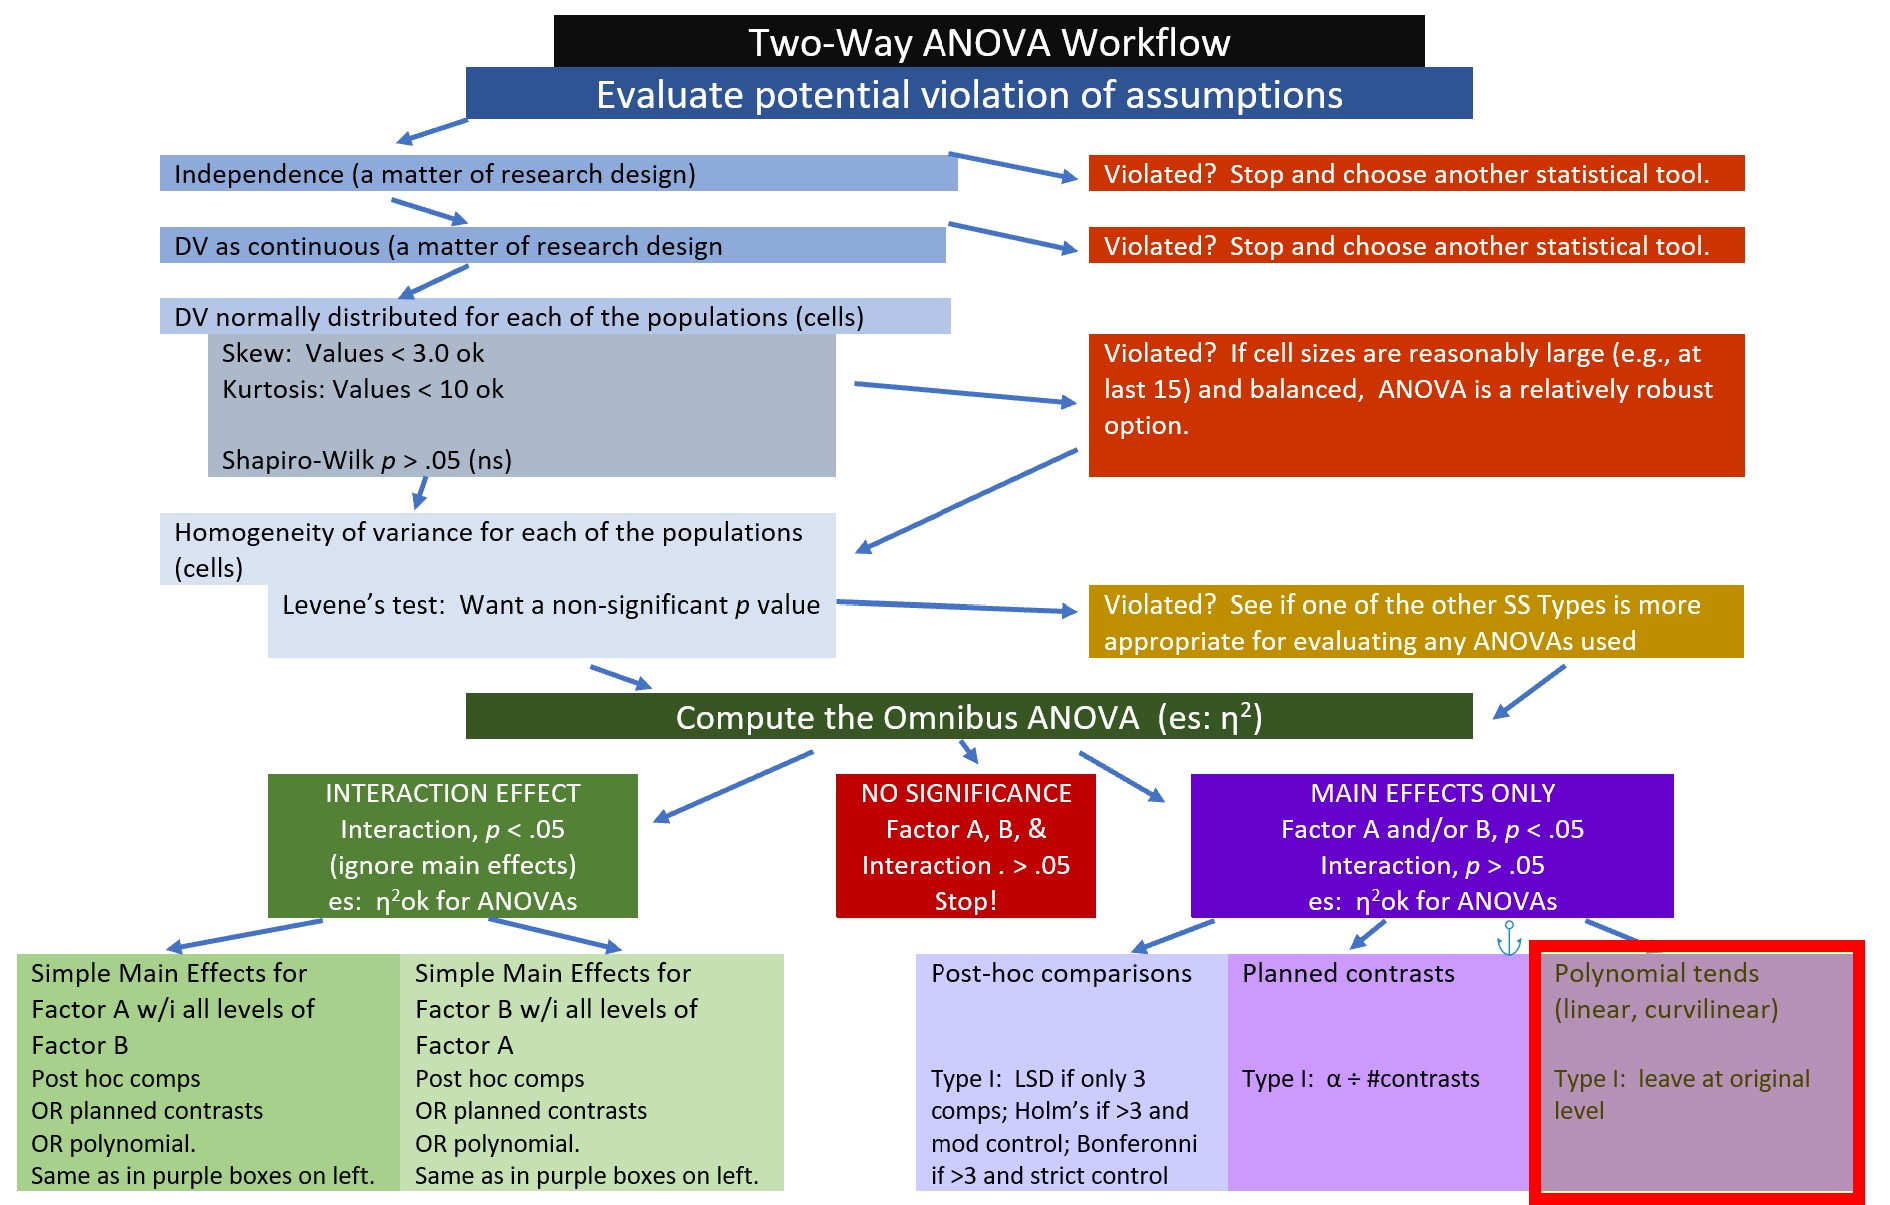
\includegraphics{images/factorial/wfMain_Poly.jpg}
Because these three ethnic groups are not \emph{ordered} in the same way as would an experiment involving dosage (e.g,. placebo, lo dose, hi dose), evaluation of the polynomial trend is not really justified (even though it is statistically possible). None-the-less, I will demonstrate how it is conducted.

\begin{Shaded}
\begin{Highlighting}[]
\FunctionTok{contrasts}\NormalTok{(Ramdhani\_df}\SpecialCharTok{$}\NormalTok{Rater) }\OtherTok{\textless{}{-}} \FunctionTok{contr.poly}\NormalTok{(}\DecValTok{3}\NormalTok{)}
\NormalTok{mainTrend }\OtherTok{\textless{}{-}} \FunctionTok{aov}\NormalTok{(Negative }\SpecialCharTok{\textasciitilde{}}\NormalTok{ Rater, }\AttributeTok{data =}\NormalTok{ Ramdhani\_df)}
\FunctionTok{summary.lm}\NormalTok{(mainTrend)}
\end{Highlighting}
\end{Shaded}

\begin{verbatim}
Call:
aov(formula = Negative ~ Rater, data = Ramdhani_df)

Residuals:
     Min       1Q   Median       3Q      Max 
-2.08813 -0.74921  0.05792  0.71482  2.34187 

Coefficients:
            Estimate Std. Error t value             Pr(>|t|)    
(Intercept)  2.93283    0.09259  31.676 < 0.0000000000000002 ***
Rater.L      0.57052    0.16045   3.556             0.000561 ***
Rater.Q     -0.09094    0.16029  -0.567             0.571670    
---
Signif. codes:  0 '***' 0.001 '**' 0.01 '*' 0.05 '.' 0.1 ' ' 1

Residual standard error: 0.9745 on 108 degrees of freedom
Multiple R-squared:  0.1063,    Adjusted R-squared:  0.0898 
F-statistic: 6.426 on 2 and 108 DF,  p-value: 0.002307
\end{verbatim}

\textbf{Rater.L} tests the data to see if there is a significant linear trend. There is: \emph{t} = 3.556, \emph{p} \textless{} .001.

\textbf{Rater.Q} tests to see if there is a significant quadratic (curvilinear, one hump) trend. There is not: \emph{t} = -0.567, \emph{p} = .572.

Results supported a significant linear trend (\emph{t} = 3.556, \emph{p} \textless{} .001) such that negative reactions increased in a linear reaction across the three rating groups.

\begin{Shaded}
\begin{Highlighting}[]
\NormalTok{ggpubr}\SpecialCharTok{::}\FunctionTok{ggboxplot}\NormalTok{(Ramdhani\_df, }\AttributeTok{x =} \StringTok{"Rater"}\NormalTok{, }\AttributeTok{y =} \StringTok{"Negative"}\NormalTok{, }\AttributeTok{xlab =} \StringTok{"Ethnicity of Rater"}\NormalTok{,}
    \AttributeTok{ylab =} \StringTok{"Negative Reaction"}\NormalTok{)}
\end{Highlighting}
\end{Shaded}

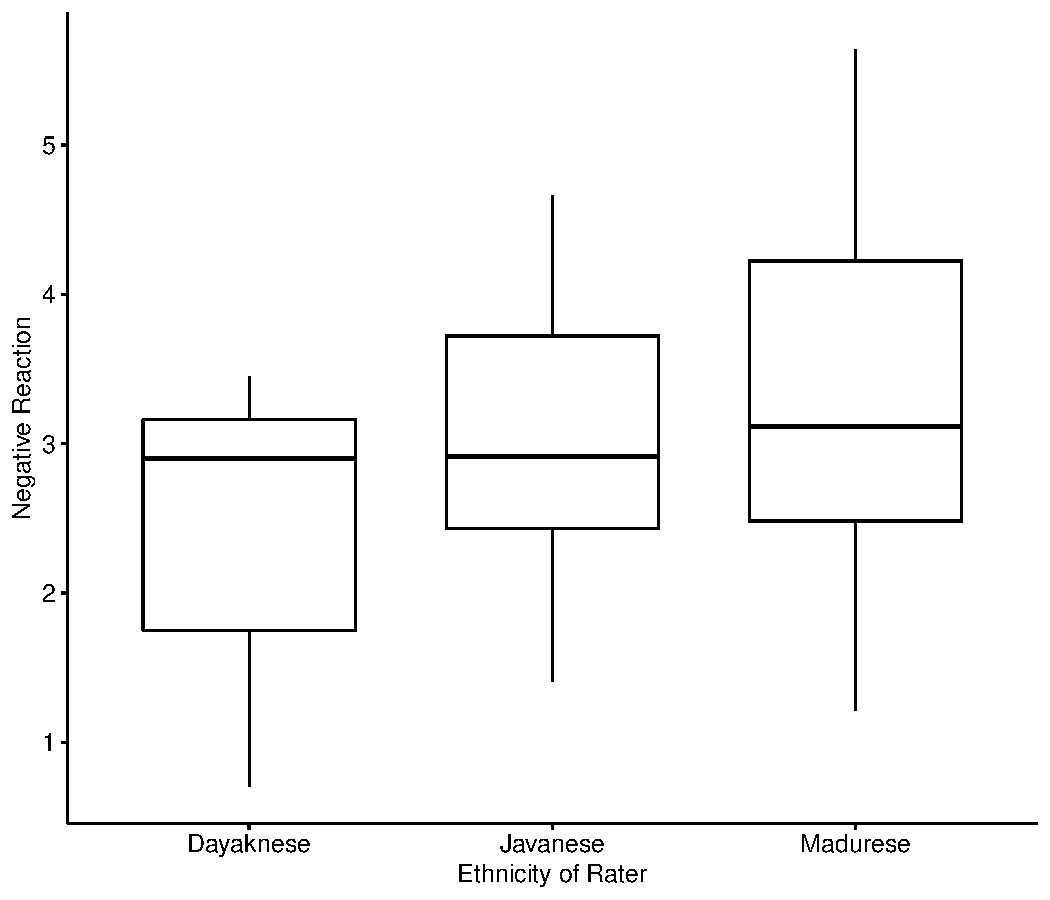
\includegraphics{ReCenterPsychStats_files/figure-latex/unnamed-chunk-174-1.pdf}

\hypertarget{my-apa-style-results-section}{%
\section{My APA Style Results Section}\label{my-apa-style-results-section}}

First, I am reluctant to term anything ``final.'' It seems like there is always the possibility or revision. Given that I demonstrated a number of options, let me first show the workflow with the particular path I took:

\begin{figure}
\centering
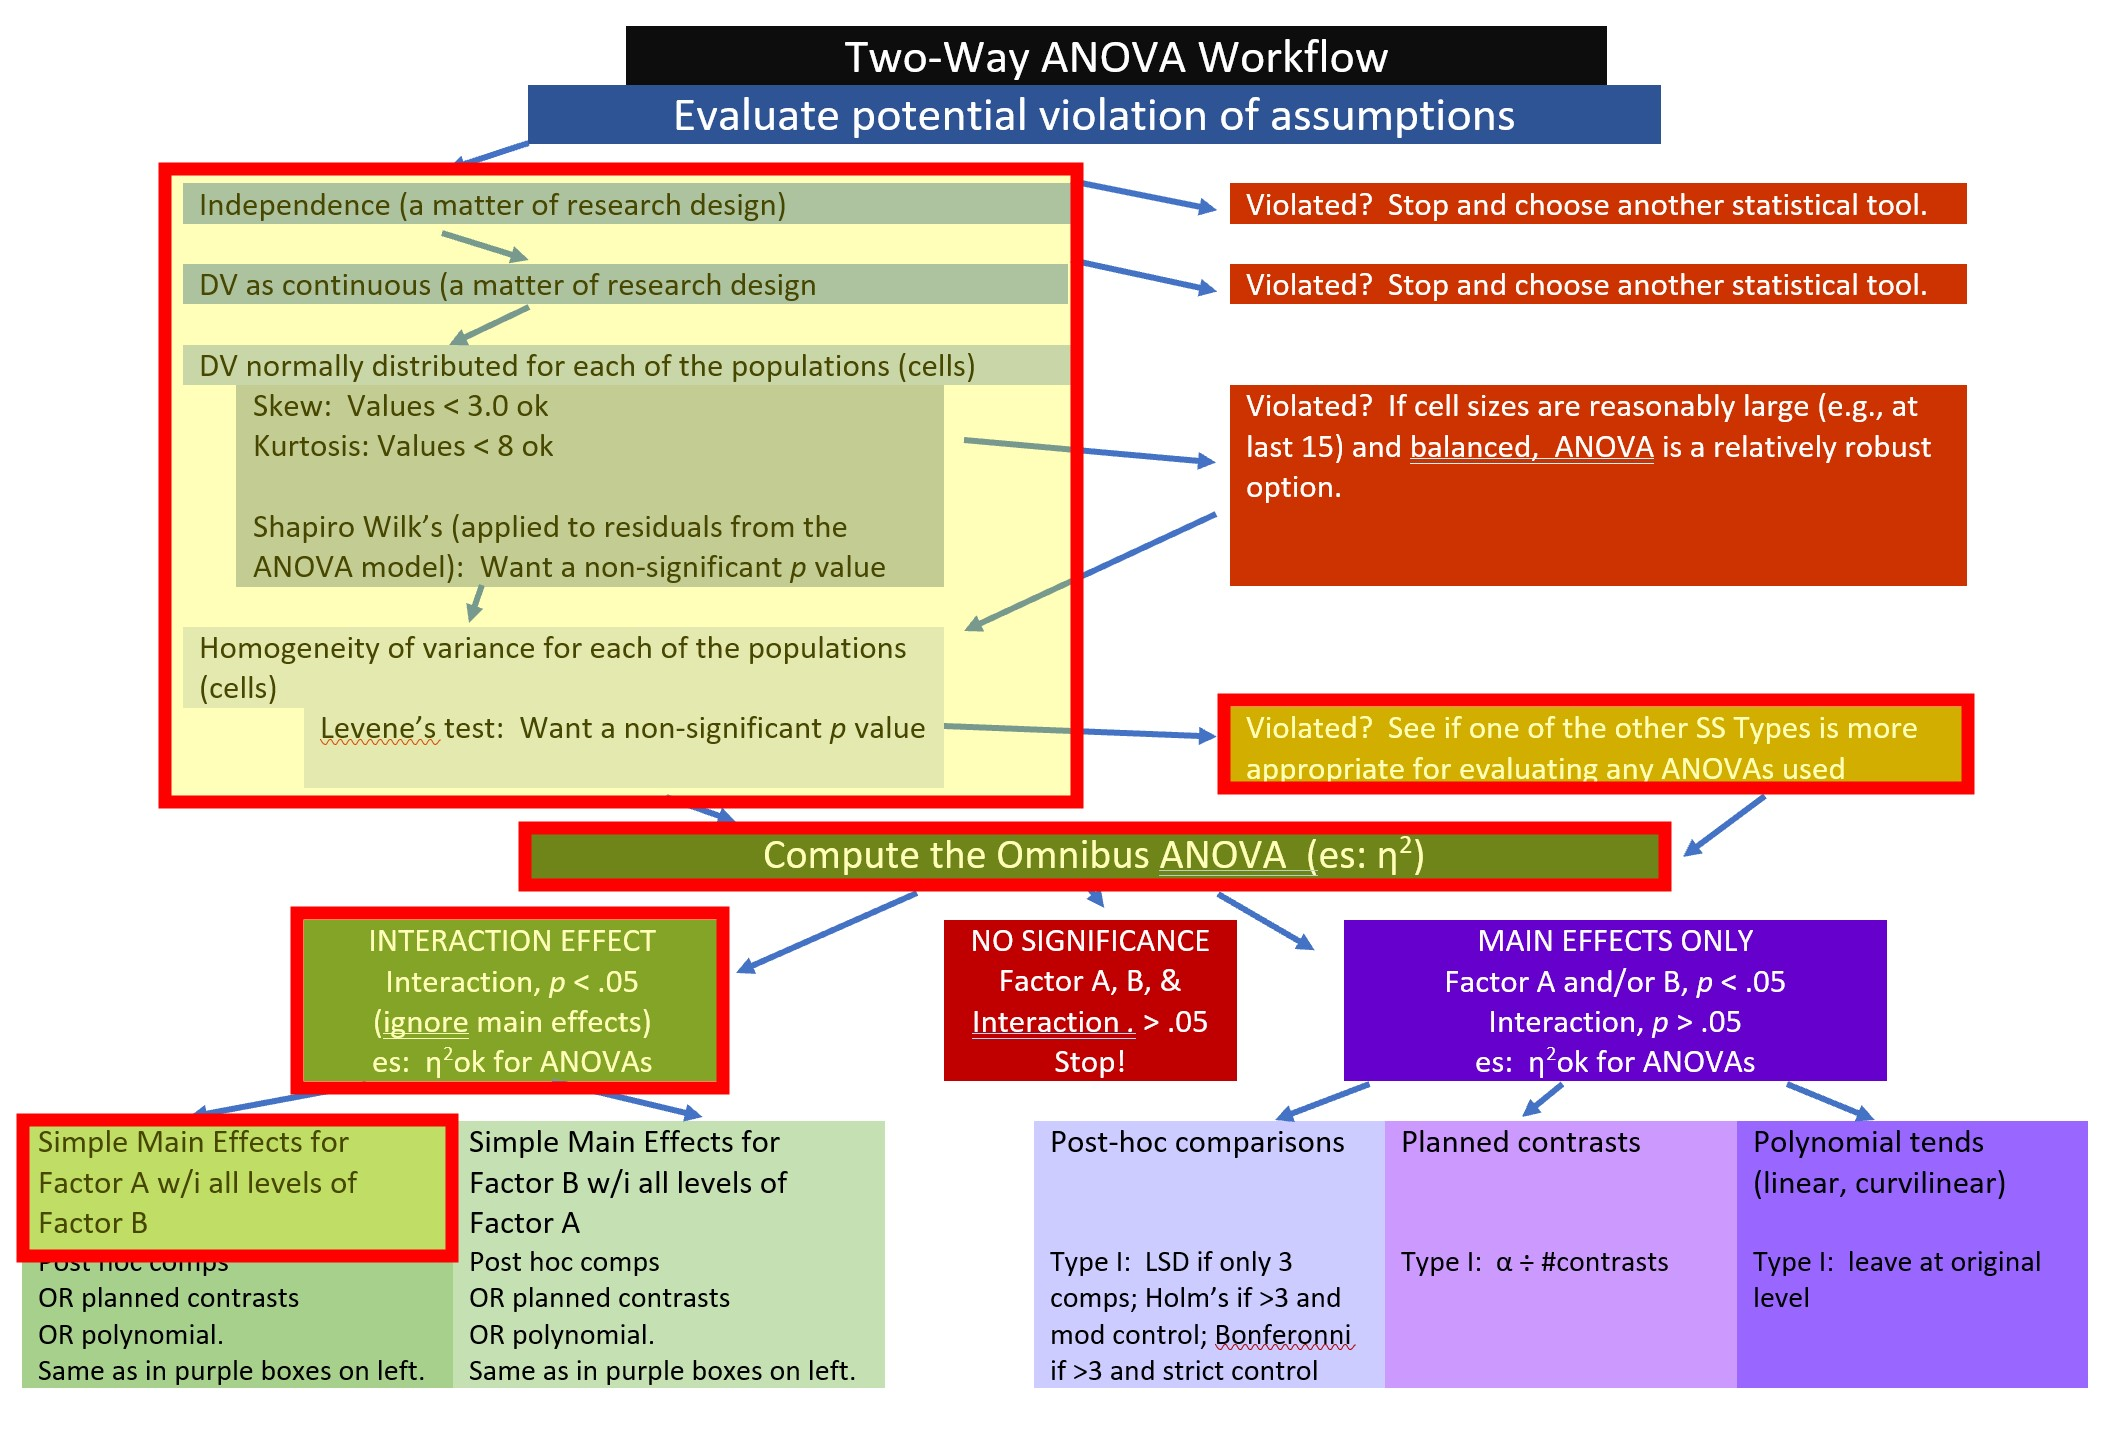
\includegraphics{images/factorial/WrkFlw_mypath.jpg}
\caption{Image our place in the Two-Way ANOVA Workflow.}
\end{figure}

In light of that, here's the final write-up:

\textbf{Results}

A 3 X 2 ANOVA was conducted to evaluate the effects of rater ethnicity (3 levels, Dayaknese, Madurese, Javanese) and photo stimulus (2 levels, Dayaknese on Madurese,) on negative reactions to the photo stimuli. Results of Levene's test for equality of error variances indicated violation of the assumption, (\(F\){[}5, 105{]} = 8.834, \(p\) \textless{} .001). Our analysis of the individual cell means (see Table 1 for means and standard deviations) suggested skew and kurtosis were within the bounds considered to be normally distributed \citep{kline_principles_2016}. A non-significant Shapiro-Wilk normality test (applied to the residuals from the factorial ANOVA model) provided further evidence that the assumption of normality was not violated (\(W\) = 0.9846, \(p\) = 0.234).

Computing sums of squares with a Type II approach, the results for the ANOVA indicated a significant main effect for ethnicity of the rater (\emph{F}{[}2, 105{]} = 8.077, \emph{p} \textless{} .001, \(\eta ^{2}\) = 0.107), a significant main effect for photo stimulus, (\emph{F}{[}1, 105{]} = 19.346, \emph{p} \textless{} .001, \(\eta ^{2}\) = 0.127), and a significant interaction effect (\emph{F}{[}2, 105{]} = 5.696, \emph{p} = .004, \(\eta ^{2}\) = 0.075).

To explore the interaction effect, we followed with a test of the simple main effect of photo stimulus within the ethnicity of the rater. That is, we looked at the effect of the photo stimulus within the Dayaknese, Madurese, and Javanese groups, separately. To control for Type I error across the three simple main effects, we set alpha at .017 (.05/3). Results indicated significant differences for Dayaknese (\emph{F} {[}1, 33{]} = 50.4, \emph{p} \textless{} .001, \(\eta ^{2}\) = 0.60.) and Javanese ethnic groups (\emph{F} {[}1, 35{]}= 17.18, \emph{p} \textless{} .001, \(\eta ^{2}\) = 0.33), but not for the Madurese ethnic group (\emph{F} {[}1, 37{]} = 0.000, \emph{p} = .993, \(\eta ^{2}\) \textless{} .001). As illustrated in Figure 1, the Dayaknese and Javanese rathers both reported stronger negative reactions to the Madurese. The differences in ratings for the Madurese were not statistically significantly different. In this way, the rater's ethnic group moderated the relationship between the photo stimulus and negative reactions.

\begin{Shaded}
\begin{Highlighting}[]
\NormalTok{ggpubr}\SpecialCharTok{::}\FunctionTok{ggboxplot}\NormalTok{(Ramdhani\_df, }\AttributeTok{x =} \StringTok{"Rater"}\NormalTok{, }\AttributeTok{y =} \StringTok{"Negative"}\NormalTok{, }\AttributeTok{color =} \StringTok{"Photo"}\NormalTok{,}
    \AttributeTok{xlab =} \StringTok{"Ethnicity of Rater"}\NormalTok{, }\AttributeTok{ylab =} \StringTok{"Negative Reaction"}\NormalTok{)}
\end{Highlighting}
\end{Shaded}

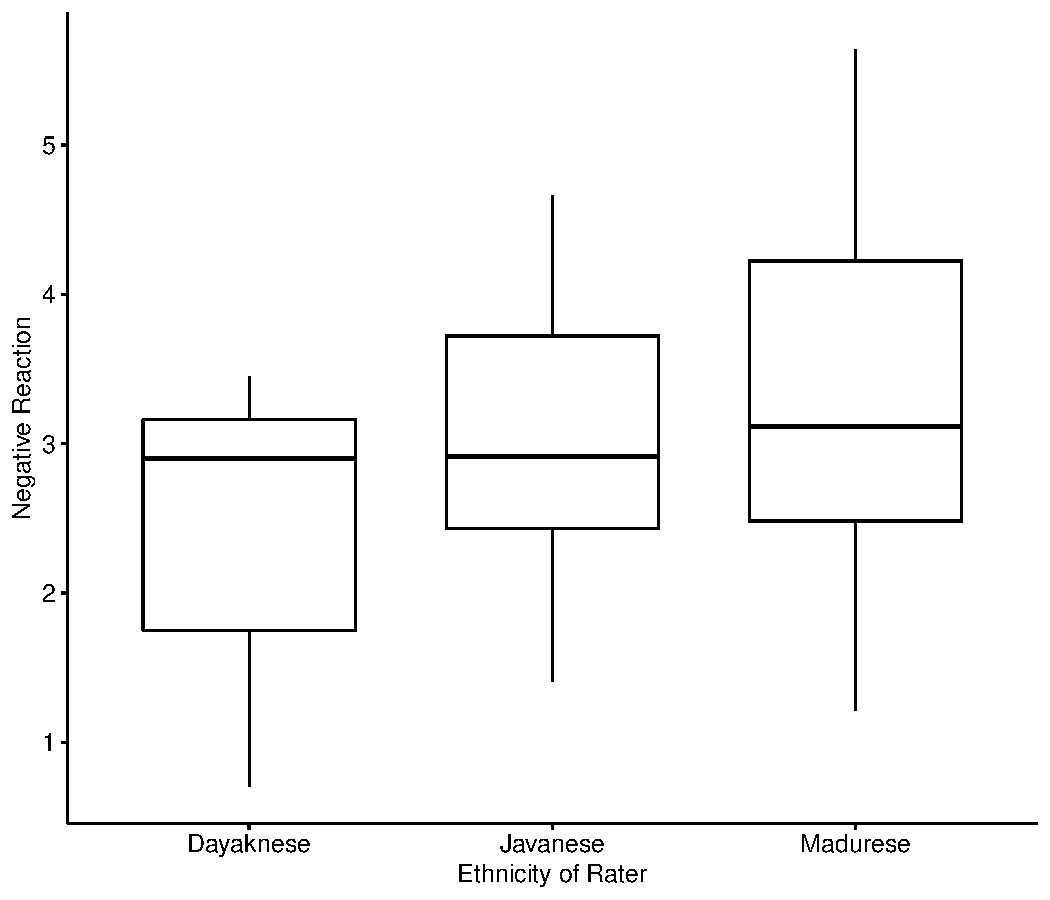
\includegraphics{ReCenterPsychStats_files/figure-latex/unnamed-chunk-175-1.pdf}

\begin{Shaded}
\begin{Highlighting}[]
\NormalTok{apaTables}\SpecialCharTok{::}\FunctionTok{apa.2way.table}\NormalTok{(}\AttributeTok{iv1 =}\NormalTok{ Rater, }\AttributeTok{iv2 =}\NormalTok{ Photo, }\AttributeTok{dv =}\NormalTok{ Negative, }\AttributeTok{data =}\NormalTok{ Ramdhani\_df,}
    \AttributeTok{landscape =} \ConstantTok{TRUE}\NormalTok{, }\AttributeTok{table.number =} \DecValTok{1}\NormalTok{, }\AttributeTok{filename =} \StringTok{"Table\_1\_MeansSDs.doc"}\NormalTok{)}
\end{Highlighting}
\end{Shaded}

\begin{verbatim}

Table 1 

Means and standard deviations for Negative as a function of a 3(Rater) X 2(Photo) design 

               Photo                   
           Dayaknese      Madurese     
     Rater         M   SD        M   SD
 Dayaknese      1.82 0.77     3.13 0.16
  Javanese      2.52 0.74     3.46 0.64
  Madurese      3.30 1.03     3.30 1.33

Note. M and SD represent mean and standard deviation, respectively. 
\end{verbatim}

\begin{Shaded}
\begin{Highlighting}[]
\NormalTok{apaTables}\SpecialCharTok{::}\FunctionTok{apa.aov.table}\NormalTok{(TwoWay\_neg, }\AttributeTok{filename =} \StringTok{"Table\_2\_effects.doc"}\NormalTok{,}
    \AttributeTok{table.number =} \DecValTok{2}\NormalTok{, }\AttributeTok{type =} \StringTok{"II"}\NormalTok{)}
\end{Highlighting}
\end{Shaded}

\begin{verbatim}

Table 2 

ANOVA results using Negative as the dependent variable
 

     Predictor    SS  df    MS     F    p partial_eta2 CI_90_partial_eta2
         Rater 12.24   2  6.12  8.10 .001          .13                   
         Photo 14.62   1 14.62 19.35 .000          .16         [.06, .26]
 Rater x Photo  8.61   2  4.30  5.70 .004          .10         [.02, .18]
         Error 79.34 105  0.76                                           

Note: Values in square brackets indicate the bounds of the 90% confidence interval for partial eta-squared 
\end{verbatim}

\hypertarget{comparing-our-results-to-rhamdani-et-al.--ramdhani_affective_2018}{%
\subsection{\texorpdfstring{Comparing Our Results to Rhamdani et al. \citeyearpar{ramdhani_affective_2018}}{Comparing Our Results to Rhamdani et al. {[}-@ramdhani\_affective\_2018{]}}}\label{comparing-our-results-to-rhamdani-et-al.--ramdhani_affective_2018}}

As is common in simulations, our results approximate the findings reported in the manuscript, but does not replicate them exactly. Our main and interaction effects map on very closely. However, in the follow-up tests, while our findings that Dayaknese rated the Madurese photos more negatively, the findings related to the Javanese' and Madurese' ratings wiggled around some. A close look at the figures can explain that with varying variability and means with similar values, this is probable. I find it to be a useful lesson in ``what it takes'' to get stable, meaningful results.

\hypertarget{options-for-assumption-violations}{%
\section{Options for Assumption Violations}\label{options-for-assumption-violations}}

In one-way ANOVA we could simply apply the Welch's alternative. It's not so easy in factorial ANOVA. One alternative, though, is to change the sums of squares type used in the ANOVA calculations.

In ANOVA models sums of squares can be calculated four different ways: Type I, II, III, and IV. This matters.

SS Type II is the \emph{aov()} default. It may be a best practice to go ahead and specify the SS Type in both the \emph{aov()}, eta-squared, and apaTables script so that they are consistent.

\textbf{Type I} sums of squares is similar to hierarchical linear regression in that the first predictor in the model claims as much variance as it can and the leftovers are claimed by the variable entered next -- each claiming as much as possible leaving the leftovers for what follows. Unless the variables are completely independent of each other (unlikely), Type I sums of squares cannot evaluate the true main effect of each variable. Type I should not be used to evaluate main effects and interactions because the order of predictors will affect the results.

\textbf{Type II} (the R default) is appropriate if you are interested main effects because it ignores the effect of any interactions involving the main effect. Thus, variance from a main effect is not ``lost'' to any interaction terms containing that effect. Type II is appropriate for main effects analyses only, but should not be used when evaluating interaction effects. Type II sums of squares is not affected by the type of contrast coding used to specify the predictor variables.

\textbf{Type III} is the default in many stats packages -- but not R. In Type III all effects (main effects and interactions) are evaluated (simultaneously) taking into consideration all other effects in the model (not just the ones entered before). Type III is more robust to unequal samples sizes (e.g., unbalanced designs). Type III is best when predictors are encoded with orthogonal contrasts.

*\textbf{Type IV} is identical to Type III except it requires no missing cells.

Field \citeyearpar{field_discovering_2012} suggested that it is safest to stick with Type III sums of squares. We apply the type to the model we create in the initial run. For more information, check out this explanation on \href{https://www.r-bloggers.com/2011/03/anova-\%E2\%80\%93-type-iiiiii-ss-explained/}{r-bloggers}.

Many researchers automatically use Type III as the SS type. Today I went with the R default because

\begin{itemize}
\tightlist
\item
  Type II sums of squares was used in hand-calculations,
\item
  Our example was reasonably balanced (equal cell sizes), and
\item
  We had only violated the homogeneity of variance assumption.
\end{itemize}

For demonstration purposes, let's run the Type III alternative to see the differences:

\begin{Shaded}
\begin{Highlighting}[]
\CommentTok{\# this is what we did}
\NormalTok{car}\SpecialCharTok{::}\FunctionTok{Anova}\NormalTok{(TwoWay\_neg)}
\end{Highlighting}
\end{Shaded}

\begin{verbatim}
Anova Table (Type II tests)

Response: Negative
            Sum Sq  Df F value     Pr(>F)    
Rater       12.238   2  8.0977  0.0005363 ***
Photo       14.619   1 19.3462 0.00002623 ***
Rater:Photo  8.609   2  5.6964  0.0044803 ** 
Residuals   79.341 105                       
---
Signif. codes:  0 '***' 0.001 '**' 0.01 '*' 0.05 '.' 0.1 ' ' 1
\end{verbatim}

\begin{Shaded}
\begin{Highlighting}[]
\CommentTok{\# We change the SS type by applying it to our model.}
\NormalTok{car}\SpecialCharTok{::}\FunctionTok{Anova}\NormalTok{(TwoWay\_neg, }\AttributeTok{type =} \StringTok{"III"}\NormalTok{)}
\end{Highlighting}
\end{Shaded}

\begin{verbatim}
Anova Table (Type III tests)

Response: Negative
            Sum Sq  Df F value              Pr(>F)    
(Intercept) 56.173   1 74.3388 0.00000000000007422 ***
Rater       19.805   2 13.1051 0.00000830116650983 ***
Photo       15.040   1 19.9034 0.00002051829053731 ***
Rater:Photo  8.609   2  5.6964             0.00448 ** 
Residuals   79.341 105                                
---
Signif. codes:  0 '***' 0.001 '**' 0.01 '*' 0.05 '.' 0.1 ' ' 1
\end{verbatim}

Note that the sums of squares are somewhat different between models -- and that the Type III tests includes an intercept. In today's example, the statistical significance remains the same across the models.

Now let's compare the effect sizes across models.

\begin{Shaded}
\begin{Highlighting}[]
\NormalTok{lsr}\SpecialCharTok{::}\FunctionTok{etaSquared}\NormalTok{(TwoWay\_neg)}
\end{Highlighting}
\end{Shaded}

\begin{verbatim}
                eta.sq eta.sq.part
Rater       0.10662441  0.13363091
Photo       0.12736755  0.15558329
Rater:Photo 0.07500609  0.09788289
\end{verbatim}

\begin{Shaded}
\begin{Highlighting}[]
\NormalTok{lsr}\SpecialCharTok{::}\FunctionTok{etaSquared}\NormalTok{(TwoWay\_neg, }\AttributeTok{type =} \DecValTok{3}\NormalTok{)}
\end{Highlighting}
\end{Shaded}

\begin{verbatim}
                eta.sq eta.sq.part
Rater       0.17255745  0.19975734
Photo       0.13103575  0.15935009
Rater:Photo 0.07500609  0.09788289
\end{verbatim}

The Type III effect size for Rater is higher; the others are quite similar.

\hypertarget{power}{%
\section{Power}\label{power}}

Asking about \emph{power} can be a euphemistic way of asking, ``How large should my sample size be?''

Power is defined as the ability of the test to detect statistical significance when there is such. It's represented formulaically as (1 - \emph{P})(Type II error). Power is traditionally set at 80\% (or .8)

We will do both -- evaluate the power of our current example and then work backwards to estimate the sample size needed (which is our usual question for MRPs and dissertations).

We'll use the \emph{pwr.2way()} function from the \emph{pwr2} package.
Helpful resources are found here:

\begin{itemize}
\tightlist
\item
  \url{https://cran.r-project.org/web/packages/pwr2/pwr2.pdf}
\item
  \url{https://rdrr.io/cran/pwr2/man/ss.2way.html}
\end{itemize}

The \emph{pwr.2way()} and \emph{ss.2way()} functions require the following:

\begin{itemize}
\tightlist
\item
  \textbf{a} number of groups in Factor A
\item
  \textbf{b} number of groups in Factor B
\item
  \textbf{alpha} significant level (Type I error probaility)
\item
  \textbf{beta} Type II error probability (Power = 1 - beta; traditionally set at .1 or .2)
\item
  \textbf{f.A} the \emph{f} effect size of Factor A
\item
  \textbf{f.B} the \emph{f} effect size of Factor B
\item
  \textbf{B} Iteration times, default is 100
\end{itemize}

Hints for calculating the \emph{f.A} and \emph{f.B} values:

\begin{itemize}
\tightlist
\item
  In this case, we will rerun the statistic, grab both effect sizes, and convert them to the \emph{f} (not the \(f^2\))

  \begin{itemize}
  \tightlist
  \item
    calculation can be straightforward, either use an online calculator, a hand-calculated formula, or the \emph{eta2\_to\_f} function from the \emph{effectsize}
  \end{itemize}
\item
  When an effect size is unknown, you can substitute what you expect using Cohen's guidelines of .10, .25, and .40 as small, medium, and large (for the \emph{f}, not \(F^2\))
\end{itemize}

Let's quickly rerun our model to get both the df and calculate the \emph{f} effect value

\begin{Shaded}
\begin{Highlighting}[]
\NormalTok{lsr}\SpecialCharTok{::}\FunctionTok{etaSquared}\NormalTok{(TwoWay\_neg, }\AttributeTok{anova =} \ConstantTok{TRUE}\NormalTok{)}
\end{Highlighting}
\end{Shaded}

\begin{verbatim}
                eta.sq eta.sq.part        SS  df         MS         F
Rater       0.10662441  0.13363091 12.237770   2  6.1188848  8.097730
Photo       0.12736755  0.15558329 14.618555   1 14.6185546 19.346190
Rater:Photo 0.07500609  0.09788289  8.608791   2  4.3043955  5.696435
Residuals   0.69127788          NA 79.341113 105  0.7556296        NA
                        p
Rater       0.00053629628
Photo       0.00002622821
Rater:Photo 0.00448026007
Residuals              NA
\end{verbatim}

\begin{Shaded}
\begin{Highlighting}[]
\CommentTok{\# get the partial eta{-}square (second number) and dfs}
\end{Highlighting}
\end{Shaded}

If we want to understand power in our analysis, we need to convert our effect size for the \emph{interaction} to \(f\) effect size (this is not the same as the \emph{F} test). The \emph{effectsize} package has a series of converters. We can use the \emph{eta2\_to\_f()} function.

\begin{Shaded}
\begin{Highlighting}[]
\NormalTok{effectsize}\SpecialCharTok{::}\FunctionTok{eta2\_to\_f}\NormalTok{(}\FloatTok{0.1066}\NormalTok{)  }\CommentTok{\#FactorA {-}{-} Rater}
\end{Highlighting}
\end{Shaded}

\begin{verbatim}
[1] 0.3454265
\end{verbatim}

\begin{Shaded}
\begin{Highlighting}[]
\NormalTok{effectsize}\SpecialCharTok{::}\FunctionTok{eta2\_to\_f}\NormalTok{(}\FloatTok{0.1274}\NormalTok{)  }\CommentTok{\#Factor B {-}{-} Photo}
\end{Highlighting}
\end{Shaded}

\begin{verbatim}
[1] 0.3821001
\end{verbatim}

\hypertarget{post-hoc-power-analysis}{%
\subsection{Post Hoc Power Analysis}\label{post-hoc-power-analysis}}

Now we calculate power for our existing model. We'll use the package \emph{pwr2} and the function \emph{pwr.2way()}. To specify this we identify:

\begin{itemize}
\tightlist
\item
  a: number of groups for Factor A (Rater)
\item
  b: number of groups for Factor B (Photo)
\item
  size.A: sample size per group in Factor A (because ours differ slightly, I divided the N by the number of groups)
\item
  size.B: sample size per group in Factor B (because ours differ slightly, I divided the N by the number of groups)
\item
  f.A: Effect size of Factor A
\item
  f.A.: Effect size of Factor B
\end{itemize}

\begin{Shaded}
\begin{Highlighting}[]
\NormalTok{pwr2}\SpecialCharTok{::}\FunctionTok{pwr.2way}\NormalTok{(}\AttributeTok{a =} \DecValTok{3}\NormalTok{, }\AttributeTok{b =} \DecValTok{2}\NormalTok{, }\AttributeTok{alpha =} \FloatTok{0.05}\NormalTok{, }\AttributeTok{size.A =} \DecValTok{37}\NormalTok{, }\AttributeTok{size.B =} \DecValTok{55}\NormalTok{, }\AttributeTok{f.A =} \FloatTok{0.345}\NormalTok{,}
    \AttributeTok{f.B =} \FloatTok{0.382}\NormalTok{)}
\end{Highlighting}
\end{Shaded}

\begin{verbatim}
     Balanced two-way analysis of variance power calculation 

              a = 3
              b = 2
            n.A = 37
            n.B = 55
      sig.level = 0.05
        power.A = 0.9974259
        power.B = 0.9999996
          power = 0.9974259

NOTE: power is the minimum power among two factors
\end{verbatim}

At 0.997 (Rater), 0.999 (Photo), and 0.997 (interaction), our power to detect a significant effect for Factor A/Rater and Factor B/Photo was huge!

\hypertarget{estimating-sample-size-requirements}{%
\subsection{Estimating Sample Size Requirements}\label{estimating-sample-size-requirements}}

If we want to replicate this study we could use its results to estimate what would be needed for the replication.

In this specification:

\begin{itemize}
\tightlist
\item
  a: number of groups for Factor A (Rater)
\item
  b: number of groups for Factor B (Photo)
\item
  alpha: significance level (Type I error probability); usually .05
\item
  beta: Type II error probability (Power = 1-beta); usually .80
\item
  f.A: Effect size (\emph{f}) of Factor A (this time we know; other times we can guess from previously published literature)
\item
  f.A.: Effect size (\emph{f}) of Factor B
\item
  B: iteration times, default number is 100
\end{itemize}

\begin{Shaded}
\begin{Highlighting}[]
\NormalTok{pwr2}\SpecialCharTok{::}\FunctionTok{ss.2way}\NormalTok{(}\AttributeTok{a =} \DecValTok{3}\NormalTok{, }\AttributeTok{b =} \DecValTok{2}\NormalTok{, }\AttributeTok{alpha =} \FloatTok{0.05}\NormalTok{, }\AttributeTok{beta =} \FloatTok{0.8}\NormalTok{, }\AttributeTok{f.A =} \FloatTok{0.345}\NormalTok{, }\AttributeTok{f.B =} \FloatTok{0.382}\NormalTok{,}
    \AttributeTok{B =} \DecValTok{100}\NormalTok{)}
\end{Highlighting}
\end{Shaded}

\begin{verbatim}
     Balanced two-way analysis of variance sample size adjustment 

              a = 3
              b = 2
      sig.level = 0.05
          power = 0.2
              n = 3

NOTE: n is number in each group, total sample = 18
\end{verbatim}

Curiously, that's just about the number that was in each of the six cells!

Often times researchers will play around with the \emph{f} values. Remember Cohen's indication of small (.10), medium (.25), and large (.40). Let's see what happens when we enter different values. Specifically, what if we only had a medium effect?

\begin{Shaded}
\begin{Highlighting}[]
\NormalTok{pwr2}\SpecialCharTok{::}\FunctionTok{ss.2way}\NormalTok{(}\AttributeTok{a =} \DecValTok{3}\NormalTok{, }\AttributeTok{b =} \DecValTok{2}\NormalTok{, }\AttributeTok{alpha =} \FloatTok{0.05}\NormalTok{, }\AttributeTok{beta =} \FloatTok{0.8}\NormalTok{, }\AttributeTok{f.A =} \FloatTok{0.25}\NormalTok{, }\AttributeTok{f.B =} \FloatTok{0.25}\NormalTok{,}
    \AttributeTok{B =} \DecValTok{100}\NormalTok{)  }\CommentTok{\#if we expected a medium effect}
\end{Highlighting}
\end{Shaded}

\begin{verbatim}
     Balanced two-way analysis of variance sample size adjustment 

              a = 3
              b = 2
      sig.level = 0.05
          power = 0.2
              n = 6

NOTE: n is number in each group, total sample = 36
\end{verbatim}

And what would happen if we only had a small effect?

\begin{Shaded}
\begin{Highlighting}[]
\NormalTok{pwr2}\SpecialCharTok{::}\FunctionTok{ss.2way}\NormalTok{(}\AttributeTok{a =} \DecValTok{3}\NormalTok{, }\AttributeTok{b =} \DecValTok{2}\NormalTok{, }\AttributeTok{alpha =} \FloatTok{0.05}\NormalTok{, }\AttributeTok{beta =} \FloatTok{0.8}\NormalTok{, }\AttributeTok{f.A =} \FloatTok{0.1}\NormalTok{, }\AttributeTok{f.B =} \FloatTok{0.1}\NormalTok{,}
    \AttributeTok{B =} \DecValTok{100}\NormalTok{)  }\CommentTok{\#if we expected a small effect}
\end{Highlighting}
\end{Shaded}

\begin{verbatim}
     Balanced two-way analysis of variance sample size adjustment 

              a = 3
              b = 2
      sig.level = 0.05
          power = 0.2
              n = 30

NOTE: n is number in each group, total sample = 180
\end{verbatim}

\hypertarget{practice-problems-2}{%
\section{Practice Problems}\label{practice-problems-2}}

In each of these lessons I provide suggestions for practice that allow you to select one or more problems that offer differing levels of difficulty. Whichever you choose, you will focus on these larger steps in factorial-way ANOVA, including:

\begin{itemize}
\tightlist
\item
  test the statistical assumptions
\item
  conduct a two-way ANOVA, including

  \begin{itemize}
  \tightlist
  \item
    omnibus test and effect size
  \item
    report main and interaction effects
  \item
    conduct follow-up testing of simple main effects
  \end{itemize}
\item
  write a results section to include a figure and tables
\end{itemize}

\hypertarget{problem-1-play-around-with-this-simulation.-1}{%
\subsection{Problem \#1: Play around with this simulation.}\label{problem-1-play-around-with-this-simulation.-1}}

Copy the script for the simulation and then change (at least) one thing in the simulation to see how it impacts the results.

\begin{itemize}
\tightlist
\item
  If two-way ANOVA is new to you, perhaps you just change the number in ``set.seed(210731)'' from 210731 to something else. Your results should parallel those obtained in the lecture, making it easier for you to check your work as you go.
\item
  If you are interested in power, change the sample size to something larger or smaller.
\item
  If you are interested in variability (i.e., the homogeneity of variance assumption), perhaps you change the standard deviations in a way that violates the assumption.
\end{itemize}

\hypertarget{problem-2-conduct-a-factorial-anova-with-the-positive-evaluation-dependent-variable.}{%
\subsection{\texorpdfstring{Problem \#2: Conduct a factorial ANOVA with the \emph{positive evaluation} dependent variable.}{Problem \#2: Conduct a factorial ANOVA with the positive evaluation dependent variable.}}\label{problem-2-conduct-a-factorial-anova-with-the-positive-evaluation-dependent-variable.}}

The Ramdhani et al. \citeyearpar{ramdhani_affective_2018} article has two dependent variables (negative and positive evaluation). Each is suitable for two-way ANOVA. I used \emph{negative evaluation} as the dependent variable; you are welcome to conduct the analysis with \emph{positive evaluation} as the dependent variable.

\hypertarget{problem-3-try-something-entirely-new.-1}{%
\subsection{Problem \#3: Try something entirely new.}\label{problem-3-try-something-entirely-new.-1}}

Using data for which you have permission and access (e.g., IRB approved data you have collected or from your lab; data you simulate from a published article; data from an open science repository; data from other chapters in this OER), complete a two-way, factorial ANOVA. Please have at least 3 levels for one predictor and at least 2 levels for the second predictor.

\hypertarget{grading-rubric-2}{%
\subsection{Grading Rubric}\label{grading-rubric-2}}

Regardless which option(s) you chose, use the elements in the grading rubric to guide you through the practice.

\begin{longtable}[]{@{}
  >{\raggedright\arraybackslash}p{(\columnwidth - 4\tabcolsep) * \real{0.5493}}
  >{\centering\arraybackslash}p{(\columnwidth - 4\tabcolsep) * \real{0.2535}}
  >{\centering\arraybackslash}p{(\columnwidth - 4\tabcolsep) * \real{0.1972}}@{}}
\toprule
\begin{minipage}[b]{\linewidth}\raggedright
Assignment Component
\end{minipage} & \begin{minipage}[b]{\linewidth}\centering
Points Possible
\end{minipage} & \begin{minipage}[b]{\linewidth}\centering
Points Earned
\end{minipage} \\
\midrule
\endhead
1. Narrate the research vignette, describing the IV and DV & 5 & \_\_\_\_\_ \\
2. Simulate (or import) and format data & 5 & \_\_\_\_\_ \\
3. Evaluate statistical assumptions & 5 & \_\_\_\_\_ \\
4. Conduct omnibus ANOVA (w effect size) & 5 & \_\_\_\_\_ \\
5. Conduct one set of follow-up tests; narrate your choice & 5 & \_\_\_\_\_ \\
6. Describe approach for managing Type I error & 5 & \_\_\_\_\_ \\
7. APA style results with table(s) and figure & 5 & \_\_\_\_\_ \\
8 Explanation to grader & 5 & \_\_\_\_\_ \\
\textbf{Totals} & 40 & \_\_\_\_\_ \\
\bottomrule
\end{longtable}

\hypertarget{Repeated}{%
\chapter{One-Way Repeated Measures ANOVA}\label{Repeated}}

\href{https://spu.hosted.panopto.com/Panopto/Pages/Viewer.aspx?pid=c8f5737f-d00d-4fa4-ba3c-ad8b01762258}{Screencasted Lecture Link}

In the prior lessons, a critical assumption is that the observations must be ``independent.'' That is, related people (partners, parent/child, manager/employee) cannot comprise the data and there cannot be multiple waves of data for the same person. Repeated measures ANOVA is created specifically for this \emph{dependent} purpose. This lessons focuses on the one-way repeated measures ANOVA, where we measure changes across time.

\hypertarget{navigating-this-lesson-4}{%
\section{Navigating this Lesson}\label{navigating-this-lesson-4}}

There is just over one hour of lecture. If you work through the materials with me plan for an additional two hours

While the majority of R objects and data you will need are created within the R script that sources the chapter, occasionally there are some that cannot be created from within the R framework. Additionally, sometimes links fail. All original materials are provided at the \href{https://github.com/lhbikos/ReCenterPsychStats}{Github site} that hosts the book. More detailed guidelines for ways to access all these materials are provided in the OER's \protect\hyperlink{ReCintro}{introduction}

\hypertarget{learning-objectives-4}{%
\subsection{Learning Objectives}\label{learning-objectives-4}}

Learning objectives from this lecture include the following:

\begin{itemize}
\tightlist
\item
  Evaluate the suitability of a research design/question and dataset for conducting a one-way repeated measures ANOVA; identify alternatives if the data is not suitable.
\item
  Hand-calculate a one-way repeated measures ANOVAs

  \begin{itemize}
  \tightlist
  \item
    describing the partitioning of variance as it relates to model/residual; within/between.
  \end{itemize}
\item
  Test the assumptions for one-way repeated measures ANOVA.
\item
  Conduct a one-way repeated measures ANOVA (omnibus and follow-up) in R.
\item
  Interpret output from the one-way repeated measures ANOVA (and follow-up).
\item
  Prepare an APA style results section of the one-way repeated measures ANOVA output.
\item
  Demonstrate how an increased sample size increases the power of a statistical test.
\end{itemize}

\hypertarget{planning-for-practice-3}{%
\subsection{Planning for Practice}\label{planning-for-practice-3}}

The suggestions for homework are graded in complexity with more complete descriptions at the end of the chapter follow these suggestions.

\begin{itemize}
\tightlist
\item
  Rework the problem in the chapter by changing the random seed in the code that simulates the data. This should provide minor changes to the data, but the results will likely be very similar.
\item
  There were no additional variables in this example. However, you'll see we do have an issue with statistical power. Perhaps change the sample size to see if it changes (maybe stabilizes?) the results.
\item
  Conduct a one-way repeated measures ANOVA with data to which you have access. This could include data you simulate on your own or from a published article.
\end{itemize}

\hypertarget{readings-resources-3}{%
\subsection{Readings \& Resources}\label{readings-resources-3}}

In preparing this chapter, I drew heavily from the following resource(s). Other resources are cited (when possible, linked) in the text with complete citations in the reference list.

\begin{itemize}
\tightlist
\item
  \emph{Repeated Measures ANOVA in R: The Ultimate Guide}. (n.d.). Datanovia. Retrieved October 19, 2020, from \url{https://www.datanovia.com/en/lessons/repeated-measures-anova-in-r}

  \begin{itemize}
  \tightlist
  \item
    This website is an excellent guide for both one-way repeated measures and mixed design ANOVA. A great resource for both the conceptual and procedural. This is the guide I have used for the basis of the lecture. Working through their example would be great additional practice.
  \end{itemize}
\item
  Green, S. B., \& Salkind, N. J. (2014). One-Way Repeated Measures Analysis of Variance (Lesson 29). In \emph{Using SPSS for Windows and Macintosh: Analyzing and understanding data} (Seventh edition., pp.~209--217). Pearson.

  \begin{itemize}
  \tightlist
  \item
    For years I taught from the Green and Salkind text. Even though it was written for SPSS, the authors do a terrific job of walking the reader through the one-way repeated measures logic and process.
  \end{itemize}
\item
  Amodeo, A. L., Picariello, S., Valerio, P., \& Scandurra, C. (2018). Empowering transgender youths: Promoting resilience through a group training program. \emph{Journal of Gay \& Lesbian Mental Health, 22}(1), 3--19.

  \begin{itemize}
  \tightlist
  \item
    This mixed methods (qualitative and quantitative) includes a one-way repeated measures example.
  \end{itemize}
\end{itemize}

\hypertarget{packages-2}{%
\subsection{Packages}\label{packages-2}}

The packages used in this lesson are embedded in this code. When the hashtags are removed, the script below will (a) check to see if the following packages are installed on your computer and, if not (b) install them.

\begin{Shaded}
\begin{Highlighting}[]
\CommentTok{\# will install the package if not already installed}
\CommentTok{\# if(!require(knitr))\{install.packages(\textquotesingle{}knitr\textquotesingle{})\}}
\CommentTok{\# if(!require(tidyverse))\{install.packages(\textquotesingle{}tidyverse\textquotesingle{})\} \#manipulate}
\CommentTok{\# data if(!require(psych))\{install.packages(\textquotesingle{}psych\textquotesingle{})\}}
\CommentTok{\# if(!require(ggpubr))\{install.packages(\textquotesingle{}ggpubr\textquotesingle{})\} \#easy plots}
\CommentTok{\# if(!require(rstatix))\{install.packages(\textquotesingle{}rstatix\textquotesingle{})\} \#pipe{-}friendly R}
\CommentTok{\# functions if(!require(data.table))\{install.packages(\textquotesingle{}data.table\textquotesingle{})\}}
\CommentTok{\# \#pipe{-}friendly R functions}
\CommentTok{\# if(!require(reshape2))\{install.packages(\textquotesingle{}reshape2\textquotesingle{})\} \#pipe{-}friendly}
\CommentTok{\# R functions}
\CommentTok{\# if(!require(effectsize))\{install.packages(\textquotesingle{}effectsize\textquotesingle{})\} \#converts}
\CommentTok{\# effect sizes for use in power analysis}
\CommentTok{\# if(!require(WebPower))\{install.packages(\textquotesingle{}WebPower\textquotesingle{})\} \#power}
\CommentTok{\# analysis tools for repeated measures}
\CommentTok{\# if(!require(MASS))\{install.packages(\textquotesingle{}MASS\textquotesingle{})\} \#power analysis tools}
\CommentTok{\# for repeated measures}
\end{Highlighting}
\end{Shaded}

\hypertarget{introducing-one-way-repeated-measures-anova}{%
\section{Introducing One-way Repeated Measures ANOVA}\label{introducing-one-way-repeated-measures-anova}}

There are a couple of typical use cases for one-way repeated measures ANOVA. In the first, the research participant is assessed in multiple conditions -- with no interested in change-over-time.

An example of a research design using this approach occurred in the Green and Salkind \citeyearpar{green_using_2014} statistics text, the one-way repeated measures vignette compared teachers' perception of stress when responding to parents, teachers, and school administrators.

\begin{figure}
\centering
\includegraphics{images/oneway_repeated/repeated_conditions.jpg}
\caption{Illustration of a research design appropriate for one-way repeated measures ANOVA}
\end{figure}

Another common use case is about time. The classic design is a pre-test, an intervention, a post-test, and a follow up. In designs like these researchers often hope that there is a positive change from pre-to-post and that that change either stays constant (from post-to-follow-up) or, perhaps, increases even further. The research vignette for this lesson is interested in change-over-time.

\begin{figure}
\centering
\includegraphics{images/oneway_repeated/repeated_design.jpg}
\caption{Illustration of a research design appropriate for one-way repeated measures ANOVA}
\end{figure}

\hypertarget{workflow-for-oneway-repeated-measures-anova}{%
\subsection{Workflow for Oneway Repeated Measures ANOVA}\label{workflow-for-oneway-repeated-measures-anova}}

The following is a proposed workflow for conducting a one-way repeated measures ANOVA.

\begin{figure}
\centering
\includegraphics{images/oneway_repeated/wf_repeated.jpg}
\caption{Image of a workflow for the one-way repeated measures ANOVA}
\end{figure}

Steps involved in analyzing the data include:

\begin{enumerate}
\def\labelenumi{\arabic{enumi}.}
\tightlist
\item
  Preparing and importing the data.
\item
  Exploring the data

  \begin{itemize}
  \tightlist
  \item
    graphs
  \item
    descriptive statistics
  \end{itemize}
\item
  Checking distributional assumptions

  \begin{itemize}
  \tightlist
  \item
    assessing normality via skew, kurtosis, Shapiro Wilks
  \item
    checking or violation of the \emph{sphericity} assumption with Mauchly's test; if violated interpret the corrected output or use a multivariate approach for the analysis
  \end{itemize}
\item
  Computing the omnibus ANOVA
\item
  Computing post-hoc comparisons, planned contrasts, or polynomial trends
\item
  Managing Type I error
\item
  Sample size/power analysis (which you should think about first -- but in the context of teaching ANOVA, it's more pedagogically sensible, here)
\end{enumerate}

\hypertarget{research-vignette-3}{%
\section{Research Vignette}\label{research-vignette-3}}

Amodeo \citep{amodeo_empowering_2018} and colleagues conducted a mixed methods study (qualitative and quantitative) to evaluate the effectiveness of an empowerment, peer-group-based, intervention with participants (\emph{N} = 8) who experienced transphobic episodes. Focus groups used qualitative methods to summarize emergent themes from the program (identity affirmation, self-acceptance, group as support) and a one-way, repeated measures ANOVA provided evidence of increased resilience from pre to three-month followup.

Eight participants (seven transgender women and one genderqueer person) participated in the intervention. The mean age was 28.5 (\emph{SD} = 5.85). All participants were located in Italy.

The within-subjects condition was wave, represented by T1, T2, and T3:

\begin{itemize}
\tightlist
\item
  T1, beginning of training
\item
  Training, three 8-hour days,

  \begin{itemize}
  \tightlist
  \item
    content included identity and heterosexism, sociopolitical issues and minority stress, resilience and empowerment
  \end{itemize}
\item
  T2, at the conclusion of the 3-day training
\item
  Follow-up session 3 months later
\item
  T3, at the conclusion of the +3 month follow-up session
\end{itemize}

The dependent variable (assessed at each wave) was a 14-item resilience scale \citep{wagnild_development_1993}. Items were assessed on a 7-point scale ranging from \emph{strongly disagree} to \emph{strongly agree} with higher scores indicating higher levels of resilience. An example items was, ``I usually manage one way or another.''

\begin{figure}
\hypertarget{id}{%
\centering
\includegraphics[width=10.41667in,height=1.04167in]{images/oneway_repeated/Amodio_design.jpg}
\caption{Diagram of the research design for the Amodeo et al study}\label{id}
}
\end{figure}

\hypertarget{code-for-simulating-the-data-used-today.}{%
\subsection{Code for simulating the data used today.}\label{code-for-simulating-the-data-used-today.}}

Below is the code I used to simulate data. The following code assumes 8 participants who each participated in 3 waves (pre, post, followup).

\begin{Shaded}
\begin{Highlighting}[]
\FunctionTok{set.seed}\NormalTok{(}\DecValTok{2022}\NormalTok{)}
\CommentTok{\# gives me 8 numbers, assigning each number 3 consecutive spots, in}
\CommentTok{\# sequence}
\NormalTok{ID }\OtherTok{\textless{}{-}} \FunctionTok{factor}\NormalTok{(}\FunctionTok{c}\NormalTok{(}\FunctionTok{rep}\NormalTok{(}\FunctionTok{seq}\NormalTok{(}\DecValTok{1}\NormalTok{, }\DecValTok{8}\NormalTok{), }\AttributeTok{each =} \DecValTok{3}\NormalTok{)))}
\CommentTok{\# gives me a column of 24 numbers with the specified Ms and SD}
\NormalTok{Resilience }\OtherTok{\textless{}{-}} \FunctionTok{rnorm}\NormalTok{(}\DecValTok{24}\NormalTok{, }\AttributeTok{mean =} \FunctionTok{c}\NormalTok{(}\FloatTok{5.7}\NormalTok{, }\FloatTok{6.21}\NormalTok{, }\FloatTok{6.26}\NormalTok{), }\AttributeTok{sd =} \FunctionTok{c}\NormalTok{(}\FloatTok{0.88}\NormalTok{, }\FloatTok{0.79}\NormalTok{, }\FloatTok{0.37}\NormalTok{))}
\CommentTok{\# repeats pre, post, follow{-}up once each, 8 times}
\NormalTok{Wave }\OtherTok{\textless{}{-}} \FunctionTok{rep}\NormalTok{(}\FunctionTok{c}\NormalTok{(}\StringTok{"Pre"}\NormalTok{, }\StringTok{"Post"}\NormalTok{, }\StringTok{"FollowUp"}\NormalTok{), }\AttributeTok{each =} \DecValTok{1}\NormalTok{, }\DecValTok{8}\NormalTok{)}
\NormalTok{Amodeo\_long }\OtherTok{\textless{}{-}} \FunctionTok{data.frame}\NormalTok{(ID, Wave, Resilience)}
\end{Highlighting}
\end{Shaded}

Let's take a look at the structure of our variables. We want ID to be a factor, Resilience to be numeric, and Wave to be an ordered factor (Pre, Post, FollowUp).

\begin{Shaded}
\begin{Highlighting}[]
\FunctionTok{str}\NormalTok{(Amodeo\_long)}
\end{Highlighting}
\end{Shaded}

\begin{verbatim}
'data.frame':   24 obs. of  3 variables:
 $ ID        : Factor w/ 8 levels "1","2","3","4",..: 1 1 1 2 2 2 3 3 3 4 ...
 $ Wave      : chr  "Pre" "Post" "FollowUp" "Pre" ...
 $ Resilience: num  6.49 5.28 5.93 4.43 5.95 ...
\end{verbatim}

We just need to change Wave to be an ordered factor. Because R's default is to order factors alphabetically, we can use the levels command and identify our preferred order.

\begin{Shaded}
\begin{Highlighting}[]
\NormalTok{Amodeo\_long}\SpecialCharTok{$}\NormalTok{Wave }\OtherTok{\textless{}{-}} \FunctionTok{factor}\NormalTok{(Amodeo\_long}\SpecialCharTok{$}\NormalTok{Wave, }\AttributeTok{levels =} \FunctionTok{c}\NormalTok{(}\StringTok{"Pre"}\NormalTok{, }\StringTok{"Post"}\NormalTok{,}
    \StringTok{"FollowUp"}\NormalTok{))}
\end{Highlighting}
\end{Shaded}

We check the structure again.

\begin{Shaded}
\begin{Highlighting}[]
\FunctionTok{str}\NormalTok{(Amodeo\_long)}
\end{Highlighting}
\end{Shaded}

\begin{verbatim}
'data.frame':   24 obs. of  3 variables:
 $ ID        : Factor w/ 8 levels "1","2","3","4",..: 1 1 1 2 2 2 3 3 3 4 ...
 $ Wave      : Factor w/ 3 levels "Pre","Post","FollowUp": 1 2 3 1 2 3 1 2 3 1 ...
 $ Resilience: num  6.49 5.28 5.93 4.43 5.95 ...
\end{verbatim}

\textbf{Shape Shifters}

The form of our data matters. The simulation created a \emph{long} form (formally called the \emph{person-period} form) of data. That is, each observation for each person is listed in its own row. In this dataset where we have 8 people with 3 observation (pre, post, follow-up) each, we have 24 rows. This is convenient, because this is the form we need for repeated measures ANOVA.

However, for some of the calculations (particularly those we will do by hand), we need the data to be in its more familiar wide form (formally called the \emph{person level} form). We can do this with the \emph{data.table} and \emph{reshape2}()* packages.

\begin{Shaded}
\begin{Highlighting}[]
\CommentTok{\# Create a new df (Amodeo\_wide) Identify the original df We are}
\CommentTok{\# telling it to connect the values of the Resilience variable its}
\CommentTok{\# respective Wave designation}
\NormalTok{Amodeo\_wide }\OtherTok{\textless{}{-}}\NormalTok{ reshape2}\SpecialCharTok{::}\FunctionTok{dcast}\NormalTok{(}\AttributeTok{data =}\NormalTok{ Amodeo\_long, }\AttributeTok{formula =}\NormalTok{ ID }\SpecialCharTok{\textasciitilde{}}\NormalTok{ Wave,}
    \AttributeTok{value.var =} \StringTok{"Resilience"}\NormalTok{)}
\CommentTok{\# doublecheck to see if they did what you think}
\FunctionTok{str}\NormalTok{(Amodeo\_wide)}
\end{Highlighting}
\end{Shaded}

\begin{verbatim}
'data.frame':   8 obs. of  4 variables:
 $ ID      : Factor w/ 8 levels "1","2","3","4",..: 1 2 3 4 5 6 7 8
 $ Pre     : num  6.49 4.43 4.77 5.91 4.84 ...
 $ Post    : num  5.28 5.95 6.43 7 6.28 ...
 $ FollowUp: num  5.93 5.19 6.54 6.19 6.24 ...
\end{verbatim}

\begin{Shaded}
\begin{Highlighting}[]
\NormalTok{Amodeo\_wide}\SpecialCharTok{$}\NormalTok{ID }\OtherTok{\textless{}{-}} \FunctionTok{factor}\NormalTok{(Amodeo\_wide}\SpecialCharTok{$}\NormalTok{ID)}
\end{Highlighting}
\end{Shaded}

In this reshape script, I asked for a quick structure check. The format of the variables looks correct.

If you want to export these data as files to your computer, remove the hashtags to save (and re-import) them as .rds (R object) or .csv (``Excel lite'') files. This is not a necessary step to continue working the problem in this lesson.

The code for the .rds file will retain the formatting of the variables, but is not easy to view outside of R. I would choose this option.

\begin{Shaded}
\begin{Highlighting}[]
\CommentTok{\# to save the df as an .rds (think \textquotesingle{}R object\textquotesingle{}) file on your computer;}
\CommentTok{\# it should save in the same file as the .rmd file you are working}
\CommentTok{\# with saveRDS(Amodeo\_long, \textquotesingle{}Amodeo\_longRDS.rds\textquotesingle{})}
\CommentTok{\# saveRDS(Amodeo\_wide, \textquotesingle{}Amodeo\_wideRDS.rds\textquotesingle{}) bring back the simulated}
\CommentTok{\# dat from an .rds file Amodeo\_long \textless{}{-} readRDS(\textquotesingle{}Amodeo\_longRDS.rds\textquotesingle{})}
\CommentTok{\# Amodeo\_wide \textless{}{-} readRDS(\textquotesingle{}Amodeo\_wideRDS.rds\textquotesingle{})}
\end{Highlighting}
\end{Shaded}

Another option is to write them as .csv files. The code for .csv will likely lose any variable formatting, but the .csv file is easy to view and manipulate in Excel. If you choose this option, you will probably need to re-run the prior code to reformat Wave as an ordered factor

\begin{Shaded}
\begin{Highlighting}[]
\CommentTok{\# write the simulated data as a .csv write.table(Amodeo\_long,}
\CommentTok{\# file=\textquotesingle{}Amodeo\_longCSV.csv\textquotesingle{}, sep=\textquotesingle{},\textquotesingle{}, col.names=TRUE,}
\CommentTok{\# row.names=FALSE) write.table(Amodeo\_wide,}
\CommentTok{\# file=\textquotesingle{}Amodeo\_wideCSV.csv\textquotesingle{}, sep=\textquotesingle{},\textquotesingle{}, col.names=TRUE,}
\CommentTok{\# row.names=FALSE) bring back the simulated dat from a .csv file}
\CommentTok{\# Amodeo\_long \textless{}{-} read.csv (\textquotesingle{}Amodeo\_longCSV.csv\textquotesingle{}, header = TRUE)}
\CommentTok{\# Amodeo\_wide \textless{}{-} read.csv (\textquotesingle{}Amodeo\_wideCSV.csv\textquotesingle{}, header = TRUE)}
\end{Highlighting}
\end{Shaded}

\hypertarget{quick-peek-at-the-data}{%
\subsection{Quick peek at the data}\label{quick-peek-at-the-data}}

As we work the problem we will switch between long and wide formats.Before we get into the statistic let's inspect our data. We can start with the long form.

\begin{Shaded}
\begin{Highlighting}[]
\FunctionTok{str}\NormalTok{(Amodeo\_long)}
\end{Highlighting}
\end{Shaded}

\begin{verbatim}
'data.frame':   24 obs. of  3 variables:
 $ ID        : Factor w/ 8 levels "1","2","3","4",..: 1 1 1 2 2 2 3 3 3 4 ...
 $ Wave      : Factor w/ 3 levels "Pre","Post","FollowUp": 1 2 3 1 2 3 1 2 3 1 ...
 $ Resilience: num  6.49 5.28 5.93 4.43 5.95 ...
\end{verbatim}

In the following output, note the order of presentation of the grouping variable (i.e., FollowUp, Post, Pre). Even though we have ordered our factor so that ``Pre'' is first, the \emph{describeBy()} function seems to be ordering them alphabetically.

\begin{Shaded}
\begin{Highlighting}[]
\NormalTok{psych}\SpecialCharTok{::}\FunctionTok{describeBy}\NormalTok{(Amodeo\_long}\SpecialCharTok{$}\NormalTok{Resilience, Wave, }\AttributeTok{mat =} \ConstantTok{TRUE}\NormalTok{, }\AttributeTok{data =}\NormalTok{ Amodeo\_long,}
    \AttributeTok{digits =} \DecValTok{3}\NormalTok{)}
\end{Highlighting}
\end{Shaded}

\begin{verbatim}
    item   group1 vars n  mean    sd median trimmed   mad   min   max range
X11    1 FollowUp    1 8 6.137 0.473  6.216   6.137 0.442 5.187 6.708 1.521
X12    2     Post    1 8 6.328 0.655  6.356   6.328 0.875 5.283 7.090 1.807
X13    3      Pre    1 8 5.588 0.822  5.771   5.588 1.147 4.429 6.597 2.168
      skew kurtosis    se
X11 -0.720   -0.610 0.167
X12 -0.231   -1.629 0.232
X13 -0.144   -1.812 0.291
\end{verbatim}

\begin{Shaded}
\begin{Highlighting}[]
\CommentTok{\# Note. Recently my students and I have been having intermittent}
\CommentTok{\# struggles with the describeBy function in the psych package. We}
\CommentTok{\# have noticed that it is problematic when using .rds files and when}
\CommentTok{\# using data directly imported from Qualtrics. If you are having}
\CommentTok{\# similar difficulties, try uploading the .csv file and making the}
\CommentTok{\# appropriate formatting changes.}
\end{Highlighting}
\end{Shaded}

Another view (if we use the wide file).

\begin{Shaded}
\begin{Highlighting}[]
\NormalTok{psych}\SpecialCharTok{::}\FunctionTok{describe}\NormalTok{(Amodeo\_wide)}
\end{Highlighting}
\end{Shaded}

\begin{verbatim}
         vars n mean   sd median trimmed  mad  min  max range  skew kurtosis
ID*         1 8 4.50 2.45   4.50    4.50 2.97 1.00 8.00  7.00  0.00    -1.65
Pre         2 8 5.59 0.82   5.77    5.59 1.15 4.43 6.60  2.17 -0.14    -1.81
Post        3 8 6.33 0.66   6.36    6.33 0.88 5.28 7.09  1.81 -0.23    -1.63
FollowUp    4 8 6.14 0.47   6.22    6.14 0.44 5.19 6.71  1.52 -0.72    -0.61
           se
ID*      0.87
Pre      0.29
Post     0.23
FollowUp 0.17
\end{verbatim}

Our means suggest that resilience increases from pre to post, then declines a bit. We use one-way repeated measures ANOVA to learn if there are statistically significant differences between the pairs of means and over time.

Let's also take a quick look at a boxplot of our data.

\begin{Shaded}
\begin{Highlighting}[]
\FunctionTok{boxplot}\NormalTok{(Resilience }\SpecialCharTok{\textasciitilde{}}\NormalTok{ Wave, }\AttributeTok{data =}\NormalTok{ Amodeo\_long, }\AttributeTok{xlab =} \StringTok{"Wave"}\NormalTok{, }\AttributeTok{ylab =} \StringTok{"Resilience"}\NormalTok{,}
    \AttributeTok{n.label =} \ConstantTok{TRUE}\NormalTok{)}
\end{Highlighting}
\end{Shaded}

\includegraphics{ReCenterPsychStats_files/figure-latex/unnamed-chunk-201-1.pdf}

\hypertarget{working-the-one-way-repeated-measures-anova-by-hand}{%
\section{Working the One-Way Repeated Measures ANOVA (by hand)}\label{working-the-one-way-repeated-measures-anova-by-hand}}

Before working our problem in R, let's gain a conceptual understanding by partitioning the variance by hand.

In repeated measures ANOVA: \(SS_T = SS_B + SS_W\), where

\begin{itemize}
\tightlist
\item
  B = between-subjects variance
\item
  W = within-subjects variance

  \begin{itemize}
  \tightlist
  \item
    \(SS_W = SS_M + SS_R\)
  \end{itemize}
\end{itemize}

What differs is that \(SS_M\) and \(SS_R\) (model and residual) are located in \(SS_W\)

\begin{itemize}
\tightlist
\item
  \(SS_T = SS_B + (SS_M + SS_R)\)
\end{itemize}

\begin{figure}
\centering
\includegraphics{images/oneway_repeated/SourceTable.jpg}
\caption{Demonstration of partitioning variance}
\end{figure}

\hypertarget{sums-of-squares-total-2}{%
\subsection{Sums of Squares Total}\label{sums-of-squares-total-2}}

Our formulas for \(SS_{T}\) are the same as they were for one-way and factorial ANOVA:

\[SS_{T}= \sum (x_{i}-\bar{x}_{grand})^{2}\]
\[SS_{T}= s_{grand}^{2}(n-1)\]
Degrees of freedom for \(SS_T\) is \emph{N} - 1, where \emph{N} is the total number of cells.

Let's take a moment to \emph{hand-calculate} \(SS_{T}\) (but using R).

Our grand (i.e., overall) mean is

\begin{Shaded}
\begin{Highlighting}[]
\FunctionTok{mean}\NormalTok{(Amodeo\_long}\SpecialCharTok{$}\NormalTok{Resilience)}
\end{Highlighting}
\end{Shaded}

\begin{verbatim}
[1] 6.017408
\end{verbatim}

Subtracting the grand mean from each resilience score yields a mean difference.

\begin{Shaded}
\begin{Highlighting}[]
\FunctionTok{library}\NormalTok{(tidyverse)}

\NormalTok{Amodeo\_long }\OtherTok{\textless{}{-}}\NormalTok{ Amodeo\_long }\SpecialCharTok{\%\textgreater{}\%} 
  \FunctionTok{mutate}\NormalTok{(}\AttributeTok{m\_dev =}\NormalTok{ Resilience}\SpecialCharTok{{-}}\FunctionTok{mean}\NormalTok{(Resilience))}

\FunctionTok{head}\NormalTok{(Amodeo\_long)}
\end{Highlighting}
\end{Shaded}

\begin{verbatim}
  ID     Wave Resilience       m_dev
1  1      Pre   6.492125  0.47471697
2  1     Post   5.283057 -0.73435114
3  1 FollowUp   5.927930 -0.08947756
4  2      Pre   4.428839 -1.58856921
5  2     Post   5.948499 -0.06890871
6  2 FollowUp   5.186767 -0.83064071
\end{verbatim}

\textbf{Pop quiz}: What's the sum of our new \emph{m\_dev} variable?

\begin{Shaded}
\begin{Highlighting}[]
\FunctionTok{sum}\NormalTok{(Amodeo\_long}\SpecialCharTok{$}\NormalTok{m\_dev)}
\end{Highlighting}
\end{Shaded}

\begin{verbatim}
[1] 0.000000000000007993606
\end{verbatim}

If we square those mean deviations:

\begin{Shaded}
\begin{Highlighting}[]
\NormalTok{Amodeo\_long }\OtherTok{\textless{}{-}}\NormalTok{ Amodeo\_long }\SpecialCharTok{\%\textgreater{}\%} 
  \FunctionTok{mutate}\NormalTok{(}\AttributeTok{m\_devSQ =}\NormalTok{ m\_dev}\SpecialCharTok{\^{}}\DecValTok{2}\NormalTok{)}

\FunctionTok{head}\NormalTok{(Amodeo\_long)}
\end{Highlighting}
\end{Shaded}

\begin{verbatim}
  ID     Wave Resilience       m_dev     m_devSQ
1  1      Pre   6.492125  0.47471697 0.225356199
2  1     Post   5.283057 -0.73435114 0.539271599
3  1 FollowUp   5.927930 -0.08947756 0.008006235
4  2      Pre   4.428839 -1.58856921 2.523552145
5  2     Post   5.948499 -0.06890871 0.004748410
6  2 FollowUp   5.186767 -0.83064071 0.689963983
\end{verbatim}

If we sum the squared mean deviations:

\begin{Shaded}
\begin{Highlighting}[]
\FunctionTok{sum}\NormalTok{(Amodeo\_long}\SpecialCharTok{$}\NormalTok{m\_devSQ)}
\end{Highlighting}
\end{Shaded}

\begin{verbatim}
[1] 11.65769
\end{verbatim}

This value, the sum of squared deviations around the grand mean, is our \(SS_T\); the associated \emph{degrees of freedom} is 23 (24 - 1; \emph{N} - 1).

\hypertarget{sums-of-squares-within-for-repated-measures-anova}{%
\subsection{Sums of Squares Within for Repated Measures ANOVA}\label{sums-of-squares-within-for-repated-measures-anova}}

The format of the formula is parallel to the formulae for \(SS\) we have seen before. In this case each person serves as its own grouping factor.

\[SS_W = s_{person1}^{2}(n_{1}-1)+s_{person2}^{2}(n_{2}-1)+s_{person3}^{2}(n_{3}-1)+...+s_{personk}^{2}(n_{k}-1)\]
The degrees of freedom (df) within is \emph{N - k}; or the summation of the df for each of the persons.

\begin{Shaded}
\begin{Highlighting}[]
\NormalTok{psych}\SpecialCharTok{::}\FunctionTok{describeBy}\NormalTok{(Resilience }\SpecialCharTok{\textasciitilde{}}\NormalTok{ ID, }\AttributeTok{data =}\NormalTok{ Amodeo\_long, }\AttributeTok{mat =} \ConstantTok{TRUE}\NormalTok{, }\AttributeTok{digits =} \DecValTok{3}\NormalTok{)}
\end{Highlighting}
\end{Shaded}

\begin{verbatim}
    item group1 vars n  mean    sd median trimmed   mad   min   max range
X11    1      1    1 3 5.901 0.605  5.928   5.901 0.836 5.283 6.492 1.209
X12    2      2    1 3 5.188 0.760  5.187   5.188 1.124 4.429 5.948 1.520
X13    3      3    1 3 5.912 0.992  6.430   5.912 0.160 4.768 6.537 1.769
X14    4      4    1 3 6.370 0.568  6.191   6.370 0.414 5.913 7.005 1.092
X15    5      5    1 3 5.787 0.824  6.240   5.787 0.064 4.836 6.283 1.447
X16    6      6    1 3 5.744 0.146  5.693   5.744 0.095 5.629 5.908 0.279
X17    7      7    1 3 6.627 0.248  6.597   6.627 0.300 6.395 6.889 0.494
X18    8      8    1 3 6.612 0.533  6.708   6.612 0.565 6.038 7.090 1.052
      skew kurtosis    se
X11 -0.044   -2.333 0.349
X12  0.002   -2.333 0.439
X13 -0.380   -2.333 0.573
X14  0.283   -2.333 0.328
X15 -0.384   -2.333 0.475
X16  0.304   -2.333 0.084
X17  0.118   -2.333 0.143
X18 -0.175   -2.333 0.307
\end{verbatim}

With 8 people, there will be 8 chunks of the analysis, in each:

\begin{itemize}
\tightlist
\item
  SD squared (to get the variance)
\item
  multiplied by the number of observations less 1
\end{itemize}

\begin{Shaded}
\begin{Highlighting}[]
\NormalTok{(}\FloatTok{0.605}\SpecialCharTok{\^{}}\DecValTok{2} \SpecialCharTok{*}\NormalTok{ (}\DecValTok{3} \SpecialCharTok{{-}} \DecValTok{1}\NormalTok{)) }\SpecialCharTok{+}\NormalTok{ (}\FloatTok{0.76}\SpecialCharTok{\^{}}\DecValTok{2} \SpecialCharTok{*}\NormalTok{ (}\DecValTok{3} \SpecialCharTok{{-}} \DecValTok{1}\NormalTok{)) }\SpecialCharTok{+}\NormalTok{ (}\FloatTok{0.992}\SpecialCharTok{\^{}}\DecValTok{2} \SpecialCharTok{*}\NormalTok{ (}\DecValTok{3} \SpecialCharTok{{-}} \DecValTok{1}\NormalTok{)) }\SpecialCharTok{+}\NormalTok{ (}\FloatTok{0.568}\SpecialCharTok{\^{}}\DecValTok{2} \SpecialCharTok{*}
\NormalTok{    (}\DecValTok{3} \SpecialCharTok{{-}} \DecValTok{1}\NormalTok{)) }\SpecialCharTok{+}\NormalTok{ (}\FloatTok{0.824}\SpecialCharTok{\^{}}\DecValTok{2} \SpecialCharTok{*}\NormalTok{ (}\DecValTok{3} \SpecialCharTok{{-}} \DecValTok{1}\NormalTok{)) }\SpecialCharTok{+}\NormalTok{ (}\FloatTok{0.146}\SpecialCharTok{\^{}}\DecValTok{2} \SpecialCharTok{*}\NormalTok{ (}\DecValTok{3} \SpecialCharTok{{-}} \DecValTok{1}\NormalTok{)) }\SpecialCharTok{+}\NormalTok{ (}\FloatTok{0.248}\SpecialCharTok{\^{}}\DecValTok{2} \SpecialCharTok{*}\NormalTok{ (}\DecValTok{3} \SpecialCharTok{{-}}
    \DecValTok{1}\NormalTok{)) }\SpecialCharTok{+}\NormalTok{ (}\FloatTok{0.553}\SpecialCharTok{\^{}}\DecValTok{2} \SpecialCharTok{*}\NormalTok{ (}\DecValTok{3} \SpecialCharTok{{-}} \DecValTok{1}\NormalTok{))}
\end{Highlighting}
\end{Shaded}

\begin{verbatim}
[1] 6.635836
\end{verbatim}

\hypertarget{sums-of-squares-model-effect-of-time}{%
\subsection{Sums of Squares Model -- Effect of Time}\label{sums-of-squares-model-effect-of-time}}

The \(SS_{M}\) conceptualizes the within-persons (or repeated measures) element as the grouping factor. In our case these are the pre, post, and follow-up clusters.

\[SS_{M}= \sum n_{k}(\bar{x}_{k}-\bar{x}_{grand})^{2}\]
The degrees of freedom will be \emph{k} - 1 (number of levels, minus one).

\begin{Shaded}
\begin{Highlighting}[]
\NormalTok{psych}\SpecialCharTok{::}\FunctionTok{describe}\NormalTok{(Amodeo\_wide)}
\end{Highlighting}
\end{Shaded}

\begin{verbatim}
         vars n mean   sd median trimmed  mad  min  max range  skew kurtosis
ID*         1 8 4.50 2.45   4.50    4.50 2.97 1.00 8.00  7.00  0.00    -1.65
Pre         2 8 5.59 0.82   5.77    5.59 1.15 4.43 6.60  2.17 -0.14    -1.81
Post        3 8 6.33 0.66   6.36    6.33 0.88 5.28 7.09  1.81 -0.23    -1.63
FollowUp    4 8 6.14 0.47   6.22    6.14 0.44 5.19 6.71  1.52 -0.72    -0.61
           se
ID*      0.87
Pre      0.29
Post     0.23
FollowUp 0.17
\end{verbatim}

In this case, we are interested in change in resilience over time. Hence, \emph{time} is our factor. In our equation, we have three chunks representing the pre, post, and follow-up \emph{conditions} (waves). From each, we subtract the grand mean, square it, and multiply by the \emph{n} observed in each wave.

The degrees of freedom (df) for \(SS_M\) is \emph{k} - 1

Let's calculate grand mean; that is the resilience score for all participants across all waves.

\begin{Shaded}
\begin{Highlighting}[]
\FunctionTok{mean}\NormalTok{(Amodeo\_long}\SpecialCharTok{$}\NormalTok{Resilience)}
\end{Highlighting}
\end{Shaded}

\begin{verbatim}
[1] 6.017408
\end{verbatim}

Now we can calculate the \(SS_M\).

\begin{Shaded}
\begin{Highlighting}[]
\NormalTok{(}\DecValTok{8} \SpecialCharTok{*}\NormalTok{ (}\FloatTok{6.14} \SpecialCharTok{{-}} \FloatTok{6.017}\NormalTok{)}\SpecialCharTok{\^{}}\DecValTok{2}\NormalTok{) }\SpecialCharTok{+}\NormalTok{ (}\DecValTok{8} \SpecialCharTok{*}\NormalTok{ (}\FloatTok{6.33} \SpecialCharTok{{-}} \FloatTok{6.017}\NormalTok{)}\SpecialCharTok{\^{}}\DecValTok{2}\NormalTok{) }\SpecialCharTok{+}\NormalTok{ (}\DecValTok{8} \SpecialCharTok{*}\NormalTok{ (}\FloatTok{5.59} \SpecialCharTok{{-}} \FloatTok{6.017}\NormalTok{)}\SpecialCharTok{\^{}}\DecValTok{2}\NormalTok{)}
\end{Highlighting}
\end{Shaded}

\begin{verbatim}
[1] 2.363416
\end{verbatim}

\begin{Shaded}
\begin{Highlighting}[]
\CommentTok{\# df is 3{-}1 = 2}
\end{Highlighting}
\end{Shaded}

\hypertarget{sums-of-squares-residual}{%
\subsection{Sums of Squares Residual}\label{sums-of-squares-residual}}

Because \(SS_W = SS_M + SS_R\) we can caluclate \(SS_R\) with simple subtraction:

\begin{itemize}
\tightlist
\item
  \(SS_w\) = 6.636
\item
  \(SS_M\) = 2.363
\end{itemize}

\begin{Shaded}
\begin{Highlighting}[]
\FloatTok{6.636} \SpecialCharTok{{-}} \FloatTok{2.363}
\end{Highlighting}
\end{Shaded}

\begin{verbatim}
[1] 4.273
\end{verbatim}

Correspondingly, the degrees of freedom (also taking the easy way out) is calculated by subtracting (the associated degrees of freedom) \(SS_M\) from \(SS_W\).

\begin{Shaded}
\begin{Highlighting}[]
\DecValTok{16{-}2}
\end{Highlighting}
\end{Shaded}

\begin{verbatim}
[1] 14
\end{verbatim}

\hypertarget{sums-of-squares-between}{%
\subsection{Sums of Squares Between}\label{sums-of-squares-between}}

The \(SS_B\) is not used in our calculations today, but also calculated easily. Given that \(SS_T\) = \(SS_W\) + \(SS_B\):

\begin{itemize}
\tightlist
\item
  \(SS_T\) = 11.66; \emph{df} = 23
\item
  \(SS_W\) = 6.64; \emph{df} = 16
\end{itemize}

\begin{Shaded}
\begin{Highlighting}[]
\FloatTok{11.66} \SpecialCharTok{{-}} \FloatTok{6.64}
\end{Highlighting}
\end{Shaded}

\begin{verbatim}
[1] 5.02
\end{verbatim}

\begin{Shaded}
\begin{Highlighting}[]
\DecValTok{23{-}16}
\end{Highlighting}
\end{Shaded}

\begin{verbatim}
[1] 7
\end{verbatim}

\(SS_B\) = 5.02, \emph{df} = 7

\includegraphics{images/oneway_repeated/SourceTable.jpg}
Looking again at our sourcetable, we can move through the steps to calculate our \emph{F} statistic.

\hypertarget{mean-squares-model-residual-1}{%
\subsection{Mean Squares Model \& Residual}\label{mean-squares-model-residual-1}}

Now that we have the Sums of Squares, we can calculate the mean squares (we need these for our \(F\) statistic). Here is the formula for the mean square model.

\[MS_M = \frac{SS_{M}}{df^{_{M}}}\]

\begin{Shaded}
\begin{Highlighting}[]
\CommentTok{\#mean squares for the model}
\FloatTok{2.36}\SpecialCharTok{/}\DecValTok{2}
\end{Highlighting}
\end{Shaded}

\begin{verbatim}
[1] 1.18
\end{verbatim}

HEre is the formula for mean square residual.

And \(MS_R=\)
\[MS_R = \frac{SS_{R}}{df^{_{R}}}\]
Recall, degrees of freedom for the residual is \(N - k\). In our case that is 90 - 3.

\begin{Shaded}
\begin{Highlighting}[]
\CommentTok{\#mean squares for the residual}
\FloatTok{4.27} \SpecialCharTok{/} \DecValTok{14}
\end{Highlighting}
\end{Shaded}

\begin{verbatim}
[1] 0.305
\end{verbatim}

\hypertarget{f-ratio}{%
\subsection{\texorpdfstring{\emph{F} ratio}{F ratio}}\label{f-ratio}}

The \emph{F} ratio is calculated with \(MS_M\) and \(MS_R=\).

\[F = \frac{MS_{M}}{MS_{R}}\]

\begin{Shaded}
\begin{Highlighting}[]
\FloatTok{1.18} \SpecialCharTok{/}\NormalTok{ .}\DecValTok{305}
\end{Highlighting}
\end{Shaded}

\begin{verbatim}
[1] 3.868852
\end{verbatim}

To find the \(F_{CV}\) we can use an \href{https://www.statology.org/f-distribution-table/}{F distribution table}. Or use a look-up function in R, which follows this general form: qf(p, df1, df2. lower.tail=FALSE)

\begin{Shaded}
\begin{Highlighting}[]
\FunctionTok{qf}\NormalTok{(.}\DecValTok{05}\NormalTok{, }\DecValTok{2}\NormalTok{, }\DecValTok{14}\NormalTok{, }\AttributeTok{lower.tail=}\ConstantTok{FALSE}\NormalTok{)}
\end{Highlighting}
\end{Shaded}

\begin{verbatim}
[1] 3.738892
\end{verbatim}

Our example has 2 (numerator) and 14 (denominator) degrees of freedom. If we use a table we find the corresponding degrees of freedom combinations for the column where \(\alpha = .05\). We observe that any \(F\) value \textgreater{} 3.73 will be statistically significant. Our \(F\) = 3.87, so we have (just barely) exceeded the threshold. This is our \emph{omnibus F}. We know there is at least 1 statistically significant difference between our pre, post, and follow-up conditions.

\hypertarget{working-the-one-way-anova-with-r-packages}{%
\section{Working the One-Way ANOVA with R packages}\label{working-the-one-way-anova-with-r-packages}}

\hypertarget{testing-the-assumptions}{%
\subsection{Testing the assumptions}\label{testing-the-assumptions}}

We will start by testing the assumptions. Highlighting in the figure notes our place in the one-way ANOVA workflow:

\begin{figure}
\centering
\includegraphics{images/oneway_repeated/wf_rptd_assumptions.jpg}
\caption{Image of our position in the workflow for the one-way repeated measures ANOVA}
\end{figure}

There are several different ways to conduct a repeated measures ANOVA. Each has different assumptions/requirements. These include:

\begin{itemize}
\tightlist
\item
  univariate statistics

  \begin{itemize}
  \tightlist
  \item
    This is what we will use today.
  \end{itemize}
\item
  multivariate statistics

  \begin{itemize}
  \tightlist
  \item
    Functionally similar to univariate, except the underlying algorithm does not require the sphericity assumption.
  \end{itemize}
\item
  multi-level modeling/hierarchical linear modeling

  \begin{itemize}
  \tightlist
  \item
    This a different statistic altogether and is addressed in the \href{https://lhbikos.github.io/MultilevelModeling}{multilevel modeling OER}.
  \end{itemize}
\end{itemize}

\hypertarget{univariate-assumptions-for-repeated-measures-anova}{%
\subsubsection{Univariate assumptions for repeated measures ANOVA}\label{univariate-assumptions-for-repeated-measures-anova}}

\begin{itemize}
\tightlist
\item
  The cases represent a random sample from the population.
\item
  There is no dependency in the scores \emph{between} participants.

  \begin{itemize}
  \tightlist
  \item
    Of course there is intentional dependency in the repeated measures (or within-subjects) factor.
  \end{itemize}
\item
  There are no significant outliers in any cell of the design

  \begin{itemize}
  \tightlist
  \item
    Check by visualizing the data using box plots. The \emph{identify\_outliers()} function in the \emph{rstatix} package identifies extreme outliers.
  \end{itemize}
\item
  The dependent variable is normally distributed in the population for each level of the within-subjects factor.

  \begin{itemize}
  \tightlist
  \item
    Conduct a Shapiro-Wilk test of normality for each of the levels of the DV.
  \item
    Visually examine Q-Q plots.
  \end{itemize}
\item
  The population variance of difference scores computed between any two levels of a within-subjects factor is the same value regardless of which two levels are chosen; termed the \textbf{sphericity assumption}. This assumption is

  \begin{itemize}
  \tightlist
  \item
    akin to compound symmetry (both variances across conditions are equal).
  \item
    akin to the homogeneity of variance assumption in between-group designs.
  \item
    sometimes called the homogeneity-of-variance-of-differences assumption.
  \item
    statistically evaluated with \emph{Mauchly's test.} If Mauchly's \emph{p} \textless{} .05, there are statistically significant differences. The \emph{anova\_test()} function in the \emph{rstatix} package reports Mauchly's and two alternatives to the traditional \emph{F} that correct the values by the degree to which the sphericity assumption is violated.
  \end{itemize}
\end{itemize}

\hypertarget{demonstrating-sphericity}{%
\subsubsection{Demonstrating sphericity}\label{demonstrating-sphericity}}

Using the data from our motivating example, I calculated differences for each of the time variables. These are the three columns (in green shading) on the right. The variance for each is reported at the bottom of the column.

When we get into the analysis, we will use \emph{Mauchly's test} in hopes that there are non-significant differences in variances between all three of the comparisons.

We are only concerned with the sphericity assumption if there are three or more groups.

\[variance_{A-B} \approx variance_{A-C}\approx variance_{B-C}\]

\begin{figure}
\hypertarget{id}{%
\centering
\includegraphics[width=5.20833in,height=2.60417in]{images/oneway_repeated/mauchly.jpg}
\caption{Demonstration of unequal variances}\label{id}
}
\end{figure}

\hypertarget{any-outliers}{%
\subsubsection{Any outliers?}\label{any-outliers}}

The boxplot is one common way for identifying outliers. The boxplot uses the median and the lower (25th percentile) and upper (75th percentile) quartiles. The difference bewteen Q3 and Q1 is the \emph{interquartile range} (IQR). Outliers are generally identified when values fall outside these lower and upper boundaries:

\begin{itemize}
\tightlist
\item
  Q1 - 1.5xIQR
\item
  Q3 + 1.5xIQR
\end{itemize}

Extreme values occur when values fall outside these boundaries:

\begin{itemize}
\tightlist
\item
  Q1 - 3xIQR
\item
  Q3 + 3xIQR
\end{itemize}

Let's take a look at a boxplot.

\begin{Shaded}
\begin{Highlighting}[]
\CommentTok{\# Note that we are creating an object (bxp) from our work.  This}
\CommentTok{\# script creates the basic boxplot, we will add to it (by using the}
\CommentTok{\# object) later.}
\NormalTok{bxp }\OtherTok{\textless{}{-}}\NormalTok{ ggpubr}\SpecialCharTok{::}\FunctionTok{ggboxplot}\NormalTok{(Amodeo\_long, }\AttributeTok{x =} \StringTok{"Wave"}\NormalTok{, }\AttributeTok{y =} \StringTok{"Resilience"}\NormalTok{, }\AttributeTok{add =} \StringTok{"point"}\NormalTok{,}
    \AttributeTok{xlab =} \StringTok{"Assessment Wave"}\NormalTok{, }\AttributeTok{ylab =} \StringTok{"Self{-}Perception of Resilience"}\NormalTok{)}
\NormalTok{bxp}
\end{Highlighting}
\end{Shaded}

\includegraphics{ReCenterPsychStats_files/figure-latex/unnamed-chunk-219-1.pdf}
The package \emph{rstatix} has features that allow us to identify outliers.

\begin{Shaded}
\begin{Highlighting}[]
\NormalTok{Amodeo\_long }\SpecialCharTok{\%\textgreater{}\%}
  \FunctionTok{group\_by}\NormalTok{(Wave)}\SpecialCharTok{\%\textgreater{}\%}
\NormalTok{  rstatix}\SpecialCharTok{::}\FunctionTok{identify\_outliers}\NormalTok{(Resilience)}
\end{Highlighting}
\end{Shaded}

\begin{verbatim}
[1] Wave       ID         Resilience m_dev      m_devSQ    is.outlier is.extreme
<0 rows> (or 0-length row.names)
\end{verbatim}

\begin{Shaded}
\begin{Highlighting}[]
\CommentTok{\#?identify\_outliers}
\end{Highlighting}
\end{Shaded}

The output, ``0 rows'' indicates there are no outliers.

This is consistent with the visual inspection of boxplots (above), where all observed scores fell within the 1.5x the interquartile range.

\hypertarget{assessing-normality}{%
\subsubsection{Assessing normality}\label{assessing-normality}}

We can obtain skew and kurtosis values for each cell in our model with the \emph{psych::describeBy()} function.

\begin{Shaded}
\begin{Highlighting}[]
\NormalTok{psych}\SpecialCharTok{::}\FunctionTok{describeBy}\NormalTok{(Resilience }\SpecialCharTok{\textasciitilde{}}\NormalTok{ Wave, }\AttributeTok{mat =} \ConstantTok{TRUE}\NormalTok{, }\AttributeTok{data =}\NormalTok{ Amodeo\_long)}
\end{Highlighting}
\end{Shaded}

\begin{verbatim}
    item   group1 vars n     mean        sd   median  trimmed       mad
X11    1      Pre    1 8 5.587693 0.8217561 5.770952 5.587693 1.1471137
X12    2     Post    1 8 6.327615 0.6550520 6.356491 6.327615 0.8751431
X13    3 FollowUp    1 8 6.136916 0.4729432 6.215983 6.136916 0.4416578
         min      max    range       skew   kurtosis        se
X11 4.428839 6.597214 2.168376 -0.1437061 -1.8118551 0.2905347
X12 5.283057 7.089591 1.806534 -0.2307393 -1.6287654 0.2315959
X13 5.186767 6.708259 1.521491 -0.7204842 -0.6102953 0.1672107
\end{verbatim}

Our skew and kurtosis values fall below the thresholds of concern \citep{kline_principles_2016}:

\begin{itemize}
\tightlist
\item
  \textless{} 3 for skew
\item
  8 - 20 indicates extreme skew for kurtosis
\end{itemize}

We can use the Shapiro-Wilk test for a formal detection of normality. When \emph{p} \textless{} .05, it indicates that the distribution is statistically significantly different than a normal one. Therefore, \emph{p} \textgreater{} .05 indicates we did not violate the normal distribution assumption. The code below groups the DV by wave so that we can test normality for each cell in the model.

\begin{Shaded}
\begin{Highlighting}[]
\NormalTok{Amodeo\_long }\SpecialCharTok{\%\textgreater{}\%}
  \FunctionTok{group\_by}\NormalTok{(Wave) }\SpecialCharTok{\%\textgreater{}\%}
\NormalTok{  rstatix}\SpecialCharTok{::}\FunctionTok{shapiro\_test}\NormalTok{(Resilience)}
\end{Highlighting}
\end{Shaded}

\begin{verbatim}
# A tibble: 3 x 4
  Wave     variable   statistic     p
  <fct>    <chr>          <dbl> <dbl>
1 Pre      Resilience     0.919 0.419
2 Post     Resilience     0.941 0.617
3 FollowUp Resilience     0.926 0.480
\end{verbatim}

The \emph{p} value is \textgreater{} .05 for each of the cells. This provides some assurance that we have not violated the assumption of normality at any level of the design.

The Shapiro-Wilk test is sensitive to sample size \citep{datanovia_repeated_nodate}. Samples \textgreater{} 50 may lead to \emph{p} values that are \textless{} .05, even when non-normality is not problematic. Therefore a second check with a Q-Q plot can be helpful. In a normal distribution the residuals will align along the line for each of the cells in the model.

\begin{Shaded}
\begin{Highlighting}[]
\NormalTok{ggpubr}\SpecialCharTok{::}\FunctionTok{ggqqplot}\NormalTok{(Amodeo\_long, }\StringTok{"Resilience"}\NormalTok{, }\AttributeTok{facet.by =} \StringTok{"Wave"}\NormalTok{)}
\end{Highlighting}
\end{Shaded}

\includegraphics{ReCenterPsychStats_files/figure-latex/unnamed-chunk-223-1.pdf}

\textbf{APA Assumption Write-up So Far}

Repeated measures ANOVA has several assumptions regarding outliers, normality, and sphericity. Visual inspection of boxplots for each wave of the design, assisted by the \emph{identify\_outliers()} function in the \emph{rstatix} package (which reports values above Q3 + 1.5xIQR or below Q1 - 1.5xIQR, where IQR is the interquartile range) indicated no outliers. Regarding normality, no values of skew and kurtosis (at each wave of assessment) fell within cautionary ranges for skew and kurtosis \citep{kline_principles_2016}. Additionally, the Shapiro-Wilk tests applied at each wave of the design were non-significant.

\hypertarget{assumption-of-sphericity}{%
\subsubsection{Assumption of Sphericity}\label{assumption-of-sphericity}}

The sphericity assumption is automatically checked with Mauchley's test during the computation of the ANOVA when the \emph{rstatix::anova\_test()} function is used. When the \emph{rstatix::get\_anova\_table()} function is used, the Greenhouse-Geisser sphericity correction is automatically applied to factors violating the sphericity assumption.

The effect size, \(\eta^2\) is reported in the column labeled ``ges.''

Earlier in the lesson I noted that the evaluation of the sphericity assumption occurs at the same time that we evaluate the omnibus ANOVA. We are at that point in the analyses. The workflow points to our stage in the process.

\begin{figure}
\centering
\includegraphics{images/oneway_repeated/wf_rptd_omnibus.jpg}
\caption{Image of our position in the workflow for the one-way repeated measures ANOVA}
\end{figure}

\hypertarget{omnibus-repeated-measures-anova}{%
\subsection{Omnibus Repeated Measures ANOVA}\label{omnibus-repeated-measures-anova}}

As we prepare to run the omnibus ANOVA it may be helpful to think again about our variables. Our DV, Resilience, should be a continuous variable. In R, its structure should be ``num.'' Our predictor, Wave, should be categorical. In R case, Wave should be an ordered factor that is consistent with its timing: pre, post, follow-up.

The repeated measures ANOVA must be run with a long form of the data. This means that there needs to be a within-subjects identifier. In our case, it is the ``ID'' variable which is also formatted as a factor.

We can verify the format of our variables by examining the structure of our dataframe. Recall that we created the ``m\_dev'' and ``m\_devSQ'' variables earlier in the demonstration. We will not use them in this analysis; it does not harm anything for them to ``ride along'' in the dataframe.

\begin{Shaded}
\begin{Highlighting}[]
\FunctionTok{str}\NormalTok{(Amodeo\_long)}
\end{Highlighting}
\end{Shaded}

\begin{verbatim}
'data.frame':   24 obs. of  5 variables:
 $ ID        : Factor w/ 8 levels "1","2","3","4",..: 1 1 1 2 2 2 3 3 3 4 ...
 $ Wave      : Factor w/ 3 levels "Pre","Post","FollowUp": 1 2 3 1 2 3 1 2 3 1 ...
 $ Resilience: num  6.49 5.28 5.93 4.43 5.95 ...
 $ m_dev     : num  0.4747 -0.7344 -0.0895 -1.5886 -0.0689 ...
 $ m_devSQ   : num  0.22536 0.53927 0.00801 2.52355 0.00475 ...
\end{verbatim}

We can use the \emph{rstatix::anova\_test()} function to calculate the omnibus ANOVA. Notice where our variables are included in the script:

\begin{itemize}
\tightlist
\item
  Resilience is the dv
\item
  ID is the wid
\item
  Wave is assigned to within
\end{itemize}

\begin{Shaded}
\begin{Highlighting}[]
\NormalTok{RM\_AOV }\OtherTok{\textless{}{-}}\NormalTok{ rstatix}\SpecialCharTok{::}\FunctionTok{anova\_test}\NormalTok{(}\AttributeTok{data =}\NormalTok{ Amodeo\_long, }\AttributeTok{dv =}\NormalTok{ Resilience, }\AttributeTok{wid =}\NormalTok{ ID,}
    \AttributeTok{within =}\NormalTok{ Wave)}
\NormalTok{RM\_AOV}
\end{Highlighting}
\end{Shaded}

\begin{verbatim}
ANOVA Table (type III tests)

$ANOVA
  Effect DFn DFd    F     p p<.05   ges
1   Wave   2  14 3.91 0.045     * 0.203

$`Mauchly's Test for Sphericity`
  Effect     W     p p<.05
1   Wave 0.566 0.182      

$`Sphericity Corrections`
  Effect   GGe    DF[GG] p[GG] p[GG]<.05   HFe      DF[HF] p[HF] p[HF]<.05
1   Wave 0.698 1.4, 9.77 0.068           0.817 1.63, 11.44 0.057          
\end{verbatim}

We can assemble our \emph{F} string from the ANOVA object: \(F(2,14) = 3.91, p = 0.045, \eta^2 = 0.203\)

From the Mauchly's Test for Sphericity object we learn that we did not violate the sphericity assumption: \(W = 0.566, p = .182\)

From the Sphericity Corrections object are output for two alternative corrections to the \emph{F} statistic, the Greenhouse-Geiser epsilon (GGe), and Huynh-Feldt epsilon (HFe). Because we did not violate the sphericity assumption we do not need to use them. Notice that these two tests adjust our df (both numerator and denominator) to have a more conservative p value.

If we needed to write an \emph{F} string that is corrected for violation of the sphericity assumption, it might look like this:

The Greenhouse Geiser estimate was 0.698 the correct omnibus was \emph{F}(1.4, 9.77) = 3.91, \emph{p} = .068.
The Huyhn Feldt estimate was 0.817 and the corrected omnibus was \emph{F} (1.63, 11.44) = 3.91 \emph{p} = .057.

You might be surprised that we are at follow-up already.

\begin{figure}
\centering
\includegraphics{images/oneway_repeated/wf_rptd_pairwise.jpg}
\caption{Image of our position in the workflow for the one-way repeated measures ANOVA}
\end{figure}

\hypertarget{follow-up}{%
\subsection{Follow-up}\label{follow-up}}

Given the simplicity of our design, it makes sense to me to follow-up with post hoc, pairwise, comparisons. Note that when I am calculating these pairwise \emph{t} tests, I am creating an object (named ``pwc''). The object will be a helpful tool in creating a Figure and an APA Style table.

\begin{Shaded}
\begin{Highlighting}[]
\NormalTok{pwc }\OtherTok{\textless{}{-}}\NormalTok{ Amodeo\_long }\SpecialCharTok{\%\textgreater{}\%}
\NormalTok{    rstatix}\SpecialCharTok{::}\FunctionTok{pairwise\_t\_test}\NormalTok{(Resilience }\SpecialCharTok{\textasciitilde{}}\NormalTok{ Wave, }\AttributeTok{paired =} \ConstantTok{TRUE}\NormalTok{, }\AttributeTok{p.adjust.method =} \StringTok{"bonferroni"}\NormalTok{)}
\NormalTok{pwc}
\end{Highlighting}
\end{Shaded}

\begin{verbatim}
# A tibble: 3 x 10
  .y.        group1 group2     n1    n2 statistic    df     p p.adj p.adj.signif
* <chr>      <chr>  <chr>   <int> <int>     <dbl> <dbl> <dbl> <dbl> <chr>       
1 Resilience Pre    Post        8     8     -2.15     7 0.069 0.206 ns          
2 Resilience Pre    Follow~     8     8     -2.00     7 0.086 0.257 ns          
3 Resilience Post   Follow~     8     8      1.06     7 0.325 0.975 ns          
\end{verbatim}

Although we had a statistically significant omnibus test, we did not obtain statistically significant results in an of the posthoc pairwise comparisons. Why not?

\begin{itemize}
\tightlist
\item
  Our omnibus \emph{F} was right at the margins

  \begin{itemize}
  \tightlist
  \item
    a larger sample size (assuming that the effects would hold) would have been more powerful.
  \item
    there could be significance if we compared pre to the combined effects of post and follow-up.
  \end{itemize}
\end{itemize}

How would we manage Type I error? With only three possible post-omnibus comparisons, I would cite the Tukey LSD approach and not adjust the alpha to a more conservative level \citep{green_using_2014}.

We can combine information from the object we created (``bxp'') from an earlier boxplot with the object we saved from the posthoc pairwise comparisons (``pwc) to enhance our boxplot with the \emph{F} string and indications of pairwise significant (or, in our case, non-significance).

\begin{Shaded}
\begin{Highlighting}[]
\NormalTok{pwc }\OtherTok{\textless{}{-}}\NormalTok{ pwc }\SpecialCharTok{\%\textgreater{}\%}
\NormalTok{    rstatix}\SpecialCharTok{::}\FunctionTok{add\_xy\_position}\NormalTok{(}\AttributeTok{x =} \StringTok{"Wave"}\NormalTok{)}
\NormalTok{bxp }\SpecialCharTok{+}\NormalTok{ ggpubr}\SpecialCharTok{::}\FunctionTok{stat\_pvalue\_manual}\NormalTok{(pwc) }\SpecialCharTok{+} \FunctionTok{labs}\NormalTok{(}\AttributeTok{subtitle =}\NormalTok{ rstatix}\SpecialCharTok{::}\FunctionTok{get\_test\_label}\NormalTok{(RM\_AOV,}
    \AttributeTok{detailed =} \ConstantTok{TRUE}\NormalTok{), }\AttributeTok{caption =}\NormalTok{ rstatix}\SpecialCharTok{::}\FunctionTok{get\_pwc\_label}\NormalTok{(pwc))}
\end{Highlighting}
\end{Shaded}

\includegraphics{ReCenterPsychStats_files/figure-latex/unnamed-chunk-227-1.pdf}
Unfortunately, the \emph{apaTables} package does not work with the \emph{rstatix} package, so a table would need to be crafted by hand.

\hypertarget{results-section}{%
\subsection{Results Section}\label{results-section}}

Repeated measures ANOVA has several assumptions regarding outliers, normality, and sphericity. Visual inspection of boxplots for each wave of the design, assisted by the \emph{rstatix::identify\_outliers()} function (which reports values above Q3 + 1.5xIQR or below Q1 - 1.5xIQR, where IQR is the interquartile range) indicated no outliers. Regarding normality, no values of skew and kurtosis (at each wave of assessment) fell within cautionary ranges for skew and kurtosis \citep{kline_principles_2016}. Additionally, the Shapiro-Wilk tests applied at each wave of the design were non-significant. A non-significant Mauchley's test (\(W = 0.566, p = .182\)) indicated that the sphericity assumption was not violated.

The omnibus ANOVA was significant: \(F(2,14) = 3.91, p = 0.045, \eta^2 = 0.203\). We followed up with all pairwise comparisons. Curiously, and in spite of a significant omnibus test, there were not statistically significant differences between any of the pairs. Regarding pre versus post, \emph{t} = -2.15, \emph{p}= .069. Regarding pre versus follow-up, \emph{t} = -2.00, \emph{p} = .068. Regarding post versus follow-up, \emph{t} = 1.059, \emph{p} = .325. Because there were only three pairwise comparisons subsequent to the omnibus test, alpha was retained at .05 \citep{green_using_2014}. While the trajectories from pre-to-post and pre-to-follow-up were in the expected direction, the small sample size likely contributed to a Type II error. Descriptive statistics are reported in Table 1 and the differences are illustrated in Figure 1.

\hypertarget{creating-an-apa-style-table}{%
\subsubsection{Creating an APA Style Table**}\label{creating-an-apa-style-table}}

While I have not located a package that will take \emph{rstatix} output to make an APA style table, we can use the \emph{MASS} package to write the pwc object to a .csv file, then manually make our own table.

\begin{Shaded}
\begin{Highlighting}[]
\NormalTok{MASS}\SpecialCharTok{::}\FunctionTok{write.matrix}\NormalTok{(pwc, }\AttributeTok{sep =} \StringTok{","}\NormalTok{, }\AttributeTok{file =} \StringTok{"PWC.csv"}\NormalTok{)}
\end{Highlighting}
\end{Shaded}

\hypertarget{comparison-with-amodeo-et-al.-amodeo_empowering_2018}{%
\subsubsection{\texorpdfstring{Comparison with Amodeo et al.\citeyearpar{amodeo_empowering_2018}}{Comparison with Amodeo et al.{[}-@amodeo\_empowering\_2018{]}}}\label{comparison-with-amodeo-et-al.-amodeo_empowering_2018}}

How do our findings and our write-up from the simulated data compare with the original article?

The \emph{F} string is presented in the Table 1 note (\emph{F}{[}1.612, 11.283{]}) = 6.390, \emph{p} = 0.18, \(\eta _{p}^{2}\)). We can tell from the fractional degrees of freedom that the \emph{p} value has been had a correction for violation of the sphericity assumption.

Table 1 also reports all of the post-hoc, pairwise comparisons. There is no mention of control for Type I error. Had they used a traditional Bonferroni, they would have needed to reduce the alpha to (k*(k-1)/2) and then divide .05 by that number.

\begin{Shaded}
\begin{Highlighting}[]
\NormalTok{(}\DecValTok{3} \SpecialCharTok{*}\NormalTok{ (}\DecValTok{3{-}1}\NormalTok{))}\SpecialCharTok{/}\DecValTok{2}
\end{Highlighting}
\end{Shaded}

\begin{verbatim}
[1] 3
\end{verbatim}

\begin{Shaded}
\begin{Highlighting}[]
\NormalTok{.}\DecValTok{05}\SpecialCharTok{/}\DecValTok{3}
\end{Highlighting}
\end{Shaded}

\begin{verbatim}
[1] 0.01666667
\end{verbatim}

Although they report 6 comparisons; 3 are repeated because they are merely in reverse. Yet, the revised alpha would be .016 and the one, lone, comparison would not have been statistically significant. That said, we can use the Tukey LSD because there are only 3 comparisons and holding alpha at .05 can be defended \citep{green_using_2014}.

\begin{itemize}
\tightlist
\item
  Regarding the presentation of the results

  \begin{itemize}
  \tightlist
  \item
    there is no figure
  \item
    there is no data presented in the text; all data is presented in Table 1
  \end{itemize}
\item
  Regarding the research design and its limitations

  \begin{itemize}
  \tightlist
  \item
    the authors note that a control condition would have better supported the conclusions
  \item
    the authors note the limited sample size and argue that this is a difficult group to recruit for intervention and evaluation
  \item
    the article is centered around the qualitative aspect of the design; the quantitative portion is, appropriately, secondary
  \end{itemize}
\end{itemize}

\begin{figure}
\hypertarget{id}{%
\centering
\includegraphics[width=10.41667in,height=1.04167in]{images/oneway_repeated/Amodio_design.jpg}
\caption{Another peek at the research design for the Amodeo et al study}\label{id}
}
\end{figure}

\hypertarget{power-in-repeated-measures-anova}{%
\section{Power in Repeated Measures ANOVA}\label{power-in-repeated-measures-anova}}

The package \emph{wp.rmanova} was designed for power analysis in repeated measures ANOVA.

Power analysis allows us to determine the probability of detecting an effect of a given size with a given level of confidence. Especially when we don't achieve significance, we may want to stop.

In the \emph{WebPower} package, we specify 6 of 7 interrelated elements; the package computes the missing one.

\begin{itemize}
\tightlist
\item
  \emph{n} = sample size (number of individuals in the whole study)
\item
  \emph{ng} = number of groups
\item
  \emph{nm} = number of measurements/conditions/waves
\item
  \emph{f} = Cohen's \emph{f} (an effect size; we can use a conversion calculator)
\item
  \emph{nscor} = the Greenhouse Geiser correction from our ouput; 1.0 means no correction was needed and is the package's default; \textless{} 1 means some correction was applied.
\item
  \emph{alpha} = is the probability of Type I error; we traditionally set this at .05
\item
  \emph{power} = 1 - P(Type II error) we traditionally set this at .80 (so anything less is less than what we want)
\item
  \emph{type} = 0 is for between-subjects, 1 is for repeated measures, 2 is for interaction effect.
\end{itemize}

I used \emph{effectsize} packages converter to transform our \(\eta^2\) to Cohen's \emph{f}.

\begin{Shaded}
\begin{Highlighting}[]
\NormalTok{effectsize}\SpecialCharTok{::}\FunctionTok{eta2\_to\_f}\NormalTok{(.}\DecValTok{203}\NormalTok{) }
\end{Highlighting}
\end{Shaded}

\begin{verbatim}
[1] 0.5046832
\end{verbatim}

\begin{Shaded}
\begin{Highlighting}[]
\NormalTok{WebPower}\SpecialCharTok{::}\FunctionTok{wp.rmanova}\NormalTok{(}\AttributeTok{n =} \DecValTok{8}\NormalTok{, }\AttributeTok{ng =} \DecValTok{1}\NormalTok{, }\AttributeTok{nm =} \DecValTok{3}\NormalTok{, }\AttributeTok{f =} \FloatTok{0.5047}\NormalTok{, }\AttributeTok{nscor =} \FloatTok{0.689}\NormalTok{,}
    \AttributeTok{alpha =} \FloatTok{0.05}\NormalTok{, }\AttributeTok{power =} \ConstantTok{NULL}\NormalTok{, }\AttributeTok{type =} \DecValTok{1}\NormalTok{)}
\end{Highlighting}
\end{Shaded}

\begin{verbatim}
Repeated-measures ANOVA analysis

    n      f ng nm nscor alpha     power
    8 0.5047  1  3 0.689  0.05 0.1619613

NOTE: Power analysis for within-effect test
URL: http://psychstat.org/rmanova
\end{verbatim}

Here we learned that we were only powered at .16. That is, we had a 16\% chance of finding a statistically significant effect if, in fact, it existed. This is low!

In reverse, setting \emph{power} at .80 (the traditional value) and changing \emph{n} to \emph{NULL} yields a recommended sample size.\\
In many cases we won't know some of the values in advance. We can make best guesses based on our review of the literature. In the script below:

\begin{itemize}
\tightlist
\item
  \emph{nscor} is the degree of violation of the sphericity assumption. If we think we won't violate it, we can enter 1.0 or leave it out (the wp.rmanova default is 1.0)
\item
  \emph{f} is the effect size estimate; Cohen suggests that f values of 0.1, 0.25, and 0.4 represent small, medium, and large effect sizes, respectively.
\end{itemize}

\begin{Shaded}
\begin{Highlighting}[]
\NormalTok{WebPower}\SpecialCharTok{::}\FunctionTok{wp.rmanova}\NormalTok{(}\AttributeTok{n =} \ConstantTok{NULL}\NormalTok{, }\AttributeTok{ng =} \DecValTok{1}\NormalTok{, }\AttributeTok{nm =} \DecValTok{3}\NormalTok{, }\AttributeTok{f =} \FloatTok{0.5047}\NormalTok{, }\AttributeTok{nscor =} \FloatTok{0.689}\NormalTok{,}
    \AttributeTok{alpha =} \FloatTok{0.05}\NormalTok{, }\AttributeTok{power =} \FloatTok{0.8}\NormalTok{, }\AttributeTok{type =} \DecValTok{1}\NormalTok{)}
\end{Highlighting}
\end{Shaded}

\begin{verbatim}
Repeated-measures ANOVA analysis

           n      f ng nm nscor alpha power
    50.87736 0.5047  1  3 0.689  0.05   0.8

NOTE: Power analysis for within-effect test
URL: http://psychstat.org/rmanova
\end{verbatim}

With these new values, we learn that we would need 50 individuals in order to feel confident in our ability to get a statistically significant result if, in fact, it existed.

\hypertarget{practice-problems-3}{%
\section{Practice Problems}\label{practice-problems-3}}

In each of these lessons I provide suggestions for practice that allow you to select one or more problems that offer differing levels of difficulty. Whichever you choose, you will focus on these larger steps in one-way repeated measures/within-subjects ANOVA, including:

\begin{itemize}
\tightlist
\item
  test the statistical assumptions
\item
  conduct a one-way, including

  \begin{itemize}
  \tightlist
  \item
    omnibus test and effect size
  \item
    conduct follow-up testing
  \end{itemize}
\item
  write a results section to include a figure and tables
\end{itemize}

\hypertarget{problem-1-change-the-random-seed-1}{%
\subsection{Problem \#1: Change the Random Seed}\label{problem-1-change-the-random-seed-1}}

If repeated measures ANOVA is new to you, perhaps change the random seed and follow-along with the lesson.

\hypertarget{problem-2-increase-n}{%
\subsection{\texorpdfstring{Problem \#2: Increase \emph{N}}{Problem \#2: Increase N}}\label{problem-2-increase-n}}

Our analysis of the Amodeo et al. \citep{amodeo_empowering_2018} data failed to find significant increases in resilience from pre-to-post through follow-up. Our power analysis suggested that a sample size of 50 would be sufficient to garner statistical significance. The script below resimulates the data by increasing the sample size to 50 (from 8). All else remains the same.

\begin{Shaded}
\begin{Highlighting}[]
\FunctionTok{set.seed}\NormalTok{(}\DecValTok{2022}\NormalTok{)}
\NormalTok{ID }\OtherTok{\textless{}{-}} \FunctionTok{factor}\NormalTok{(}\FunctionTok{c}\NormalTok{(}\FunctionTok{rep}\NormalTok{(}\FunctionTok{seq}\NormalTok{(}\DecValTok{1}\NormalTok{, }\DecValTok{50}\NormalTok{), }\AttributeTok{each =} \DecValTok{3}\NormalTok{)))  }\CommentTok{\#gives me 8 numbers, assigning each number 3 consecutive spots, in sequence}
\NormalTok{Resilience }\OtherTok{\textless{}{-}} \FunctionTok{rnorm}\NormalTok{(}\DecValTok{150}\NormalTok{, }\AttributeTok{mean =} \FunctionTok{c}\NormalTok{(}\FloatTok{5.7}\NormalTok{, }\FloatTok{6.21}\NormalTok{, }\FloatTok{6.26}\NormalTok{), }\AttributeTok{sd =} \FunctionTok{c}\NormalTok{(}\FloatTok{0.88}\NormalTok{, }\FloatTok{0.79}\NormalTok{,}
    \FloatTok{0.37}\NormalTok{))  }\CommentTok{\#gives me a column of 24 numbers with the specified Ms and SD}
\NormalTok{Wave }\OtherTok{\textless{}{-}} \FunctionTok{rep}\NormalTok{(}\FunctionTok{c}\NormalTok{(}\StringTok{"Pre"}\NormalTok{, }\StringTok{"Post"}\NormalTok{, }\StringTok{"FollowUp"}\NormalTok{), }\AttributeTok{each =} \DecValTok{1}\NormalTok{, }\DecValTok{50}\NormalTok{)  }\CommentTok{\#repeats pre, post, follow{-}up once each, 8 times}
\NormalTok{Amodeo50\_long }\OtherTok{\textless{}{-}} \FunctionTok{data.frame}\NormalTok{(ID, Wave, Resilience)}
\end{Highlighting}
\end{Shaded}

\hypertarget{problem-3-try-something-entirely-new}{%
\subsection{Problem \#3: Try Something Entirely New}\label{problem-3-try-something-entirely-new}}

Using data for which you have permission and access (e.g., IRB approved data you have collected or from your lab; data you simulate from a published article; data from an open science repository; data from other chapters in this OER), complete a one-way repeated measures ANOVA. Please have at least 3 levels for the predictor variable.

\hypertarget{grading-rubric-3}{%
\subsection{Grading Rubric}\label{grading-rubric-3}}

Regardless which option(s) you chose, use the elements in the grading rubric to guide you through the practice.

\begin{longtable}[]{@{}
  >{\raggedright\arraybackslash}p{(\columnwidth - 4\tabcolsep) * \real{0.5493}}
  >{\centering\arraybackslash}p{(\columnwidth - 4\tabcolsep) * \real{0.2535}}
  >{\centering\arraybackslash}p{(\columnwidth - 4\tabcolsep) * \real{0.1972}}@{}}
\toprule
\begin{minipage}[b]{\linewidth}\raggedright
Assignment Component
\end{minipage} & \begin{minipage}[b]{\linewidth}\centering
Points Possible
\end{minipage} & \begin{minipage}[b]{\linewidth}\centering
Points Earned
\end{minipage} \\
\midrule
\endhead
1. Check and, if needed, format data & 5 & \_\_\_\_\_ \\
2. Evaluate statistical assumptions & 5 & \_\_\_\_\_ \\
3. Conduct omnibus ANOVA (w effect size) & 5 & \_\_\_\_\_ \\
4. Conduct all possible pairwise comparisons (like in the lecture) & 5 & \_\_\_\_\_ \\
5. Describe approach for managing Type I error & 5 & \_\_\_\_\_ \\
6. APA style results with table(s) and figure & 5 & \_\_\_\_\_ \\
7. Explanation to grader & 5 & \_\_\_\_\_ \\
\textbf{Totals} & 35 & \_\_\_\_\_ \\
\bottomrule
\end{longtable}

\hypertarget{bonus-reel-1}{%
\section{Bonus Reel:}\label{bonus-reel-1}}

\begin{figure}
\hypertarget{id}{%
\centering
\includegraphics[width=6.45833in,height=2.19792in]{images/film-strip-1.jpg}
\caption{Image of a filmstrip}\label{id}
}
\end{figure}

Without the \emph{rstatix} helper package, here is how the analysis would be run in the package, \emph{car.} Note that this package results in the multivariate output. The \emph{p} value of the omnibus \emph{F} was non-significant from the start (\emph{p} = .213).

\begin{Shaded}
\begin{Highlighting}[]
\FunctionTok{library}\NormalTok{(car)}

\NormalTok{waveLevels }\OtherTok{\textless{}{-}} \FunctionTok{c}\NormalTok{(}\DecValTok{1}\NormalTok{, }\DecValTok{2}\NormalTok{, }\DecValTok{3}\NormalTok{)}
\NormalTok{waveFactor }\OtherTok{\textless{}{-}} \FunctionTok{as.factor}\NormalTok{(waveLevels)}
\NormalTok{waveFrame }\OtherTok{\textless{}{-}} \FunctionTok{data.frame}\NormalTok{(waveFactor)}
\NormalTok{waveBind }\OtherTok{\textless{}{-}} \FunctionTok{cbind}\NormalTok{(Amodeo\_wide}\SpecialCharTok{$}\NormalTok{Pre, Amodeo\_wide}\SpecialCharTok{$}\NormalTok{Post, Amodeo\_wide}\SpecialCharTok{$}\NormalTok{FollowUp)}
\NormalTok{waveModel }\OtherTok{\textless{}{-}} \FunctionTok{lm}\NormalTok{(waveBind }\SpecialCharTok{\textasciitilde{}} \DecValTok{1}\NormalTok{)}
\NormalTok{analysis }\OtherTok{\textless{}{-}} \FunctionTok{Anova}\NormalTok{(waveModel, }\AttributeTok{idata =}\NormalTok{ waveFrame, }\AttributeTok{idesign =} \SpecialCharTok{\textasciitilde{}}\NormalTok{waveFactor)}
\FunctionTok{summary}\NormalTok{(analysis)}
\end{Highlighting}
\end{Shaded}

\begin{verbatim}
Type III Repeated Measures MANOVA Tests:

------------------------------------------
 
Term: (Intercept) 

 Response transformation matrix:
     (Intercept)
[1,]           1
[2,]           1
[3,]           1

Sum of squares and products for the hypothesis:
            (Intercept)
(Intercept)    2607.062

Multivariate Tests: (Intercept)
                 Df test stat approx F num Df den Df          Pr(>F)    
Pillai            1    0.9942 1200.028      1      7 0.0000000043326 ***
Wilks             1    0.0058 1200.028      1      7 0.0000000043326 ***
Hotelling-Lawley  1  171.4325 1200.028      1      7 0.0000000043326 ***
Roy               1  171.4325 1200.028      1      7 0.0000000043326 ***
---
Signif. codes:  0 '***' 0.001 '**' 0.01 '*' 0.05 '.' 0.1 ' ' 1

------------------------------------------
 
Term: waveFactor 

 Response transformation matrix:
     waveFactor1 waveFactor2
[1,]           1           0
[2,]           0           1
[3,]          -1          -1

Sum of squares and products for the hypothesis:
            waveFactor1 waveFactor2
waveFactor1   2.4131705  -0.8378898
waveFactor2  -0.8378898   0.2909282

Multivariate Tests: waveFactor
                 Df test stat approx F num Df den Df  Pr(>F)
Pillai            1 0.4026101 2.021846      2      6 0.21319
Wilks             1 0.5973899 2.021846      2      6 0.21319
Hotelling-Lawley  1 0.6739486 2.021846      2      6 0.21319
Roy               1 0.6739486 2.021846      2      6 0.21319

Univariate Type III Repeated-Measures ANOVA Assuming Sphericity

            Sum Sq num Df Error SS den Df   F value         Pr(>F)    
(Intercept) 869.02      1   5.0692      7 1200.0279 0.000000004333 ***
waveFactor    2.36      2   4.2272     14    3.9102        0.04476 *  
---
Signif. codes:  0 '***' 0.001 '**' 0.01 '*' 0.05 '.' 0.1 ' ' 1


Mauchly Tests for Sphericity

           Test statistic p-value
waveFactor        0.56648 0.18179


Greenhouse-Geisser and Huynh-Feldt Corrections
 for Departure from Sphericity

            GG eps Pr(>F[GG])  
waveFactor 0.69759    0.06754 .
---
Signif. codes:  0 '***' 0.001 '**' 0.01 '*' 0.05 '.' 0.1 ' ' 1

              HF eps Pr(>F[HF])
waveFactor 0.8172743 0.05734876
\end{verbatim}

\hypertarget{Mixed}{%
\chapter{Mixed Design ANOVA}\label{Mixed}}

\href{https://spu.hosted.panopto.com/Panopto/Pages/Viewer.aspx?pid=b08debbb-948e-4f25-923a-ad8c01037e05}{Screencasted Lecture Link}

The focus of this lecture is mixed design ANOVA. That is, we are conducting a two-way ANOVA where one of the factors is repeated measures and one of the factors is between groups. The mixed design ANOVA is often associated with the random clinical trial (RCT) where the researcher hopes for a significant interaction effect. Specifically, the researcher hopes that the individuals who were randomly assigned to the treatment condition improve from pre-test to post-test and maintain (or continue to improve) after post-test, while the people assigned to the no-treatment control are not statistically significantly different from treatment group at pre-test, and do not improve over time.

\hypertarget{navigating-this-lesson-5}{%
\section{Navigating this Lesson}\label{navigating-this-lesson-5}}

There is just over one hour of lecture. If you work through the materials with me it would be plan for an additional two hours.

While the majority of R objects and data you will need are created within the R script that sources the chapter, occasionally there are some that cannot be created from within the R framework. Additionally, sometimes links fail. All original materials are provided at the \href{https://github.com/lhbikos/ReCenterPsychStats}{Github site} that hosts the book. More detailed guidelines for ways to access all these materials are provided in the OER's \protect\hyperlink{ReCintro}{introduction}

\hypertarget{learning-objectives-5}{%
\subsection{Learning Objectives}\label{learning-objectives-5}}

Learning objectives from this lecture include the following:

\begin{itemize}
\tightlist
\item
  Evaluate the suitability of a research design/question and dataset for conducting a mixed design ANOVA; identify alternatives if the data is not suitable.
\item
  Test the assumptions for mixed design ANOVA.
\item
  Conduct a mixed design ANOVA (omnibus and follow-up) in R.
\item
  Interpret output from the mixed design ANOVA (and follow-up).
\item
  Prepare an APA style results section of the mixed design ANOVA output.
\item
  Conduct a power analysis for mixed design ANOVA.
\end{itemize}

\hypertarget{planning-for-practice-4}{%
\subsection{Planning for Practice}\label{planning-for-practice-4}}

In each of these lessons I provide suggestions for practice that allow you to select one or more problems that are graded in difficulty. The least complex is to change the random seed and rework the problem demonstrated in the lesson. The results \emph{should} map onto the ones obtained in the lecture.

The second option comes from the research vignette. The Murrar and Brauer \citeyearpar{murrar_entertainment-education_2018} article has three variables (attitudes toward Arabs, attitudes toward Whites, and a difference score) which are suitable for mixed design ANOVAs. I will demonstrate a mixed design ANOVA with the difference score. I'll leave the other two variables for opportunities for practice.

As a third option, you are welcome to use data to which you have access and is suitable for two-way ANOVA. IIn either case the practice options suggest that you:

\begin{itemize}
\tightlist
\item
  test the statistical assumptions
\item
  conduct a mixed design ANOVA, including

  \begin{itemize}
  \tightlist
  \item
    omnibus test and effect size
  \item
    report main and interaction effects
  \item
    conduct follow-up testing of simple main effects
  \end{itemize}
\item
  write a results section to include a figure and tables
\end{itemize}

\hypertarget{readings-resources-4}{%
\subsection{Readings \& Resources}\label{readings-resources-4}}

In preparing this chapter, I drew heavily from the following resource(s). Other resources are cited (when possible, linked) in the text with complete citations in the reference list.

\begin{itemize}
\tightlist
\item
  Repeated Measures ANOVA in R: The Ultimate Guide. (n.d.). Datanovia. Retrieved October 19, 2020, from \url{https://www.datanovia.com/en/lessons/repeated-measures-anova-in-r/}

  \begin{itemize}
  \tightlist
  \item
    This website is an excellent guide for both one-way repeated measures and mixed design ANOVA. It is a great resource for both the conceptual and procedural. This is the guide I have used for the basis of the lecture. Working through their example would be provide an additional, excellent, opportunity for practice.
  \end{itemize}
\item
  Murrar, S., \& Brauer, M. (2018). Entertainment-education effectively reduces prejudice. \emph{Group Processes \& Intergroup Relations, 21}(7), 1053--1077. \url{https://doi.org/10.1177/1368430216682350}

  \begin{itemize}
  \tightlist
  \item
    This article is the source of our research vignette. Our vignette is simulated from the first of their two experiments. The authors did not conduct mixed design ANOVA. Instead, they ran independent-samples \emph{t} tests to test the differences between the sitcom conditions for each of the three waves. This is comparable to conducting the simple-main effect analysis of condition within wave subsequent to a significant interaction.
  \item
    Full-text of the article is available at the \href{https://www.researchgate.net/publication/312177602_Entertainment-education_effectively_reduces_prejudice}{authors' ResearchGate}.
  \end{itemize}
\end{itemize}

\hypertarget{packages-3}{%
\subsection{Packages}\label{packages-3}}

The packages used in this lesson are embedded in this code. When the hashtags are removed, the script below will (a) check to see if the following packages are installed on your computer and, if not (b) install them.

\begin{Shaded}
\begin{Highlighting}[]
\CommentTok{\# will install the package if not already installed}
\CommentTok{\# if(!require(knitr))\{install.packages(\textquotesingle{}knitr\textquotesingle{})\}}
\CommentTok{\# if(!require(tidyverse))\{install.packages(\textquotesingle{}tidyverse\textquotesingle{})\}}
\CommentTok{\# if(!require(psych))\{install.packages(\textquotesingle{}psych\textquotesingle{})\}}
\CommentTok{\# if(!require(ggpubr))\{install.packages(\textquotesingle{}ggpubr\textquotesingle{})\}}
\CommentTok{\# if(!require(rstatix))\{install.packages(\textquotesingle{}rstatix\textquotesingle{})\}}
\CommentTok{\# if(!require(MASS))\{install.packages(\textquotesingle{}MASS\textquotesingle{})\}}
\CommentTok{\# if(!require(effectsize))\{install.packages(\textquotesingle{}effectsize\textquotesingle{})\}}
\CommentTok{\# if(!require(WebPower))\{install.packages(\textquotesingle{}WebPower\textquotesingle{})\}}
\end{Highlighting}
\end{Shaded}

\hypertarget{introducing-mixed-design-anova}{%
\section{Introducing Mixed Design ANOVA}\label{introducing-mixed-design-anova}}

Mixed design ANOVA is characterized by the following:

\begin{itemize}
\tightlist
\item
  at least two independent variables.
\item
  Termed ``mixed'' because

  \begin{itemize}
  \tightlist
  \item
    one is a between-subjects factor, and
  \item
    one is a repeated-measures (i.e., within-subjects) factor.
  \end{itemize}
\item
  In essence, we are simultaneously conducting

  \begin{itemize}
  \tightlist
  \item
    a one-way independent ANOVA and a
  \item
    a one-way repeated-measures ANOVA.
  \end{itemize}
\end{itemize}

Especially when there is a significant interaction there can be numerous ways to follow up. We will work one set of analyses: simple main effects (condition within wave; wave within condition) and, when needed, conduct posthoc pairwise comparisons as follow-up. Other good options include identifying a priori contrasts and conducting polynomials (not demonstrated in this lecture).

\begin{figure}
\centering
\includegraphics{images/mixed/mx_workflow.jpg}
\caption{Image of a workflow for mixed design ANOVA}
\end{figure}

The steps in working the mixed design generally include,

\begin{enumerate}
\def\labelenumi{\arabic{enumi}.}
\tightlist
\item
  Exploring the data/evaluating the assumptions
\item
  Evaluating the omnibus test
\item
  Follow-up to the omnibus

  \begin{itemize}
  \tightlist
  \item
    if significant interaction effect: simple main effects and further follow-up to those
  \item
    if significant main effect (but no significant interaction effect), identify source of significance in the main effect
  \item
    if no significance, stop
  \end{itemize}
\item
  Write it up with tables, figure(s)
\end{enumerate}

Assumptions for the mixed design ANOVA include the following:

\begin{itemize}
\tightlist
\item
  The dependent variable should be continuous with no significant outliers in any cell of the design

  \begin{itemize}
  \tightlist
  \item
    Check by visualizing the data using box plots and by using the \emph{rstatix::identify\_outliers()} function
  \end{itemize}
\item
  The DV should be approximately normally distributed in each cell of the design

  \begin{itemize}
  \tightlist
  \item
    Check with Shapiro-Wilk normality test \emph{rstatix::shapiro\_test()} function and with visual inspection by creating Q-Q plots. The \emph{ggpubr::ggqqplot()} function is a great tool.
  \end{itemize}
\item
  The variances of the differences between groups should be equal. This is termed the \textbf{sphericity assumption.} This can be checked with Mauchly's test of sphericity, which is reported automatically in the \emph{rstatix::anova\_test()} output.
\end{itemize}

The best way to address violations of these assumptions is not always clear. Possible solutions include:

\begin{itemize}
\tightlist
\item
  For 2- and 3- way ANOVAs, violations of the normality assumption might be addressed by removing extreme outliers or considering transformations of the data. Transformations, though, introduce their own compexities regarding interpretation. Kline's text \citeyearpar{kline_principles_2016} provides excellent coverage of options.
\item
  A robust ANOVA option is available in the \emph{WRS2} package
\item
  If there are three or more waves/conditions and the sample is large, it may be possible to run a multi-level, model.
\item
  In the absence of alternatives, it may be necessary to run the mixed design with the violated assumptions, but report them.
\item
  \ldots.and more. Internet searches continue to offer new approaches and alternatives.
\end{itemize}

\hypertarget{research-vignette-4}{%
\section{Research Vignette}\label{research-vignette-4}}

This lesson's research vignette is from Murrar and Brauer's \citeyearpar{murrar_entertainment-education_2018} article that describes the results of two studies that evaluated interventions designed to reduce prejudice against Arabs/Muslims. We are working only a portion of the first study reported in the article. Participants (\emph{N} = 193), all who were White, were randomly assigned to one of two conditions where they watched six episodes of the sitcom \href{http://www.friends-tv.org/}{\emph{Friends}} or \href{https://en.wikipedia.org/wiki/Little_Mosque_on_the_Prairie}{\emph{Little Mosque on the Prairie}}. The sitcoms and specific episodes were selected after significant pilot testing. The selection was based on the tension selecting stimuli that were as similar as possible, yet the intervention-oriented sitcom needed to invoke psychological processes known to reduce prejudice. The authors felt that both series had characters that were likable and relatable and were engaged in regular activities of daily living. The Friends series featured characters who were predominantly White, cis-gendered, and straight. The Little Mosque series portrayed the experience of Western Muslims and Arabs as they lived in a small Canadian town. This study involved assessment across three waves: baseline (before watching the assigned episodes), post1 (immediately after watching the episodes), and post2 (completed 4-6 weeks after watching the episodes).

The study used \emph{feelings and liking thermometers}, rating their feelings and liking toward 10 different groups of people on a 0 to 100 sliding scale (with higher scores reflecting greater liking and positive feelings). For the purpose of this analysis, the ratings of attitudes toward White people and attitudes toward Arabs/Muslims were used. A third metric was introduced by subtracting the attitudes towards Arabs/Muslims from the attitudes toward Whites. Higher scores indicated more positive attitudes toward Whites where as low scores indicated no difference in attitudes. To recap, there were three potential dependent variables, all continuously scaled:

\begin{itemize}
\tightlist
\item
  \emph{AttWhite}: attitudes toward White people; higher scores reflect greater liking
\item
  \emph{AttArab}: attitudes toward Arab people; higher scores reflect greater liking
\item
  \emph{Diff}: the difference between AttWhite and AttArab; higher scores reflect a greater liking for White people
\end{itemize}

With random assignment, nearly equal cell sizes, a condition with two levels (Friends, Little Mosque), and three waves (baseline, post1, post2), this is perfect for mixed design ANOVA.

\begin{figure}
\centering
\includegraphics{images/mixed/Murrar_design.jpg}
\caption{Image of the design for the Murrar and Brauer (2018) study}
\end{figure}

\hypertarget{simulating-the-data-from-the-journal-article}{%
\subsection{Simulating the data from the journal article}\label{simulating-the-data-from-the-journal-article}}

Below is the code I have used to simulate the data. The simulation includes two dependent variables (AttWhite, AttArab), Wave (baseline, post1, post2), and COND (condition; Friends, Little\_Mosque). There is also a caseID (repeated three times across the three waves) and rowID (giving each observation within each case an ID). This creates the long-file, where each person has 3 rows of data representing baseline, post1, and post2. You can use this simulation for two of the three practice suggestions.

\begin{Shaded}
\begin{Highlighting}[]
\FunctionTok{library}\NormalTok{(tidyverse)}
\CommentTok{\# change this to any different number (and rerun the simulation) to}
\CommentTok{\# rework the chapter problem}
\FunctionTok{set.seed}\NormalTok{(}\DecValTok{210813}\NormalTok{)}
\NormalTok{AttWhite }\OtherTok{\textless{}{-}} \FunctionTok{round}\NormalTok{(}\FunctionTok{c}\NormalTok{(}\FunctionTok{rnorm}\NormalTok{(}\DecValTok{98}\NormalTok{, }\AttributeTok{mean =} \FloatTok{76.79}\NormalTok{, }\AttributeTok{sd =} \FloatTok{18.55}\NormalTok{), }\FunctionTok{rnorm}\NormalTok{(}\DecValTok{95}\NormalTok{, }\AttributeTok{mean =} \FloatTok{75.37}\NormalTok{,}
    \AttributeTok{sd =} \FloatTok{18.99}\NormalTok{), }\FunctionTok{rnorm}\NormalTok{(}\DecValTok{98}\NormalTok{, }\AttributeTok{mean =} \FloatTok{77.47}\NormalTok{, }\AttributeTok{sd =} \FloatTok{18.95}\NormalTok{), }\FunctionTok{rnorm}\NormalTok{(}\DecValTok{95}\NormalTok{, }\AttributeTok{mean =} \FloatTok{75.81}\NormalTok{,}
    \AttributeTok{sd =} \FloatTok{19.29}\NormalTok{), }\FunctionTok{rnorm}\NormalTok{(}\DecValTok{98}\NormalTok{, }\AttributeTok{mean =} \FloatTok{77.79}\NormalTok{, }\AttributeTok{sd =} \FloatTok{17.25}\NormalTok{), }\FunctionTok{rnorm}\NormalTok{(}\DecValTok{95}\NormalTok{, }\AttributeTok{mean =} \FloatTok{75.89}\NormalTok{,}
    \AttributeTok{sd =} \FloatTok{19.44}\NormalTok{)), }\DecValTok{3}\NormalTok{)  }\CommentTok{\#sample size, M and SD for each cell; this will put it in a long file}
\CommentTok{\# set upper bound for variable}
\NormalTok{AttWhite[AttWhite }\SpecialCharTok{\textgreater{}} \DecValTok{100}\NormalTok{] }\OtherTok{\textless{}{-}} \DecValTok{100}
\CommentTok{\# set lower bound for variable}
\NormalTok{AttWhite[AttWhite }\SpecialCharTok{\textless{}} \DecValTok{0}\NormalTok{] }\OtherTok{\textless{}{-}} \DecValTok{0}
\NormalTok{AttArab }\OtherTok{\textless{}{-}} \FunctionTok{round}\NormalTok{(}\FunctionTok{c}\NormalTok{(}\FunctionTok{rnorm}\NormalTok{(}\DecValTok{98}\NormalTok{, }\AttributeTok{mean =} \FloatTok{64.11}\NormalTok{, }\AttributeTok{sd =} \FloatTok{20.97}\NormalTok{), }\FunctionTok{rnorm}\NormalTok{(}\DecValTok{95}\NormalTok{, }\AttributeTok{mean =} \FloatTok{64.37}\NormalTok{,}
    \AttributeTok{sd =} \FloatTok{20.03}\NormalTok{), }\FunctionTok{rnorm}\NormalTok{(}\DecValTok{98}\NormalTok{, }\AttributeTok{mean =} \FloatTok{64.16}\NormalTok{, }\AttributeTok{sd =} \FloatTok{21.64}\NormalTok{), }\FunctionTok{rnorm}\NormalTok{(}\DecValTok{95}\NormalTok{, }\AttributeTok{mean =} \FloatTok{70.52}\NormalTok{,}
    \AttributeTok{sd =} \FloatTok{18.55}\NormalTok{), }\FunctionTok{rnorm}\NormalTok{(}\DecValTok{98}\NormalTok{, }\AttributeTok{mean =} \FloatTok{65.29}\NormalTok{, }\AttributeTok{sd =} \FloatTok{19.76}\NormalTok{), }\FunctionTok{rnorm}\NormalTok{(}\DecValTok{95}\NormalTok{, }\AttributeTok{mean =} \FloatTok{70.3}\NormalTok{,}
    \AttributeTok{sd =} \FloatTok{17.98}\NormalTok{)), }\DecValTok{3}\NormalTok{)}
\CommentTok{\# set upper bound for variable}
\NormalTok{AttArab[AttArab }\SpecialCharTok{\textgreater{}} \DecValTok{100}\NormalTok{] }\OtherTok{\textless{}{-}} \DecValTok{100}
\CommentTok{\# set lower bound for variable}
\NormalTok{AttArab[AttArab }\SpecialCharTok{\textless{}} \DecValTok{0}\NormalTok{] }\OtherTok{\textless{}{-}} \DecValTok{0}
\NormalTok{rowID }\OtherTok{\textless{}{-}} \FunctionTok{factor}\NormalTok{(}\FunctionTok{seq}\NormalTok{(}\DecValTok{1}\NormalTok{, }\DecValTok{579}\NormalTok{))}
\NormalTok{caseID }\OtherTok{\textless{}{-}} \FunctionTok{rep}\NormalTok{((}\DecValTok{1}\SpecialCharTok{:}\DecValTok{193}\NormalTok{), }\DecValTok{3}\NormalTok{)}
\NormalTok{Wave }\OtherTok{\textless{}{-}} \FunctionTok{c}\NormalTok{(}\FunctionTok{rep}\NormalTok{(}\StringTok{"Baseline"}\NormalTok{, }\DecValTok{193}\NormalTok{), }\FunctionTok{rep}\NormalTok{(}\StringTok{"Post1"}\NormalTok{, }\DecValTok{193}\NormalTok{), }\FunctionTok{rep}\NormalTok{(}\StringTok{"Post2"}\NormalTok{, }\DecValTok{193}\NormalTok{))}
\NormalTok{COND }\OtherTok{\textless{}{-}} \FunctionTok{c}\NormalTok{(}\FunctionTok{rep}\NormalTok{(}\StringTok{"Friends"}\NormalTok{, }\DecValTok{98}\NormalTok{), }\FunctionTok{rep}\NormalTok{(}\StringTok{"LittleMosque"}\NormalTok{, }\DecValTok{95}\NormalTok{), }\FunctionTok{rep}\NormalTok{(}\StringTok{"Friends"}\NormalTok{, }\DecValTok{98}\NormalTok{),}
    \FunctionTok{rep}\NormalTok{(}\StringTok{"LittleMosque"}\NormalTok{, }\DecValTok{95}\NormalTok{), }\FunctionTok{rep}\NormalTok{(}\StringTok{"Friends"}\NormalTok{, }\DecValTok{98}\NormalTok{), }\FunctionTok{rep}\NormalTok{(}\StringTok{"LittleMosque"}\NormalTok{, }\DecValTok{95}\NormalTok{))}
\CommentTok{\# groups the 3 variables into a single df: ID\#, DV, condition}
\NormalTok{Murrar\_df }\OtherTok{\textless{}{-}} \FunctionTok{data.frame}\NormalTok{(rowID, caseID, Wave, COND, AttArab, AttWhite)}
\end{Highlighting}
\end{Shaded}

Let's check the structure. We want

\begin{itemize}
\tightlist
\item
  rowID and caseID to be unordered factors
\item
  Wave and COND to be ordered factors
\item
  AttArab and AttWhite to be numerical
\end{itemize}

\begin{Shaded}
\begin{Highlighting}[]
\FunctionTok{str}\NormalTok{(Murrar\_df)}
\end{Highlighting}
\end{Shaded}

\begin{verbatim}
'data.frame':   579 obs. of  6 variables:
 $ rowID   : Factor w/ 579 levels "1","2","3","4",..: 1 2 3 4 5 6 7 8 9 10 ...
 $ caseID  : int  1 2 3 4 5 6 7 8 9 10 ...
 $ Wave    : chr  "Baseline" "Baseline" "Baseline" "Baseline" ...
 $ COND    : chr  "Friends" "Friends" "Friends" "Friends" ...
 $ AttArab : num  74.3 55.8 33.3 66.3 71 ...
 $ AttWhite: num  100 79 75.9 68.2 100 ...
\end{verbatim}

The script below changes

\begin{itemize}
\tightlist
\item
  caseID from integer to factor
\item
  Wave and COND from factor to ordered factors

  \begin{itemize}
  \tightlist
  \item
    It makes sense to order Friends and LittleMosque, since we believe that LittleMosque contains prejudice-reducing properties
  \end{itemize}
\end{itemize}

\begin{Shaded}
\begin{Highlighting}[]
\CommentTok{\# make caseID a factor}
\NormalTok{Murrar\_df[, }\StringTok{"caseID"}\NormalTok{] }\OtherTok{\textless{}{-}} \FunctionTok{as.factor}\NormalTok{(Murrar\_df[, }\StringTok{"caseID"}\NormalTok{])}
\CommentTok{\# make Wave an ordered factor}
\NormalTok{Murrar\_df}\SpecialCharTok{$}\NormalTok{Wave }\OtherTok{\textless{}{-}} \FunctionTok{factor}\NormalTok{(Murrar\_df}\SpecialCharTok{$}\NormalTok{Wave, }\AttributeTok{levels =} \FunctionTok{c}\NormalTok{(}\StringTok{"Baseline"}\NormalTok{, }\StringTok{"Post1"}\NormalTok{,}
    \StringTok{"Post2"}\NormalTok{))}
\CommentTok{\# make COND an ordered factor}
\NormalTok{Murrar\_df}\SpecialCharTok{$}\NormalTok{COND }\OtherTok{\textless{}{-}} \FunctionTok{factor}\NormalTok{(Murrar\_df}\SpecialCharTok{$}\NormalTok{COND, }\AttributeTok{levels =} \FunctionTok{c}\NormalTok{(}\StringTok{"Friends"}\NormalTok{, }\StringTok{"LittleMosque"}\NormalTok{))}
\end{Highlighting}
\end{Shaded}

Let's check the structure again.

\begin{Shaded}
\begin{Highlighting}[]
\FunctionTok{str}\NormalTok{(Murrar\_df)}
\end{Highlighting}
\end{Shaded}

\begin{verbatim}
'data.frame':   579 obs. of  6 variables:
 $ rowID   : Factor w/ 579 levels "1","2","3","4",..: 1 2 3 4 5 6 7 8 9 10 ...
 $ caseID  : Factor w/ 193 levels "1","2","3","4",..: 1 2 3 4 5 6 7 8 9 10 ...
 $ Wave    : Factor w/ 3 levels "Baseline","Post1",..: 1 1 1 1 1 1 1 1 1 1 ...
 $ COND    : Factor w/ 2 levels "Friends","LittleMosque": 1 1 1 1 1 1 1 1 1 1 ...
 $ AttArab : num  74.3 55.8 33.3 66.3 71 ...
 $ AttWhite: num  100 79 75.9 68.2 100 ...
\end{verbatim}

A key dependent variable in the Murrar and Brauer \citep{murrar_entertainment-education_2018} article is \emph{attitude difference.} Specifically, the attitudes toward Arabs score was subtracted from the attitudes toward Whites scores. Higher attitude difference indicate a greater preference for Whites. Let's create that variable, here.

\begin{Shaded}
\begin{Highlighting}[]
\NormalTok{Murrar\_df}\SpecialCharTok{$}\NormalTok{Diff }\OtherTok{\textless{}{-}}\NormalTok{ Murrar\_df}\SpecialCharTok{$}\NormalTok{AttWhite }\SpecialCharTok{{-}}\NormalTok{ Murrar\_df}\SpecialCharTok{$}\NormalTok{AttArab}
\end{Highlighting}
\end{Shaded}

The code for the .rds file will retain the formatting of the variables, but is not easy to view outside of R. This is what I would do.

\begin{Shaded}
\begin{Highlighting}[]
\CommentTok{\# to save the df as an .rds (think \textquotesingle{}R object\textquotesingle{}) file on your computer;}
\CommentTok{\# it should save in the same file as the .rmd file you are working}
\CommentTok{\# with saveRDS(Murrar\_df, \textquotesingle{}Murrar\_RDS.rds\textquotesingle{}) bring back the simulated}
\CommentTok{\# dat from an .rds file Murrar\_df \textless{}{-} readRDS(\textquotesingle{}Murrar\_RDS.rds\textquotesingle{})}
\end{Highlighting}
\end{Shaded}

If you want to export this data as a file to your computer, remove the hashtags to save it (and re-import it) as a .csv (``Excel lite'') or .rds (R object) file. This is not a necessary step.

The code for .csv will likely lose the formatting (i.e., stripping Wave and COND of their ordered factors), but it is easy to view in Excel.

\begin{Shaded}
\begin{Highlighting}[]
\CommentTok{\# write the simulated data as a .csv write.table(Murrar\_df,}
\CommentTok{\# file=\textquotesingle{}DiffCSV.csv\textquotesingle{}, sep=\textquotesingle{},\textquotesingle{}, col.names=TRUE, row.names=FALSE) bring}
\CommentTok{\# back the simulated dat from a .csv file Murrar\_df \textless{}{-} read.csv}
\CommentTok{\# (\textquotesingle{}DiffCSV.csv\textquotesingle{}, header = TRUE)}
\end{Highlighting}
\end{Shaded}

\hypertarget{working-the-mixed-design-anova-with-r-packages}{%
\section{Working the Mixed Design ANOVA with R packages}\label{working-the-mixed-design-anova-with-r-packages}}

\hypertarget{exploring-data-and-testing-assumptions}{%
\subsection{Exploring data and testing assumptions}\label{exploring-data-and-testing-assumptions}}

We begin the 2x3 mixed design ANOVA with a preliminary exploration of the data and testing of the assumptions. Here's where we are on the workflow:

\begin{figure}
\centering
\includegraphics{images/mixed/mx_Assumptions.jpg}
\caption{Image of the workflow showing that we are on the ``Evaluating assumptions'' portion}
\end{figure}

First, let's examine the overal descriptive statistics.

\begin{Shaded}
\begin{Highlighting}[]
\NormalTok{psych}\SpecialCharTok{::}\FunctionTok{describe}\NormalTok{(Murrar\_df)}
\end{Highlighting}
\end{Shaded}

\begin{verbatim}
         vars   n   mean     sd median trimmed    mad    min    max  range
rowID*      1 579 290.00 167.29 290.00  290.00 214.98   1.00 579.00 578.00
caseID*     2 579  97.00  55.76  97.00   97.00  71.16   1.00 193.00 192.00
Wave*       3 579   2.00   0.82   2.00    2.00   1.48   1.00   3.00   2.00
COND*       4 579   1.49   0.50   1.00    1.49   0.00   1.00   2.00   1.00
AttArab     5 579  66.84  19.75  68.04   67.64  20.38   6.14 100.00  93.86
AttWhite    6 579  75.31  17.02  76.72   76.19  18.50  23.03 100.00  76.97
Diff        7 579   8.47  26.33   8.65    8.50  25.73 -71.51  90.74 162.25
          skew kurtosis   se
rowID*    0.00    -1.21 6.95
caseID*   0.00    -1.21 2.32
Wave*     0.00    -1.51 0.03
COND*     0.03    -2.00 0.02
AttArab  -0.39    -0.16 0.82
AttWhite -0.37    -0.51 0.71
Diff      0.03     0.00 1.09
\end{verbatim}

Our analysis will use the difference score (Diff) as the dependent variable. Let's look at this variable in its combinations of wave and condition.

\begin{Shaded}
\begin{Highlighting}[]
\NormalTok{psych}\SpecialCharTok{::}\FunctionTok{describeBy}\NormalTok{(Diff }\SpecialCharTok{\textasciitilde{}}\NormalTok{ Wave }\SpecialCharTok{+}\NormalTok{ COND, }\AttributeTok{data =}\NormalTok{ Murrar\_df, }\AttributeTok{mat =} \ConstantTok{TRUE}\NormalTok{)}
\end{Highlighting}
\end{Shaded}

\begin{verbatim}
    item   group1       group2 vars  n       mean       sd median    trimmed
X11    1 Baseline      Friends    1 98  9.3064898 23.90867  8.804  8.9906625
X12    2    Post1      Friends    1 98 15.9261327 26.41789 16.191 16.2309375
X13    3    Post2      Friends    1 98 11.9540102 23.33602 10.882 11.8340000
X14    4 Baseline LittleMosque    1 95  9.7331158 30.51895 10.797 10.5544156
X15    5    Post1 LittleMosque    1 95 -0.1486632 26.96858 -1.280 -0.9402727
X16    6    Post2 LittleMosque    1 95  3.6704737 23.66524  1.860  3.7857403
         mad     min    max   range        skew    kurtosis       se
X11 24.48143 -47.342 72.565 119.907  0.17600603 -0.35619536 2.415140
X12 29.77135 -42.598 82.288 124.886 -0.04613379 -0.57456759 2.668609
X13 24.59189 -46.528 75.014 121.542  0.13240007  0.06485450 2.357294
X14 30.90480 -71.510 90.737 162.247 -0.20135358 -0.03033805 3.131178
X15 23.93213 -65.259 83.367 148.626  0.32819576  0.54919109 2.766918
X16 25.26054 -53.856 55.264 109.120 -0.06475209 -0.42366384 2.428002
\end{verbatim}

\begin{Shaded}
\begin{Highlighting}[]
\CommentTok{\# Note. Recently my students and I have been having intermittent}
\CommentTok{\# struggles with the describeBy function in the psych package. We}
\CommentTok{\# have noticed that it is problematic when using .rds files and when}
\CommentTok{\# using data directly imported from Qualtrics. If you are having}
\CommentTok{\# similar difficulties, try uploading the .csv file and making the}
\CommentTok{\# appropriate formatting changes.}
\end{Highlighting}
\end{Shaded}

First we inspect the means. We see that the baseline scores for the Friends and Little Mosque conditions are similar. However, the post1 and post2 difference scores (i.e., difference in attitudes toward White and Arab individuals, where higher scores indicate more favorable ratings of White individuals) are higher in the Friends condition than in the Little Mosque condition.

\hypertarget{assumption-of-normality}{%
\subsubsection{Assumption of Normality}\label{assumption-of-normality}}

We can use this output to evaluate the distributional characteristics of the dependent variable. Recall that mixed design ANOVA assumes a normal distribution.

Our values of skew and kurtosis are well within the limits \citep{kline_principles_2016} of a normal distribution.

\begin{itemize}
\tightlist
\item
  skew: \textless{} 3; the highest skew value in our data is 0.32
\item
  kurtosis: extreme values are between 8 and 20; the highest kurtosis value in our data is .55
\end{itemize}

The boxplot is one common way for identifying outliers. The boxplot uses the median and the lower (25th percentile) and upper (75th percentile) quartiles. The difference bewteen Q3 and Q1 is the \emph{interquartile range} (IQR).

You'll notice that as we are creating these boxplors we are saving them as objects. This is not necessary to produce the graph. However, we will combine the object with other data, later, to embed results if the anlaysis in our figures.

\begin{Shaded}
\begin{Highlighting}[]
\NormalTok{CNDwiWV }\OtherTok{\textless{}{-}}\NormalTok{ ggpubr}\SpecialCharTok{::}\FunctionTok{ggboxplot}\NormalTok{(Murrar\_df, }\AttributeTok{x =} \StringTok{"Wave"}\NormalTok{, }\AttributeTok{y =} \StringTok{"Diff"}\NormalTok{, }\AttributeTok{color =} \StringTok{"COND"}\NormalTok{,}
    \AttributeTok{palette =} \StringTok{"jco"}\NormalTok{, }\AttributeTok{xlab =} \StringTok{"Assessment Wave"}\NormalTok{, }\AttributeTok{ylab =} \StringTok{"Difference in Attitudes towards Whites and Arabs"}\NormalTok{,}
\NormalTok{    )}
\NormalTok{CNDwiWV}
\end{Highlighting}
\end{Shaded}

\includegraphics{ReCenterPsychStats_files/figure-latex/unnamed-chunk-247-1.pdf}
The distributions look relatively normal with the mean well-centered. Given that we simulated the data from means and standard deviations, this is somewhat expected. This boxplot also provides a glimpse of the patterns in our data. That is, the means are quite similar at baseline; in the post intervention waves we see greater difference scores for the Friends condition.

Let's reconfigure the data by putting the wave on the X axis. Plotting it both ways (i.e.,swapping roles of predictor and moderator) can help us get a sense of what is happening.

\begin{Shaded}
\begin{Highlighting}[]
\NormalTok{WVwiCND }\OtherTok{\textless{}{-}}\NormalTok{ ggpubr}\SpecialCharTok{::}\FunctionTok{ggboxplot}\NormalTok{(Murrar\_df, }\AttributeTok{x =} \StringTok{"COND"}\NormalTok{, }\AttributeTok{y =} \StringTok{"Diff"}\NormalTok{, }\AttributeTok{color =} \StringTok{"Wave"}\NormalTok{,}
    \AttributeTok{palette =} \StringTok{"jco"}\NormalTok{, }\AttributeTok{xlab =} \StringTok{"Treatment Condition"}\NormalTok{, }\AttributeTok{ylab =} \StringTok{"Difference in Attitudes towards Whites and Arabs"}\NormalTok{)}
\NormalTok{WVwiCND}
\end{Highlighting}
\end{Shaded}

\includegraphics{ReCenterPsychStats_files/figure-latex/unnamed-chunk-248-1.pdf}
Outliers are generally identified when values fall outside these lower and upper boundaries. In the short formulas below, IQR is the \emph{interquartile range} (i.e., the middle 50\%, the distance of the box):

\begin{itemize}
\tightlist
\item
  Q1 - 1.5xIQR
\item
  Q3 + 1.5xIQR
\end{itemize}

Extreme values occur when values fall outside these boundaries:

\begin{itemize}
\tightlist
\item
  Q1 - 3xIQR
\item
  Q3 + 3xIQR
\end{itemize}

Using the \emph{rstatix::identify\_outliers} function we can look for outliers in the dependent variable, doubly grouped by our predictor variables.

\begin{Shaded}
\begin{Highlighting}[]
\NormalTok{Murrar\_df }\SpecialCharTok{\%\textgreater{}\%}
    \FunctionTok{group\_by}\NormalTok{(Wave, COND) }\SpecialCharTok{\%\textgreater{}\%}
\NormalTok{    rstatix}\SpecialCharTok{::}\FunctionTok{identify\_outliers}\NormalTok{(Diff)}
\end{Highlighting}
\end{Shaded}

\begin{verbatim}
# A tibble: 4 x 9
  Wave     COND        rowID caseID AttArab AttWhite  Diff is.outlier is.extreme
  <fct>    <fct>       <fct> <fct>    <dbl>    <dbl> <dbl> <lgl>      <lgl>     
1 Baseline LittleMosq~ 107   107      100       28.5 -71.5 TRUE       FALSE     
2 Post1    LittleMosq~ 297   104       16.6    100    83.4 TRUE       FALSE     
3 Post1    LittleMosq~ 315   122       26.8    100    73.2 TRUE       FALSE     
4 Post1    LittleMosq~ 337   144       97.4     32.2 -65.3 TRUE       FALSE     
\end{verbatim}

While we have some outliers (where ``is.outlier'' = ``TRUE''), none are extreme (where ``is.outlier'' = ``FALSE''). We'll keep these in mind as we continue to evaluate the data.

If I had extreme outliers, I would individually inspect them. Especially if something looked awry (e.g., erratic responding extreme scores across variables) I might consider deleting them.

Next we can use the \emph{rstatix::shapiro\_test()} to see if any of the distributions of the dependent variable (Diff) within each wave-by-condition combinations differs significantly from a normal distribution.

\begin{Shaded}
\begin{Highlighting}[]
\NormalTok{Murrar\_df }\SpecialCharTok{\%\textgreater{}\%}
    \FunctionTok{group\_by}\NormalTok{(Wave, COND) }\SpecialCharTok{\%\textgreater{}\%}
\NormalTok{    rstatix}\SpecialCharTok{::}\FunctionTok{shapiro\_test}\NormalTok{(Diff)}
\end{Highlighting}
\end{Shaded}

\begin{verbatim}
# A tibble: 6 x 5
  Wave     COND         variable statistic     p
  <fct>    <fct>        <chr>        <dbl> <dbl>
1 Baseline Friends      Diff         0.993 0.915
2 Baseline LittleMosque Diff         0.993 0.923
3 Post1    Friends      Diff         0.992 0.798
4 Post1    LittleMosque Diff         0.986 0.437
5 Post2    Friends      Diff         0.990 0.708
6 Post2    LittleMosque Diff         0.991 0.762
\end{verbatim}

The Shapiro Wilks test suggests that distribution in each of our cells is not significantly different than normal. We can further visualize this with QQ plots.

\begin{Shaded}
\begin{Highlighting}[]
\NormalTok{ggpubr}\SpecialCharTok{::}\FunctionTok{ggqqplot}\NormalTok{(Murrar\_df, }\StringTok{"Diff"}\NormalTok{, }\AttributeTok{ggtheme =} \FunctionTok{theme\_bw}\NormalTok{()) }\SpecialCharTok{+} \FunctionTok{facet\_grid}\NormalTok{(Wave }\SpecialCharTok{\textasciitilde{}}
\NormalTok{    COND)}
\end{Highlighting}
\end{Shaded}

\includegraphics{ReCenterPsychStats_files/figure-latex/unnamed-chunk-251-1.pdf}

\hypertarget{homogeneity-of-variance-assumption}{%
\subsubsection{Homogeneity of variance assumption}\label{homogeneity-of-variance-assumption}}

Because there is a between-subjects variable, we need need to evaluate the homogeneity of variance assumption. As before, we can use the Levene's test with the \emph{rstatix::levene\_test()} function. Considering each of the comparisons of condition within wave, there is no instance where we violate the assumption.

\begin{Shaded}
\begin{Highlighting}[]
\NormalTok{Murrar\_df }\SpecialCharTok{\%\textgreater{}\%}
    \FunctionTok{group\_by}\NormalTok{(Wave) }\SpecialCharTok{\%\textgreater{}\%}
\NormalTok{    rstatix}\SpecialCharTok{::}\FunctionTok{levene\_test}\NormalTok{(Diff }\SpecialCharTok{\textasciitilde{}}\NormalTok{ COND)}
\end{Highlighting}
\end{Shaded}

\begin{verbatim}
# A tibble: 3 x 5
  Wave       df1   df2 statistic      p
  <fct>    <int> <int>     <dbl>  <dbl>
1 Baseline     1   191     3.97  0.0477
2 Post1        1   191     0.141 0.708 
3 Post2        1   191     0.107 0.744 
\end{verbatim}

Levene's test indicated a violation of this assumption between the Friends and Little Mosque conditions at baseline (\emph{F} {[}1, 191{]} = 3.973, \emph{p} = .047). However, there was no indication of assumption violation at post1 (\emph{F} {[}1, 191{]} = 0.141, \emph{p} = .708), and post2 (\emph{F} {[}1, 191{]} = 0.107, \emph{p} = .743) waves of the design.

\hypertarget{assumption-of-homogeneity-of-covariance-matrices}{%
\subsubsection{Assumption of homogeneity of covariance matrices}\label{assumption-of-homogeneity-of-covariance-matrices}}

In this multivariate sample, the Box's M test evaluates if two or more covariance matrices are homogeneous. Like other tests of assumptions, we want a non-significant test result (i.e., where \emph{p} \textgreater{} .05). Box's M has some disavantages. Box's M has low power in small sample sizes and is overly sensitive in large sample sizes. We would unlikely make a decision about our data with Box's M alone. Rather, we consider it along with our dashboard of diagnostic screeners.

\begin{Shaded}
\begin{Highlighting}[]
\NormalTok{rstatix}\SpecialCharTok{::}\FunctionTok{box\_m}\NormalTok{(Murrar\_df[, }\StringTok{"Diff"}\NormalTok{, }\AttributeTok{drop =} \ConstantTok{FALSE}\NormalTok{], Murrar\_df}\SpecialCharTok{$}\NormalTok{COND)}
\end{Highlighting}
\end{Shaded}

\begin{verbatim}
# A tibble: 1 x 4
  statistic p.value parameter method                                            
      <dbl>   <dbl>     <dbl> <chr>                                             
1      3.21  0.0732         1 Box's M-test for Homogeneity of Covariance Matric~
\end{verbatim}

None-the-less, Box's M indicated no violation of the homogeneity of covariance matrices assumption (\emph{M} = 3.209, \emph{p} = .073)

\hypertarget{apa-style-writeup-of-assumptions}{%
\subsubsection{APA style writeup of assumptions}\label{apa-style-writeup-of-assumptions}}

At this stage we are ready to draft the portion of the APA style writeup that evaluates the assumptions.

Mixed design ANOVA has a number of assumptions related to both the within-subjects and between-subjects elements. Data are expected to be normally distributed at each level of design. Visual inspection of boxplots for each wave of the design, assisted by the \emph{rstatix::identify\_outliers()} function (which reports values above Q3 + 1.5xIQR or below Q1 - 1.5xIQR, where IQR is the interquartile range) indicated some outliers, but none at the extreme level. There was no evidence of skew (all values were at or below the absolute value of 0.32) or kurtosis (all values were below the absolute value of .57; \citep{kline_principles_2016}). Additionally, the Shapiro-Wilk tests applied at each level of the design were non-significant. Because of the between-subjects aspect of the design, the homogeneity of variance assumption was evaluated. Levene's test indicated a violation of this assumption between the Friends and Little Mosque conditions at baseline \emph{F} {[}1, 191{]} = 3.973, \emph{p} = .047). However, there was no indication of assumption violation at post1 (\emph{F} {[}1, 191{]} = 0.141, \emph{p} = .708), and post2 (\emph{F} {[}1, 191{]} = 0.107, \emph{p} = .743) waves of the design. Further, Box's M-test (\emph{M} = 3.209, \emph{p} = .073) indicated no violation of the homogeneity of covariance matrices. \emph{LATER WE WILL ADD INFORMATION ABOUT THE SPHERICITY ASSUMPTION.}

\hypertarget{omnibus-anova}{%
\subsection{Omnibus ANOVA}\label{omnibus-anova}}

Having evaluated the assumptions (excepting sphericity) we are ready to move to the evaluation of the omnibus ANOVA. This next step produces both the omnibus test as well as testing the sphericity assumption. Conceptually, evaluating the sphericity assumption precedes the omnibus; procedurally these are evaluated simultaneously. The figure also reflects that decisions related to follow-up are dependent upon the significance of the main and omnibus effects.

\begin{figure}
\centering
\includegraphics{images/mixed/mx_omnibus.jpg}
\caption{Image of the workflow showing that we at the ``Compute the Omnibus ANOVA'' step}
\end{figure}

The \emph{rstatix} package is a wrapper for the \emph{car} package. Authors of \emph{wrappers} attempt to streamline a more complex program to simplify the input needed and maximize the output produced for the typical use-cases.

If we are ever confused about a function, we can place a question mark in front of it. It will summons information and, if the package is in our library, let us know to which package it belongs and open the instructions that are embedded in R/R Studio.

\begin{Shaded}
\begin{Highlighting}[]
\CommentTok{\#?anova\_test}
\end{Highlighting}
\end{Shaded}

In the code below the identification of the data, DV, between, and within variables are likely to be intuitive. The within-subjects identifier (\emph{wid}) is the person-level ID that assists the statistic in controlling for the dependency introduced by the repeated-measures factor.

\begin{Shaded}
\begin{Highlighting}[]
\CommentTok{\# Murrar\_df is our df, Diff is our df, wid is the caseID between is}
\CommentTok{\# the between{-}subjects variable, within is the within subjects}
\CommentTok{\# variable}
\NormalTok{Diff\_2way }\OtherTok{\textless{}{-}}\NormalTok{ rstatix}\SpecialCharTok{::}\FunctionTok{anova\_test}\NormalTok{(}\AttributeTok{data =}\NormalTok{ Murrar\_df, }\AttributeTok{dv =}\NormalTok{ Diff, }\AttributeTok{wid =}\NormalTok{ caseID,}
    \AttributeTok{between =}\NormalTok{ COND, }\AttributeTok{within =}\NormalTok{ Wave)}
\NormalTok{Diff\_2way}
\end{Highlighting}
\end{Shaded}

\begin{verbatim}
ANOVA Table (type III tests)

$ANOVA
     Effect DFn DFd      F        p p<.05      ges
1      COND   1 191 13.149 0.000369     * 0.023000
2      Wave   2 382  0.273 0.761000       0.000933
3 COND:Wave   2 382  5.008 0.007000     * 0.017000

$`Mauchly's Test for Sphericity`
     Effect    W     p p<.05
1      Wave 0.99 0.369      
2 COND:Wave 0.99 0.369      

$`Sphericity Corrections`
     Effect  GGe       DF[GG] p[GG] p[GG]<.05 HFe DF[HF] p[HF] p[HF]<.05
1      Wave 0.99 1.98, 378.06 0.759             1 2, 382 0.761          
2 COND:Wave 0.99 1.98, 378.06 0.007         *   1 2, 382 0.007         *
\end{verbatim}

\hypertarget{checking-the-sphericity-assumption}{%
\subsubsection{Checking the sphericity assumption}\label{checking-the-sphericity-assumption}}

First, we check Mauchly's test for the main and interaction effects that involve the repeated measures variable.

\begin{itemize}
\tightlist
\item
  main effect for Wave: \emph{W} = .99, \emph{p} = .369
\item
  main effect for Wave: \emph{W} = .99, \emph{p} = .369
\end{itemize}

We will be able to add this statement to our assumptions write-up: Mauchly's test indicated no violation of the sphericity assumption for the main effect (\emph{W} = 0.99, \emph{p} = .369) and interaction effect (\emph{W} = 0.99, \emph{p} = .369).

If the \emph{p} vaue associated with Mauchly's test had been less than .05, we could have used one of the two options (Greenhouse Geyser/GGe or Huynh-Feldt/HFe). In each of these an epsilon value provides an adjustment to the degrees of freedom used in the estimation of the \emph{p} value. There is also an option to use a multivariate approach when ANOVA designs include a repeated measures factor.

\textbf{Omnibus Results}

Results of the omnibus ANOVA indicated a significant main effect for condition (\emph{F}{[}1, 191{]} = 13.149, \emph{p} \textless{} .001, \(\eta^{2}\) = 0.023), a non-significant main effect for wave (\emph{F}{[}2, 382{]} = 0.273, \emph{p} = .761, \(\eta^{2}\) = 0.001), and a significant interaction effect (\emph{F}{[}2, 382{]} = 5.008, \emph{p} = 0.007, \(\eta^{2}\) = 0.017). We note that according to Cohen et al.'s \citep{cohen_applied_2003} guidelines, the effect size for the interaction term is small.

In the output, the column labeled ``ges'' provides the value for the effect size, \(\eta^{2}\). Recall that \emph{eta-squared} is one of the most commonly used measures of effect. It refers to the proportion of variability in the dependent variable/outcome that can be explained in terms of the independent variable/predictor. Traditional interpretive values are similar to the Pearson's \emph{r}:

\begin{itemize}
\tightlist
\item
  0 = no relationship
\item
  .02 = small
\item
  .13 = medium
\item
  .26 = large
\item
  1 = a perfect (one-to-one) correspondence
\end{itemize}

The effect size for our interaction effect (0.017) is small.

With a significant interaction effect, we would focus on interpreting one or both of the simple main effects. Let's first look at the simple main effect of condition within wave option.

\hypertarget{simple-main-effect-of-condition-within-wave}{%
\subsection{Simple main effect of condition within wave}\label{simple-main-effect-of-condition-within-wave}}

The figure reflects our path in the workflow. In the presence of a significant interaction effect we could choose from a variety of follow-up tests.

\begin{figure}
\centering
\includegraphics{images/mixed/mx_SimpleMainA.jpg}
\caption{Image of the workflow showing that we are at the ``Simple Main Effects for Factor A within all levels of Factor B'' step}
\end{figure}

If we take this option we follow up with 3 one-way ANOVAs. When we look at condition within wave, our ANOVAs will look like this:

\begin{itemize}
\tightlist
\item
  comparison of Friends and Little Mosque within the baseline wave
\item
  comparison of Friends and Little Mosque within the post1 wave
\item
  comparison of Friends and Little Mosque within the post2 wave
\end{itemize}

\begin{Shaded}
\begin{Highlighting}[]
\CommentTok{\# crate an object to hold the output the group\_by function is what}
\CommentTok{\# results in three, one{-}way ANOVAs for each of the waves, separately}
\CommentTok{\# the between = Cond means that each level of cond will be compared}
\CommentTok{\# method {-} \textquotesingle{}bonferroni\textquotesingle{} gets us both the standard and adjusted p}
\CommentTok{\# values}
\NormalTok{SimpleWave }\OtherTok{\textless{}{-}}\NormalTok{ Murrar\_df }\SpecialCharTok{\%\textgreater{}\%}
    \FunctionTok{group\_by}\NormalTok{(Wave) }\SpecialCharTok{\%\textgreater{}\%}
\NormalTok{    rstatix}\SpecialCharTok{::}\FunctionTok{anova\_test}\NormalTok{(}\AttributeTok{dv =}\NormalTok{ Diff, }\AttributeTok{wid =}\NormalTok{ caseID, }\AttributeTok{between =}\NormalTok{ COND) }\SpecialCharTok{\%\textgreater{}\%}
\NormalTok{    rstatix}\SpecialCharTok{::}\FunctionTok{get\_anova\_table}\NormalTok{() }\SpecialCharTok{\%\textgreater{}\%}
\NormalTok{    rstatix}\SpecialCharTok{::}\FunctionTok{adjust\_pvalue}\NormalTok{(}\AttributeTok{method =} \StringTok{"bonferroni"}\NormalTok{)}
\end{Highlighting}
\end{Shaded}

\begin{verbatim}
Coefficient covariances computed by hccm()
Coefficient covariances computed by hccm()
Coefficient covariances computed by hccm()
\end{verbatim}

\begin{Shaded}
\begin{Highlighting}[]
\NormalTok{SimpleWave}
\end{Highlighting}
\end{Shaded}

\begin{verbatim}
# A tibble: 3 x 9
  Wave     Effect   DFn   DFd      F         p `p<.05`       ges    p.adj
* <fct>    <chr>  <dbl> <dbl>  <dbl>     <dbl> <chr>       <dbl>    <dbl>
1 Baseline COND       1   191  0.012 0.914     ""      0.0000614 1       
2 Post1    COND       1   191 17.5   0.0000438 "*"     0.084     0.000131
3 Post2    COND       1   191  5.99  0.015     "*"     0.03      0.045   
\end{verbatim}

In prior lectures we have adjusted the \emph{p} value against which we compare the resulting \emph{p} value. When we specify ``bonferroni'' on the \emph{adjust\_pvalue()} command, the algorithm adjusts the reported \emph{p} value for us. We can see the unadjusted \emph{p} value in the ``p p\textless.05'' column and the Bonferroni adjustment in the ``p.adj'' column.

I think that it will be easiest for us to interpret this simple main effect as the traditional \emph{p} \textless{} .05 and then apply the restrictions to the alpha at the next level of analysis. In this particular instance, we would have statistically significant differences somewhere between the Friends and Little Mosque conditions for both the Post (\emph{p} = .027) and Post2 (\emph{p} = .010) waves.

F strings:

\begin{itemize}
\tightlist
\item
  Pre: \emph{F} (1, 191) = 0.012, \emph{p} = .914, \(\eta^{2}\) = 0.000 (the effect size is zero)
\item
  Post: \emph{F} (1, 191) = 17.497, \emph{p} \textless{} .001, \(\eta^{2}\) = 0.084 (approaching a moderate effect size)
\item
  Post2: \emph{F} (1, 191) = 5.994, \emph{p} = .015, \(\eta^{2}\) = 0.030 (a small effect size)
\end{itemize}

Recall, interpretation for the eta-squared are .02 \textasciitilde{} small, .13 \textasciitilde{} medium, and \textgreater.26 \textasciitilde{} large

Because there are only two levels (Friends, Little Mosque) within each wave (baseline, post1, post2), this simple effects analysis is complete with the three pairwise comparisons.

As always, we have several choices about how to manage Type I error. In a circumstance when the analysis of simple main effects (condition within wave) includes only three pairwise comparisons, we can use the LSD method \citep{green_using_2014}. This means that we can we can leave the alpha at 0.05. If we were to use a traditional Bonferroni, we would use \(\alpha\) = .017 (.05/3). Although the more restrictive Bonferroni criteria comes close, in both cases we would still have one non-significant(baseline) and two significant (post1, post2) simple main effects.

\begin{Shaded}
\begin{Highlighting}[]
\NormalTok{.}\DecValTok{05}\SpecialCharTok{/}\DecValTok{3}
\end{Highlighting}
\end{Shaded}

\begin{verbatim}
[1] 0.01666667
\end{verbatim}

If we were to write up this result:

We followed the significant interaction effect with an evaluation of simple main effects of condition within wave. Because there were only three comparisons following the omnibus evaluation, we used the LSD method to control for Type I error and left the alpha at .05 \citep{green_using_2014}. There was a non-statistically significant difference between conditions at baseline: \emph{F} (1, 191) = 0.012, \emph{p} = .914, \(\eta^{2}\) = 0.000. However other were statistically significant differences at post1 (\emph{F} {[}1, 191{]} = 17.497, \emph{p} \textless{} .001, \(\eta^{2}\) = 0.084) and post2 (\emph{F}{[}1, 191{]} = 5.994, \emph{p} = .015, \(\eta^{2}\) = 0.030). We note that the effect size at post1 approached a moderate size; the effect size at post2 was small.

\hypertarget{simple-main-effect-of-wave-within-condition}{%
\subsection{Simple main effect of wave within condition}\label{simple-main-effect-of-wave-within-condition}}

Alternatively, we could evaluate the simple main effect of wave within condition. The figure reflects our path along the workflow.

\begin{figure}
\centering
\includegraphics{images/mixed/mx_SimplemainB.jpg}
\caption{Image of the workflow showing that we at the ``Simple Main Effects for Factor B within all levels of Factor A'' step}
\end{figure}

If we conducted this alternative we would start with three one-way ANOVAs and then follow each of those with pairwise comparisons. First, the one-way repeated measures ANOVAs:

\begin{itemize}
\tightlist
\item
  comparison of baseline, post1, and post2 within the Friends condition
\item
  comparison of baseline, post1, and post2 within the Little Mosque condition
\end{itemize}

\begin{Shaded}
\begin{Highlighting}[]
\NormalTok{SimpleCond }\OtherTok{\textless{}{-}}\NormalTok{ Murrar\_df }\SpecialCharTok{\%\textgreater{}\%}
    \FunctionTok{group\_by}\NormalTok{(COND) }\SpecialCharTok{\%\textgreater{}\%}
\NormalTok{    rstatix}\SpecialCharTok{::}\FunctionTok{anova\_test}\NormalTok{(}\AttributeTok{dv =}\NormalTok{ Diff, }\AttributeTok{wid =}\NormalTok{ caseID, }\AttributeTok{within =}\NormalTok{ Wave) }\SpecialCharTok{\%\textgreater{}\%}
\NormalTok{    rstatix}\SpecialCharTok{::}\FunctionTok{get\_anova\_table}\NormalTok{() }\SpecialCharTok{\%\textgreater{}\%}
\NormalTok{    rstatix}\SpecialCharTok{::}\FunctionTok{adjust\_pvalue}\NormalTok{(}\AttributeTok{method =} \StringTok{"bonferroni"}\NormalTok{)}
\NormalTok{SimpleCond}
\end{Highlighting}
\end{Shaded}

\begin{verbatim}
# A tibble: 2 x 9
  COND         Effect   DFn   DFd     F     p `p<.05`   ges p.adj
  <fct>        <chr>  <dbl> <dbl> <dbl> <dbl> <chr>   <dbl> <dbl>
1 Friends      Wave       2   194  1.76 0.175 ""      0.012 0.35 
2 LittleMosque Wave       2   188  3.39 0.036 "*"     0.022 0.072
\end{verbatim}

Below are the \emph{F} strings for the one-way ANOVAs the followed the omnibus, mixed design, ANOVA:

\begin{itemize}
\tightlist
\item
  Friends: \emph{F} (2, 194) = 1.759, \emph{p} = 0.175, \(\eta^{2}\) = 0.012 (effect size indicates no relationship)
\item
  Little Mosque: \emph{F} (2, 188) = 3.392, \emph{p} = 0.036, \(\eta^{2}\) = 0.072 (a small-to-moderate effect size)
\end{itemize}

Because each of these one-way ANOVAs has three levels, we need to follow with pairwise comparisons. However, we only need to conduct them for the Little Mosque condition. As you can see we generally work our way down to comparing chunks to each other to find the source(s) of significant differences.

You will notice that we are saving the results of the pairwise comparisons as an object. This is not necessary, however we can use this object in combination with the boxplot we created earlier to embed results of our analysis in the resulting figure.

\begin{Shaded}
\begin{Highlighting}[]
\NormalTok{pwcWVwiGP }\OtherTok{\textless{}{-}}\NormalTok{ Murrar\_df }\SpecialCharTok{\%\textgreater{}\%}
    \FunctionTok{group\_by}\NormalTok{(COND) }\SpecialCharTok{\%\textgreater{}\%}
\NormalTok{    rstatix}\SpecialCharTok{::}\FunctionTok{pairwise\_t\_test}\NormalTok{(Diff }\SpecialCharTok{\textasciitilde{}}\NormalTok{ Wave, }\AttributeTok{paired =} \ConstantTok{TRUE}\NormalTok{, }\AttributeTok{detailed =} \ConstantTok{TRUE}\NormalTok{,}
        \AttributeTok{p.adjust.method =} \StringTok{"bonferroni"}\NormalTok{)  }\CommentTok{\#\%\textgreater{}\%}
\CommentTok{\# select({-}df, {-}statistic, {-}p) \# Remove details}
\NormalTok{pwcWVwiGP}
\end{Highlighting}
\end{Shaded}

\begin{verbatim}
# A tibble: 6 x 16
  COND   estimate .y.   group1 group2    n1    n2 statistic     p    df conf.low
* <fct>     <dbl> <chr> <chr>  <chr>  <int> <int>     <dbl> <dbl> <dbl>    <dbl>
1 Frien~    -6.62 Diff  Basel~ Post1     98    98    -1.80  0.075    97   -13.9 
2 Frien~    -2.65 Diff  Basel~ Post2     98    98    -0.793 0.43     97    -9.27
3 Frien~     3.97 Diff  Post1  Post2     98    98     1.09  0.276    97    -3.23
4 Littl~     9.88 Diff  Basel~ Post1     95    95     2.45  0.016    94     1.86
5 Littl~     6.06 Diff  Basel~ Post2     95    95     1.62  0.108    94    -1.36
6 Littl~    -3.82 Diff  Post1  Post2     95    95    -1.03  0.304    94   -11.2 
# ... with 5 more variables: conf.high <dbl>, method <chr>, alternative <chr>,
#   p.adj <dbl>, p.adj.signif <chr>
\end{verbatim}

At this point, we likely need to control for Type I error. Why? We have already conducted two one-way ANOVAs after the omnibus. Now we will conduct three more pairwise comparisons in the Little Mosque condition. I would divide .05/3 and interpret these pairwise comparisons with an alpha of .017.

We find a significant difference between baseline and post1 (\emph{t}{[}95{]} = 2.447, \emph{p} = .016), but non-significant differences between baseline and post2 (\emph{t}{[}95{]} = 1.621, \emph{p} = .108) and post1 and post2 (\emph{t}{[}95{]} = -1.034, \emph{p} = .304)

If we were to write up this result:

We followed the significant interaction effect with an evaluation of simple main effects of wave within condition. There were non-significant difference within the the Friends condition (\emph{F} {[}2, 194{]} = 1.759, \emph{p} = 0.175, \(\eta^{2}\) = 0.012). There were significant differences with an effect size indicating a small-to-moderate effect in the Little Mosque condition (\emph{F} {[}2, 188{]} = 3.392, \emph{p} = 0.036, \(\eta^{2}\) = 0.072). We followed up the significant simple main effect for the Little Mosque condition with pairwiwse comparisons. At this level we controlled for Type I error by dividing alpha (.05) by the number of paired comparisons (3). We found a significant difference between baseline and post1 (\emph{t}{[}95{]} = 2.447, \emph{p} = .016), but non-significant differences between baseline and post2 (\emph{t}{[}95{]} = 1.621, \emph{p} = .108) and post1 and post2 (\emph{t}{[}95{]} = -1.034, \emph{p} = .304).

\hypertarget{if-we-only-had-a-main-effect}{%
\subsection{If we only had a main effect}\label{if-we-only-had-a-main-effect}}

When there is an interaction effect, we do not interpret main effects. This is because the solution is more complicated than a main effect could explain. It is important, though, to know how to interpret a main effect. We would do this if we had one or more significant main effects and no interaction effect.

The figure shows our place on the workflow.

\begin{figure}
\centering
\includegraphics{images/mixed/mx_main.jpg}
\caption{Image of a workflow showing that we at the ``Main effects only'' step}
\end{figure}

If we had not had a significant interaction, but did have a significant main effect for wave, we could have conducted pairwise comparisons for pre, post1, and post2 -- collapsing across condition.

\begin{Shaded}
\begin{Highlighting}[]
\NormalTok{Murrar\_df }\SpecialCharTok{\%\textgreater{}\%}
\NormalTok{    rstatix}\SpecialCharTok{::}\FunctionTok{pairwise\_t\_test}\NormalTok{(Diff }\SpecialCharTok{\textasciitilde{}}\NormalTok{ Wave, }\AttributeTok{paired =} \ConstantTok{TRUE}\NormalTok{, }\AttributeTok{p.adjust.method =} \StringTok{"bonferroni"}\NormalTok{)}
\end{Highlighting}
\end{Shaded}

\begin{verbatim}
# A tibble: 3 x 10
  .y.   group1   group2    n1    n2 statistic    df     p p.adj p.adj.signif
* <chr> <chr>    <chr>  <int> <int>     <dbl> <dbl> <dbl> <dbl> <chr>       
1 Diff  Baseline Post1    193   193    0.539    192 0.59      1 ns          
2 Diff  Baseline Post2    193   193    0.652    192 0.515     1 ns          
3 Diff  Post1    Post2    193   193    0.0528   192 0.958     1 ns          
\end{verbatim}

Ignoring condition (Friends, Little Mosque), we do not see changes across time. This is not surprising since the \emph{F} test for the main effect was also non-significant (\emph{F}{[}2, 382{]} = 0.273, \emph{p} = .761, \(\eta^{2}\) = 0.0014),

If we had had a non-significant interaction effect but a significant main effect for condition, there would have been no need for further follow-up. Why? Because there were only two levels the significant main effect already tells us there were statistically significant differences between Friends and Little Mosque (\emph{F}{[}1, 191{]} = 13.149, \emph{p} \textless{} .001, \(\eta^{2}\) = 0.023).

\hypertarget{apa-style-write-up-of-the-results}{%
\subsection{APA Style Write-up of the Results}\label{apa-style-write-up-of-the-results}}

Recall that earlier in this lesson we save objects for the boxplots (e.g., CNDwiWV) and the pairwise comparisons (e.g., pwcVWwiGP). The script below use the objects created from omnibus ANOVA and the pairwise comparisons to add results to the figure. Depending on where you are presenting your results, these may be useful.

This first figure would pair well if you report the simple main effect of condition within wave.

\begin{Shaded}
\begin{Highlighting}[]
\NormalTok{pwcWVwiGP }\OtherTok{\textless{}{-}}\NormalTok{ pwcWVwiGP }\SpecialCharTok{\%\textgreater{}\%}
\NormalTok{    rstatix}\SpecialCharTok{::}\FunctionTok{add\_xy\_position}\NormalTok{(}\AttributeTok{x =} \StringTok{"Wave"}\NormalTok{)}
\NormalTok{CNDwiWV }\SpecialCharTok{+}\NormalTok{ ggpubr}\SpecialCharTok{::}\FunctionTok{stat\_pvalue\_manual}\NormalTok{(pwcWVwiGP, }\AttributeTok{tip.length =} \DecValTok{0}\NormalTok{, }\AttributeTok{hide.ns =} \ConstantTok{TRUE}\NormalTok{) }\SpecialCharTok{+}
    \FunctionTok{labs}\NormalTok{(}\AttributeTok{subtitle =}\NormalTok{ rstatix}\SpecialCharTok{::}\FunctionTok{get\_test\_label}\NormalTok{(Diff\_2way, }\AttributeTok{detailed =} \ConstantTok{TRUE}\NormalTok{),}
        \AttributeTok{caption =}\NormalTok{ rstatix}\SpecialCharTok{::}\FunctionTok{get\_pwc\_label}\NormalTok{(pwcWVwiGP))}
\end{Highlighting}
\end{Shaded}

\includegraphics{ReCenterPsychStats_files/figure-latex/unnamed-chunk-261-1.pdf}

This second figure would pair well with the results that reported the simple main effect of wave within condition.

\begin{Shaded}
\begin{Highlighting}[]
\CommentTok{\# pwcWVwiGP were my pairwise comparisons for the simple effect}
\CommentTok{\# UE\_2way was my omnibus ANOVA object WVwiCND was the boxplot before}
\CommentTok{\# I did the ANOVA}
\NormalTok{pwcWVwiGP }\OtherTok{\textless{}{-}}\NormalTok{ pwcWVwiGP }\SpecialCharTok{\%\textgreater{}\%}
\NormalTok{    rstatix}\SpecialCharTok{::}\FunctionTok{add\_xy\_position}\NormalTok{(}\AttributeTok{x =} \StringTok{"Wave"}\NormalTok{)}
\NormalTok{WVwiCND }\SpecialCharTok{+}\NormalTok{ ggpubr}\SpecialCharTok{::}\FunctionTok{stat\_pvalue\_manual}\NormalTok{(pwcWVwiGP, }\AttributeTok{tip.length =} \DecValTok{0}\NormalTok{, }\AttributeTok{hide.ns =} \ConstantTok{TRUE}\NormalTok{) }\SpecialCharTok{+}
    \FunctionTok{labs}\NormalTok{(}\AttributeTok{subtitle =}\NormalTok{ rstatix}\SpecialCharTok{::}\FunctionTok{get\_test\_label}\NormalTok{(Diff\_2way, }\AttributeTok{detailed =} \ConstantTok{TRUE}\NormalTok{),}
        \AttributeTok{caption =}\NormalTok{ rstatix}\SpecialCharTok{::}\FunctionTok{get\_pwc\_label}\NormalTok{(pwcWVwiGP))}
\end{Highlighting}
\end{Shaded}

\includegraphics{ReCenterPsychStats_files/figure-latex/unnamed-chunk-262-1.pdf}

\hypertarget{results-1}{%
\subsubsection{Results}\label{results-1}}

We conducted a 2 X 3 mixed design ANOVA to evaluate the combined effects of condition (Friends and Little Mosque) and wave (baseline, post1, post2) on a difference score that compared attitudes toward White and Arab people.

Mixed design ANOVA has a number of assumptions related to both the within-subjects and between-subjects elements. Data are expected to be normally distributed at each level of design. Visual inspection of boxplots for each wave of the design, assisted by the \emph{rstatix::identify\_outliers()} function (which reports values above Q3 + 1.5xIQR or below Q1 - 1.5xIQR, where IQR is the interquartile range) indicated some outliers, but none at the extreme level. There was no evidence of skew (all values were at or below the absolute value of 0.32) or kurtosis (all values were below the absolute value of .57; \citep{kline_principles_2016}). Additionally, the Shapiro-Wilk tests applied at each level of the design were non-significant. Because of the between-subjects aspect of the design, the homogeneity of variance assumption was evaluated. Levene's test indicated a violation of this assumption between the Friends and Little Mosque conditions at baseline \emph{F} {[}1, 191{]} = 3.973, \emph{p} = .047). However, there was no indication of assumption violation at post1 (\emph{F} {[}1, 191{]} = 0.141, \emph{p} = .708), and post2 (\emph{F} {[}1, 191{]} = 0.107, \emph{p} = .743) waves of the design. Further, Box's M-test (\emph{M} = 3.209, \emph{p} = .073) indicated no violation of the homogeneity of covariance matrices. Mauchly's test indicated no violation of the sphericity assumption for the main effect (\emph{W} = 0.99, \emph{p} = .369) and interaction effect (\emph{W} = 0.99, \emph{p} = .369).

Results of the omnibus ANOVA indicated a significant main effect for condition (\emph{F}{[}1, 191{]} = 13.149, \emph{p} \textless{} .001, \(\eta^{2}\) = 0.023), a non-significant main effect for wave (\emph{F}{[}2, 382{]} = 0.273, \emph{p} = .761, \(\eta^{2}\) = 0.001), and a significant interaction effect (\emph{F}{[}2, 382{]} = 5.008, \emph{p} = 0.007, \(\eta^{2}\) = 0.017).

We followed the significant interaction effect with an evaluation of simple main effects of wave within condition. There were non-significant difference within the the Friends condition (\emph{F} {[}2, 194{]} = 1.759, \emph{p} = 0.175, \(\eta^{2}\) = 0.012). There were significant differences with an effect size indicating a small-to-moderate effect in the Little Mosque condition (\emph{F} {[}2, 188{]} = 3.392, \emph{p} = 0.036, \(\eta^{2}\) = 0.072). We followed up the significant simple main effect for the Little Mosque condition with pairwiwse comparisons. At this level we controlled for Type I error by dividing alpha (.05) by the number of paired comparisons (3). We found a significant difference between baseline and post1 (\emph{t}{[}95{]} = 2.447, \emph{p} = .016), but non-significant differences between baseline and post2 (\emph{t}{[}95{]} = 1.621, \emph{p} = .108) and post1 and post2 (\emph{t}{[}95{]} = -1.034, \emph{p} = .304).

As illustrated in Figure 1 difference scores were comparable at baseline. After the intervention, difference scores increased for those in the Friends condition -- indicating more favorable attitudes toward White people. In contrast, those exposed to the Little Mosque condition had difference scores that were lower. Means and standard deviations are reported in Table 1.

The following code can be used to write output to .csv files. From there it is easy(er) to manipulate them into tables for use in an empirical manuscript.

\begin{Shaded}
\begin{Highlighting}[]
\NormalTok{MASS}\SpecialCharTok{::}\FunctionTok{write.matrix}\NormalTok{(pwcWVwiGP, }\AttributeTok{sep =} \StringTok{","}\NormalTok{, }\AttributeTok{file =} \StringTok{"pwcWVwiGP.csv"}\NormalTok{)}
\CommentTok{\# this command can also be used to export other output}
\NormalTok{MASS}\SpecialCharTok{::}\FunctionTok{write.matrix}\NormalTok{(Diff\_2way}\SpecialCharTok{$}\NormalTok{ANOVA, }\AttributeTok{sep =} \StringTok{","}\NormalTok{, }\AttributeTok{file =} \StringTok{"Diff\_2way.csv"}\NormalTok{)}
\NormalTok{MASS}\SpecialCharTok{::}\FunctionTok{write.matrix}\NormalTok{(SimpleWave, }\AttributeTok{sep =} \StringTok{","}\NormalTok{, }\AttributeTok{file =} \StringTok{"SimpleWave.csv"}\NormalTok{)}
\NormalTok{MASS}\SpecialCharTok{::}\FunctionTok{write.matrix}\NormalTok{(SimpleCond, }\AttributeTok{sep =} \StringTok{","}\NormalTok{, }\AttributeTok{file =} \StringTok{"SimpleCond.csv"}\NormalTok{)}
\end{Highlighting}
\end{Shaded}

\hypertarget{comparing-our-findings-to-murrar-and-brauer--murrar_entertainment-education_2018}{%
\subsubsection{\texorpdfstring{Comparing our findings to Murrar and Brauer \citeyearpar{murrar_entertainment-education_2018}}{Comparing our findings to Murrar and Brauer {[}-@murrar\_entertainment-education\_2018{]}}}\label{comparing-our-findings-to-murrar-and-brauer--murrar_entertainment-education_2018}}

In general, the results of our simulation mapped onto the findings. If you have access to the article I encourage you to examine it as you consider my observations.

\begin{itemize}
\tightlist
\item
  The authors started their primary analyses of Experiment 1 with independent \emph{t} tests comparing the Friends and Little Mosque conditions within each of the baseline, post1, and post2 waves. This is equivalent to our simple main effects of condition within wave that we conducted as follow-up to the significant interaction effect. It is not clear to me why they did not precede this with a mixed design ANOVA.

  \begin{itemize}
  \tightlist
  \item
    The results of the article are presented in their Table 1
  \item
    Our results were comparable in that we found no attitude difference at baseline
  \item
    Similar to the results in the article we found statistically significant differences (with comparable \emph{p} values and effect sizes) at post1 and post2
  \end{itemize}
\item
  With two experiments (each with a number of associated hypotheses) in a single paper there were a large number of analyses conducted by the authors. I think they designed tables and figures that provided an efficient and clear review of the study design and their findings.
\item
  This finding is exciting to me. Anti-racism education frequently encourages individuals to expose themselves to content authored/created by individuals from groups with marginalized identities. This finding supports that approach to prejudice reduction.
\end{itemize}

\hypertarget{power-in-mixed-design-anova}{%
\section{Power in Mixed Design ANOVA}\label{power-in-mixed-design-anova}}

The package \href{https://webpower.psychstat.org/wiki/_media/grant/practical_statistica_interior_for_kindle.pdf}{\emph{wp.rmanova}} was designed for power analysis in repeated measures ANOVA.

Power analysis allows us to determine the probability of detecting an effect of a given size with a given level of confidence. Especially when we don't achieve significance, we may want to stop.

In the \emph{WebPower} package, we specify 6 of 7 interrelated elements; the package computes the missing element

\begin{itemize}
\tightlist
\item
  \emph{n} = sample size (number of individuals in the whole study)
\item
  \emph{ng} = number of groups
\item
  \emph{nm} = number of repeated measurements (i.e., waves)
\item
  \emph{f} = Cohen's \emph{f} (an effect size; we can use a conversion calculator); Cohen suggests that f values of 0.1, 0.25, and 0.4 represent small, medium, and large effect sizes, respectively
\item
  \emph{nscor} = the Greenhouse Geiser correction from our ouput; 1.0 means no correction was needed and is the package's default; \textless{} 1 means some correction was applied
\item
  \emph{alpha} = is the probability of Type I error; we traditionally set this at .05
\item
  \emph{power} = 1 - P(Type II error) we traditionally set this at .80 (so anything less is less than what we want)
\item
  \emph{type} = 0 is for between-subjects, 1 is for repeated measures, 2 is for interaction effect; in a mixed design ANOVA we will select ``2''
\end{itemize}

As in the prior lessons, we need to convert our effect size for the \emph{interaction} to \(f\) effect size (this is not the same as the \emph{F} test). The \emph{effectsize} package has a series of converters. We can use the \emph{eta2\_to\_f()} function to translate the \(\eta^{2}\) associated with the interaction effect to Cohen's \emph{f}.

\begin{Shaded}
\begin{Highlighting}[]
\CommentTok{\#interaction effect}
\NormalTok{effectsize}\SpecialCharTok{::}\FunctionTok{eta2\_to\_f}\NormalTok{(}\FloatTok{0.017}\NormalTok{) }
\end{Highlighting}
\end{Shaded}

\begin{verbatim}
[1] 0.1315066
\end{verbatim}

We can now retrieve information from our study (including the Cohen's \emph{f} value we just calculated) and insert it into the script for the power analysis.

\begin{Shaded}
\begin{Highlighting}[]
\NormalTok{WebPower}\SpecialCharTok{::}\FunctionTok{wp.rmanova}\NormalTok{(}\AttributeTok{n=}\DecValTok{193}\NormalTok{, }\AttributeTok{ng=}\DecValTok{2}\NormalTok{, }\AttributeTok{nm=}\DecValTok{3}\NormalTok{, }\AttributeTok{f =}\NormalTok{ .}\DecValTok{1315}\NormalTok{, }\AttributeTok{nscor =}\NormalTok{ .}\DecValTok{99}\NormalTok{, }\AttributeTok{alpha =}\NormalTok{ .}\DecValTok{05}\NormalTok{, }\AttributeTok{power =} \ConstantTok{NULL}\NormalTok{, }\AttributeTok{type =} \DecValTok{2}\NormalTok{)}
\end{Highlighting}
\end{Shaded}

\begin{verbatim}
Repeated-measures ANOVA analysis

      n      f ng nm nscor alpha     power
    193 0.1315  2  3  0.99  0.05 0.3493183

NOTE: Power analysis for interaction-effect test
URL: http://psychstat.org/rmanova
\end{verbatim}

We are powered at .349 (we have a 35\% of rejecting the null hypothesis, if it is true)

In reverse, setting \emph{power} at .80 (the traditional value) and changing \emph{n} to \emph{NULL} yields a recommended sample size.

\begin{Shaded}
\begin{Highlighting}[]
\NormalTok{WebPower}\SpecialCharTok{::}\FunctionTok{wp.rmanova}\NormalTok{(}\AttributeTok{n =} \ConstantTok{NULL}\NormalTok{, }\AttributeTok{ng =} \DecValTok{2}\NormalTok{, }\AttributeTok{nm =} \DecValTok{3}\NormalTok{, }\AttributeTok{f =} \FloatTok{0.1315}\NormalTok{, }\AttributeTok{nscor =} \FloatTok{0.99}\NormalTok{,}
    \AttributeTok{alpha =} \FloatTok{0.05}\NormalTok{, }\AttributeTok{power =} \FloatTok{0.8}\NormalTok{, }\AttributeTok{type =} \DecValTok{2}\NormalTok{)}
\end{Highlighting}
\end{Shaded}

\begin{verbatim}
Repeated-measures ANOVA analysis

          n      f ng nm nscor alpha power
    562.608 0.1315  2  3  0.99  0.05   0.8

NOTE: Power analysis for interaction-effect test
URL: http://psychstat.org/rmanova
\end{verbatim}

Given our desire for strong power and our weak effect size, this power analysis suggests a sample size of 562 participants to detect a significant interaction effect.

\hypertarget{practice-problems-4}{%
\section{Practice Problems}\label{practice-problems-4}}

In each of these lessons I provide suggestions for practice that allow you to select one or more problems that offer differing levels of difficulty. Whichever you choose, you will focus on these larger steps in one-way ANOVA, including:

\begin{itemize}
\tightlist
\item
  test the statistical assumptions
\item
  conduct a two-way (minimally a 2x3), mixed design, ANOVA, including

  \begin{itemize}
  \tightlist
  \item
    omnibus test and effect size
  \item
    report main and interaction effects
  \item
    conduct follow-up testing of simple main effects
  \end{itemize}
\item
  write a results section to include a figure and tables
\end{itemize}

\hypertarget{problem-1-play-around-with-this-simulation.-2}{%
\subsection{Problem \#1: Play around with this simulation.}\label{problem-1-play-around-with-this-simulation.-2}}

Copy the script for the simulation and then change (at least) one thing in the simulation to see how it impacts the results.

\begin{itemize}
\tightlist
\item
  If mixed design ANOVA is new to you, perhaps you just change the number in ``set.seed(210813)'' from 210813 to something else. Your results should parallel those obtained in the lecture, making it easier for you to check your work as you go.
\item
  If you are interested in power, change the sample size to something larger or smaller.
\item
  If you are interested in variability (i.e., the homogeneity of variance assumption), perhaps you change the standard deviations in a way that violates the assumption.
\end{itemize}

\hypertarget{problem-2-conduct-a-one-way-anova-with-a-different-dependent-variable.}{%
\subsection{Problem \#2: Conduct a one-way ANOVA with a different dependent variable.}\label{problem-2-conduct-a-one-way-anova-with-a-different-dependent-variable.}}

The Murrar et al. \citeyearpar{murrar_entertainment-education_2018} article has three dependent variables (attitudes toward people who are Arab, attitudes toward people who are White, and the difference score). I analyzed the difference score. Select one of the other dependent variables. If you do not get a significant interaction, play around with the simulation (changing the sample size, standard deviations, or both) until you get a significant interaction effect.

\hypertarget{problem-3-try-something-entirely-new.-2}{%
\subsection{Problem \#3: Try something entirely new.}\label{problem-3-try-something-entirely-new.-2}}

Using data for which you have permission and access (e.g., IRB approved data you have collected or from your lab; data you simulate from a published article; data from an open science repository; data from other chapters in this OER), complete a mixed design ANOVA. Please have at least 3 levels for one predictor and at least 2 levels for the second predictor.

\hypertarget{grading-rubric-4}{%
\subsection{Grading Rubric}\label{grading-rubric-4}}

Regardless which option(s) you chose, use the elements in the grading rubric to guide you through the practice.

\begin{longtable}[]{@{}
  >{\raggedright\arraybackslash}p{(\columnwidth - 4\tabcolsep) * \real{0.5493}}
  >{\centering\arraybackslash}p{(\columnwidth - 4\tabcolsep) * \real{0.2535}}
  >{\centering\arraybackslash}p{(\columnwidth - 4\tabcolsep) * \real{0.1972}}@{}}
\toprule
\begin{minipage}[b]{\linewidth}\raggedright
Assignment Component
\end{minipage} & \begin{minipage}[b]{\linewidth}\centering
Points Possible
\end{minipage} & \begin{minipage}[b]{\linewidth}\centering
Points Earned
\end{minipage} \\
\midrule
\endhead
1. Narrate the research vignette, describing the IV and DV & 5 & \_\_\_\_\_ \\
2. Simulate (or import) and format data & 5 & \_\_\_\_\_ \\
3. Evaluate statistical assumptions & 5 & \_\_\_\_\_ \\
4. Conduct omnibus ANOVA (w effect size) & 5 & \_\_\_\_\_ \\
5. Conduct one set of follow-up tests; narrate your choice & 5 & \_\_\_\_\_ \\
6. Describe approach for managing Type I error & 5 & \_\_\_\_\_ \\
7. APA style results with table(s) and figure & 5 & \_\_\_\_\_ \\
8 Explanation to grader & 5 & \_\_\_\_\_ \\
\textbf{Totals} & 40 & \_\_\_\_\_ \\
\bottomrule
\end{longtable}

\hypertarget{ANCOVA}{%
\chapter{Analysis of Covariance}\label{ANCOVA}}

\href{https://spu.hosted.panopto.com/Panopto/Pages/Viewer.aspx?pid=c0a9e50e-2e9d-4769-bd44-ad8c010143df}{Screencasted Lecture Link}

The focus of this lecture is analysis of covariance. Sticking with the same research vignette as we used for the mixed design ANOVA, we rearrange the variables a bit to see how they work in an ANCOVA design. The results help clarify the distinction between \emph{moderator} and \emph{covariate.}

\hypertarget{navigating-this-lesson-6}{%
\section{Navigating this Lesson}\label{navigating-this-lesson-6}}

There is about just about an hour of lecture. If you work through the materials with me, plan for an additional hour or two

While the majority of R objects and data you will need are created within the R script that sources the chapter, occasionally there are some that cannot be created from within the R framework. Additionally, sometimes links fail. All original materials are provided at the \href{https://github.com/lhbikos/ReCenterPsychStats}{Github site} that hosts the book. More detailed guidelines for ways to access all these materials are provided in the OER's \protect\hyperlink{ReCintro}{introduction}

\hypertarget{learning-objectives-6}{%
\subsection{Learning Objectives}\label{learning-objectives-6}}

Learning objectives from this lecture include the following:

\begin{itemize}
\tightlist
\item
  Define a \emph{covariate} and distinguish it from a \emph{moderator.}
\item
  Recognize the case where ANCOVA is a defensible statistical approach for analyzing the data.
\item
  Name and test the assumptions underlying ANCOVA.
\item
  Analyze, interpret, and write up results for ANCOVA.
\item
  List the conditions that are prerequisite for the appropriate use of a covariate or control variable.
\end{itemize}

\hypertarget{planning-for-practice-5}{%
\subsection{Planning for Practice}\label{planning-for-practice-5}}

In each of these lessons I provide suggestions for practice that allow you to select one or more problems that are graded in difficulty The least complex is to change the random seed and rework the problem demonstrated in the lesson. The results \emph{should} map onto the ones obtained in the lecture.

The second option comes from the research vignette. For this ANCOVA article, I take a lot of liberties with the variables and research design. You could further mix and match for a different ANCOVA constellation.

As a third option, you are welcome to use data to which you have access and is suitable for ANCOVA. In either case the practice options suggest that you:

\begin{itemize}
\tightlist
\item
  test the statistical assumptions
\item
  conduct an ANCOVA, including

  \begin{itemize}
  \tightlist
  \item
    omnibus test and effect size
  \item
    report main effects and engage in any follow-up testing
  \item
    interpret results in light of the role of the second predictor variable as a \emph{covariate} (as opposed to the moderating role in the prior lessons)
  \end{itemize}
\item
  write a results section to include a figure and tables
\end{itemize}

\hypertarget{readings-resources-5}{%
\subsection{Readings \& Resources}\label{readings-resources-5}}

In preparing this chapter, I drew heavily from the following resource(s). Other resources are cited (when possible, linked) in the text with complete citations in the reference list.

\begin{itemize}
\tightlist
\item
  Green, S. B., \& Salkind, N. J. (2014). One-Way Analysis of Covariance (Lesson 27). In \emph{Using SPSS for Windows and Macintosh: Analyzing and understanding data} (Seventh edition., pp.~151--160). Boston: Pearson. OR

  \begin{itemize}
  \tightlist
  \item
    This lesson provides an excellent review of ANCOVA with examples of APA style write-ups. The downside is that it is written for use in SPSS.
  \end{itemize}
\item
  ANCOVA in R: The Ultimate Practical Guide. (n.d.). Retrieved from \url{https://www.datanovia.com/en/lessons/ancova-in-r/}

  \begin{itemize}
  \tightlist
  \item
    This is the workflow we are using for the lecture and written specifically for R.
  \end{itemize}
\item
  Bernerth, J. B., \& Aguinis, H. (2016). A critical review and best‐practice recommendations for control variable usage. \emph{Personnel Psychology, 69}(1), 229--283. \url{https://doi.org/10.1111/peps.12103}

  \begin{itemize}
  \tightlist
  \item
    An article from the industrial-organizational psychology world. Especially relevant for this lesson is the flowchart on page 273 and the discussion (pp.~270 to the end).
  \end{itemize}
\item
  Murrar, S., \& Brauer, M. (2018). Entertainment-education effectively reduces prejudice. \emph{Group Processes \& Intergroup Relations, 21}(7), 1053--1077. \url{https://doi.org/10.1177/1368430216682350}
\item
  This article is the source of our research vignette. I used this same article in the lesson on \protect\hyperlink{Mixed}{mixed design ANOVA}. Swapping variable roles can be useful in demonstrating how ANCOVA is different than mixed design ANOVA.
\end{itemize}

\hypertarget{packages-4}{%
\subsection{Packages}\label{packages-4}}

The packages used in this lesson are embedded in this code. When the hashtags are removed, the script below will (a) check to see if the following packages are installed on your computer and, if not (b) install them.

\begin{Shaded}
\begin{Highlighting}[]
\CommentTok{\# used to convert data from long to wide}
\CommentTok{\# if(!require(reshape2))\{install.packages(\textquotesingle{}reshape2\textquotesingle{})\}}
\CommentTok{\# if(!require(broom))\{install.packages(\textquotesingle{}broom\textquotesingle{})\}}
\CommentTok{\# if(!require(tidyverse))\{install.packages(\textquotesingle{}tidyverse\textquotesingle{})\}}
\CommentTok{\# if(!require(psych))\{install.packages(\textquotesingle{}psych\textquotesingle{})\} easy plots}
\CommentTok{\# if(!require(ggpubr))\{install.packages(\textquotesingle{}ggpubr\textquotesingle{})\} pipe{-}friendly R}
\CommentTok{\# functions if(!require(rstatix))\{install.packages(\textquotesingle{}rstatix\textquotesingle{})\} export}
\CommentTok{\# objects for table making}
\CommentTok{\# if(!require(MASS))\{install.packages(\textquotesingle{}MASS\textquotesingle{})\}}
\CommentTok{\# if(!require(knitr))\{install.packages(\textquotesingle{}knitr\textquotesingle{})\}}
\CommentTok{\# if(!require(dplyr))\{install.packages(\textquotesingle{}dplyr\textquotesingle{})\}}
\CommentTok{\# if(!require(apaTables))\{install.packages(\textquotesingle{}apaTables\textquotesingle{})\}}
\end{Highlighting}
\end{Shaded}

\hypertarget{introducing-analysis-of-covariance-ancova}{%
\section{Introducing Analysis of Covariance (ANCOVA)}\label{introducing-analysis-of-covariance-ancova}}

Analysis of covariance (ANCOVA) evaluates the null hypothesis that

\begin{itemize}
\tightlist
\item
  population means on a dependent variable are equal across levels of a factor(s) adjusting for differences on a covariate(s); stated differently -
\item
  the population adjusted means are equal across groups
\end{itemize}

This lecture introduces a distinction between \textbf{moderators} and \textbf{covariates}.

\textbf{Moderator}: a variable that changes the strength or direction of an effect between two variables X (predictor, independent variable) and Y (criterion, dependent variable).

\textbf{Covariate}: an observed, continuous variable, that (when used properly) has a relationship with the dependent variable. It is included in the analysis, as a predictor, so that the predictive relationship between the independent (IV) and dependent (DV) are adjusted.

Understanding this difference may be facilitated by understanding one of the assumptions of ANCOVA -- that the slopes relating the covariate to the dependent variable are the same for all groups (i.e., the homogeneity-of-slopes assumption). If this assumption is violated then the between-group differences in adjusted means are not interpretable and the covariate should be treated as a moderator and analyses that assess the simple main effects (i.e., follow-up to a significant interaction) should be conducted.

A one-way ANCOVA requires three variables:

\begin{itemize}
\tightlist
\item
  IV/factor -- categorical (2 or more)
\item
  DV -- continuous
\item
  covariate -- continuous
\end{itemize}

Green and Salkind \citep{green_one-way_2014} identified common uses of ANCOVA:

\begin{itemize}
\tightlist
\item
  Studies with a pretest and random assignment of subjects to factor levels. Variations on this research design include:

  \begin{itemize}
  \tightlist
  \item
    assignment to factor levels based on that pretest,
  \item
    matching based on the pretest, and random assignment to factor levels,
  \item
    simply using the pretest as a covariate for the posttest DV.
  \end{itemize}
\item
  Studies with a potentially confounding variable (best when there is theoretical justification and prior empirical evidence for such) over which the researcher wants ``control''
\end{itemize}

Although it is possible to have multi-way (e.g., 2-way, 3-way) ANCOVA, in this lecture we will only work two, one-way ANCOVAs representing these common use cases.

ANCOVA has four primary assumptions:

\textbf{Linearity}: The covariate is linearly related to the dependent variable within all levels of the factor (IV).

\textbf{Homogeneity of regression slopes}: The weights or slopes relating the covariate to the DV are equal across all levels of the factor.

\textbf{Normally distributed}: The DV is normally distributed in the population for any specific value of the covariate and for any one level of a factor. This assumption applies to every combination of the values of the covariate and levels ohttps://www.datanovia.com/en/lessons/ancova-in-r/f the factor and requires them all to be normally distributed. To the degree that population distributions are not normal and sample sizes are small, \emph{p} values may not be trustworthy and power reduced. Evaluating this is frequently operationalized by inspecting the residuals and identifying outliers.

\textbf{Homogeneity of variances}: The variances of the DV for the conditional distributions (i.e., every combination of the values of the covariate and levels of the factor) are equal.

We are following the approach to analyzing ANCOVA identifed in the Datanovia lesson on ANCOVA \citep{datanovia_ancova_nodate}.

Our analytic process will be similar to others in the ANOVA series:

\begin{enumerate}
\def\labelenumi{\arabic{enumi}.}
\tightlist
\item
  Prepare the data
\item
  Evaluate potential violation of the assumptions
\item
  Compute the omnibus ANCOVA, and follow-up accordingly

  \begin{itemize}
  \tightlist
  \item
    If significant: follow-up with post-hoc comparisons, planned contrasts, and/or polynomial
  \item
    If non-significant: stopping.
  \end{itemize}
\end{enumerate}

An ANCOVA workflow maps this in further detail.

\begin{figure}
\centering
\includegraphics{images/ANCOVA/wf_ANCOVA.jpg}
\caption{Image of the ANCOVA workflow}
\end{figure}

\hypertarget{research-vignette-5}{%
\section{Research Vignette}\label{research-vignette-5}}

We will continue with the example used in the \protect\hyperlink{Mixed}{mixed design ANOVA lesson} The article does not contain any ANCOVA analyses, but there is enough data that I can demonstrate the two general ways (i.e., controlling for the pretest, controlling for a potentially confounding variable) that ANCOVA is used.

Here is a quick reminder of the research vignette.

Murrar and Brauer's \citeyearpar{murrar_entertainment-education_2018} article described the results of two studies designed to reduce prejudice against Arabs/Muslims. In the lesson on mixed design ANOVA, we only worked the first of two experiments reported in the study. Participants (\emph{N} = 193), all who were White, were randomly assigned to one of two conditions where they watched six episodes of the sitcom \href{http://www.friends-tv.org/}{\emph{Friends}} or \href{https://en.wikipedia.org/wiki/Little_Mosque_on_the_Prairie}{\emph{Little Mosque on the Prairie}}. The sitcoms and specific episodes were selected after significant pilot testing. The selection was based on the tension selecting stimuli that were as similar as possible, yet the intervention-oriented sitcom needed to invoke psychological processes known to reduce prejudice. The authors felt that both series had characters that were likable and relateble who were engaged in activities of daily living. The Friends series featured characters who were predominantly White, cis-gendered, and straight. The Little Mosque series portrays the experience Western Muslims and Arabs as they live in a small Canadian town. This study involved assessment across three waves: baseline (before watching the assigned episodes), post1 (immediately after watching the episodes), and post2 (completed 4-6 weeks after watching the episodes).

The study used \emph{feelings and liking thermometers}, rating their feelings and liking toward 10 different groups of people on a 0 to 100 sliding scale (with higher scores reflecting greater liking and positive feelings). For the purpose of this analysis, the ratings of attitudes toward White people and attitudes toward Arabs/Muslims were used. A third metric was introduced by subtracting the attitudes towards Arabs/Muslims from the attitudes toward Whites. Higher scores indicated more positive attitudes toward Whites where as low scores indicated no difference in attitudes. To recap, there were three potential dependent variables, all continuously scaled:

\begin{itemize}
\tightlist
\item
  AttWhite: attitudes toward White people; higher scores reflect greater liking
\item
  AttArab: attitudes toward Arab people; higher scores reflect greater liking
\item
  Diff: the difference between AttWhite and AttArab; higher scores reflect a greater liking for White people
\end{itemize}

With random assignment, nearly equal cell sizes, a condition with two levels (Friends, Little Mosque), and three waves (baseline, post1, post2), this is perfect for mixed design ANOVA but suitable for an ANCOVA demonstration.

\begin{figure}
\centering
\includegraphics{images/mixed/Murrar_design.jpg}
\caption{Image of the design for the Murrar and Brauer (2018) study}
\end{figure}

\hypertarget{simulating-the-data-from-the-journal-article-1}{%
\subsection{Simulating the data from the journal article}\label{simulating-the-data-from-the-journal-article-1}}

Below is the code I have used to simulate the data. The simulation includes two dependent variables (AttWhite, AttArab), Wave (baseline, post1, post2), and COND (condition; Friends, Little\_Mosque). There is also a caseID (repeated three times across the three waves) and rowID (giving each observation within each case an ID). You can use this simulation for two of the three practice suggestions.

\begin{Shaded}
\begin{Highlighting}[]
\FunctionTok{library}\NormalTok{(tidyverse)}
\CommentTok{\# change this to any different number (and rerun the simulation) to}
\CommentTok{\# rework the chapter problem}
\FunctionTok{set.seed}\NormalTok{(}\DecValTok{210813}\NormalTok{)}
\CommentTok{\# sample size, M and SD for each cell; this will put it in a long}
\CommentTok{\# file}
\NormalTok{AttWhite }\OtherTok{\textless{}{-}} \FunctionTok{round}\NormalTok{(}\FunctionTok{c}\NormalTok{(}\FunctionTok{rnorm}\NormalTok{(}\DecValTok{98}\NormalTok{, }\AttributeTok{mean =} \FloatTok{76.79}\NormalTok{, }\AttributeTok{sd =} \FloatTok{18.55}\NormalTok{), }\FunctionTok{rnorm}\NormalTok{(}\DecValTok{95}\NormalTok{, }\AttributeTok{mean =} \FloatTok{75.37}\NormalTok{,}
    \AttributeTok{sd =} \FloatTok{18.99}\NormalTok{), }\FunctionTok{rnorm}\NormalTok{(}\DecValTok{98}\NormalTok{, }\AttributeTok{mean =} \FloatTok{77.47}\NormalTok{, }\AttributeTok{sd =} \FloatTok{18.95}\NormalTok{), }\FunctionTok{rnorm}\NormalTok{(}\DecValTok{95}\NormalTok{, }\AttributeTok{mean =} \FloatTok{75.81}\NormalTok{,}
    \AttributeTok{sd =} \FloatTok{19.29}\NormalTok{), }\FunctionTok{rnorm}\NormalTok{(}\DecValTok{98}\NormalTok{, }\AttributeTok{mean =} \FloatTok{77.79}\NormalTok{, }\AttributeTok{sd =} \FloatTok{17.25}\NormalTok{), }\FunctionTok{rnorm}\NormalTok{(}\DecValTok{95}\NormalTok{, }\AttributeTok{mean =} \FloatTok{75.89}\NormalTok{,}
    \AttributeTok{sd =} \FloatTok{19.44}\NormalTok{)), }\DecValTok{3}\NormalTok{)}
\CommentTok{\# set upper bound for variable}
\NormalTok{AttWhite[AttWhite }\SpecialCharTok{\textgreater{}} \DecValTok{100}\NormalTok{] }\OtherTok{\textless{}{-}} \DecValTok{100}
\CommentTok{\# set lower bound for variable}
\NormalTok{AttWhite[AttWhite }\SpecialCharTok{\textless{}} \DecValTok{0}\NormalTok{] }\OtherTok{\textless{}{-}} \DecValTok{0}
\NormalTok{AttArab }\OtherTok{\textless{}{-}} \FunctionTok{round}\NormalTok{(}\FunctionTok{c}\NormalTok{(}\FunctionTok{rnorm}\NormalTok{(}\DecValTok{98}\NormalTok{, }\AttributeTok{mean =} \FloatTok{64.11}\NormalTok{, }\AttributeTok{sd =} \FloatTok{20.97}\NormalTok{), }\FunctionTok{rnorm}\NormalTok{(}\DecValTok{95}\NormalTok{, }\AttributeTok{mean =} \FloatTok{64.37}\NormalTok{,}
    \AttributeTok{sd =} \FloatTok{20.03}\NormalTok{), }\FunctionTok{rnorm}\NormalTok{(}\DecValTok{98}\NormalTok{, }\AttributeTok{mean =} \FloatTok{64.16}\NormalTok{, }\AttributeTok{sd =} \FloatTok{21.64}\NormalTok{), }\FunctionTok{rnorm}\NormalTok{(}\DecValTok{95}\NormalTok{, }\AttributeTok{mean =} \FloatTok{70.52}\NormalTok{,}
    \AttributeTok{sd =} \FloatTok{18.55}\NormalTok{), }\FunctionTok{rnorm}\NormalTok{(}\DecValTok{98}\NormalTok{, }\AttributeTok{mean =} \FloatTok{65.29}\NormalTok{, }\AttributeTok{sd =} \FloatTok{19.76}\NormalTok{), }\FunctionTok{rnorm}\NormalTok{(}\DecValTok{95}\NormalTok{, }\AttributeTok{mean =} \FloatTok{70.3}\NormalTok{,}
    \AttributeTok{sd =} \FloatTok{17.98}\NormalTok{)), }\DecValTok{3}\NormalTok{)}
\CommentTok{\# set upper bound for variable}
\NormalTok{AttArab[AttArab }\SpecialCharTok{\textgreater{}} \DecValTok{100}\NormalTok{] }\OtherTok{\textless{}{-}} \DecValTok{100}
\CommentTok{\# set lower bound for variable}
\NormalTok{AttArab[AttArab }\SpecialCharTok{\textless{}} \DecValTok{0}\NormalTok{] }\OtherTok{\textless{}{-}} \DecValTok{0}
\NormalTok{rowID }\OtherTok{\textless{}{-}} \FunctionTok{factor}\NormalTok{(}\FunctionTok{seq}\NormalTok{(}\DecValTok{1}\NormalTok{, }\DecValTok{579}\NormalTok{))}
\NormalTok{caseID }\OtherTok{\textless{}{-}} \FunctionTok{rep}\NormalTok{((}\DecValTok{1}\SpecialCharTok{:}\DecValTok{193}\NormalTok{), }\DecValTok{3}\NormalTok{)}
\NormalTok{Wave }\OtherTok{\textless{}{-}} \FunctionTok{c}\NormalTok{(}\FunctionTok{rep}\NormalTok{(}\StringTok{"Baseline"}\NormalTok{, }\DecValTok{193}\NormalTok{), }\FunctionTok{rep}\NormalTok{(}\StringTok{"Post1"}\NormalTok{, }\DecValTok{193}\NormalTok{), }\FunctionTok{rep}\NormalTok{(}\StringTok{"Post2"}\NormalTok{, }\DecValTok{193}\NormalTok{))}
\NormalTok{COND }\OtherTok{\textless{}{-}} \FunctionTok{c}\NormalTok{(}\FunctionTok{rep}\NormalTok{(}\StringTok{"Friends"}\NormalTok{, }\DecValTok{98}\NormalTok{), }\FunctionTok{rep}\NormalTok{(}\StringTok{"LittleMosque"}\NormalTok{, }\DecValTok{95}\NormalTok{), }\FunctionTok{rep}\NormalTok{(}\StringTok{"Friends"}\NormalTok{, }\DecValTok{98}\NormalTok{),}
    \FunctionTok{rep}\NormalTok{(}\StringTok{"LittleMosque"}\NormalTok{, }\DecValTok{95}\NormalTok{), }\FunctionTok{rep}\NormalTok{(}\StringTok{"Friends"}\NormalTok{, }\DecValTok{98}\NormalTok{), }\FunctionTok{rep}\NormalTok{(}\StringTok{"LittleMosque"}\NormalTok{, }\DecValTok{95}\NormalTok{))}
\CommentTok{\# groups the 3 variables into a single df: ID\#, DV, condition}
\NormalTok{Murrar\_df }\OtherTok{\textless{}{-}} \FunctionTok{data.frame}\NormalTok{(rowID, caseID, Wave, COND, AttArab, AttWhite)}
\CommentTok{\# make caseID a factor}
\NormalTok{Murrar\_df[, }\StringTok{"caseID"}\NormalTok{] }\OtherTok{\textless{}{-}} \FunctionTok{as.factor}\NormalTok{(Murrar\_df[, }\StringTok{"caseID"}\NormalTok{])}
\CommentTok{\# make Wave an ordered factor}
\NormalTok{Murrar\_df}\SpecialCharTok{$}\NormalTok{Wave }\OtherTok{\textless{}{-}} \FunctionTok{factor}\NormalTok{(Murrar\_df}\SpecialCharTok{$}\NormalTok{Wave, }\AttributeTok{levels =} \FunctionTok{c}\NormalTok{(}\StringTok{"Baseline"}\NormalTok{, }\StringTok{"Post1"}\NormalTok{,}
    \StringTok{"Post2"}\NormalTok{))}
\CommentTok{\# make COND an ordered factor}
\NormalTok{Murrar\_df}\SpecialCharTok{$}\NormalTok{COND }\OtherTok{\textless{}{-}} \FunctionTok{factor}\NormalTok{(Murrar\_df}\SpecialCharTok{$}\NormalTok{COND, }\AttributeTok{levels =} \FunctionTok{c}\NormalTok{(}\StringTok{"Friends"}\NormalTok{, }\StringTok{"LittleMosque"}\NormalTok{))}
\CommentTok{\# creates the difference score}
\NormalTok{Murrar\_df}\SpecialCharTok{$}\NormalTok{Diff }\OtherTok{\textless{}{-}}\NormalTok{ Murrar\_df}\SpecialCharTok{$}\NormalTok{AttWhite }\SpecialCharTok{{-}}\NormalTok{ Murrar\_df}\SpecialCharTok{$}\NormalTok{AttArab}
\end{Highlighting}
\end{Shaded}

Let's check the structure. We want

\begin{itemize}
\tightlist
\item
  rowID and caseID to be unordered factors,
\item
  Wave and COND to be ordered factors,
\item
  AttArab, AttWhite, and Diff to be numerical
\end{itemize}

\begin{Shaded}
\begin{Highlighting}[]
\FunctionTok{str}\NormalTok{(Murrar\_df)}
\end{Highlighting}
\end{Shaded}

\begin{verbatim}
'data.frame':   579 obs. of  7 variables:
 $ rowID   : Factor w/ 579 levels "1","2","3","4",..: 1 2 3 4 5 6 7 8 9 10 ...
 $ caseID  : Factor w/ 193 levels "1","2","3","4",..: 1 2 3 4 5 6 7 8 9 10 ...
 $ Wave    : Factor w/ 3 levels "Baseline","Post1",..: 1 1 1 1 1 1 1 1 1 1 ...
 $ COND    : Factor w/ 2 levels "Friends","LittleMosque": 1 1 1 1 1 1 1 1 1 1 ...
 $ AttArab : num  74.3 55.8 33.3 66.3 71 ...
 $ AttWhite: num  100 79 75.9 68.2 100 ...
 $ Diff    : num  25.71 23.18 42.67 1.92 29.01 ...
\end{verbatim}

The structure looks satisfactory. R will automatically ``order'' factors alphabetically or numerically. In this lesson's example the alphabettical ordering (i.e., Baseline, Post1, Post2; Friends, LittleMosque) is consistent with the logic in our study.

If you want to export this data as a file to your computer, remove the hashtags to save it (and re-import it) as a .csv (``Excel lite'') or .rds (R object) file. This is not a necessary step.

The code for the .rds file will retain the formatting of the variables, but is not easy to view outside of R. This is what I would do. \emph{Note: My students and I have discovered that the the psych::describeBy() function seems to not work with files in the .rds format, but does work when the data are imported with .csv.}

\begin{Shaded}
\begin{Highlighting}[]
\CommentTok{\# to save the df as an .rds (think \textquotesingle{}R object\textquotesingle{}) file on your computer;}
\CommentTok{\# it should save in the same file as the .rmd file you are working}
\CommentTok{\# with saveRDS(Murrar\_df, \textquotesingle{}Murrar\_RDS.rds\textquotesingle{}) bring back the simulated}
\CommentTok{\# dat from an .rds file Murrar\_df \textless{}{-} readRDS(\textquotesingle{}Murrar\_RDS.rds\textquotesingle{})}
\end{Highlighting}
\end{Shaded}

The code for .csv will likely lose the formatting (i.e., stripping Wave and COND of their ordered factors), but it is easy to view in Excel.

\begin{Shaded}
\begin{Highlighting}[]
\CommentTok{\# write the simulated data as a .csv write.table(Murrar\_df,}
\CommentTok{\# file=\textquotesingle{}DiffCSV.csv\textquotesingle{}, sep=\textquotesingle{},\textquotesingle{}, col.names=TRUE, row.names=FALSE) bring}
\CommentTok{\# back the simulated dat from a .csv file Murrar\_df \textless{}{-} read.csv}
\CommentTok{\# (\textquotesingle{}DiffCSV.csv\textquotesingle{}, header = TRUE)}
\end{Highlighting}
\end{Shaded}

\hypertarget{scenario-1-controlling-for-the-pretest}{%
\section{Scenario \#1: Controlling for the pretest}\label{scenario-1-controlling-for-the-pretest}}

So that we can begin to understand how the covariate operates, we are going to predict attitudes towards Arabs at post-test (AttArabP1) by condition (COND), controlling for attitudes toward Arabs at baseline (AttArabB). You may notice that in this analysis we are ignoring the second post-test. This is because I am simply demonstrating ANCOVA. To ignore the second post test would be a significant loss of information.

\hypertarget{preparing-the-data-1}{%
\subsection{Preparing the data}\label{preparing-the-data-1}}

When the covariate in ANCOVA is a pretest, we need three variables:

\begin{itemize}
\tightlist
\item
  IV that has two or more levels; in our case it is the Friends and Little Mosque conditions
\item
  DV that is continuous; in our case it is the attitudes toward Arabs at post1
\item
  Covariate that is continuous; in our case it is the attitudes toward Arabs at baseline
\end{itemize}

The form of our data matters. The simulation created a \emph{long} form (formally called the \emph{person-period} form) of data. That is, each observation for each person is listed in its own row. In this dataset where we have 193 people with 3 observation (baseline, post1, post2) each, we have 579 rows. In ANCOVA where we use the pre-test as a covariate, we need all the data to be on a single row.This is termed the \emph{person level} form of data. We can restructure the data with the \emph{data.table} and \emph{reshape2}()* packages.

\begin{Shaded}
\begin{Highlighting}[]
\CommentTok{\# Create a new df (Murrar\_wide) Identify the original df In the}
\CommentTok{\# transition from long{-}to{-}wide it seems like you can only do one}
\CommentTok{\# time{-}varying variable at a time When there are multiple}
\CommentTok{\# time{-}varying and time{-}static variables, put all the time{-}static}
\CommentTok{\# variables on the left side of the tilde Put the name of the single}
\CommentTok{\# time{-}varying variable in the concatonated list}
\NormalTok{Murrar1 }\OtherTok{\textless{}{-}}\NormalTok{ reshape2}\SpecialCharTok{::}\FunctionTok{dcast}\NormalTok{(}\AttributeTok{data =}\NormalTok{ Murrar\_df, }\AttributeTok{formula =}\NormalTok{ caseID }\SpecialCharTok{+}\NormalTok{ COND }\SpecialCharTok{\textasciitilde{}}
\NormalTok{    Wave, }\AttributeTok{value.var =} \StringTok{"AttArab"}\NormalTok{)}
\CommentTok{\# before restructuring a second variable, rename the first variable}
\NormalTok{Murrar1 }\OtherTok{\textless{}{-}} \FunctionTok{rename}\NormalTok{(Murrar1, }\AttributeTok{AttArabB =} \StringTok{"Baseline"}\NormalTok{, }\AttributeTok{AttArabP1 =} \StringTok{"Post1"}\NormalTok{,}
    \AttributeTok{AttArabP2 =} \StringTok{"Post2"}\NormalTok{)}
\CommentTok{\# repeat the process for additional variables; but give the new df}
\CommentTok{\# new names {-}{-} otherwise you\textquotesingle{}ll overwrite your work}
\NormalTok{Murrar2 }\OtherTok{\textless{}{-}}\NormalTok{ reshape2}\SpecialCharTok{::}\FunctionTok{dcast}\NormalTok{(}\AttributeTok{data =}\NormalTok{ Murrar\_df, }\AttributeTok{formula =}\NormalTok{ caseID }\SpecialCharTok{\textasciitilde{}}\NormalTok{ Wave, }\AttributeTok{value.var =} \StringTok{"AttWhite"}\NormalTok{)}
\NormalTok{Murrar2 }\OtherTok{\textless{}{-}} \FunctionTok{rename}\NormalTok{(Murrar2, }\AttributeTok{AttWhiteB =} \StringTok{"Baseline"}\NormalTok{, }\AttributeTok{AttWhiteP1 =} \StringTok{"Post1"}\NormalTok{,}
    \AttributeTok{AttWhiteP2 =} \StringTok{"Post2"}\NormalTok{)}
\CommentTok{\# Now we join them}
\NormalTok{Murrar\_wide }\OtherTok{\textless{}{-}}\NormalTok{ dplyr}\SpecialCharTok{::}\FunctionTok{full\_join}\NormalTok{(Murrar1, Murrar2, }\AttributeTok{by =} \FunctionTok{c}\NormalTok{(}\StringTok{"caseID"}\NormalTok{))}

\FunctionTok{str}\NormalTok{(Murrar\_wide)}
\end{Highlighting}
\end{Shaded}

\begin{verbatim}
'data.frame':   193 obs. of  8 variables:
 $ caseID    : Factor w/ 193 levels "1","2","3","4",..: 1 2 3 4 5 6 7 8 9 10 ...
 $ COND      : Factor w/ 2 levels "Friends","LittleMosque": 1 1 1 1 1 1 1 1 1 1 ...
 $ AttArabB  : num  74.3 55.8 33.3 66.3 71 ...
 $ AttArabP1 : num  80.3 76.6 92 96.5 59.1 ...
 $ AttArabP2 : num  64.8 43.3 40.3 69.1 74.9 ...
 $ AttWhiteB : num  100 79 75.9 68.2 100 ...
 $ AttWhiteP1: num  95.6 51 91.9 86.7 75.8 ...
 $ AttWhiteP2: num  100 89.7 49.5 99.4 83.1 ...
\end{verbatim}

If you want to export this data as a file to your computer, remove the hashtags to save it (and re-import it) as a .csv (``Excel lite'') or .rds (R object) file. This is not a necessary step.

The code for the .rds file will retain the formatting of the variables, but is not easy to view outside of R. This is what I would do.

\begin{Shaded}
\begin{Highlighting}[]
\CommentTok{\# to save the df as an .rds (think \textquotesingle{}R object\textquotesingle{}) file on your computer;}
\CommentTok{\# it should save in the same file as the .rmd file you are working}
\CommentTok{\# with saveRDS(Murrar\_wide, \textquotesingle{}MurrarW\_RDS.rds\textquotesingle{}) bring back the}
\CommentTok{\# simulated dat from an .rds file Murrar\_wide \textless{}{-}}
\CommentTok{\# readRDS(\textquotesingle{}MurrarW\_RDS.rds\textquotesingle{})}
\end{Highlighting}
\end{Shaded}

The code for .csv will likely lose the formatting (i.e., stripping Wave and COND of their ordered factors), but it is easy to view in Excel.

\begin{Shaded}
\begin{Highlighting}[]
\CommentTok{\# write the simulated data as a .csv write.table(Murrar\_wide,}
\CommentTok{\# file=\textquotesingle{}MurrarW\_CSV.csv\textquotesingle{}, sep=\textquotesingle{},\textquotesingle{}, col.names=TRUE, row.names=FALSE)}
\CommentTok{\# bring back the simulated dat from a .csv file Murrar\_wide \textless{}{-}}
\CommentTok{\# read.csv (\textquotesingle{}MurrarW\_CSV.csv\textquotesingle{}, header = TRUE)}
\end{Highlighting}
\end{Shaded}

\hypertarget{checking-the-assumptions}{%
\subsection{Checking the assumptions}\label{checking-the-assumptions}}

There are a number of assumptions in ANCOVA. These include:

\begin{itemize}
\tightlist
\item
  random sampling
\item
  independence in the scores representing the dependent variable

  \begin{itemize}
  \tightlist
  \item
    there is, of course, intentional dependence in any repeated measures or within-subjects variable
  \end{itemize}
\item
  linearity of the relationship between the covariate and DV within all levels of the independent variable
\item
  homogeneity of the regression slopes
\item
  a normally distributed DV for any specific value of the covariate and for any one level of a factor
\item
  homogeneity of variance
\end{itemize}

These are depicted in the flowchart, below.

\begin{figure}
\centering
\includegraphics{images/ANCOVA/wf_ANCOVA_assumptions.jpg}
\caption{Image of the ANCOVA workflow, showing our current place in the process}
\end{figure}

\hypertarget{linearity-assumption}{%
\subsubsection{Linearity assumption}\label{linearity-assumption}}

ANCOVA assumes that there is linearity between the covariate and outcome variable at each level of the grouping variable. In our case this means that there is linearity between the pre-test (covariate) and post-test (outcome variable) at each level of the intervention (Friends, Little Mosque).

We can create a scatterplot (with regression lines) between covariate (our pretest) and the outcome (post-test1).

\begin{Shaded}
\begin{Highlighting}[]
\NormalTok{ggpubr}\SpecialCharTok{::}\FunctionTok{ggscatter}\NormalTok{(Murrar\_wide, }\AttributeTok{x =} \StringTok{"AttArabB"}\NormalTok{, }\AttributeTok{y =} \StringTok{"AttArabP1"}\NormalTok{, }\AttributeTok{color =} \StringTok{"COND"}\NormalTok{,}
    \AttributeTok{add =} \StringTok{"reg.line"}\NormalTok{) }\SpecialCharTok{+}\NormalTok{ ggpubr}\SpecialCharTok{::}\FunctionTok{stat\_regline\_equation}\NormalTok{(}\FunctionTok{aes}\NormalTok{(}\AttributeTok{label =} \FunctionTok{paste}\NormalTok{(..eq.label..,}
\NormalTok{    ..rr.label.., }\AttributeTok{sep =} \StringTok{"\textasciitilde{}\textasciitilde{}\textasciitilde{}\textasciitilde{}"}\NormalTok{), }\AttributeTok{color =}\NormalTok{ COND))}
\end{Highlighting}
\end{Shaded}

\begin{verbatim}
`geom_smooth()` using formula 'y ~ x'
\end{verbatim}

\includegraphics{ReCenterPsychStats_files/figure-latex/unnamed-chunk-277-1.pdf}
As in not surprising (because we tested a similar set of variables in the mixed design chapter), this relationship look like an interaction effect. Let's continue our exploration.

\hypertarget{homogeneity-of-regression-slopes}{%
\subsubsection{Homogeneity of regression slopes}\label{homogeneity-of-regression-slopes}}

This assumption requires that the slopes of the regression lines formed by the covariate and the outcome variable are the same for each group. The assumption evaluates that there is no interaction between the outcome and covariate. The plotted regression lines should be parallel.

\begin{Shaded}
\begin{Highlighting}[]
\NormalTok{Murrar\_wide }\SpecialCharTok{\%\textgreater{}\%}
\NormalTok{    rstatix}\SpecialCharTok{::}\FunctionTok{anova\_test}\NormalTok{(AttArabP1 }\SpecialCharTok{\textasciitilde{}}\NormalTok{ COND }\SpecialCharTok{*}\NormalTok{ AttArabB)}
\end{Highlighting}
\end{Shaded}

\begin{verbatim}
Coefficient covariances computed by hccm()
\end{verbatim}

\begin{verbatim}
ANOVA Table (type II tests)

         Effect DFn DFd      F           p p<.05   ges
1          COND   1 189 26.819 0.000000569     * 0.124
2      AttArabB   1 189  0.676 0.412000000       0.004
3 COND:AttArabB   1 189  4.297 0.040000000     * 0.022
\end{verbatim}

Because the statistically significant interaction term is violation of homogeneity of regression slopes (\emph{F} {[}1, 189{]} = 4.297, \emph{p} = .040, \(\eta^2\) = 0.022) we should not proceed with ANCOVA as a statistical option. However, for the sake of demonstration, I will continue. One of the reasons I wanted to work this example as ANCOVA is to demonstrate that covariates and moderators each have their role. We can already see how this data is best analyzed with mixed design ANOVA.

\hypertarget{normality-of-residuals}{%
\subsubsection{Normality of residuals}\label{normality-of-residuals}}

Our goal here is to specify a model and extract \emph{residuals}: the difference between the observed value of the DV and its predicted value. Each data point has one residual. The sum and mean of residuals are equal to 0.

Once we have saved the residuals, we can treat them as data and evaluate the shape of their distribution. We hope that the distribution is not statistically significantly different from a normal one. We first compute the model with \emph{lm()} (lm stands for ``linear model''). This is a linear regression.

\begin{Shaded}
\begin{Highlighting}[]
\CommentTok{\# Create a linear regression model predicting DV from COV \& IV}
\NormalTok{AttArabB\_Mod }\OtherTok{\textless{}{-}} \FunctionTok{lm}\NormalTok{(AttArabP1 }\SpecialCharTok{\textasciitilde{}}\NormalTok{ AttArabB }\SpecialCharTok{+}\NormalTok{ COND, }\AttributeTok{data =}\NormalTok{ Murrar\_wide)}
\NormalTok{AttArabB\_Mod}
\end{Highlighting}
\end{Shaded}

\begin{verbatim}
Call:
lm(formula = AttArabP1 ~ AttArabB + COND, data = Murrar_wide)

Coefficients:
     (Intercept)          AttArabB  CONDLittleMosque  
        63.01428          -0.06042          14.92165  
\end{verbatim}

With the \emph{broom::augment()} function we can augment our \emph{lm()} model object to add fitted values and residuals.

\begin{Shaded}
\begin{Highlighting}[]
\CommentTok{\# new model by augmenting the lm model}
\NormalTok{AttArabB\_Mod.metrics }\OtherTok{\textless{}{-}}\NormalTok{ broom}\SpecialCharTok{::}\FunctionTok{augment}\NormalTok{(AttArabB\_Mod)}
\CommentTok{\# shows the first three rows of the UEmodel.metrics}
\FunctionTok{head}\NormalTok{(AttArabB\_Mod.metrics, }\DecValTok{3}\NormalTok{)}
\end{Highlighting}
\end{Shaded}

\begin{verbatim}
# A tibble: 3 x 9
  AttArabP1 AttArabB COND    .fitted .resid   .hat .sigma .cooksd .std.resid
      <dbl>    <dbl> <fct>     <dbl>  <dbl>  <dbl>  <dbl>   <dbl>      <dbl>
1      80.3     74.3 Friends    58.5   21.7 0.0111   20.2 0.00440      1.08 
2      76.6     55.8 Friends    59.6   17.0 0.0116   20.2 0.00280      0.845
3      92.0     33.3 Friends    61.0   31.0 0.0247   20.1 0.0204       1.56 
\end{verbatim}

From this, we can assess the normality of the residuals using the Shapiro Wilk test

\begin{Shaded}
\begin{Highlighting}[]
\CommentTok{\# apply shapiro\_test to that augmented model}
\NormalTok{rstatix}\SpecialCharTok{::}\FunctionTok{shapiro\_test}\NormalTok{(AttArabB\_Mod.metrics}\SpecialCharTok{$}\NormalTok{.resid)}
\end{Highlighting}
\end{Shaded}

\begin{verbatim}
# A tibble: 1 x 3
  variable                    statistic p.value
  <chr>                           <dbl>   <dbl>
1 AttArabB_Mod.metrics$.resid     0.984  0.0261
\end{verbatim}

The statistically significant Shapiro Wilk test has indicated a violation of the normality assumption (\emph{W} = 0.984, \emph{p} = .026).

\hypertarget{homogeneity-of-variances}{%
\subsubsection{Homogeneity of variances}\label{homogeneity-of-variances}}

ANCOVA presumes that the variance of the residuals is equal for all groups. We can check this with the Levene's test.

\begin{Shaded}
\begin{Highlighting}[]
\NormalTok{AttArabB\_Mod.metrics }\SpecialCharTok{\%\textgreater{}\%}
\NormalTok{    rstatix}\SpecialCharTok{::}\FunctionTok{levene\_test}\NormalTok{(.resid }\SpecialCharTok{\textasciitilde{}}\NormalTok{ COND)}
\end{Highlighting}
\end{Shaded}

\begin{verbatim}
# A tibble: 1 x 4
    df1   df2 statistic      p
  <int> <int>     <dbl>  <dbl>
1     1   191      3.52 0.0623
\end{verbatim}

A non-significant Levene's test indicated no violation of the homogeneity of the residual variances for all groups (\emph{F}{[}1, 191{]} = 3.515 \emph{p} = .062).

\hypertarget{outliers}{%
\subsubsection{Outliers}\label{outliers}}

We can identify outliers by examining the standardized (or studentized) residuals. This is the residual divided by its estimated standard error. Standardized residuals are interpreted as the number of standard errors away from the regression line.

\begin{Shaded}
\begin{Highlighting}[]
\CommentTok{\# from our model metrics show us any standardized residuals that are}
\CommentTok{\# \textgreater{}3}
\NormalTok{AttArabB\_Mod.metrics }\SpecialCharTok{\%\textgreater{}\%}
    \FunctionTok{filter}\NormalTok{(}\FunctionTok{abs}\NormalTok{(.std.resid) }\SpecialCharTok{\textgreater{}} \DecValTok{3}\NormalTok{) }\SpecialCharTok{\%\textgreater{}\%}
    \FunctionTok{as.data.frame}\NormalTok{()}
\end{Highlighting}
\end{Shaded}

\begin{verbatim}
  AttArabP1 AttArabB         COND  .fitted    .resid       .hat   .sigma
1     6.137   68.085 LittleMosque 73.82234 -67.68534 0.01056251 19.62279
     .cooksd .std.resid
1 0.04044273  -3.371254
\end{verbatim}

We do have one outlier with a standardized residual that has an absolute value greater than 3. At this point I am making a mental note of this. If this were ``for real'' I might more closely inspect these data. I would look at the whole response. If any response seemed invalid (e.g., random, extreme, or erratic responding) I would delete it. If the responses seemed valid, I \emph{could} truncate them to exactly 3 SEs or. I could also ignore it. Kline \citeyearpar{kline_principles_2016} has a great section on some of these options.

As noted by the suggestion of an interaction effect, our preliminary analyses suggests that ANCOVA is not the best option. We know from the prior lesson that a mixed design ANOVA worked well. In the spirit of an example, here's a preliminary write-up so far:

\hypertarget{write-up-of-assumptions}{%
\subsubsection{Write-up of Assumptions}\label{write-up-of-assumptions}}

A one-way analysis of covariance (ANCOVA) was conducted. The independent variable, condition, had two levels: Friends, Little Mosque. The dependent variable was attitudes towards Arabs expressed by the participant at post-test and covariate was the pre-test assessment of the same variable. A preliminary analysis evaluating the homogeneity-of-slopes assumption indicated that the relationship between the covariate and the dependent variable differed significantly as a function of the independent variable, \emph{F} (1, 189) = 4.297, \emph{p} = .040, \(\eta^2\) = 0.022. Regarding the assumption that the dependent variable is normally distributed in the population for any specific value of the covariate and for any one level of a factor, results of the Shapiro-Wilk test of normality on the model residuals was also significant,\emph{W} = 0.984, \emph{p} = .026. Only one datapoint (in the Little Mosque condition) had a standardized residual (-3.37) that exceeded an absolute value of 3.0. A non-significant Levene's test indicated no violation of the homogeneity of the residual variances for all groups, \emph{F}(1, 191) = 3.515, \emph{p} = .062.

\hypertarget{calculating-the-omnibus-anova}{%
\subsection{Calculating the Omnibus ANOVA}\label{calculating-the-omnibus-anova}}

We are ready to conduct the omnibus ANOVA.

\begin{figure}
\centering
\includegraphics{images/ANCOVA/wf_ANCOVA_omnibus.jpg}
\caption{Image of the ANCOVA workflow, showing our current place in the process.}
\end{figure}

\emph{Order of variable entry} matters in ANCOVA. Thinking of the \emph{controlling for} language associate with covariates, we want to remove the effect of the covariate before we run the one-way ANOVA. With this ANCOVA we are asking the question, ``Does the condition (Friends or Little Mosque) contribute to more positive attitudes toward Arabs, when controlling for the pre-test score?''

In repeated measures projects, we expect there to be dependency in the data. That is, in most cases prior waves will have significant prediction on later waves. When ANCOVA uses a prior asssessment or wave as a covariate, that variable ``claims'' as much variance as possible and the subsequent variable can capture what is left over.

In the code below, we are predicting attitudes toward Arabs at post1 from the condition (Friends or Little Mosque), controlling for attitudes toward Arabs at baseline.

The \emph{ges} column provides the effect size, \(\eta^2\) where a general rule-of-thumb for interpretation is .02 (small), .13 (medium), and .26 (large) \citep{lakens_calculating_2013}.

\begin{Shaded}
\begin{Highlighting}[]
\NormalTok{MurrarB\_ANCOVA }\OtherTok{\textless{}{-}}\NormalTok{ Murrar\_wide }\SpecialCharTok{\%\textgreater{}\%}
\NormalTok{    rstatix}\SpecialCharTok{::}\FunctionTok{anova\_test}\NormalTok{(AttArabP1 }\SpecialCharTok{\textasciitilde{}}\NormalTok{ AttArabB }\SpecialCharTok{+}\NormalTok{ COND)}
\end{Highlighting}
\end{Shaded}

\begin{verbatim}
Coefficient covariances computed by hccm()
\end{verbatim}

\begin{Shaded}
\begin{Highlighting}[]
\NormalTok{rstatix}\SpecialCharTok{::}\FunctionTok{get\_anova\_table}\NormalTok{(MurrarB\_ANCOVA)}
\end{Highlighting}
\end{Shaded}

\begin{verbatim}
ANOVA Table (type II tests)

    Effect DFn DFd      F           p p<.05   ges
1 AttArabB   1 190  0.665 0.416000000       0.003
2     COND   1 190 26.361 0.000000698     * 0.122
\end{verbatim}

There was a non-significant effect of the baseline covariate on the post-test (\emph{F}{[}1, 190{]} = 0.665, \emph{p} = .416, \(\eta^2\) = 0.003). After controlling for the baseline attitudes toward Arabs, there was a statistically significant effect of condition on post-test attitudes toward Arabs, \emph{F}(1,190) = 26.361, \emph{p} \textless{} .001, \(\eta^2\) = 0.122. This appears to be a moderately sized effect.

\hypertarget{post-hoc-pairwise-comparisons-controlling-for-the-covariate}{%
\subsection{Post-hoc pairwise comparisons (controlling for the covariate)}\label{post-hoc-pairwise-comparisons-controlling-for-the-covariate}}

Just like in one-way ANOVA, we follow-up the significant effect of condition. We'll use all-possible pairwise comparisons. In our case, we only have two levels of the categorical factor, so this run wouldn't be necessary. I included it to provide the code for doing so. If there were three or more variables, we would see all possible comparisons.

\begin{Shaded}
\begin{Highlighting}[]
\NormalTok{pwc\_B }\OtherTok{\textless{}{-}}\NormalTok{ Murrar\_wide }\SpecialCharTok{\%\textgreater{}\%}
\NormalTok{    rstatix}\SpecialCharTok{::}\FunctionTok{emmeans\_test}\NormalTok{(AttArabP1 }\SpecialCharTok{\textasciitilde{}}\NormalTok{ COND, }\AttributeTok{covariate =}\NormalTok{ AttArabB, }\AttributeTok{p.adjust.method =} \StringTok{"none"}\NormalTok{)}
\NormalTok{pwc\_B}
\end{Highlighting}
\end{Shaded}

\begin{verbatim}
# A tibble: 1 x 9
  term          .y.   group1 group2    df statistic       p   p.adj p.adj.signif
* <chr>         <chr> <chr>  <chr>  <dbl>     <dbl>   <dbl>   <dbl> <chr>       
1 AttArabB*COND AttA~ Frien~ Littl~   190     -5.13 6.98e-7 6.98e-7 ****        
\end{verbatim}

Not surprisingly (since this single pairwise comparison is redundant with the omnibus ANCOVA), results suggest a statistically significant difference between Friends and Little Mosque at Post1.

With the script below we can obtain the covariate-adjusted marginal means. These are termed \emph{estimated marginal means.} Take a look at these and compare them to what we would see in the regular descriptives. It is helpful to see the grand mean (AttArabB) and then the marginal means (emmean).

\begin{Shaded}
\begin{Highlighting}[]
\NormalTok{emmeans\_B }\OtherTok{\textless{}{-}}\NormalTok{ rstatix}\SpecialCharTok{::}\FunctionTok{get\_emmeans}\NormalTok{(pwc\_B)}
\NormalTok{emmeans\_B}
\end{Highlighting}
\end{Shaded}

\begin{verbatim}
# A tibble: 2 x 8
  AttArabB COND         emmean    se    df conf.low conf.high method      
     <dbl> <fct>         <dbl> <dbl> <dbl>    <dbl>     <dbl> <chr>       
1     66.2 Friends        59.0  2.04   190     55.0      63.0 Emmeans test
2     66.2 LittleMosque   73.9  2.07   190     69.8      78.0 Emmeans test
\end{verbatim}

Note that the \emph{emmeans} process produces slightly different means than the raw means produced with the \emph{psych} package's \emph{describeBy()} function. Why? Because the \emph{get\_emmeans()} function uses the model that included the covariate. That is, the \emph{estimated} means are covariate-adjusted.

\begin{Shaded}
\begin{Highlighting}[]
\NormalTok{descripts\_P1 }\OtherTok{\textless{}{-}}\NormalTok{ psych}\SpecialCharTok{::}\FunctionTok{describeBy}\NormalTok{(AttArabP1 }\SpecialCharTok{\textasciitilde{}}\NormalTok{ COND, }\AttributeTok{data =}\NormalTok{ Murrar\_wide,}
    \AttributeTok{mat =} \ConstantTok{TRUE}\NormalTok{)}
\NormalTok{descripts\_P1}
\end{Highlighting}
\end{Shaded}

\begin{verbatim}
    item       group1 vars  n     mean       sd  median  trimmed      mad   min
X11    1      Friends    1 98 59.02351 21.65024 57.9955 59.31306 23.67045 8.297
X12    2 LittleMosque    1 95 73.92134 18.51082 74.4600 75.52858 15.98984 6.137
    max  range       skew   kurtosis       se
X11 100 91.703 -0.0518848 -0.6252126 2.187005
X12 100 93.863 -0.9798189  1.6335325 1.899170
\end{verbatim}

\begin{Shaded}
\begin{Highlighting}[]
\CommentTok{\# Note. Recently my students and I have been having intermittent}
\CommentTok{\# struggles with the describeBy function in the psych package. We}
\CommentTok{\# have noticed that it is problematic when using .rds files and when}
\CommentTok{\# using data directly imported from Qualtrics. If you are having}
\CommentTok{\# similar difficulties, try uploading the .csv file and making the}
\CommentTok{\# appropriate formatting changes.}
\end{Highlighting}
\end{Shaded}

(\emph{M} = 59.02, \emph{SD} = 21.65)
(\emph{M} = 73.92, \emph{SD} = 18.51)

In our case the adjustments are very minor. Why? The effect of the attitudes toward Arabs baseline test on the attitudes toward Arabs post test was nonsignificant. We can see this in the bivariate correlations, below.

\begin{Shaded}
\begin{Highlighting}[]
\NormalTok{MurP1\_Rmat }\OtherTok{\textless{}{-}}\NormalTok{ psych}\SpecialCharTok{::}\FunctionTok{corr.test}\NormalTok{(Murrar\_wide[}\FunctionTok{c}\NormalTok{(}\StringTok{"AttArabB"}\NormalTok{, }\StringTok{"AttArabP1"}\NormalTok{)])}
\NormalTok{MurP1\_Rmat}
\end{Highlighting}
\end{Shaded}

\begin{verbatim}
Call:psych::corr.test(x = Murrar_wide[c("AttArabB", "AttArabP1")])
Correlation matrix 
          AttArabB AttArabP1
AttArabB      1.00     -0.05
AttArabP1    -0.05      1.00
Sample Size 
[1] 193
Probability values (Entries above the diagonal are adjusted for multiple tests.) 
          AttArabB AttArabP1
AttArabB      0.00      0.47
AttArabP1     0.47      0.00

 To see confidence intervals of the correlations, print with the short=FALSE option
\end{verbatim}

The correlation between attitudes toward Arabs at baseline and post test are nearly negligible (\emph{r} = -0.05, \emph{p} = .47)

\hypertarget{toward-an-apa-style-results-section}{%
\subsection{Toward an APA style results section}\label{toward-an-apa-style-results-section}}

As we assemble the elements for an APA style result sections, a table with the means, adjusted means, and correlations may be helpful.

\begin{Shaded}
\begin{Highlighting}[]
\NormalTok{apaTables}\SpecialCharTok{::}\FunctionTok{apa.cor.table}\NormalTok{(Murrar\_wide[}\FunctionTok{c}\NormalTok{(}\StringTok{"AttArabB"}\NormalTok{, }\StringTok{"AttArabP1"}\NormalTok{)], }\AttributeTok{table.number =} \DecValTok{1}\NormalTok{)}
\end{Highlighting}
\end{Shaded}

\begin{verbatim}

Table 1 

Means, standard deviations, and correlations with confidence intervals
 

  Variable     M     SD    1          
  1. AttArabB  66.25 19.66            
                                      
  2. AttArabP1 66.36 21.46 -.05       
                           [-.19, .09]
                                      

Note. M and SD are used to represent mean and standard deviation, respectively.
Values in square brackets indicate the 95% confidence interval.
The confidence interval is a plausible range of population correlations 
that could have caused the sample correlation (Cumming, 2014).
 * indicates p < .05. ** indicates p < .01.
 
\end{verbatim}

\begin{Shaded}
\begin{Highlighting}[]
\CommentTok{\# You can save this as a Microsoft word document by adding this}
\CommentTok{\# statement into the command: filename = \textquotesingle{}your\_filename.doc\textquotesingle{}}
\end{Highlighting}
\end{Shaded}

Additionally, writing this output to excel files helped create the two tables that follow. The \emph{MASS} package is useful to export the model objects into .csv files. They are easily opened in Excel where they can be manipulated into tables for presentations and manuscripts.

\begin{Shaded}
\begin{Highlighting}[]
\NormalTok{MASS}\SpecialCharTok{::}\FunctionTok{write.matrix}\NormalTok{(pwc\_B, }\AttributeTok{sep =} \StringTok{","}\NormalTok{, }\AttributeTok{file =} \StringTok{"pwc\_B.csv"}\NormalTok{)}
\NormalTok{MASS}\SpecialCharTok{::}\FunctionTok{write.matrix}\NormalTok{(emmeans\_B, }\AttributeTok{sep =} \StringTok{","}\NormalTok{, }\AttributeTok{file =} \StringTok{"emmeans\_B.csv"}\NormalTok{)}
\NormalTok{MASS}\SpecialCharTok{::}\FunctionTok{write.matrix}\NormalTok{(descripts\_P1, }\AttributeTok{sep =} \StringTok{","}\NormalTok{, }\AttributeTok{file =} \StringTok{"descripts\_P1.csv"}\NormalTok{)}
\end{Highlighting}
\end{Shaded}

Ultimately, I would want a table that included this information. Please refer to the APA style manual for more proper formatting for a manuscript that requires APA style.

\begin{longtable}[]{@{}l@{}}
\toprule
Table 1 \\
\midrule
\endhead
Unadjusted and Covariate-Adjusted Descriptive Statistics \\
\bottomrule
\end{longtable}

\begin{longtable}[]{@{}lcc@{}}
\toprule
Condition & Unadjusted & Covariate-Adjusted \\
\midrule
\endhead
\bottomrule
\end{longtable}

\begin{longtable}[]{@{}lcccc@{}}
\toprule
& \emph{M} & \emph{SD} & \emph{EMM} & \emph{SE} \\
\midrule
\endhead
Friends & 59.02 & 21.65 & 59.01 & 2.04 \\
Little Mosque & 73.92 & 18.51 & 73.93 & 2.07 \\
\bottomrule
\end{longtable}

Unlike the figure we created when we were testing assumptions, this script creates a plot from the model (which identifies AttArabB in its role as covariate). Thus, the relationship between condition and AttArabP1 controls for the effect of the AttArabB covariate.

\begin{Shaded}
\begin{Highlighting}[]
\NormalTok{pwc\_B }\OtherTok{\textless{}{-}}\NormalTok{ pwc\_B }\SpecialCharTok{\%\textgreater{}\%}
\NormalTok{    rstatix}\SpecialCharTok{::}\FunctionTok{add\_xy\_position}\NormalTok{(}\AttributeTok{x =} \StringTok{"COND"}\NormalTok{, }\AttributeTok{fun =} \StringTok{"mean\_se"}\NormalTok{)}
\NormalTok{ggpubr}\SpecialCharTok{::}\FunctionTok{ggline}\NormalTok{(rstatix}\SpecialCharTok{::}\FunctionTok{get\_emmeans}\NormalTok{(pwc\_B), }\AttributeTok{x =} \StringTok{"COND"}\NormalTok{, }\AttributeTok{y =} \StringTok{"emmean"}\NormalTok{) }\SpecialCharTok{+}
    \FunctionTok{geom\_errorbar}\NormalTok{(}\FunctionTok{aes}\NormalTok{(}\AttributeTok{ymin =}\NormalTok{ conf.low, }\AttributeTok{ymax =}\NormalTok{ conf.high), }\AttributeTok{width =} \FloatTok{0.2}\NormalTok{) }\SpecialCharTok{+}
\NormalTok{    ggpubr}\SpecialCharTok{::}\FunctionTok{stat\_pvalue\_manual}\NormalTok{(pwc\_B, }\AttributeTok{hide.ns =} \ConstantTok{TRUE}\NormalTok{, }\AttributeTok{tip.length =} \ConstantTok{FALSE}\NormalTok{) }\SpecialCharTok{+}
    \FunctionTok{labs}\NormalTok{(}\AttributeTok{subtitle =}\NormalTok{ rstatix}\SpecialCharTok{::}\FunctionTok{get\_test\_label}\NormalTok{(MurrarB\_ANCOVA, }\AttributeTok{detailed =} \ConstantTok{TRUE}\NormalTok{),}
        \AttributeTok{caption =}\NormalTok{ rstatix}\SpecialCharTok{::}\FunctionTok{get\_pwc\_label}\NormalTok{(pwc\_B))}
\end{Highlighting}
\end{Shaded}

\includegraphics{ReCenterPsychStats_files/figure-latex/unnamed-chunk-291-1.pdf}
\textbf{Results}

A one-way analysis of covariance (ANCOVA) was conducted. The independent variable, condition, had two levels: Friends, Little Mosque. The dependent variable was attitudes towards Arabs expressed by the participant at post-test and covariate was the baseline assessment of the same variable. Descriptive statistics are presented in Table 1. A preliminary analysis evaluating the homogeneity-of-slopes assumption indicated that the relationship between the covariate and the dependent variable differed significantly as a function of the independent variable, \emph{F} (1, 189) = 4.297, \emph{p} = .040, \(\eta^2\) = 0.022. Regarding the assumption that the dependent variable is normally distributed in the population for any specific value of the covariate and for any one level of a factor, results of the Shapiro-Wilk test of normality on the model residuals was also significant,\emph{W} = 0.984, \emph{p} = .026. Only one datapoint (in the Little Mosque condition) had a standardized residual (-3.37) that exceeded an absolute value of 3.0. A non-significant Levene's test indicated no violation of the homogeneity of the residual variances for all groups, \emph{F}(1, 191) = 3.515 \emph{p} = .062.

There was a non-significant effect of the baseline covariate on the post-test (\emph{F}{[}1, 190{]} = 0.665, \emph{p} = .416, \(\eta^2\) = 0.003). After controlling for the baseline attitudes toward Arabs, there was a statistically significant effect of condition on post-test attitudes toward Arabs, \emph{F}(1,190) = 26.361, \emph{p} \textless{} .001, \(\eta^2\) = 0.122. This appears to be moderate in size. Given there were only two conditions, no further follow-up was required. As illustrated in Figure 1, results suggest that those in the Little Mosque condition (\emph{M} = 73.92, \emph{SD} = 18.51) had more favorable attitudes toward Arabs than those in the Friends condition (\emph{M} = 59.02, \emph{SD} = 21.65). Means and covariate-adjusted means are presented in Table 1b.

\hypertarget{scenario-2-controlling-for-a-confounding-or-covarying-variable}{%
\section{Scenario \#2: Controlling for a confounding or covarying variable}\label{scenario-2-controlling-for-a-confounding-or-covarying-variable}}

In the scenario below, I am simulating a one-way ANCOVA, predicting attitudes toward Arabs at post1 as a function of sitcom condition (Friends, Little Mosque), controlling for the participants' attitudes toward Whites. That is, the ANCOVA will compare the the means of the two groups (at post1, only), adjusted for level of attitudes toward Whites

TO BE CLEAR: This is not the best way to analyze this data. With such a strong, balanced design, the multi-way, mixed design ANOVAs were an excellent choice that provided much fuller information than this demonstration, below. The purpose of this over-simplified demonstration is merely to give another example of using a variable as a \emph{covariate} rather than a \emph{moderator.}

\hypertarget{preparing-the-data-2}{%
\subsection{Preparing the data}\label{preparing-the-data-2}}

When the covariate in ANCOVA is a potentially confounding variable, we need three variables:

\begin{itemize}
\tightlist
\item
  IV that has two or more levels; in our case it is the Friends and Littls Mosque sitcom conditions.
\item
  DV that is continuous; in our case it attitudes toward Arabs at post1 (AttArabP1).
\item
  Covariate that is continuous; in our case it attitudes toward Whites at post1 (AttWhiteP1). \emph{Note} We could have also chosen attitudes toward Whites at baseline.
\end{itemize}

We can continue using the Murrar\_wide df.

\hypertarget{checking-the-assumptions-1}{%
\subsection{Checking the assumptions}\label{checking-the-assumptions-1}}

There are a number of assumptions in ANCOVA. These include:

\begin{itemize}
\tightlist
\item
  random sampling
\item
  independence in the scores representing the dependent variable
\item
  linearity of the relationship between the covariate and DV within all levels of the independent variable
\item
  homogeneity of the regression slopes
\item
  a normally distributed DV for any specific value of the covariate and for any one level of a factor
\item
  homogeneity of variance
\end{itemize}

These are depicted in the flowchart, below.

\begin{figure}
\centering
\includegraphics{images/ANCOVA/wf_ANCOVA_assumptions.jpg}
\caption{Image of the ANCOVA workflow, showing our current place in the process}
\end{figure}

\hypertarget{linearity-assumption-1}{%
\subsubsection{Linearity assumption}\label{linearity-assumption-1}}

ANCOVA assumes that there is linearity between the covariate and outcome variable at each level of the grouping variable. In our case this means that there is linearity between the attitudes toward Whites (covariate) and attitudes toward Arabs (outcome variable) at each level of the intervention (Friends, Little Mosque).

We can create a scatterplot (with regression lines) between the covariate (attitudes toward Whites) and the outcome (attitudes toward Arabs).

\begin{Shaded}
\begin{Highlighting}[]
\NormalTok{ggpubr}\SpecialCharTok{::}\FunctionTok{ggscatter}\NormalTok{(Murrar\_wide, }\AttributeTok{x =} \StringTok{"AttWhiteP1"}\NormalTok{, }\AttributeTok{y =} \StringTok{"AttArabP1"}\NormalTok{, }\AttributeTok{color =} \StringTok{"COND"}\NormalTok{,}
    \AttributeTok{add =} \StringTok{"reg.line"}\NormalTok{) }\SpecialCharTok{+}\NormalTok{ ggpubr}\SpecialCharTok{::}\FunctionTok{stat\_regline\_equation}\NormalTok{(}\FunctionTok{aes}\NormalTok{(}\AttributeTok{label =} \FunctionTok{paste}\NormalTok{(..eq.label..,}
\NormalTok{    ..rr.label.., }\AttributeTok{sep =} \StringTok{"\textasciitilde{}\textasciitilde{}\textasciitilde{}\textasciitilde{}"}\NormalTok{), }\AttributeTok{color =}\NormalTok{ COND))}
\end{Highlighting}
\end{Shaded}

\begin{verbatim}
`geom_smooth()` using formula 'y ~ x'
\end{verbatim}

\includegraphics{ReCenterPsychStats_files/figure-latex/unnamed-chunk-292-1.pdf}
As we look at this scatterplot, we are trying to determine if there is an interaction effect (rather than a covarying effect). The linearity here, looks reasonable and not terribly ``interacting'' (to help us decide whether empathy should be a covariate or a moderator). More testing can help us make this distinction.

\hypertarget{homogeneity-of-regression-slopes-1}{%
\subsubsection{Homogeneity of regression slopes}\label{homogeneity-of-regression-slopes-1}}

This assumption requires that the slopes of the regression lines formed by the covariate and the outcome variable are the same for each group. The assumption evaluates that there is no interaction between the outcome and covariate. The plotted regression lines should be parallel.

\begin{Shaded}
\begin{Highlighting}[]
\NormalTok{Murrar\_wide }\SpecialCharTok{\%\textgreater{}\%}
\NormalTok{    rstatix}\SpecialCharTok{::}\FunctionTok{anova\_test}\NormalTok{(AttArabP1 }\SpecialCharTok{\textasciitilde{}}\NormalTok{ COND }\SpecialCharTok{*}\NormalTok{ AttWhiteP1)}
\end{Highlighting}
\end{Shaded}

\begin{verbatim}
Coefficient covariances computed by hccm()
\end{verbatim}

\begin{verbatim}
ANOVA Table (type II tests)

           Effect DFn DFd      F          p p<.05       ges
1            COND   1 189 26.240 0.00000074     * 0.1220000
2      AttWhiteP1   1 189  0.014 0.90700000       0.0000729
3 COND:AttWhiteP1   1 189  1.886 0.17100000       0.0100000
\end{verbatim}

Preliminary analysis supported ANCOVA as a statistical option in that there was no violation of the homogeneity of regression slopes as the interaction term was not statistically significant, \emph{F} (1, 189) = 1.886, \emph{p} = .171, \(\eta^2\) = 0.010.

\hypertarget{normality-of-residuals-1}{%
\subsubsection{Normality of residuals}\label{normality-of-residuals-1}}

Assessing the normality of residuals means running the model, capturing the unexplained portion of the model (i.e., the \emph{residuals}), and then seeing if they are normally distributed. Proper use of ANCOVA is predicated on normally distributed residuals.

We first compute the model with \emph{lm()}. The \emph{lm()} function is actually testing what we want to test. However, at this early stage, we are just doing a ``quick run and interpretation'' to see if we are within the assumptions of ANCOVA.

\begin{Shaded}
\begin{Highlighting}[]
\CommentTok{\# Create a linear regression model predicting DV from COV \& IV}
\NormalTok{WhCov\_mod }\OtherTok{\textless{}{-}} \FunctionTok{lm}\NormalTok{(AttArabP1 }\SpecialCharTok{\textasciitilde{}}\NormalTok{ AttWhiteP1 }\SpecialCharTok{+}\NormalTok{ COND, }\AttributeTok{data =}\NormalTok{ Murrar\_wide)}
\NormalTok{WhCov\_mod}
\end{Highlighting}
\end{Shaded}

\begin{verbatim}
Call:
lm(formula = AttArabP1 ~ AttWhiteP1 + COND, data = Murrar_wide)

Coefficients:
     (Intercept)        AttWhiteP1  CONDLittleMosque  
       59.765300         -0.009897         14.886178  
\end{verbatim}

We can use the \emph{augment(model)} function rom the \emph{broom} package to add fitted values and residuals.

\begin{Shaded}
\begin{Highlighting}[]
\NormalTok{WhCov\_mod.metrics }\OtherTok{\textless{}{-}}\NormalTok{ broom}\SpecialCharTok{::}\FunctionTok{augment}\NormalTok{(WhCov\_mod)}
\CommentTok{\# shows the first three rows of the UEcon\_model.metrics}
\FunctionTok{head}\NormalTok{(WhCov\_mod.metrics, }\DecValTok{3}\NormalTok{)}
\end{Highlighting}
\end{Shaded}

\begin{verbatim}
# A tibble: 3 x 9
  AttArabP1 AttWhiteP1 COND    .fitted .resid   .hat .sigma .cooksd .std.resid
      <dbl>      <dbl> <fct>     <dbl>  <dbl>  <dbl>  <dbl>   <dbl>      <dbl>
1      80.3       95.6 Friends    58.8   21.4 0.0176   20.2 0.00685      1.07 
2      76.6       51.0 Friends    59.3   17.3 0.0203   20.2 0.00518      0.867
3      92.0       91.9 Friends    58.9   33.2 0.0152   20.1 0.0140       1.65 
\end{verbatim}

Now we assess the normality of residuals using the Shapiro Wilk test. The script below captures the ``.resid'' column from the model.

\begin{Shaded}
\begin{Highlighting}[]
\NormalTok{rstatix}\SpecialCharTok{::}\FunctionTok{shapiro\_test}\NormalTok{(WhCov\_mod.metrics}\SpecialCharTok{$}\NormalTok{.resid)}
\end{Highlighting}
\end{Shaded}

\begin{verbatim}
# A tibble: 1 x 3
  variable                 statistic p.value
  <chr>                        <dbl>   <dbl>
1 WhCov_mod.metrics$.resid     0.984  0.0294
\end{verbatim}

The statistically significant Shapiro Wilk test indicate a violation of the normality assumption (\emph{W} = 0.984, \emph{p} = .029). As I mentioned before, there are better ways to analyze this research vignette. None-the-less, we will continue with this demonstration so that you will have the procedural and conceptual framework for conducting ANCOVA.

\hypertarget{homogeneity-of-variances-1}{%
\subsubsection{Homogeneity of variances}\label{homogeneity-of-variances-1}}

ANCOVA presumes that the variance of the residuals is equal for all groups. We can check this with the Levene's test.

\begin{Shaded}
\begin{Highlighting}[]
\NormalTok{WhCov\_mod.metrics }\SpecialCharTok{\%\textgreater{}\%}
\NormalTok{    rstatix}\SpecialCharTok{::}\FunctionTok{levene\_test}\NormalTok{(.resid }\SpecialCharTok{\textasciitilde{}}\NormalTok{ COND)}
\end{Highlighting}
\end{Shaded}

\begin{verbatim}
# A tibble: 1 x 4
    df1   df2 statistic      p
  <int> <int>     <dbl>  <dbl>
1     1   191      4.54 0.0344
\end{verbatim}

Contributing more evidence that ANCOVA is not the best way to analyze this data, a statistically significant Levene's test indicates a violation of the homogeneity of the residual variances (\emph{F}{[}1, 191{]} = 4.539, \emph{p} = .034).

\hypertarget{outliers-1}{%
\subsubsection{Outliers}\label{outliers-1}}

We can identify outliers by examining the standardized (or studentized) residual. This is the residual divided by its estimated standard error. Standardized residuals are interpreted as the number of standard errors away from the regression line.

\begin{Shaded}
\begin{Highlighting}[]
\NormalTok{WhCov\_mod.metrics }\SpecialCharTok{\%\textgreater{}\%}
    \FunctionTok{filter}\NormalTok{(}\FunctionTok{abs}\NormalTok{(.std.resid) }\SpecialCharTok{\textgreater{}} \DecValTok{3}\NormalTok{) }\SpecialCharTok{\%\textgreater{}\%}
    \FunctionTok{as.data.frame}\NormalTok{()}
\end{Highlighting}
\end{Shaded}

\begin{verbatim}
  AttArabP1 AttWhiteP1         COND  .fitted    .resid       .hat   .sigma
1     6.137     59.518 LittleMosque 74.06242 -67.92542 0.01407535 19.65185
     .cooksd .std.resid
1 0.05447684  -3.383443
\end{verbatim}

There is one outlier with a standardized residual with an absolute value greater than 3. At this point I am making a mental note of this. If this were ``for real'' I might more closely inspect these data. I would look at the whole response. If any response seems invalid (e.g., random, erratic, or extreme responding) I would delete it. If the response seem valid, I \emph{could} truncate them to within 3 SEs. I could also ignore it. Kline \citeyearpar{kline_principles_2016} has a great section on some of these options.

\hypertarget{write-up-of-assumptions-1}{%
\subsubsection{Write-up of Assumptions}\label{write-up-of-assumptions-1}}

A one-way analysis of covariance (ANCOVA) was conducted. The independent variable, sitcom condition, had two levels: Friends, Little Mosque. The dependent variable was attitudes towards Arabs at pre-test. Preliminary anlayses which tested the assumptions of ANCOVA were mixed. Results suggesting that the relationship between the covariate and the dependent variable did not differ significantly as a function of the independent variable (\emph{F} {[}1, 189{]} = 1.886, \emph{p} = .171, \(\eta^2\) = 0.010) provided evidence that we did not violate the homogeneity-of-slopes assumption. In contrast, the Shapiro-Wilk test of normality on the model residuals was statistically significant (\emph{W} = 0.984, \emph{p} = .029). This means that we likely violated the assumption that the dependent variable is normally distributed in the population for any specific value of the covariate and for any one level of a factor. Regarding outliers, one datapoint (-3.38) had a standardized residual that exceeded an absolute value of 3.0. Further, a statistically significant Levene's test indicated a violation of the homogeneity of the residual variances for all groups, (\emph{F}{[}1, 191{]} = 4.539, \emph{p} = .034). \emph{Because the intent of this analysis was to demonstrate how ANCOVA differs from mixed design ANOVA we proceeded with the analysis. Were this for ``real research'' we would have chosen a different analysis.}

\hypertarget{calculating-the-omnibus-anova-1}{%
\subsection{Calculating the Omnibus ANOVA}\label{calculating-the-omnibus-anova-1}}

We are ready to conduct the omnibus ANOVA.

\begin{figure}
\centering
\includegraphics{images/ANCOVA/wf_ANCOVA_omnibus.jpg}
\caption{Image of the ANCOVA workflow, showing our current place in the process.}
\end{figure}

\emph{Order of variable entry} matters in ANCOVA. Thinking of the \emph{controlling for} language associated with covariates, we firstly want to remove the effect of the covariate.

In the code below we are predicting attitudes toward Arabs at post1 from attitudes toward Whites at post1 (the covariate) and sitcom condition (Friends, Little Mosque).

The \emph{ges} column provides the effect size, \(\eta^2\) where a general rule-of-thumb for interpretation is .01 (small), .06 (medium), and .14 (large) \citep{lakens_calculating_2013}.

\begin{Shaded}
\begin{Highlighting}[]
\NormalTok{WhCov\_ANCOVA }\OtherTok{\textless{}{-}}\NormalTok{ Murrar\_wide }\SpecialCharTok{\%\textgreater{}\%}
\NormalTok{    rstatix}\SpecialCharTok{::}\FunctionTok{anova\_test}\NormalTok{(AttArabP1 }\SpecialCharTok{\textasciitilde{}}\NormalTok{ AttWhiteP1 }\SpecialCharTok{+}\NormalTok{ COND)}
\end{Highlighting}
\end{Shaded}

\begin{verbatim}
Coefficient covariances computed by hccm()
\end{verbatim}

\begin{Shaded}
\begin{Highlighting}[]
\NormalTok{rstatix}\SpecialCharTok{::}\FunctionTok{get\_anova\_table}\NormalTok{(WhCov\_ANCOVA)}
\end{Highlighting}
\end{Shaded}

\begin{verbatim}
ANOVA Table (type II tests)

      Effect DFn DFd      F           p p<.05       ges
1 AttWhiteP1   1 190  0.014 0.907000000       0.0000722
2       COND   1 190 26.119 0.000000779     * 0.1210000
\end{verbatim}

There was a non-significant effect of the attitudes toward Whites covariate on the attitudes toward Arabs at post-test, \emph{F} (1, 190) = 0.014, \emph{p} = .907, \(\eta^2\) \textless{} .001. After controlling for attitudes toward Whites, there was a statistically significant effect in attitudes toward Arabs at post-test between the conditions, \emph{F}(1, 190) = 26.119, \emph{p} \textless{} .001, \(\eta^2\) = 0.121. The effect size was moderate.

\hypertarget{post-hoc-pairwise-comparisons-controlling-for-the-covariate-1}{%
\subsection{Post-hoc pairwise comparisons (controlling for the covariate)}\label{post-hoc-pairwise-comparisons-controlling-for-the-covariate-1}}

With only two levels of sitcom condition (Friends, Little Mosque), we do not need to conduct post-hoc pairwise comparisons. However, because many research designs involve three or more levels, I will use code that would evaluates them here.

\begin{Shaded}
\begin{Highlighting}[]
\NormalTok{pwc\_cond }\OtherTok{\textless{}{-}}\NormalTok{ Murrar\_wide }\SpecialCharTok{\%\textgreater{}\%}
\NormalTok{    rstatix}\SpecialCharTok{::}\FunctionTok{emmeans\_test}\NormalTok{(AttArabP1 }\SpecialCharTok{\textasciitilde{}}\NormalTok{ COND, }\AttributeTok{covariate =}\NormalTok{ AttWhiteP1, }\AttributeTok{p.adjust.method =} \StringTok{"none"}\NormalTok{)}
\NormalTok{pwc\_cond}
\end{Highlighting}
\end{Shaded}

\begin{verbatim}
# A tibble: 1 x 9
  term          .y.   group1 group2    df statistic       p   p.adj p.adj.signif
* <chr>         <chr> <chr>  <chr>  <dbl>     <dbl>   <dbl>   <dbl> <chr>       
1 AttWhiteP1*C~ AttA~ Frien~ Littl~   190     -5.11 7.79e-7 7.79e-7 ****        
\end{verbatim}

Results suggest a statistically significant post-test difference between the Friends and Little Mosque sitcom conditions.
With the script below we can obtain the covariate-adjusted marginal means. These are termed \emph{estimated marginal means.}

\begin{Shaded}
\begin{Highlighting}[]
\NormalTok{emmeans\_cond }\OtherTok{\textless{}{-}}\NormalTok{ rstatix}\SpecialCharTok{::}\FunctionTok{get\_emmeans}\NormalTok{(pwc\_cond)}
\NormalTok{emmeans\_cond}
\end{Highlighting}
\end{Shaded}

\begin{verbatim}
# A tibble: 2 x 8
  AttWhiteP1 COND         emmean    se    df conf.low conf.high method      
       <dbl> <fct>         <dbl> <dbl> <dbl>    <dbl>     <dbl> <chr>       
1       74.4 Friends        59.0  2.04   190     55.0      63.1 Emmeans test
2       74.4 LittleMosque   73.9  2.08   190     69.8      78.0 Emmeans test
\end{verbatim}

As before, these means are usually different (even if only ever-so-slightly) than the raw means you would obtain from the descriptives.

\begin{Shaded}
\begin{Highlighting}[]
\NormalTok{descripts\_cond }\OtherTok{\textless{}{-}}\NormalTok{ psych}\SpecialCharTok{::}\FunctionTok{describeBy}\NormalTok{(AttArabP1 }\SpecialCharTok{\textasciitilde{}}\NormalTok{ COND, }\AttributeTok{data =}\NormalTok{ Murrar\_wide,}
    \AttributeTok{mat =} \ConstantTok{TRUE}\NormalTok{)}
\NormalTok{descripts\_cond}
\end{Highlighting}
\end{Shaded}

\begin{verbatim}
    item       group1 vars  n     mean       sd  median  trimmed      mad   min
X11    1      Friends    1 98 59.02351 21.65024 57.9955 59.31306 23.67045 8.297
X12    2 LittleMosque    1 95 73.92134 18.51082 74.4600 75.52858 15.98984 6.137
    max  range       skew   kurtosis       se
X11 100 91.703 -0.0518848 -0.6252126 2.187005
X12 100 93.863 -0.9798189  1.6335325 1.899170
\end{verbatim}

\hypertarget{toward-an-apa-style-results-section-1}{%
\subsection{Toward an APA style results section}\label{toward-an-apa-style-results-section-1}}

Tables with the means, adjusted means, and pairwise comparison output may be helpful. The \emph{apa.cor.table()} function in the \emph{apaTables} package is helpful for providing means, standarddeviations, and correlations.

\begin{Shaded}
\begin{Highlighting}[]
\NormalTok{apaTables}\SpecialCharTok{::}\FunctionTok{apa.cor.table}\NormalTok{(Murrar\_wide[}\FunctionTok{c}\NormalTok{(}\StringTok{"AttArabP1"}\NormalTok{, }\StringTok{"AttWhiteP1"}\NormalTok{)], }\AttributeTok{table.number =} \DecValTok{2}\NormalTok{)}
\end{Highlighting}
\end{Shaded}

\begin{verbatim}

Table 2 

Means, standard deviations, and correlations with confidence intervals
 

  Variable      M     SD    1          
  1. AttArabP1  66.36 21.46            
                                       
  2. AttWhiteP1 74.37 17.28 -.02       
                            [-.16, .12]
                                       

Note. M and SD are used to represent mean and standard deviation, respectively.
Values in square brackets indicate the 95% confidence interval.
The confidence interval is a plausible range of population correlations 
that could have caused the sample correlation (Cumming, 2014).
 * indicates p < .05. ** indicates p < .01.
 
\end{verbatim}

\begin{Shaded}
\begin{Highlighting}[]
\CommentTok{\# You can save this as a Microsoft word document by adding this}
\CommentTok{\# statement into the command: filename = \textquotesingle{}your\_filename.doc\textquotesingle{}}
\end{Highlighting}
\end{Shaded}

Writing this output to excel files helped create the two tables that follow.

\begin{Shaded}
\begin{Highlighting}[]
\NormalTok{MASS}\SpecialCharTok{::}\FunctionTok{write.matrix}\NormalTok{(pwc\_cond, }\AttributeTok{sep =} \StringTok{","}\NormalTok{, }\AttributeTok{file =} \StringTok{"pwc\_con.csv"}\NormalTok{)}
\NormalTok{MASS}\SpecialCharTok{::}\FunctionTok{write.matrix}\NormalTok{(emmeans\_cond, }\AttributeTok{sep =} \StringTok{","}\NormalTok{, }\AttributeTok{file =} \StringTok{"emmeans\_con.csv"}\NormalTok{)}
\NormalTok{MASS}\SpecialCharTok{::}\FunctionTok{write.matrix}\NormalTok{(descripts\_cond, }\AttributeTok{sep =} \StringTok{","}\NormalTok{, }\AttributeTok{file =} \StringTok{"descripts\_con.csv"}\NormalTok{)}
\end{Highlighting}
\end{Shaded}

Ultimately, I would want a table that included this information. Please refer to the APA style manual for more proper formatting for a manuscript that requires APA style.

\begin{longtable}[]{@{}l@{}}
\toprule
Table 1b \\
\midrule
\endhead
Unadjusted and Covariate-Adjusted Descriptive Statistics \\
\bottomrule
\end{longtable}

\begin{longtable}[]{@{}lcc@{}}
\toprule
Condition & Unadjusted & Covariate-Adjusted \\
\midrule
\endhead
\bottomrule
\end{longtable}

\begin{longtable}[]{@{}lcccc@{}}
\toprule
& \emph{M} & \emph{SD} & \emph{EMM} & \emph{SE} \\
\midrule
\endhead
Friends & 59.02 & 21.65 & 59.03 & 2.04 \\
Little Mosque & 73.92 & 18.51 & 73.92 & 2.08 \\
\bottomrule
\end{longtable}

Unlike the figure we created when we were testing assumptions, this script creates a plot from the model (which identifies AttWhiteP1 in its role as covariate). Thus, the relationship between condition and AttArabP1 controls for the effect of the AttArabB covariate.

\begin{Shaded}
\begin{Highlighting}[]
\NormalTok{pwc\_cond }\OtherTok{\textless{}{-}}\NormalTok{ pwc\_cond }\SpecialCharTok{\%\textgreater{}\%}
\NormalTok{    rstatix}\SpecialCharTok{::}\FunctionTok{add\_xy\_position}\NormalTok{(}\AttributeTok{x =} \StringTok{"COND"}\NormalTok{, }\AttributeTok{fun =} \StringTok{"mean\_se"}\NormalTok{)}
\NormalTok{ggpubr}\SpecialCharTok{::}\FunctionTok{ggline}\NormalTok{(rstatix}\SpecialCharTok{::}\FunctionTok{get\_emmeans}\NormalTok{(pwc\_B), }\AttributeTok{x =} \StringTok{"COND"}\NormalTok{, }\AttributeTok{y =} \StringTok{"emmean"}\NormalTok{) }\SpecialCharTok{+}
    \FunctionTok{geom\_errorbar}\NormalTok{(}\FunctionTok{aes}\NormalTok{(}\AttributeTok{ymin =}\NormalTok{ conf.low, }\AttributeTok{ymax =}\NormalTok{ conf.high), }\AttributeTok{width =} \FloatTok{0.2}\NormalTok{) }\SpecialCharTok{+}
\NormalTok{    ggpubr}\SpecialCharTok{::}\FunctionTok{stat\_pvalue\_manual}\NormalTok{(pwc\_B, }\AttributeTok{hide.ns =} \ConstantTok{TRUE}\NormalTok{, }\AttributeTok{tip.length =} \ConstantTok{FALSE}\NormalTok{) }\SpecialCharTok{+}
    \FunctionTok{labs}\NormalTok{(}\AttributeTok{subtitle =}\NormalTok{ rstatix}\SpecialCharTok{::}\FunctionTok{get\_test\_label}\NormalTok{(WhCov\_ANCOVA, }\AttributeTok{detailed =} \ConstantTok{TRUE}\NormalTok{),}
        \AttributeTok{caption =}\NormalTok{ rstatix}\SpecialCharTok{::}\FunctionTok{get\_pwc\_label}\NormalTok{(pwc\_cond))}
\end{Highlighting}
\end{Shaded}

\includegraphics{ReCenterPsychStats_files/figure-latex/unnamed-chunk-305-1.pdf}
\textbf{Results}

A one-way analysis of covariance (ANCOVA) was conducted. The independent variable, sitcom condition, had two levels: Friends, Little Mosque. The dependent variable was attitudes towards Arabs at pre-test. Preliminary analyses which tested the assumptions of ANCOVA were mixed. Results suggesting that the relationship between the covariate and the dependent variable did not differ significantly as a function of the independent variable (\emph{F} {[}1, 189{]} = 1.886, \emph{p} = .171, \(\eta^2\) = 0.010) provided evidence that we did not violate the homogeneity-of-slopes assumption. In contrast, the Shapiro-Wilk test of normality on the model residuals was statistically significant (\emph{W} = 0.984, \emph{p} = .029). This means that we likely violated the assumption that the dependent variable is normally distributed in the population for any specific value of the covariate and for any one level of a factor. Regarding outliers, one datapoint (-3.38) had a standardized residual that exceeded an absolute value of 3.0. Further, a statistically significant Levene's test indicated a violation of the homogeneity of the residual variances for all groups, (\emph{F}{[}1, 191{]} = 4.539, \emph{p} = .034). \emph{Because the intent of this analysis was to demonstrate how ANCOVA differs from mixed design ANOVA we proceeded with the analysis. Were this for ``real research'' we would have chosen a different analysis.}

There was a non-significant effect of the attitudes toward Whites covariate on the attitudes toward Arabs post-test, \emph{F} (1,190) = 0.014, \emph{p} = .907, \(\eta^2\) \textless{} .001. After controlling for attitudes toward Whites, there was a statistically significant effect in attitudes toward Arabs at post-test between the conditions, \emph{F}(1. 190) = 26.119, \emph{p} \textless{} .001, \(\eta^2\) = 0.121. The effect size was moderately large. Means and covariate-adjusted means are presented in Table 1b.

\hypertarget{more-and-a-recap-on-covariates}{%
\section{More (and a recap) on covariates}\label{more-and-a-recap-on-covariates}}

Covariates, sometimes termed \emph{controls} are often used to gain statistical control over variables that are difficult to control in a research design. That is, it may be impractical for polychotomize an otherwise continuous variable and/or it is impractical to have multiple factors and so a covariate is a more manageable approach. Common reasons for including covariates include \citep{bernerth_critical_2016}:

\begin{itemize}
\tightlist
\item
  they mathematically remove variance associated with nonfocal variables,
\item
  the \emph{purification principle} -- removing unwanted or confusing variance,
\item
  they remove the \emph{noise} in the analysis to clear up the clear up the relationship between IV and DVs.
\end{itemize}

Perhaps it is an oversimplification, but we can think of three categories of variables: moderators, covariates, and mediators. Through ANOVA and ANCOVA, we distinguish between moderator and covariate.

\textbf{Moderator}: a variable that changes the strength or direction of an effect between two variables X (predictor, independent variable) and Y (criterion, dependent variable).

\textbf{Covariate}: an observed, continuous variable, that (when used properly) has a relationship with the dependent variable. It is included in the analysis, as a predictor, so that the predictive relationship between the independent (IV) and dependent (DV) are adjusted.

Bernerth and Aguinis \citeyearpar{bernerth_critical_2016} conducted a review of how and when control variables were used in nearly 600 articles published between 2003 and 2012. Concurrently with their analysis, they provided guidance for when to use control variables (covariates). The flowchart that accompanies their article is quite helpful. Control variables (covariates) should only be used when:

\begin{enumerate}
\def\labelenumi{\arabic{enumi}.}
\tightlist
\item
  Theory suggests that the potential covariate(s) relate(s) to variable(s) in the currrent study.
\item
  There is empirical justification for including the covariate in the study.
\item
  The covariate can be measured reliably.
\end{enumerate}

Want more? Instructions for calculating a two-way ANCOVA are here: \url{https://www.datanovia.com/en/lessons/ancova-in-r/}

\hypertarget{practice-problems-5}{%
\section{Practice Problems}\label{practice-problems-5}}

In each of these lessons I provide suggestions for practice that allow you to select one or more problems that offer differing levels of difficulty. Whichever you choose, you will focus on these larger steps in one-way ANCOVA, including:

\begin{itemize}
\tightlist
\item
  test the statistical assumptions
\item
  conduct an ANCOVA
\item
  if the predictor variable has more three or more levels, conduct follow-up testing
\item
  present both means and coviarate-adjusted means
\item
  write a results section to include a figure and tables
\end{itemize}

\hypertarget{problem-1-play-around-with-this-simulation.-3}{%
\subsection{Problem \#1: Play around with this simulation.}\label{problem-1-play-around-with-this-simulation.-3}}

Copy the script for the simulation and then change (at least) one thing in the simulation to see how it impacts the results.

\begin{itemize}
\tightlist
\item
  If ANCOVA is new to you, perhaps you just change the number in ``set.seed(210813)'' from 210813 to something else. Then rework Scenario\#1, Scenario\#2, or both. Your results should parallel those obtained in the lecture, making it easier for you to check your work as you go.
\item
  If you are interested in power, change the sample size to something larger or smaller.
\item
  If you are interested in variability (i.e., the homogeneity of variance assumption), perhaps you change the standard deviations in a way that violates the assumption.
\end{itemize}

\hypertarget{problem-2-conduct-a-one-way-ancova-with-the-dv-and-covariate-at-post2.}{%
\subsection{Problem \#2: Conduct a one-way ANCOVA with the DV and covariate at post2.}\label{problem-2-conduct-a-one-way-ancova-with-the-dv-and-covariate-at-post2.}}

The Murrar et al. \citeyearpar{murrar_entertainment-education_2018}article has three waves: baseline, post1, post2. In this lesson, I focused on the post1 waves. Rerun this analysis using the post2 wave data.

\hypertarget{problem-3-try-something-entirely-new.-3}{%
\subsection{Problem \#3: Try something entirely new.}\label{problem-3-try-something-entirely-new.-3}}

Using data for which you have permission and access (e.g., IRB approved data you have collected or from your lab; data you simulate from a published article; data from an open science repository; data from other chapters in this OER), complete an ANCOVA.

\hypertarget{grading-rubric-5}{%
\subsection{Grading Rubric}\label{grading-rubric-5}}

Regardless which option(s) you chose, use the elements in the grading rubric to guide you through the practice.
Using the lecture and workflow (chart) as a guide, please work through all the steps listed in the proposed assignment/grading rubric.

\begin{longtable}[]{@{}
  >{\raggedright\arraybackslash}p{(\columnwidth - 4\tabcolsep) * \real{0.5493}}
  >{\centering\arraybackslash}p{(\columnwidth - 4\tabcolsep) * \real{0.2535}}
  >{\centering\arraybackslash}p{(\columnwidth - 4\tabcolsep) * \real{0.1972}}@{}}
\toprule
\begin{minipage}[b]{\linewidth}\raggedright
Assignment Component
\end{minipage} & \begin{minipage}[b]{\linewidth}\centering
Points Possible
\end{minipage} & \begin{minipage}[b]{\linewidth}\centering
Points Earned
\end{minipage} \\
\midrule
\endhead
1. Check and, if needed, format data & 5 & \_\_\_\_\_ \\
2. Evaluate statistical assumptions & 5 & \_\_\_\_\_ \\
3. Conduct omnibus ANCOVA (w effect size) & 5 & \_\_\_\_\_ \\
4. If the IV has three or more levels, conduct follow-up tests & 5 & \_\_\_\_\_ \\
5. Present means and covariate-adjusted means; interpret them & 5 & \_\_\_\_\_ \\
6. APA style results with table(s) and figure & 5 & \_\_\_\_\_ \\
7. Explanation to grader & 5 & \_\_\_\_\_ \\
\textbf{Totals} & 35 & \_\_\_\_\_ \\
\bottomrule
\end{longtable}

\hypertarget{refs}{%
\chapter*{References}\label{refs}}
\addcontentsline{toc}{chapter}{References}

  \bibliography{STATSnMETH.bib}

\end{document}
